\documentclass[
		twoside,openright,titlepage,numbers=noenddot,headinclude,%1headlines,
	 	footinclude=true,cleardoublepage=empty,
		dottedtoc, % Make page numbers in the table of contents flushed right with dots leading to them
		BCOR=5mm,paper=a4,fontsize=11pt, % Binding correction, paper type and font size
		ngerman,american, % Languages, change this to your language(s)
		]{scrreprt} 

\usepackage{mathtools}
\usepackage[linesnumbered,commentsnumbered,ruled]{algorithm2e}
\usepackage{amsmath}
\usepackage[utf8]{inputenc}
\usepackage{color}
\usepackage[table,xcdraw]{xcolor}
\usepackage[normalem]{ulem}
\usepackage{caption}
\usepackage{array}
\usepackage{multirow}
\usepackage[italian]{babel}
\usepackage{listings}
\usepackage{float}
\usepackage{listings}
\usepackage{tikz}
\usetikzlibrary{shapes.geometric, arrows}
\usepackage{longtable}

\newcolumntype{C}[1]{>{\centering\let\newline\\\arraybackslash\hspace{0pt}}m{#1}}


% Includes the file which contains all the document configurations and packages - make sure to edit this file
\input{classicthesis-config}


\addbibresource{Bibliography.bib} % The file housing your bibliography
%\addbibresource[label=ownpubs]{Self_Publications.bib} % Uncomment for optional self-publications

%\hyphenation{Put special hyphenation here}

\begin{document}

\frenchspacing % Reduces space after periods to make text more compact

\raggedbottom % Makes all pages the height of the text on that page

\selectlanguage{american} % Select your default language - e.g. american or ngerman

%\renewcommand*{\bibname}{new name} % Uncomment to change the name of the bibliography
%\setbibpreamble{} % Uncomment to include a preamble to the bibliography - some text before the reference list starts

\pagenumbering{roman} % Roman page numbering prior to the start of the thesis content (i, ii, iii, etc)

\pagestyle{plain} % Suppress headers for the pre-content pages

%----------------------------------------------------------------------------------------
%	PRE-CONTENT THESIS PAGES
%----------------------------------------------------------------------------------------

% Title Page

\begin{titlepage}

\begin{addmargin}[-1cm]{-1cm}
\begin{center}
\large

\hfill
\vfill

\begingroup
\color{black}\spacedallcaps{Algoritmo per il calcolo dell’esposizione al rischio di frane applicato alle stazioni e linee ferroviarie abruzzesi
} \\ \bigskip % Thesis title
\endgroup

\spacedlowsmallcaps{Gioele Cicchini, Matteo Polsinelli, Anthony Torretti.} % Your name

\vfill

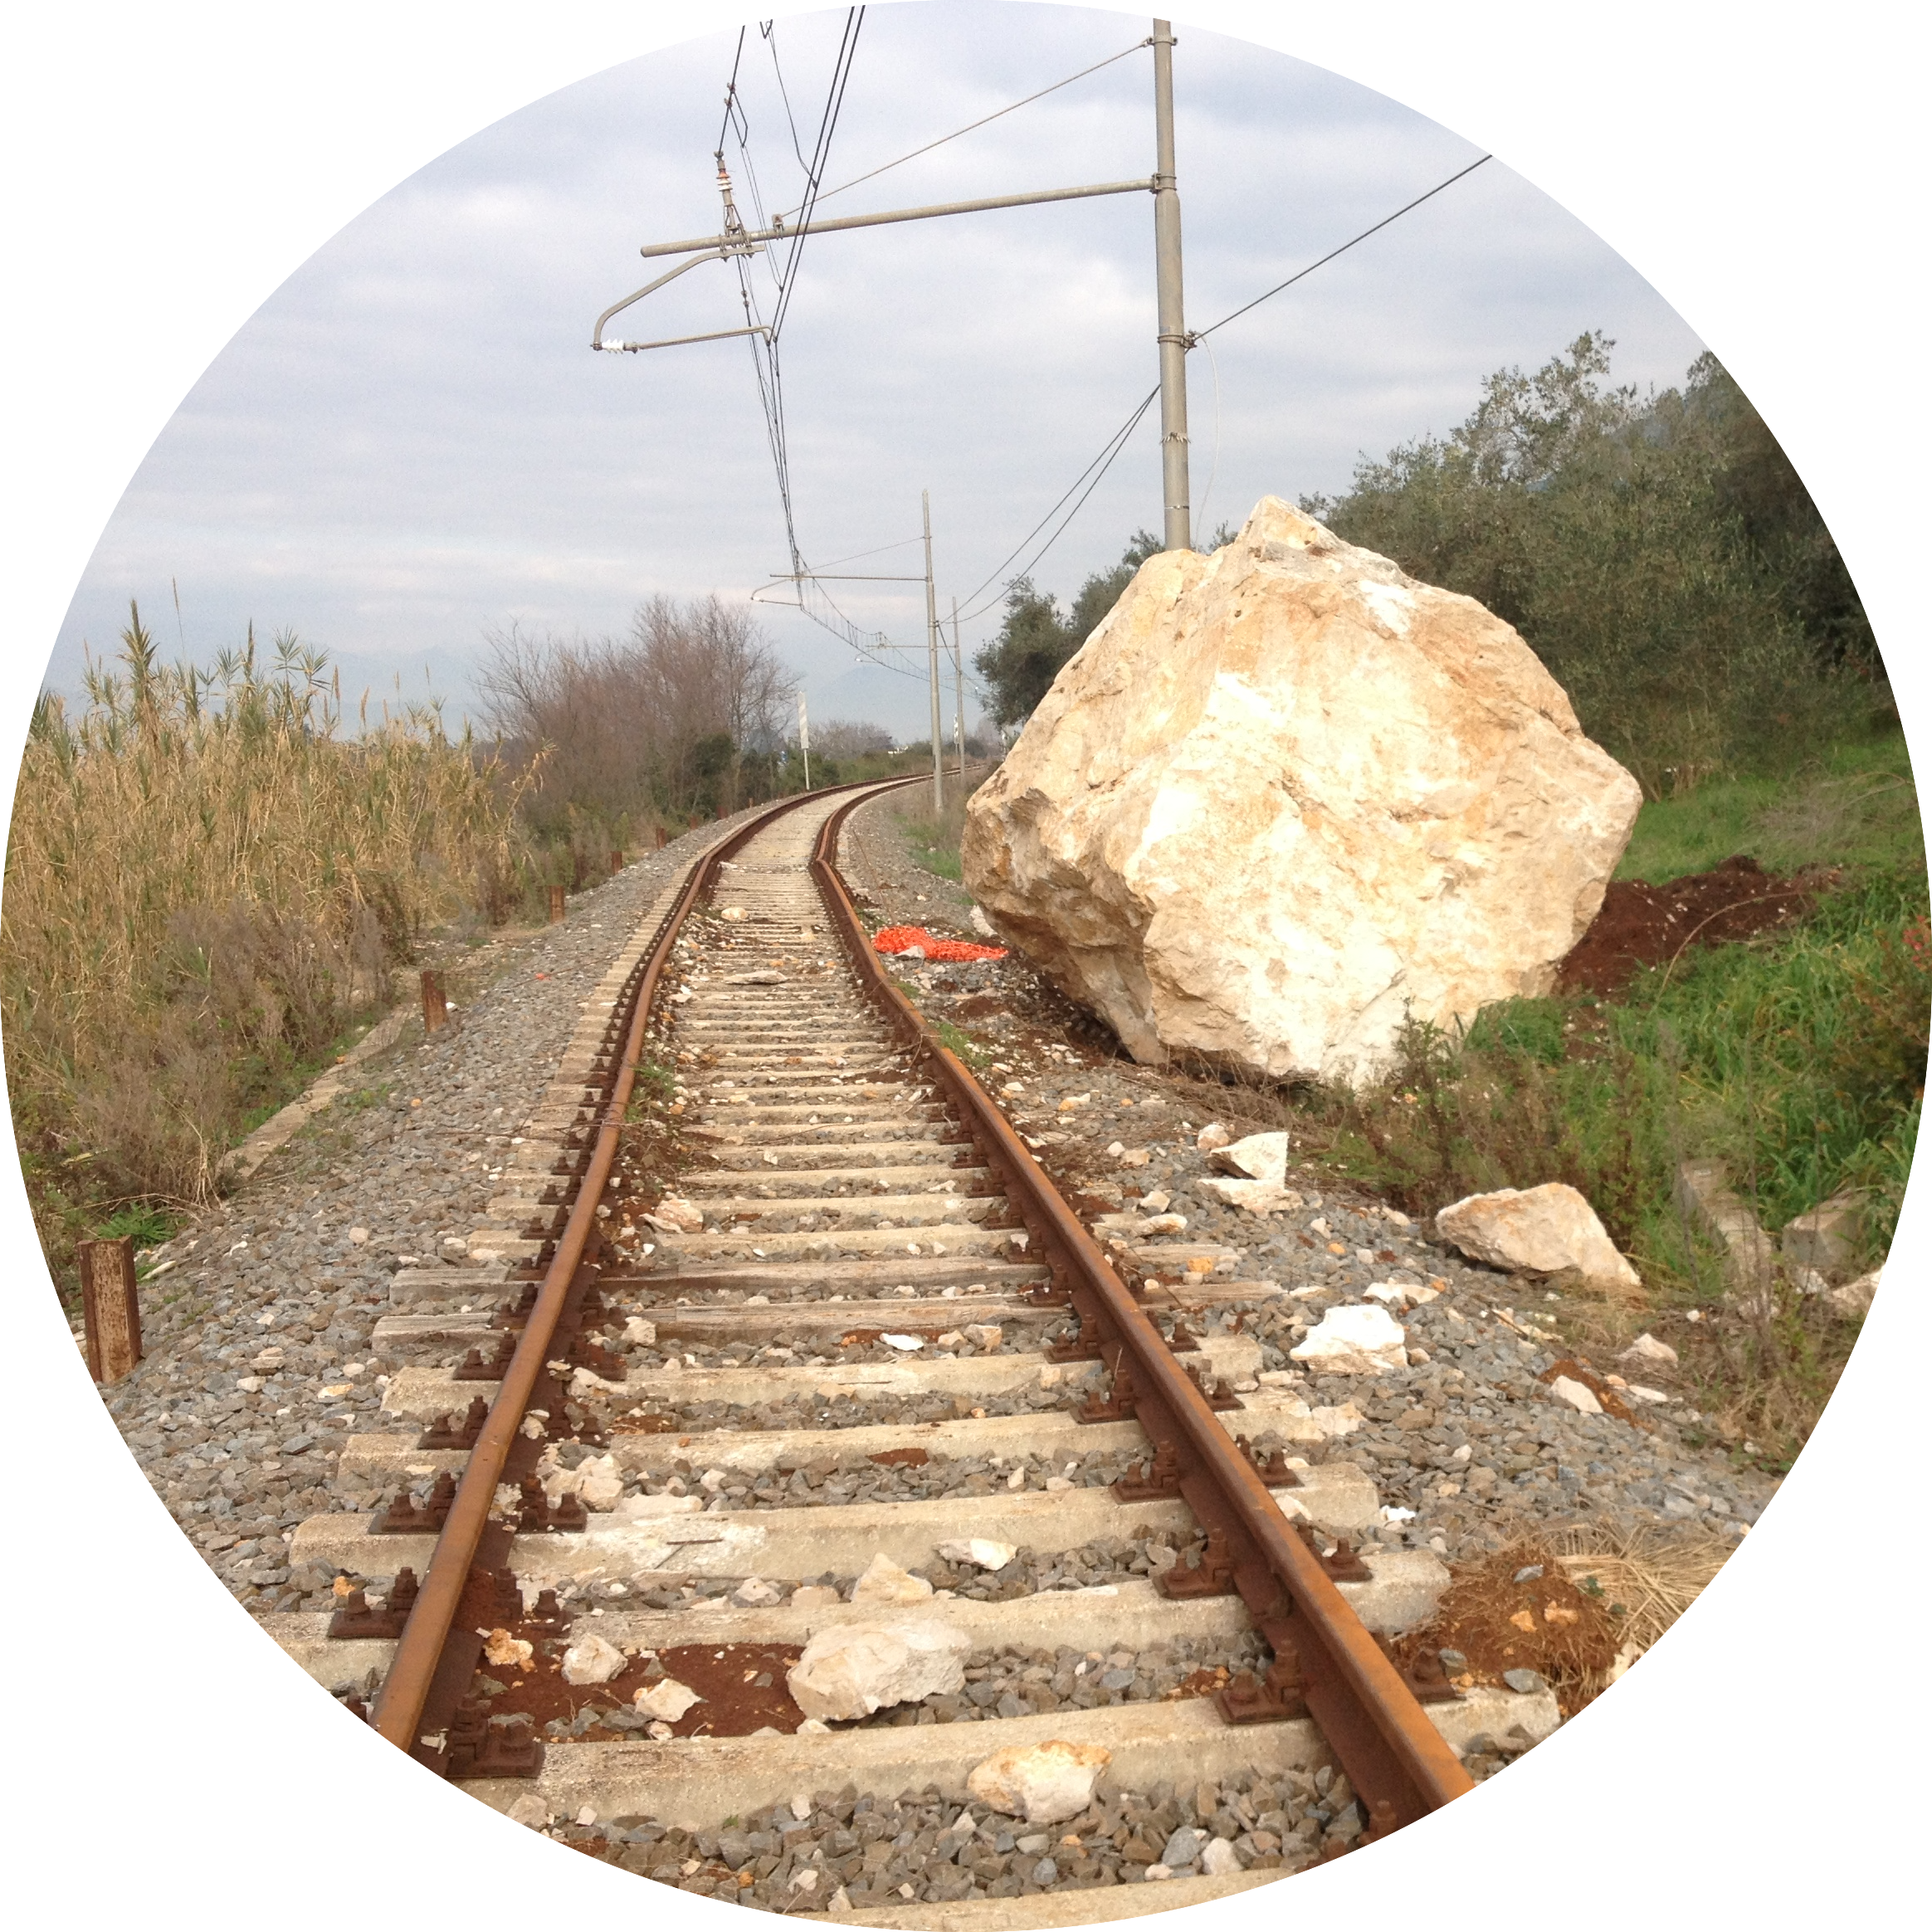
\includegraphics[width=10cm]{images/frontespizio} \\ \medskip % Picture

\vfill
\
Basi di Dati 2 \\ \medskip % Thesis subtitle
%\myDegree \\
Dipartimento di Ingegneria e Scienze dell'Informazione e Matematica \\
%\myFaculty \\
Università degli Studi Dell'Aquila \\ \bigskip

Giugno 2017 -- Versione 1.0 % Time and version

\vfill

\end{center}
\end{addmargin}

\end{titlepage} % Main title page

%\include{FrontBackMatter/Titleback} % Back of the title page

%\cleardoublepage\include{FrontBackMatter/Dedication} % Dedication page

%\cleardoublepage\include{FrontBackMatter/Foreword} % Uncomment and create a Foreword.tex to include a foreword

%\cleardoublepage\include{FrontBackMatter/Abstract} % Abstract page

%\cleardoublepage\include{FrontBackMatter/Publications} % Publications from the thesis page

%\cleardoublepage\include{FrontBackMatter/Acknowledgments} % Acknowledgements page

\pagestyle{scrheadings} % Show chapter titles as headings

\cleardoublepage\include{FrontBackMatter/Contents} % Contents, list of figures/tables/listings and acronyms

%\cleardoublepage

\pagenumbering{arabic} % Arabic page numbering for thesis content (1, 2, 3, etc)
%\setcounter{page}{90} % Uncomment to manually start the page counter at an arbitrary value (for example if you wish to count the pre-content pages in the page count)

\cleardoublepage % Avoids problems with pdfbookmark

%----------------------------------------------------------------------------------------
%	THESIS CONTENT - CHAPTERS
%----------------------------------------------------------------------------------------

% Chapter 1

\chapter{Introduzione} % Chapter title

\label{ch:introduction} % For referencing the chapter elsewhere, use \autoref{ch:introduction} 

Con il termine \textit{frana} si indicano tutti i fenomeni di movimento di terreno, come ad esempio caduta di rocce e  scivolamento di detriti superficiali, lungo un pendio.
La forza di gravità, a cui è soggetta la massa di terreno, è sicuramente la causa scatenante più importante ma non è l'unica. Una frana avviene nel momento in cui un pendio passa da una condizione di stabilità ad una di instabilità.
Tale passaggio di stato è causato da diversi fattori i quali possono contribuire contemporaneamente o singolarmente.
Tra le cause naturali sono evidenziati le seguenti:

\begin{enumerate}
	\item pressione di acqua sotterranea (acqua piana) che agisce per destabilizzare la pendenza;
	\item assenza di vegetazione (dovuta ad esempio ad un incendio);
	\item erosione della punta di un pendio;
	\item indebolimento di un pendio a causa di piogge pesanti o scioglimento di ghiacci/neve;
	\item terremoti che aggiungono carichi a pendenze già poco stabili.
\end{enumerate}
Il fenomeno delle frane è aggravato inoltre da fattori riconducibili alle attività umane come:
\begin{enumerate}
	\item deforestazioni e costruzioni che destabilizzano i pendii;
	\item sterri che alterano la forma dei pendii e che quindi posso aggiungere nuovi carichi.
\end{enumerate}
Una frana generalmente è caratterizzata dal tipo di materiale movimentato (ad esempio materiale roccioso o semplicemente detriti superficiali) e dal tipo di movimento che il materiale segue. Queste due caratteristiche principali vengono poi integrate considerando anche altri aspetti come la velocità e l'entità del movimento.
In base al comportamento della frana possiamo quindi avere la seguente classificazione: 
\begin{enumerate}
	\item \textbf{Frane di crollo:} massa che si stacca da un versante molto acclive e che, successivamente, si muove per caduta libera, rimbalzo, rotolamento. Il distacco può avvenire per rottura di taglio o di trazione della roccia (Figura \ref{crollo}).
	\item \textbf{Frane da ribaltamento:} rotazione in avanti, verso l'esterno del versante, di una massa di terra o roccia, intorno ad un punto situato al di sotto del baricentro della massa spostata (Figura \ref{ribaltamento}).
	\item \textbf{Frana da scivolamento planare:} movimento verso la base del versante di una massa di terra o roccia che avviene per deformazioni di taglio lungo una o più superfici o entro uno spessore limitato di materiale (Figura \ref{scivolamento}).
	\item \textbf{Frana da colata o colamento:} movimento distribuito in maniera continua all'interno della massa spostata. Le superfici di taglio, se presenti, sono multiple e spesso temporanee. La distribuzione delle velocità nella massa
	spostata è analoga a quella all'interno di un fluido viscoso  (Figura \ref{colata}).
\end{enumerate}

\begin{figure}[h]
	\hspace{0.1\linewidth}
	\begin{minipage}[t]{0.35\linewidth}
		\centering
		\includegraphics[width=\textwidth]{images/crollo}
		\caption{Frana di crollo. I massi che si staccano dalla cima rotolano lungo il pendio e arrivano a valle. }
		\label{crollo}
	\end{minipage}
	\hspace{0.1\linewidth}
	\begin{minipage}[t]{0.35\linewidth}
		\centering
		\includegraphics[width=\textwidth]{images/Ribaltamento}
		\caption{Frana di ribaltamento. Un'intera parete rocciosa si distacca dal pendio.}
		\label{ribaltamento}
	\end{minipage}
\end{figure}

\begin{figure}[h]
	\hspace{0.1\linewidth}
	\begin{minipage}[t]{0.35\linewidth}
		\centering
		\includegraphics[width=\textwidth]{images/Scivolamento_planare}
		\caption{Frana da scivolamento planare. Un'area di terreno intera scivola verso la valle.}
		\label{scivolamento}
	\end{minipage}
	\hspace{0.1\linewidth}
	\begin{minipage}[t]{0.35\linewidth}
		\centering
		\includegraphics[width=\textwidth]{images/colata}
		\caption{Frana da colata. I detriti scivolano verso la valle formando un corridoio. }
		\label{colata}
	\end{minipage}
\end{figure}

Rispetto a questa classificazione è possibile trarre alcune conclusioni riguardo l'andamento spaziale di una frana.  Innanzitutto è complicato stimare lo spazio percorso dalla frana. Prendendo, ad esempio, in considerazione una frana di crollo la distanza percorsa dal masso dipende da un numero elevato di variabili fisiche tra loro correlate (accelerazione, velocità, urti, massa ecc ecc). E' ragionevole però, con la dovuta prudenza che il caso richiede, stabilire un raggio di azione della frana, oltre il quale il fenomeno non può proseguire. Del resto un masso, dopo aver rotolato lungo un pendio, possiede un quantitativo limitato di energia meccanica la quale verrà a poco a poco dissipata lungo il tratto non in pendenza fino ad esaurirsi completamente (Figura \ref{distanzaFrana}). 

\begin{figure}[h]
	\centering
	\includegraphics[width=0.7\textwidth]{images/distanza_frana}
	\caption{Rappresentazione di una frana di crollo. Il masso si stacca sulla cima del pendio e scende già aumentando la sua energia meccanica. Finito il pendio l'energia meccanica accumulata diminuisce fino ad esaurirsi. Il punto esatto dove si ferma il masso non è dato saperlo, ma si può stimare una distanza d oltre la quale ragionevolmente il masso non potrà spingersi.}
	\label{distanzaFrana}
\end{figure}

Un'altra osservazione la si può dedurre analizzando le fotografie scattate nei luoghi dove si sono verificate delle frane. In molti casi, soprattutto nei casi di frana da colamento, il terreno movimentato segue una traiettoria ben precisa (Figura \ref{traiettoriaFrana}). Quest'ultima dipende dalla morfologia del pendio, ovvero da come sono distribuite le masse di terreno lungo la discesa. Anche in questo caso è possibile stabilire un raggio d'azione inteso come la larghezza del "corridoio" dentro il quale la frana scivola (Figura \ref{traiettoriaFrana2}). Infine bisogna sempre tenere a mente che la forza di gravità è il fattore scatenante per eccellenza della frana, motivo per cui la pendenza del terreno giocherà sempre un ruolo fondamentale.

\begin{figure}[h]
	\centering
	\includegraphics[width=0.7\textwidth]{images/traiettoria_frana}
	\caption{Frana di Colonia Las Colinas, El Salvador, 2001. E' possibile osservare come, in questo caso, la frana ha seguito una traiettoria ben delimitata tipica delle frane di colata. In questo caso specifico la distanza percorsa dalla frana è stata pari a circa 700 metri \textcolor{red} {(URL!!!!!!!!!!!!)}.}
	\label{traiettoriaFrana}
\end{figure}


\begin{figure}[h]
	\centering
	\includegraphics[width=0.7\textwidth]{images/traiettoria_frana2}
	\caption{Rappresentazione di una frana di colamento. E' possibile definire un raggio di azione r inteso come l'ampiezza del "corridoio" della frana.}
	\label{traiettoriaFrana2}
\end{figure}

La caratterizzazione di una frana è fondamentale e propedeutica ad enucleare una efficace strategia di prevenzione. Poter disporre di una strategia di questo tipo è particolarmente rilevante nel caso in cui l'ente che la mette in pratica ha un numero di \textit{assets strategici} molto elevato. Prendiamo in considerazione, solo per citare un esempio, Ferrovie dello Stato Italiane Spa. L'azienda possiede, tra i suoi assets, una rete ferroviaria di 16734 Km e più di 3,000 stazioni dislocate su un territorio (L'Italia) la cui superficie è di 301,340 $Km^2$. E' impensabile che i vertici delle Ferrovie dello Stato approvino un piano aziendale di prevenzione che preveda il controllo di ciascuna stazione e ciascun Km della rete ferroviaria! Sarebbe impossibile sia in termini di tempo necessario che di sforzo economico che l'Ente dovrebbe sostenere. 

La soluzione ideale sarebbe quella di avere un metodo che prenda in input un insieme di assets strategici e restituisca come output un lista ordinata in base alla loro esposizione al rischio frana. In questo modo sarebbe possibile occuparsi degli assets che sono veramente a rischio e quindi, oltre a risparmiare denaro, essere più rapidi negli interventi.

Il metodo da noi proposto verrà illustrato nelle prossime sezioni del documento. In particolare nella sezione 2 vengono fornite le definizioni dei concetti base, fondamentale per la comprensione del metodo, attraverso una formulazione matematica. Nella sezione 3 verrà spiegato in che modo le considerazioni fatte sulla pendenza del terreno e le traiettorie delle frane sono state affrontate e tradotte in equazioni matematiche. Infine nella sezione 4 verrà esposto come tali equazioni vengono utilizzate nello pseudo-codice dell'algoritmo.
 % Indroduzione
% Chapter 2

\chapter{Notazioni e definizioni} % Chapter title

\label{ch:notazioni} % For referencing the chapter elsewhere, use \autoref{ch:examples} 

\begin{enumerate}
	
	\item \label{def:geoarea} \textit{GeoArea} : Definisce un territorio di interesse per il calcolo dell'esposizione a rischio frana. La \textit{GeoArea} può rappresentare un comune, una provincia (Figura \ref{RomaBoundary}), una regione (Figura \ref{LazioBoundary}), una nazione (Figura \ref{ItaliaBoundary}) fino ad arrivare ad un intero continente. GeoArea è descritta dalla tupla <\textit{ID}, \textit{description}, \textit{boundary}>.
	
	\begin{figure}[h]
		\hspace{0.02\linewidth}
		\begin{minipage}[t]{0.3\linewidth}
			\centering
			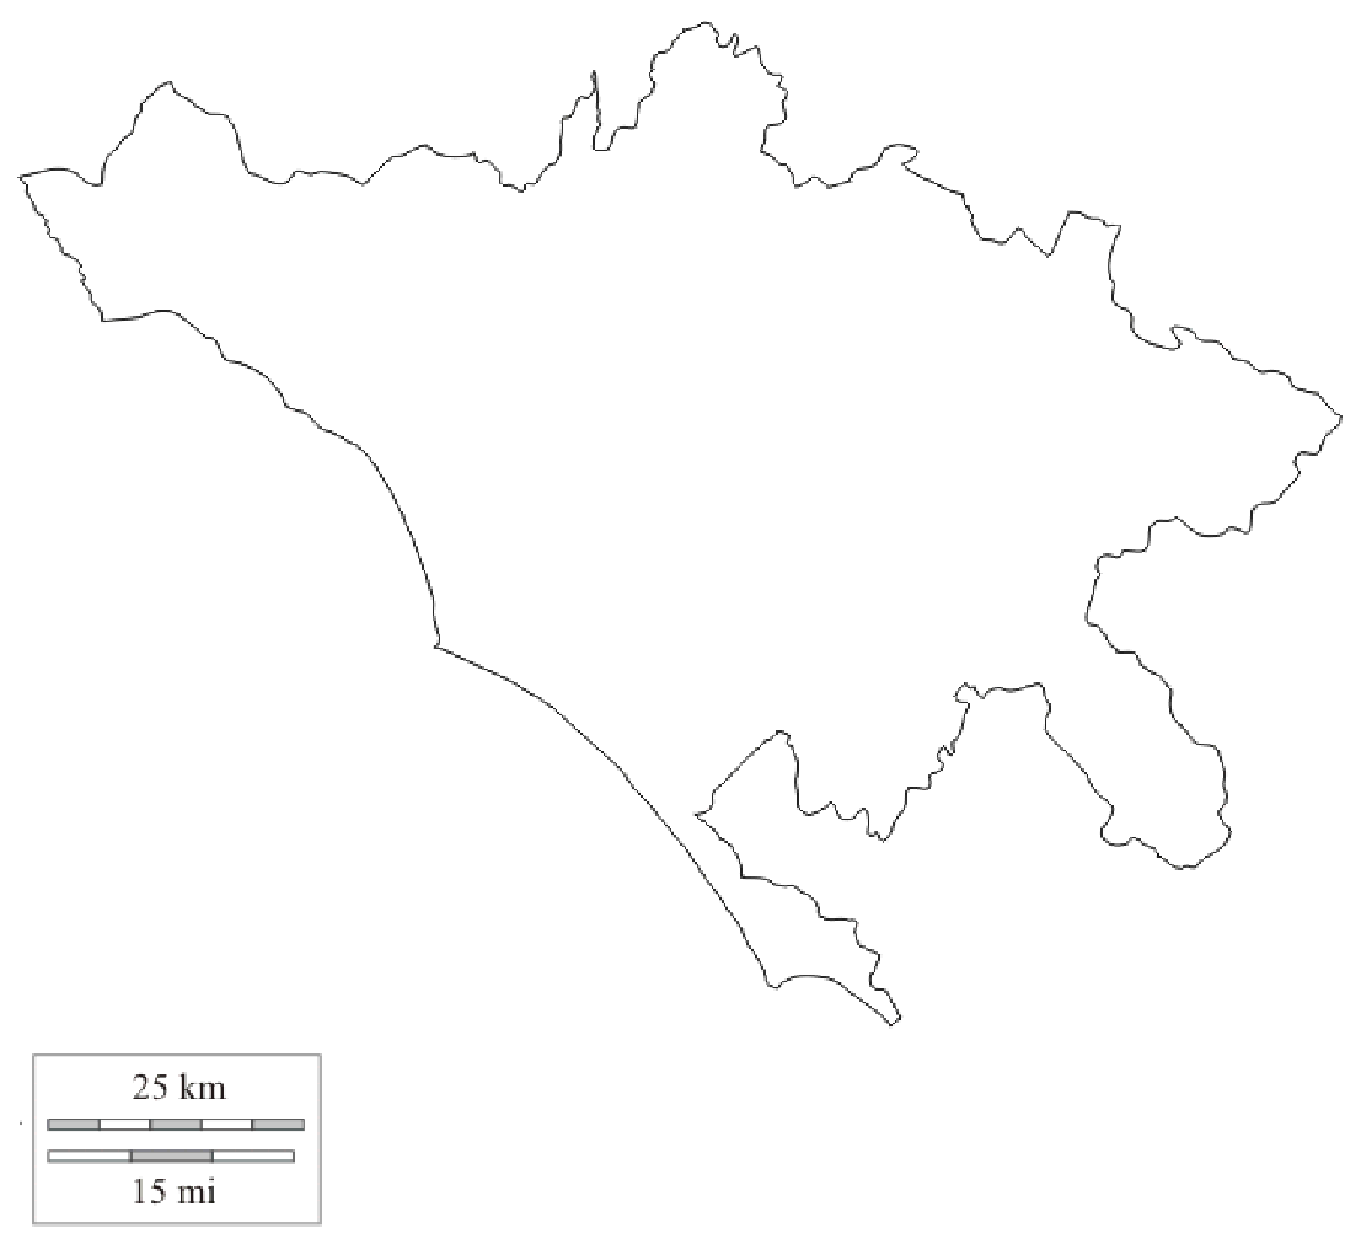
\includegraphics[width=1\textwidth]{images/roma}
			\caption{Confini della provincia di Roma.}
			\label{RomaBoundary}
		\end{minipage}
		\hspace{0.03\linewidth}
		\begin{minipage}[t]{0.3\linewidth}
			\centering
			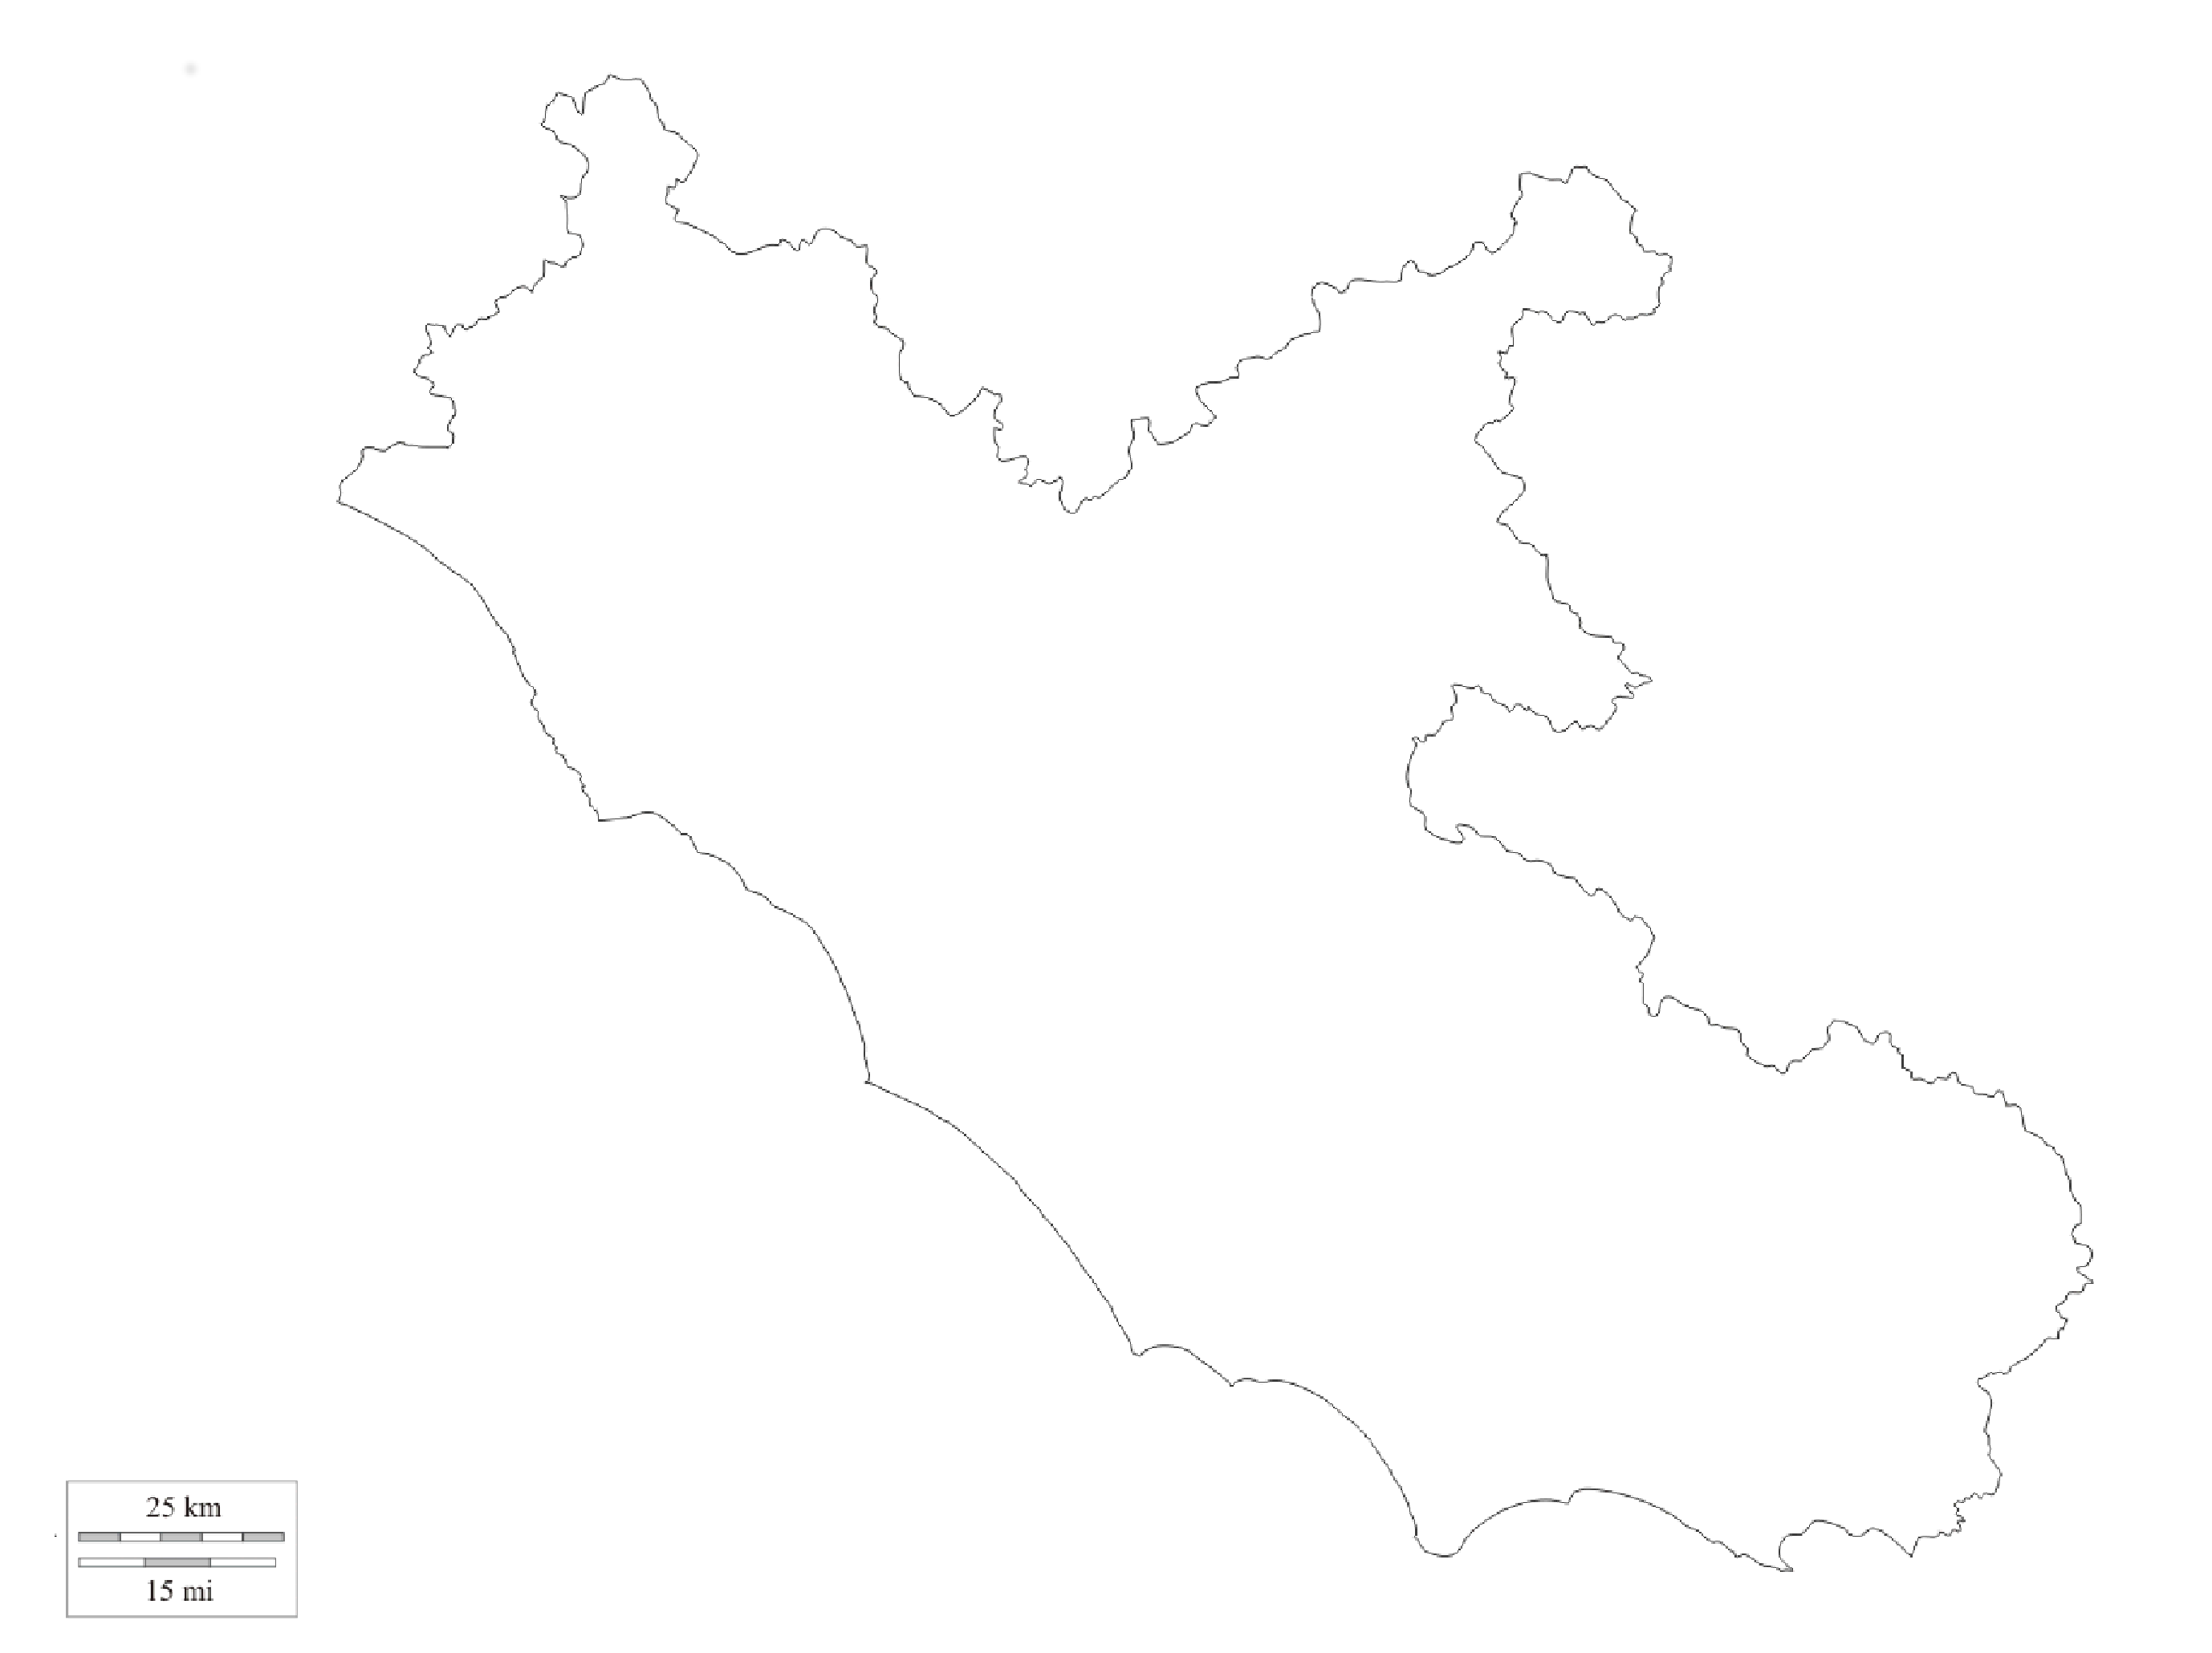
\includegraphics[width=1\textwidth]{images/lazio}
			\caption{Confini della regione Lazio.}
			\label{LazioBoundary}
		\end{minipage}
		\hspace{0.02\linewidth}
		\begin{minipage}[t]{0.3\linewidth}
			\centering
			
\includegraphics[width=1\textwidth]{images/italia}
			\caption{Confini del territorio italiano.}
			\label{ItaliaBoundary}
		\end{minipage}
	\end{figure}
	
	
	\item \label{def:zones} \textbf{$ \mathcal{Z} $ (Zones)} $ = \{ z_k(k=1,2,..) | z_k $ \`e una \textit{Zone} di  GeoArea \}. Una \textit{Zone} definisce una porzione di terreno all'interno della GeoArea ed è descritta dalla tupla <\textit{ID}, \textit{boundary}, \textit{$Sz_k$}>. Il campo \textit{ID} identifica univocamente la k-esima \textit{Zone}, \textit{boundary} la geometria del confine e \textit{$Sz_k$} è un valore decimale che rappresenta la probabilità di frana di $z_k$ (Figura \ref{Zk}).
	Si noti che $zk$ è una notazione sovraccaricata in quanto rappresenta sia l’\textit{ID} di una \textit{Zone} che la sua geometria.
	
	\begin{figure}[h]
		\centering
		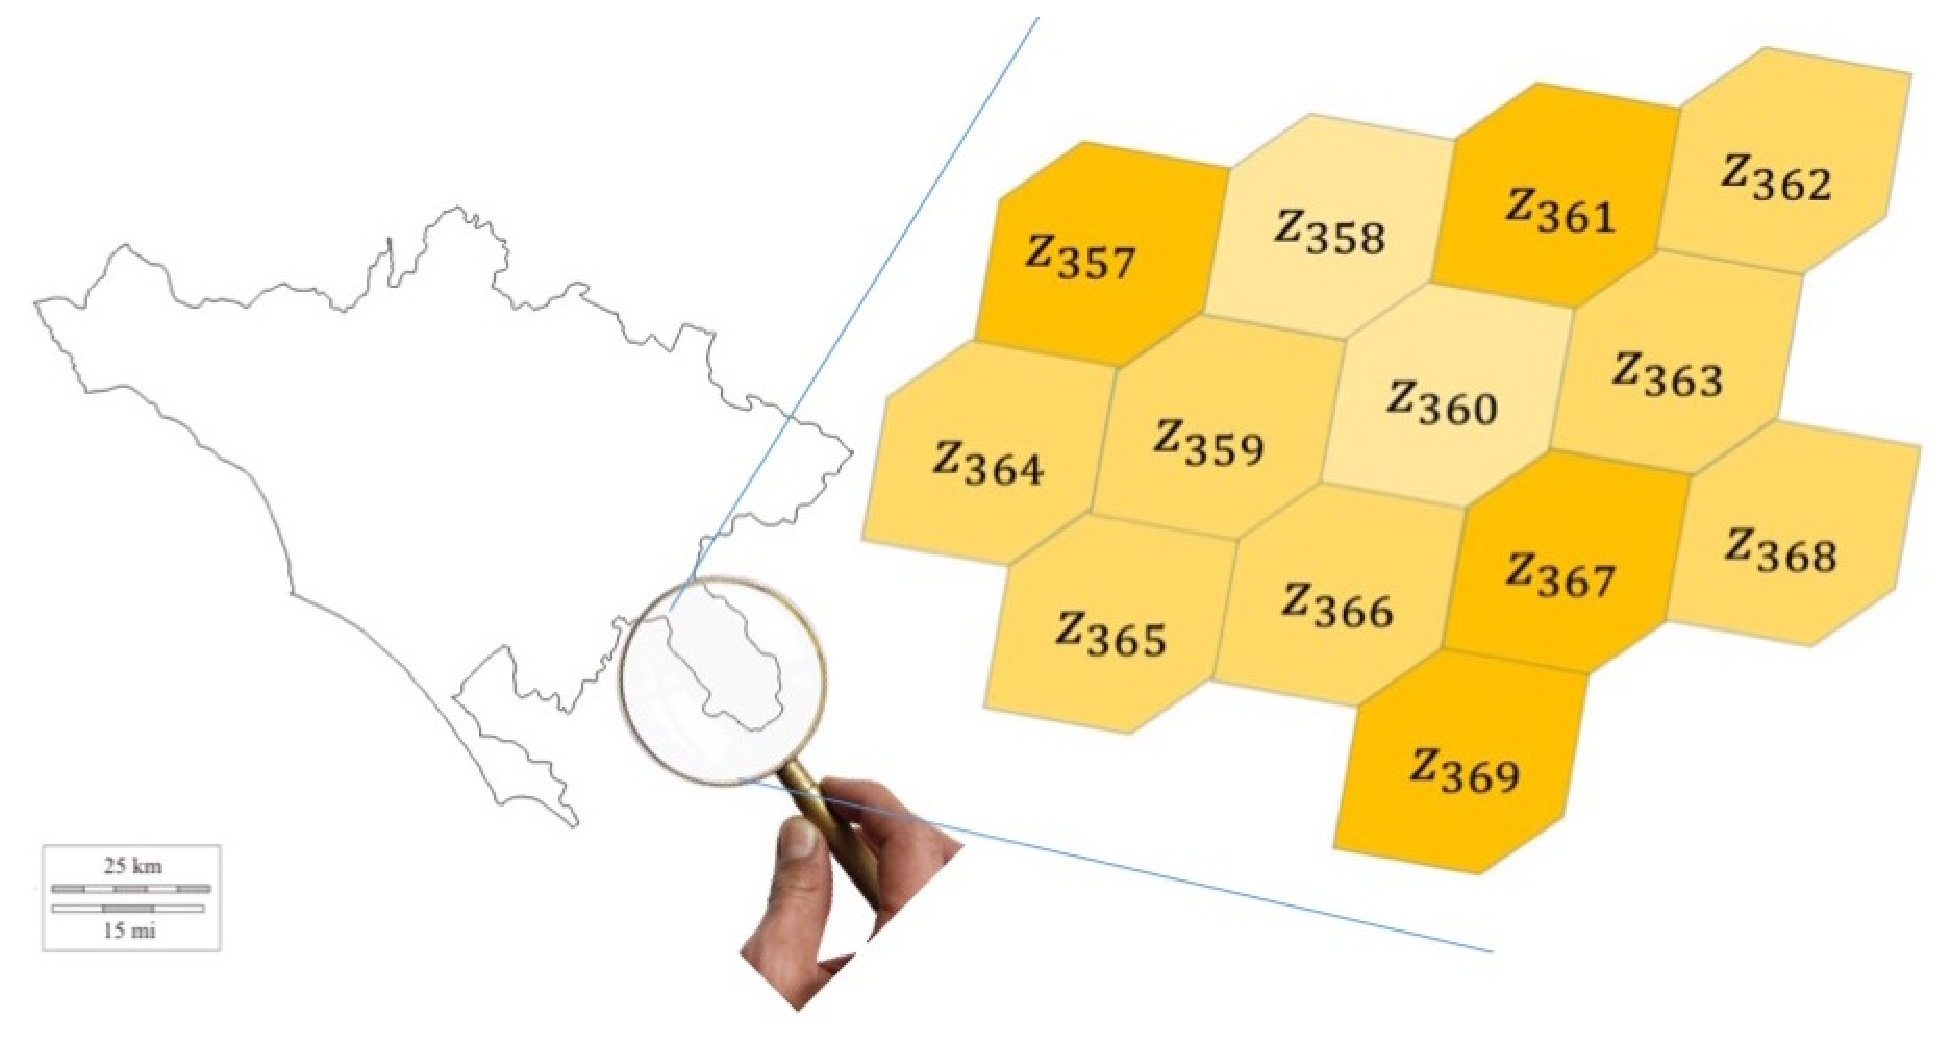
\includegraphics[width=0.7\textwidth]{images/zk}
		\caption{Rappresentazione delle Zones di una \textit{GeoArea}. La geometria del confine delle porzioni di terreno è puramente indicativa. Le diverse tonalità di arancione rappresentano i valori di $Sz_k$  delle \textit{Zones}.}
		\label{Zk}
	\end{figure}
	
	\item \textbf{$ \mathcal{B} $ (Buildings)} $ = \{b_i(i=1,2,..) | b_i $ è un \textit{building} ubicato all'interno dei confini della  GeoArea \}. Per building si intende un generico edificio (come ad esempio una scuola, un grattacielo, un hotel e strutture simili) descritto dalla tupla < \textit{ID}, \textit{description}, \textit{position}>. Il campo \textit{ID} identifica univocamente l'edificio; \textit{description} una sua descrizione testuale e infine \textit{position} rappresenta la posizione geografica di $ b_i $ espressa da una coppia di coordinate geografiche (Figura \ref{station}). Definiamo con $\mathbf{card}(\mathcal{B})$ la cardinalità dell'insieme $ \mathcal{B} $, ovvero il numero di edifici presenti in \textit{GeoArea}. Dettagli come la planimetria della struttura potrebbero fornire ulteriori dati sensibili ma sono molto difficili da reperire e quindi non verranno presi in considerazione.
	In seguito verrà usato sempre il pedice $i$ per riferirsi al building $i-esimo$.
	Nelle notazioni introdotte di seguito l'occorrenza del pedice $i$ viene usata $sempre$ per richiamare che ci si riferisce all'edificio $i-esimo$, ovvero all'elemento $b_i$ di $ \mathcal{B} $.
	
	\item \textbf{$HazardArea_i$} rappresenta l'area a possibile rischio smottamento circostante l'edificio $b_i$, definita come la circonferenza centrata su $b_i$ di raggio $r$ (Figura \ref{buffer}).
	
	\begin{figure}[h]
		\hspace{0.1\linewidth}
		\begin{minipage}[t]{0.35\linewidth}
			\centering
			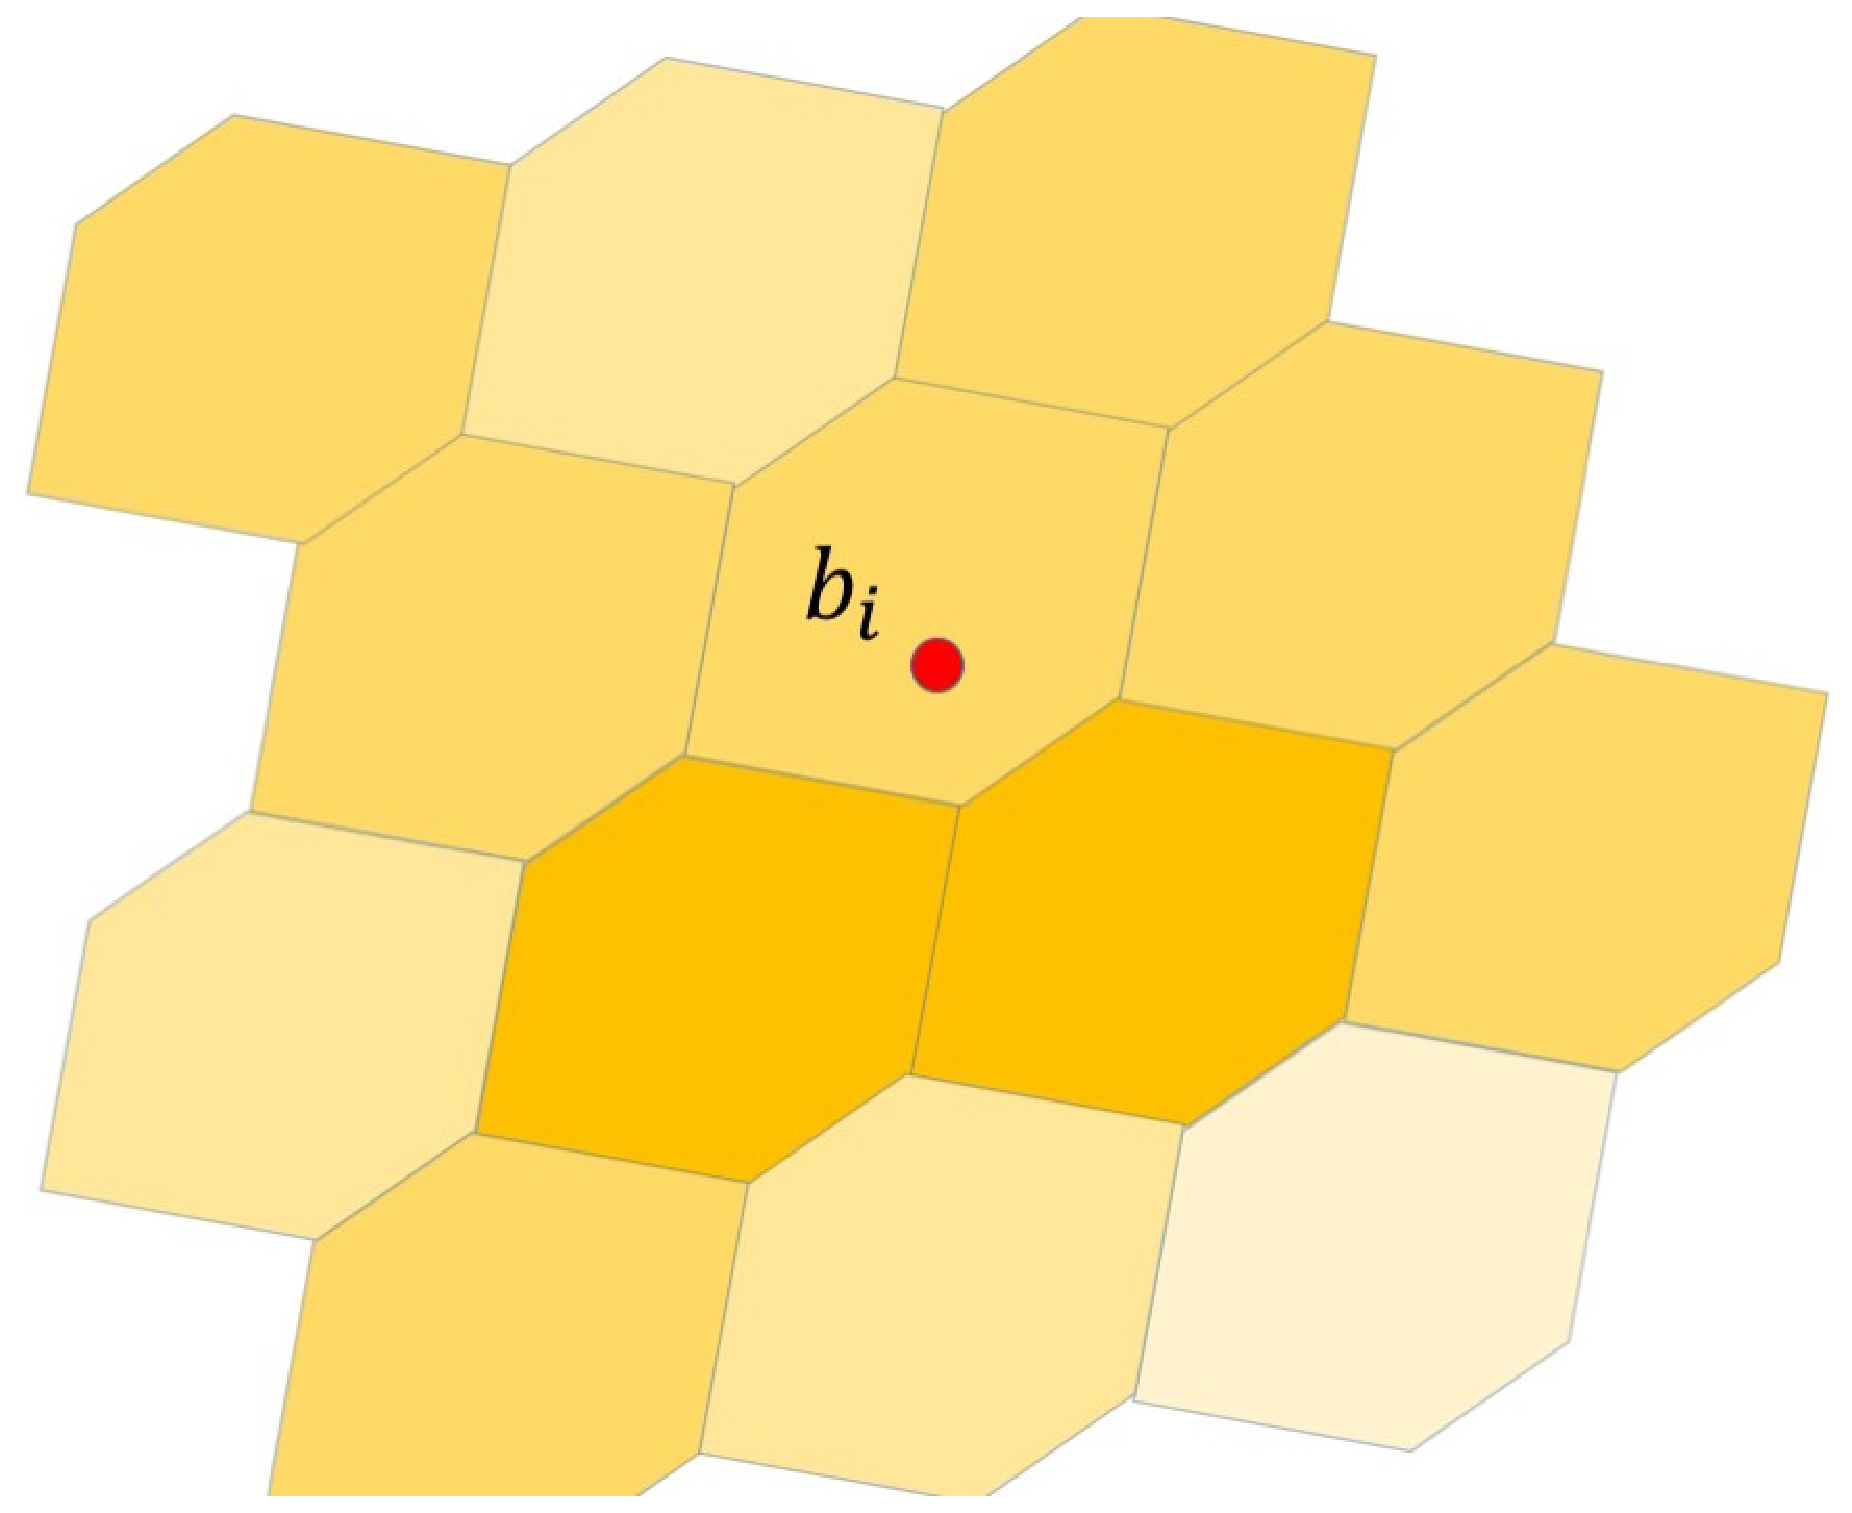
\includegraphics[width=1\textwidth]{images/station}
			\caption{Il pallino rosso rappresenta il generico edificio $b_i$.}
			\label{station}
		\end{minipage}
		\hspace{0.13\linewidth}
		\begin{minipage}[t]{0.35\linewidth}
			\centering
			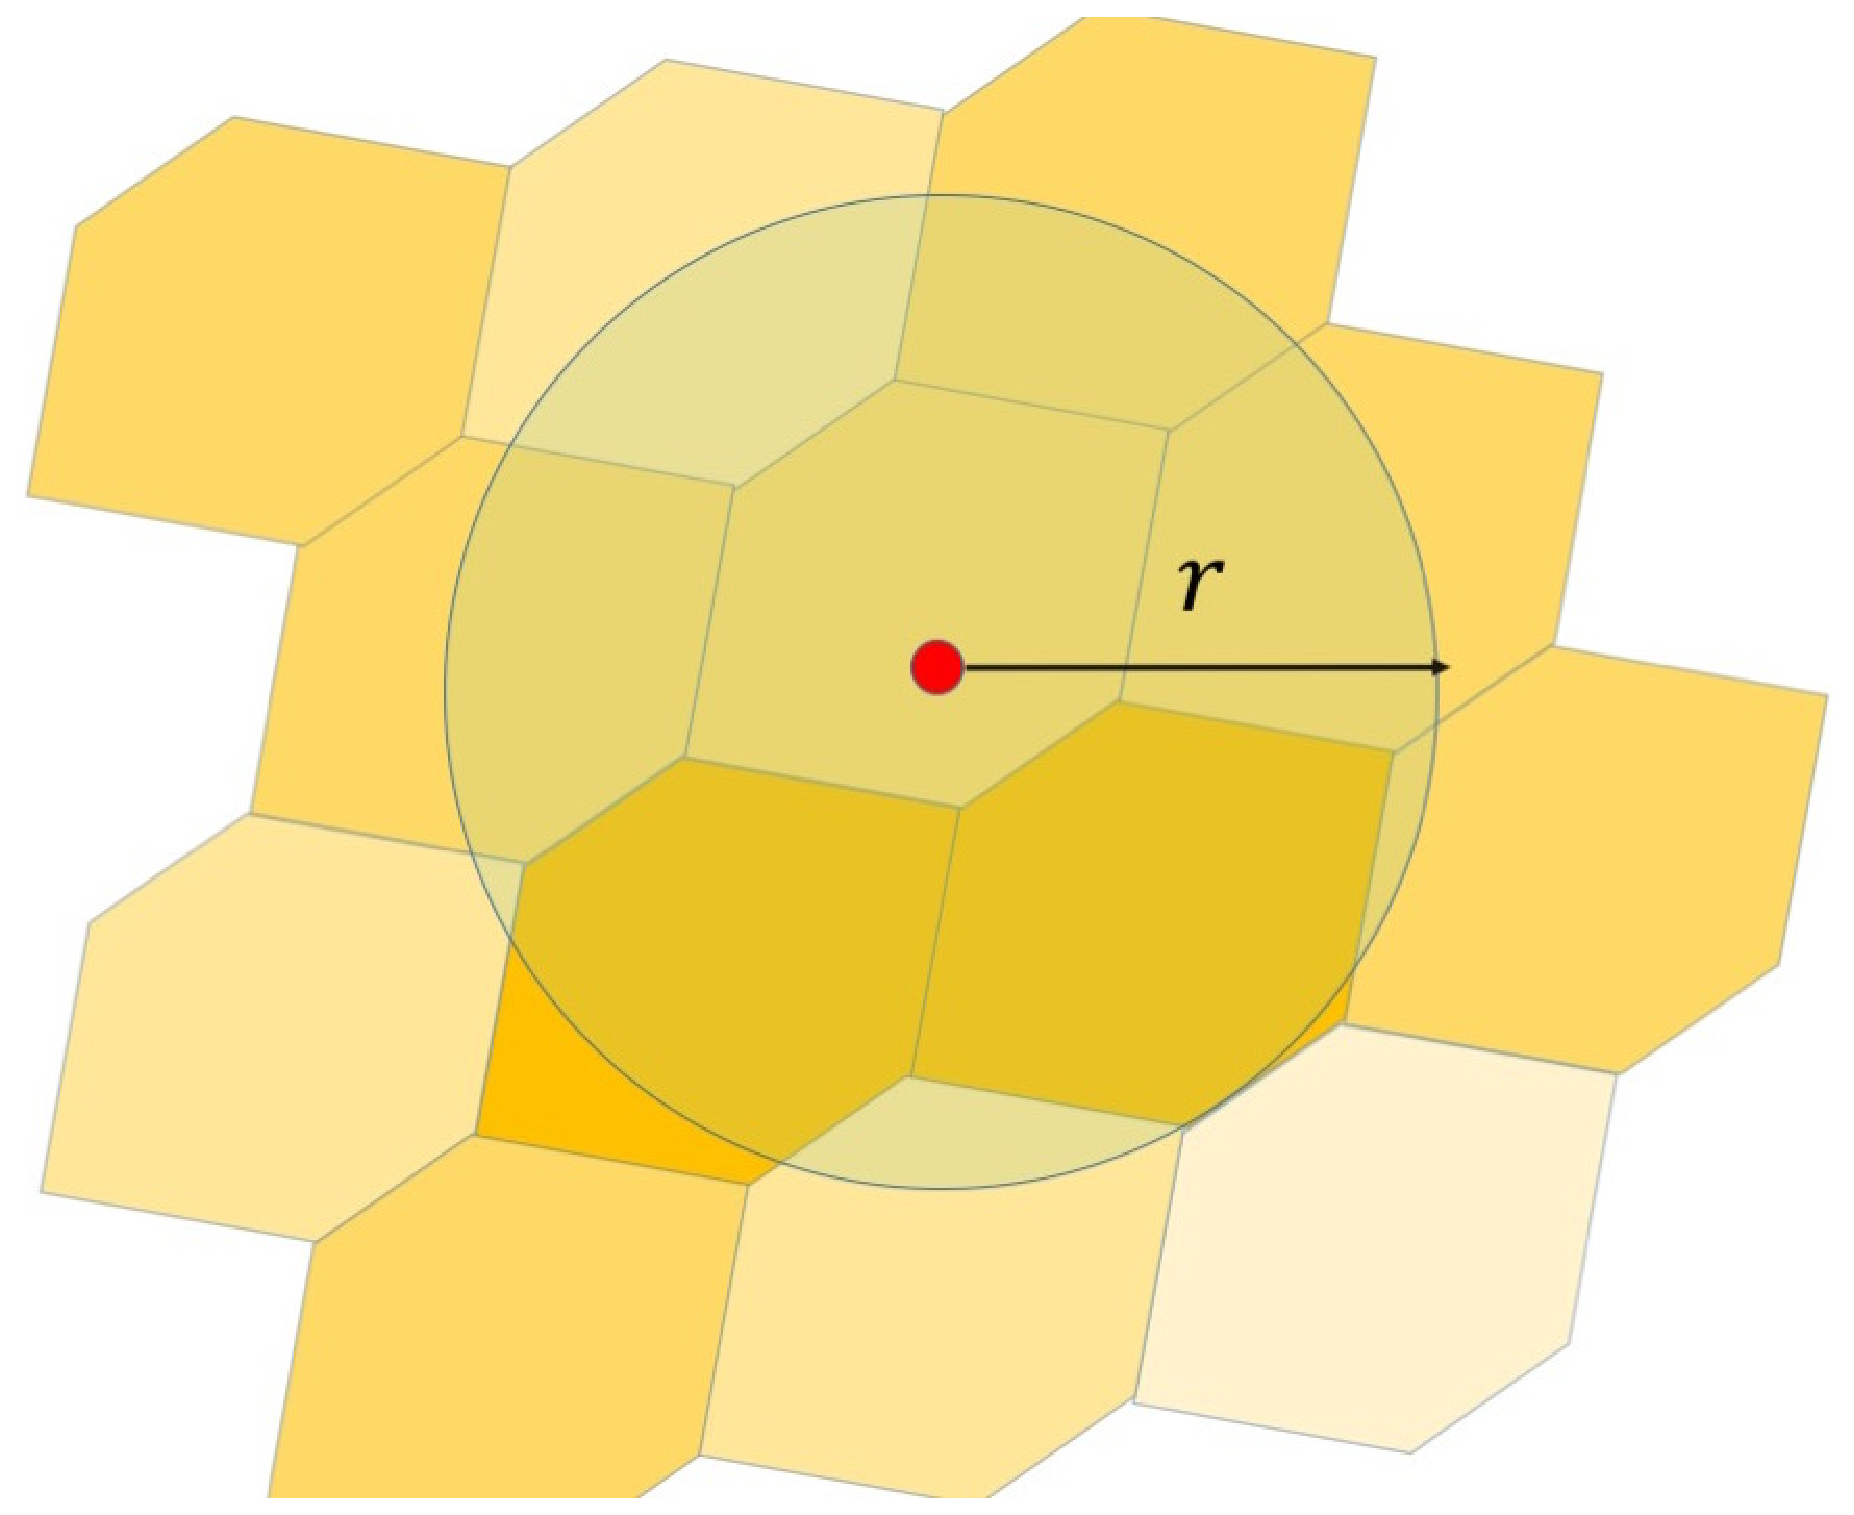
\includegraphics[width=1\textwidth]{images/buffer}
			\caption{In verde chiaro \`e rappresentato il buffer di raggio $r$ centrato  sull'edificio $b_i$. }
			\label{buffer}
		\end{minipage}
	\end{figure}
	
	\item \textbf{$ \mathcal{NZ}_i $ (Nearest Zones)} $ = \{nz_{i,j}(i=1,..,\mathbf{card}( \mathcal{B} )), (j=1,..,\mathbf{card}(\mathcal{ NZ}_i)) | nz_{i,j} \in  \mathcal{Z}  \cap HazardArea_i $ è una \textit{Nearest Zone}, ovvero 	una \textit{Zone} che si trova all'interno della $HazardArea_i$ di $b_i$\}. Gli $nz_{i,j}$ possono rappresentare le \textit{Zones} nella loro interezza, oppure parte di esse derivante dall'intersezione con la $HazardArea_i$.  (Figura \ref{NearestLand}).
	In seguito verrà usato sempre il pedice $\mathbf{j}$ accostato al pedice $\mathbf{i}$ per riferirsi alla nearest zone j-esima del building i-esimo.
	Nelle notazioni introdotte di seguito l'occorrenza del pedice $\{i,j\}$ viene usata $sempre$ per richiamare che ci si riferisce alla nearest zone $j-esima$ dell'edificio $i-esimo$, ovvero all'elemento $nz_{i,j}$ di $ \mathcal{NZ}_i $.
	Si noti che $nz_{i,j}$ è una notazione sovraccaricata in quanto rappresenta sia l’\textit{ID} di una \textit{Nearest Zone} che la sua geometria.
	
	\item \textbf{$ cnz_{i,j} $ (Centroid of $nz_{i,j})$} corrisponde al centro di massa di $nz_{i,j}$ la cui posizione è descritta dalle sue coordinate geografiche (Figura \ref{cnz}). 
	
	\item \textbf{$ \mathcal{I} $} $ = \{i_p(p=1,2,..) | i_p $ \`e una \textit{isoipse} della GeoArea\}. Per isoipse si intende quella curva che unisce punti con uguale quota, descritta dalla tupla <\textit{ID}, \textit{elevation}, \textit{geometry}>. Il campo \textit{ID} identifica univocamente la curva di livello, \textit{elevation} la quota  e infine \textit{geometry} la geometria che descrive l'andamento dell'isoipse.
	
	\item \textbf{$ \mathcal{NI}_i $ (Nearest Isoipses)} $ = \{ ni_{i,o}(i=1,..,\mathbf{card}( \mathcal{B} )), (o=1,. . ,\mathbf{card}(\mathcal{ NI}_i)) | ni_{i,o} \in  \mathcal{I}  \cap HazardArea_i$ è la o-esima \textit{Nearest Isoipse} che si trova all'interno della $HazardArea_i$ di $b_i$ \}. Le $ni_{i,o}$ possono rappressentare le \textit{isoipse} nella loro interezza, oppure una parte di esse derivanti dall'intersezione con la $HazardArea_i$  (Figura \ref{NearestIso}). Si noti che $ni_{i,o}$ è una notazione sovraccaricata in quanto rappresenta sia l’\textit{ID} di una \textit{Nearest Isoipse} che la sua geometria.
	
	\begin{figure}[h]
		\hspace{0.05\linewidth}
		\begin{minipage}[t]{0.45\linewidth}
			\centering
			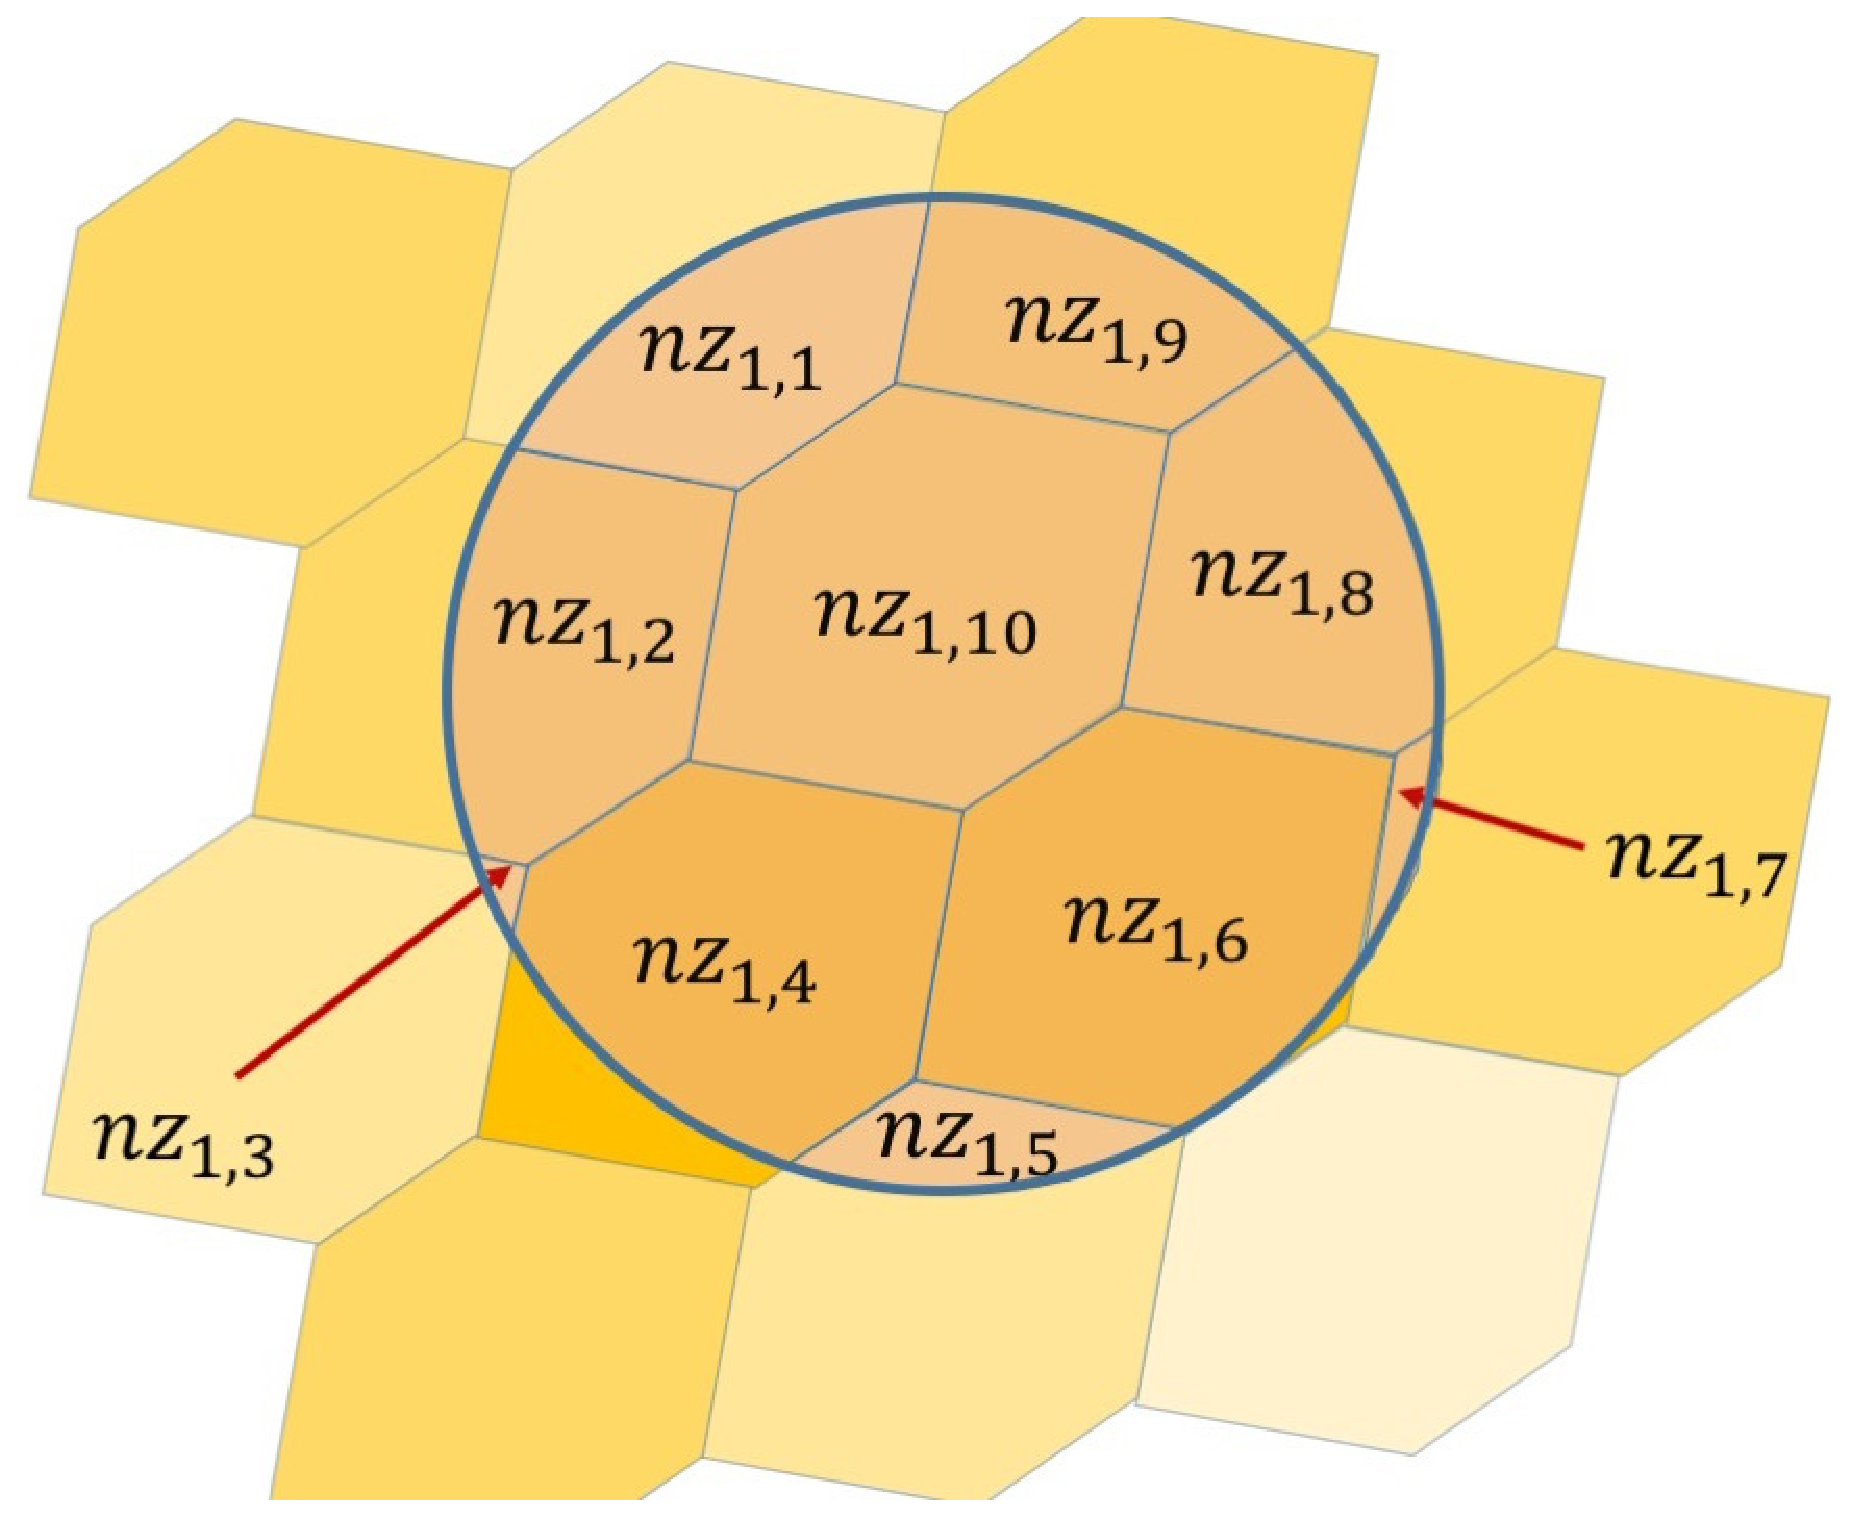
\includegraphics[width=1\textwidth]{images/NearestZone}
			\caption{In rosa sono rappresentate le $nz_{i,j}$ con $i=1$  che si trovano all'interno della $HazardArea_i$. E' possibile notare come $nz_{1,10}$ sia una \textit{Zone} intera mentre $nz_{1,3}$ è parziale.}
			\label{NearestLand}
		\end{minipage}
		\hspace{0.05\linewidth}
		\begin{minipage}[t]{0.45\linewidth}
			\centering
			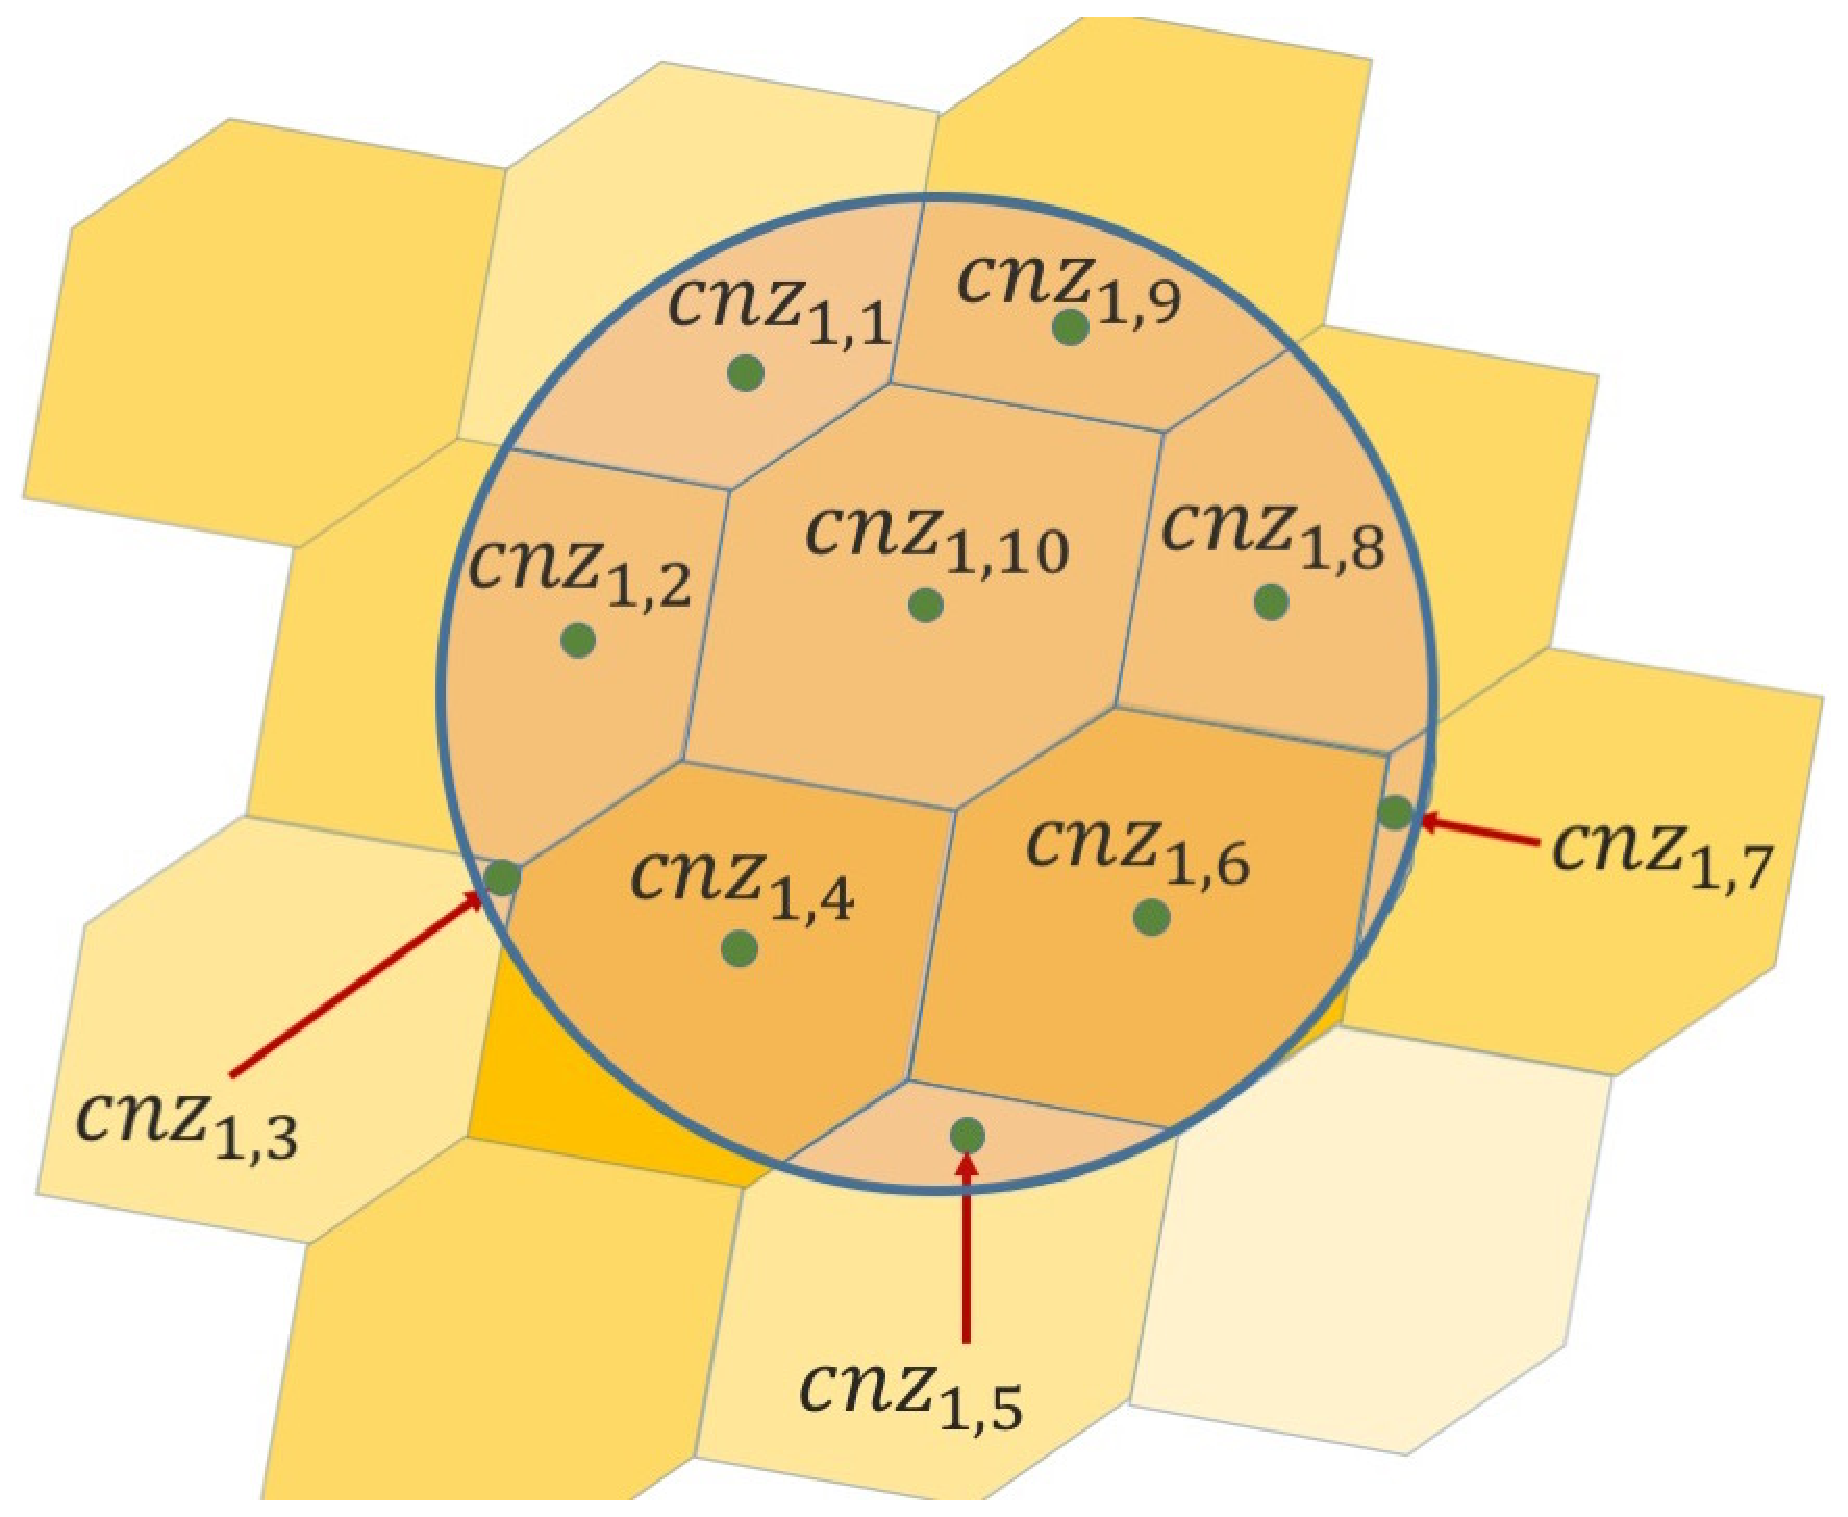
\includegraphics[width=1\textwidth]{images/cnz}
			\caption{Con i pallini verdi sono rappresentati i centri di massa $cnz_{i,j}$ degli $nz_{1,j}$.}
			\label{cnz}
		\end{minipage}
	\end{figure}
	
	\item \textbf{$\mathcal{ZF}_i$ (Zone Fragments)} $ = \{ zf_{i,j,t} (i=1,..,\mathbf{card}(\mathcal{B}),j=1,..,\mathbf{card}(\mathcal{NZ}_i),(t=1,..))| zf_{i,j,t}  $ è la t-esima \textit{Zone Fragment} interna alla nearest zone $nz_{i,j}$ restituita dall'operazione di splitting di detta nearest zone con le sole nearest isoipse in $\mathcal{NZ}_i $ che l'attraversa.
	I quattro poligoni in blu con i contorni gialli della Figura \ref{zf} rappresentano gli altrettanti \textit{Zone Fragments} nei quali la Nearest Zone $nz_{1,j}$ viene frammentata dall'operazione di split con le tre isoipse che la attraversano. $\mathcal{ZF}_i$ è l'insieme delle zone fragments prodotte dallo split tra gli $nz_{i,j} \in \mathcal{NZ}_i $ e le $ni_{i,o} \in \mathcal{NI}_i$ (Figura \ref{zf}). 
	
	
	\begin{figure}[h]
		\hspace{0.05\linewidth}
		\begin{minipage}[t]{0.45\linewidth}
			\centering
			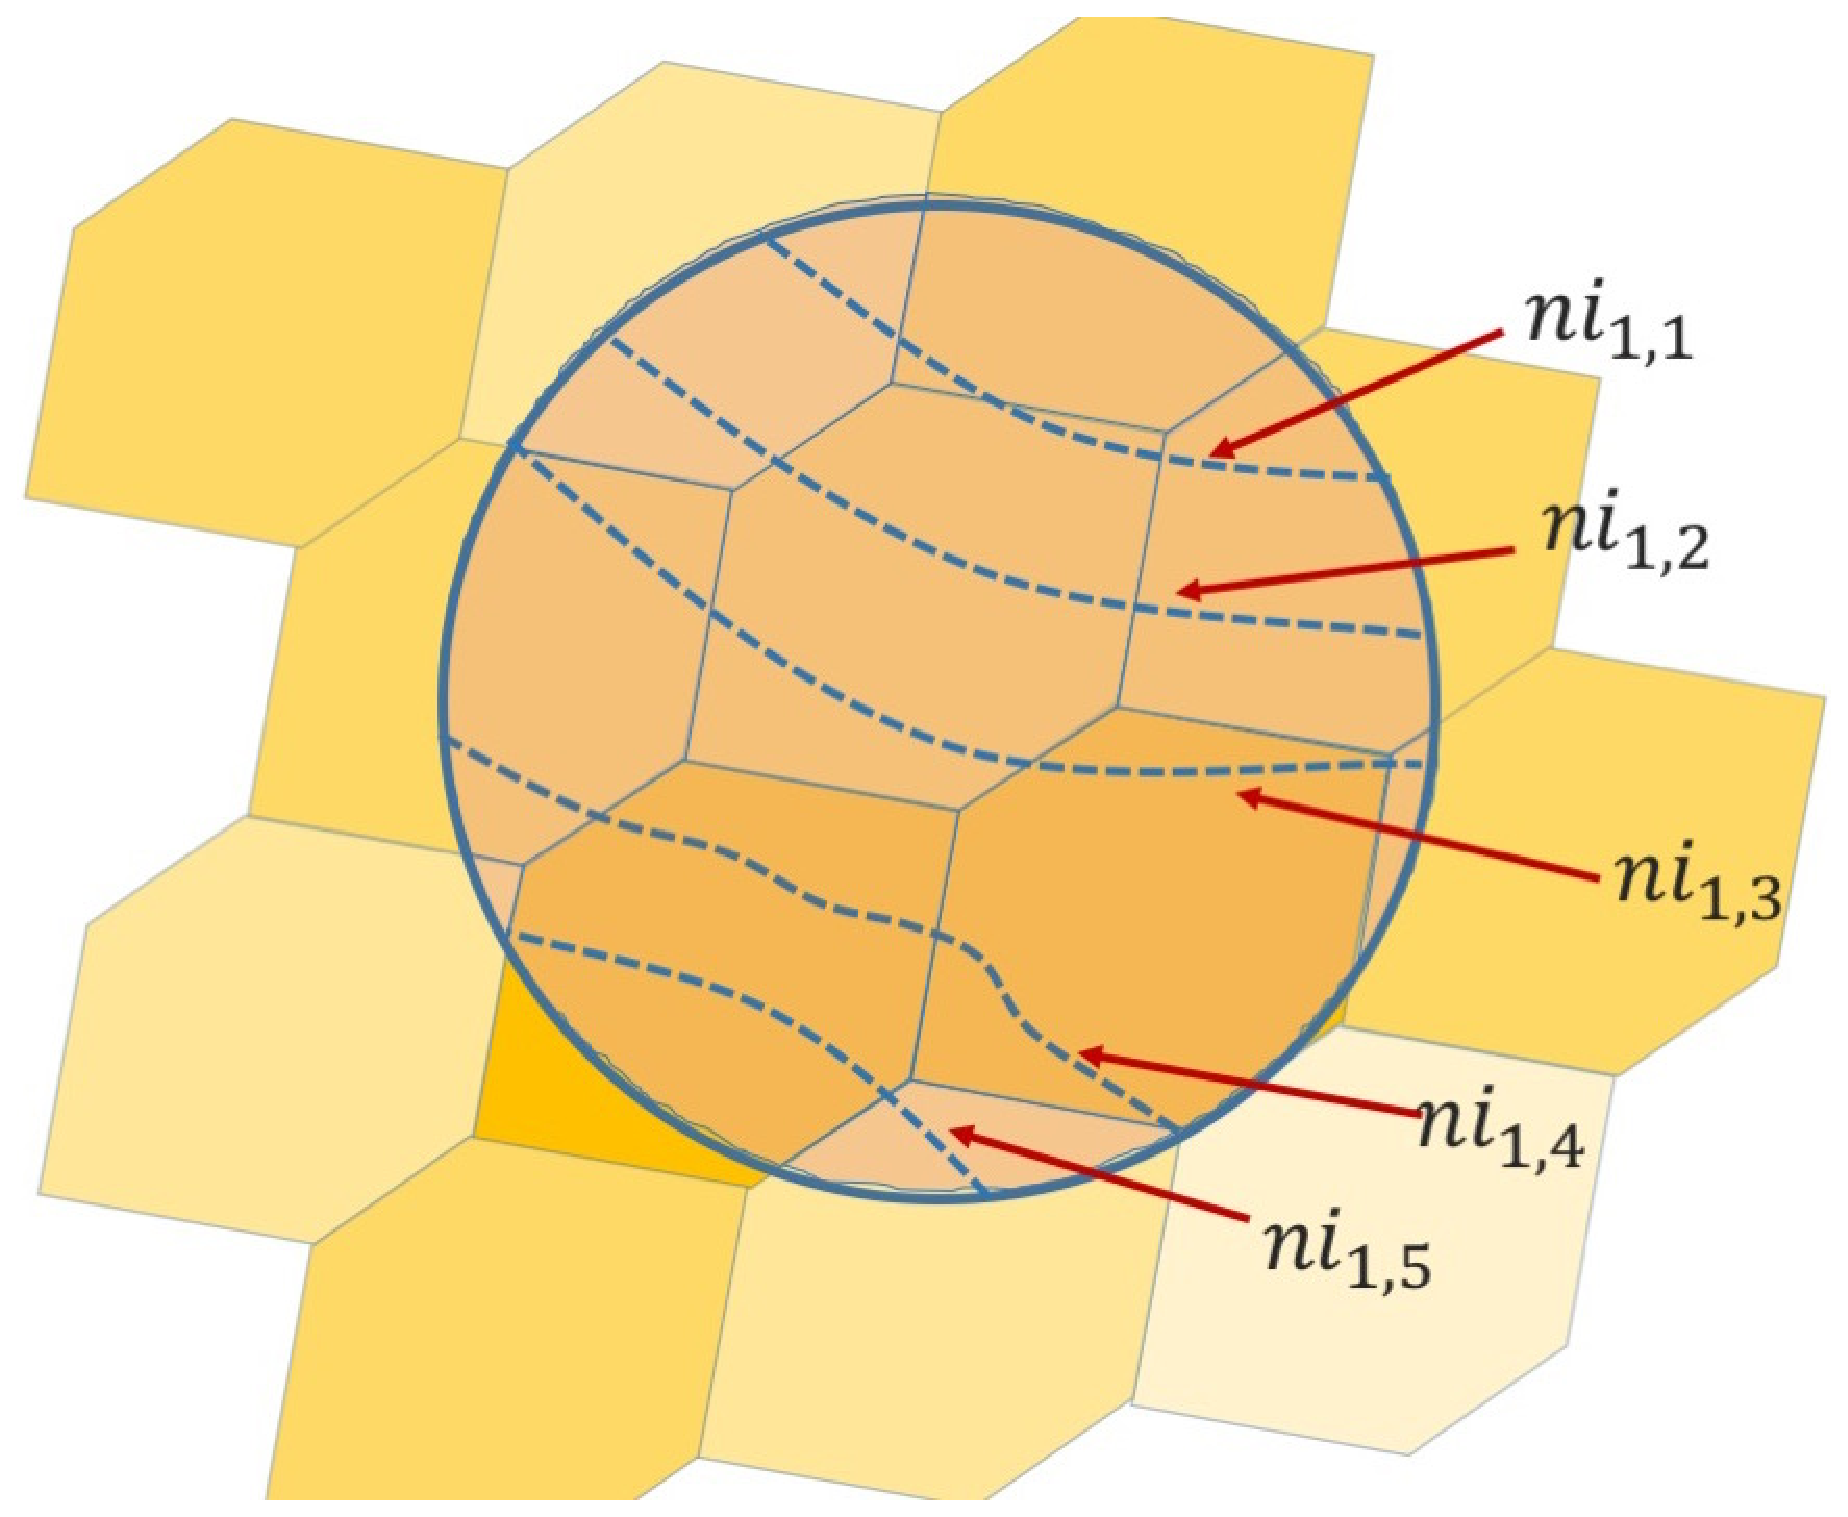
\includegraphics[width=1\textwidth]{images/ni}
			\caption{Le linee in blu tratteggiate rappresentano le nearest isoipse $ni_{1,o}$.}
			\label{NearestIso}
		\end{minipage}
		\hspace{0.05\linewidth}
		\begin{minipage}[t]{0.45\linewidth}
			\centering
			\includegraphics[width=1\textwidth]{images/zf}
			\caption{ 
				I quattro poligoni in blu con i contorni gialli rappresentano le $zf_{1,1,t}$ relative alla nearest zone $nz_{1,1}$. }
			\label{zf}
		\end{minipage}
	\end{figure}
	
	\item \textbf{ $czf_{i,j,t}$ (Centroid of $zf_{i,j,t})$} corrisponde al centro di massa dello zone fragment $zf_{i,j,t}$ la cui posizione è descritta dalle sue coordinate geografiche date dalla coppia $(czfx_{i,j,t}, czfy_{i,j,t})$ (Figura \ref{czf}).
	
	\begin{figure}[h]
		\centering
		\includegraphics[width=0.45\textwidth]{images/czf}
		\caption{
			I pallini bianchi rappresentano i $czf_{1,1,t}$ ovvero i centri di massa delle zone fragments $zf_{1,1,t}$ della (Figura \ref{zf}) .}
		\label{czf}
	\end{figure}
	
	\item \textbf{$ \mathcal{LR}_i $} (\textbf{LinearRegressions}) $ = \{lr_{i,j}(i=1,..,\mathbf{card}(\mathcal{B})),(j=1,..,\mathbf{card}(\mathcal{NZ}_i)\} | lr_{i,j} $ rappresenta la retta di regressione lineare della \textit{Nearest Zone} $nz_{i,j}$. Nel caso specifico $lr_{i,j} $ rappresenta la retta passante per il centro di massa $cnz_{i,j}$ della nearest zone $nz_{i,j}$ con coefficiente angolare \textit{m} tale che, dati i centri di massa ($czfx_{i,j,t}, czfy_{i,j,t}$)  delle zone fragment $zf_{i,j,t}$,  sia minima la somma dei quadrati dei loro scarti (Figura \ref{linear_regression}). Matematicamente essa è descritta come segue:\\
	\\
	l'equazione (\ref{eq:retta_passante_per}) rappresenta la retta passante per il centro di massa $cnz_{i,j}$ rappresentata in Figura \ref{linear_regression}
	\begin{equation}\label{eq:retta_passante_per}
		y - cnzy_{i,j} = m(x-cnzx_{i,j})
	\end{equation}
	
	per la quale dati $t$ punti ($czfx_{i,j,t}, czfy_{i,j,t}$) risulta minima la somma dei quadrati degli scarti:
	\begin{equation}\label{eq:somma_degli_scarti}
		S(m, q) = \sum_{i=0}^n (m*czfx_{j,t} + q - czfy_{j,t})^2 
	\end{equation}
	\begin{equation}
		\textnormal{ove}\: q = cnzy_{i,j} - m*cnzx_{i,j}
	\end{equation}
	Questo concetto matematico sarà utilizzato per stimare la direzione di caduta della frana relativa alla $nz_{i,j}$ Figura \ref{linear_regression}.
		
	\newpage
	\item \textit{$BuildingBuffer_i$} rappresenta l'area circostante l'edificio $b_i$ e ne approssima l'estensione. E' definita come la circonferenza centrata su $b_i$ di raggio $l$ dove $l<<r $ con $r$ raggio del \textit{$HazardArea_i$} (Figura \ref{buildingimpactfactor}).
	
	\begin{figure}[h]
		\centering
		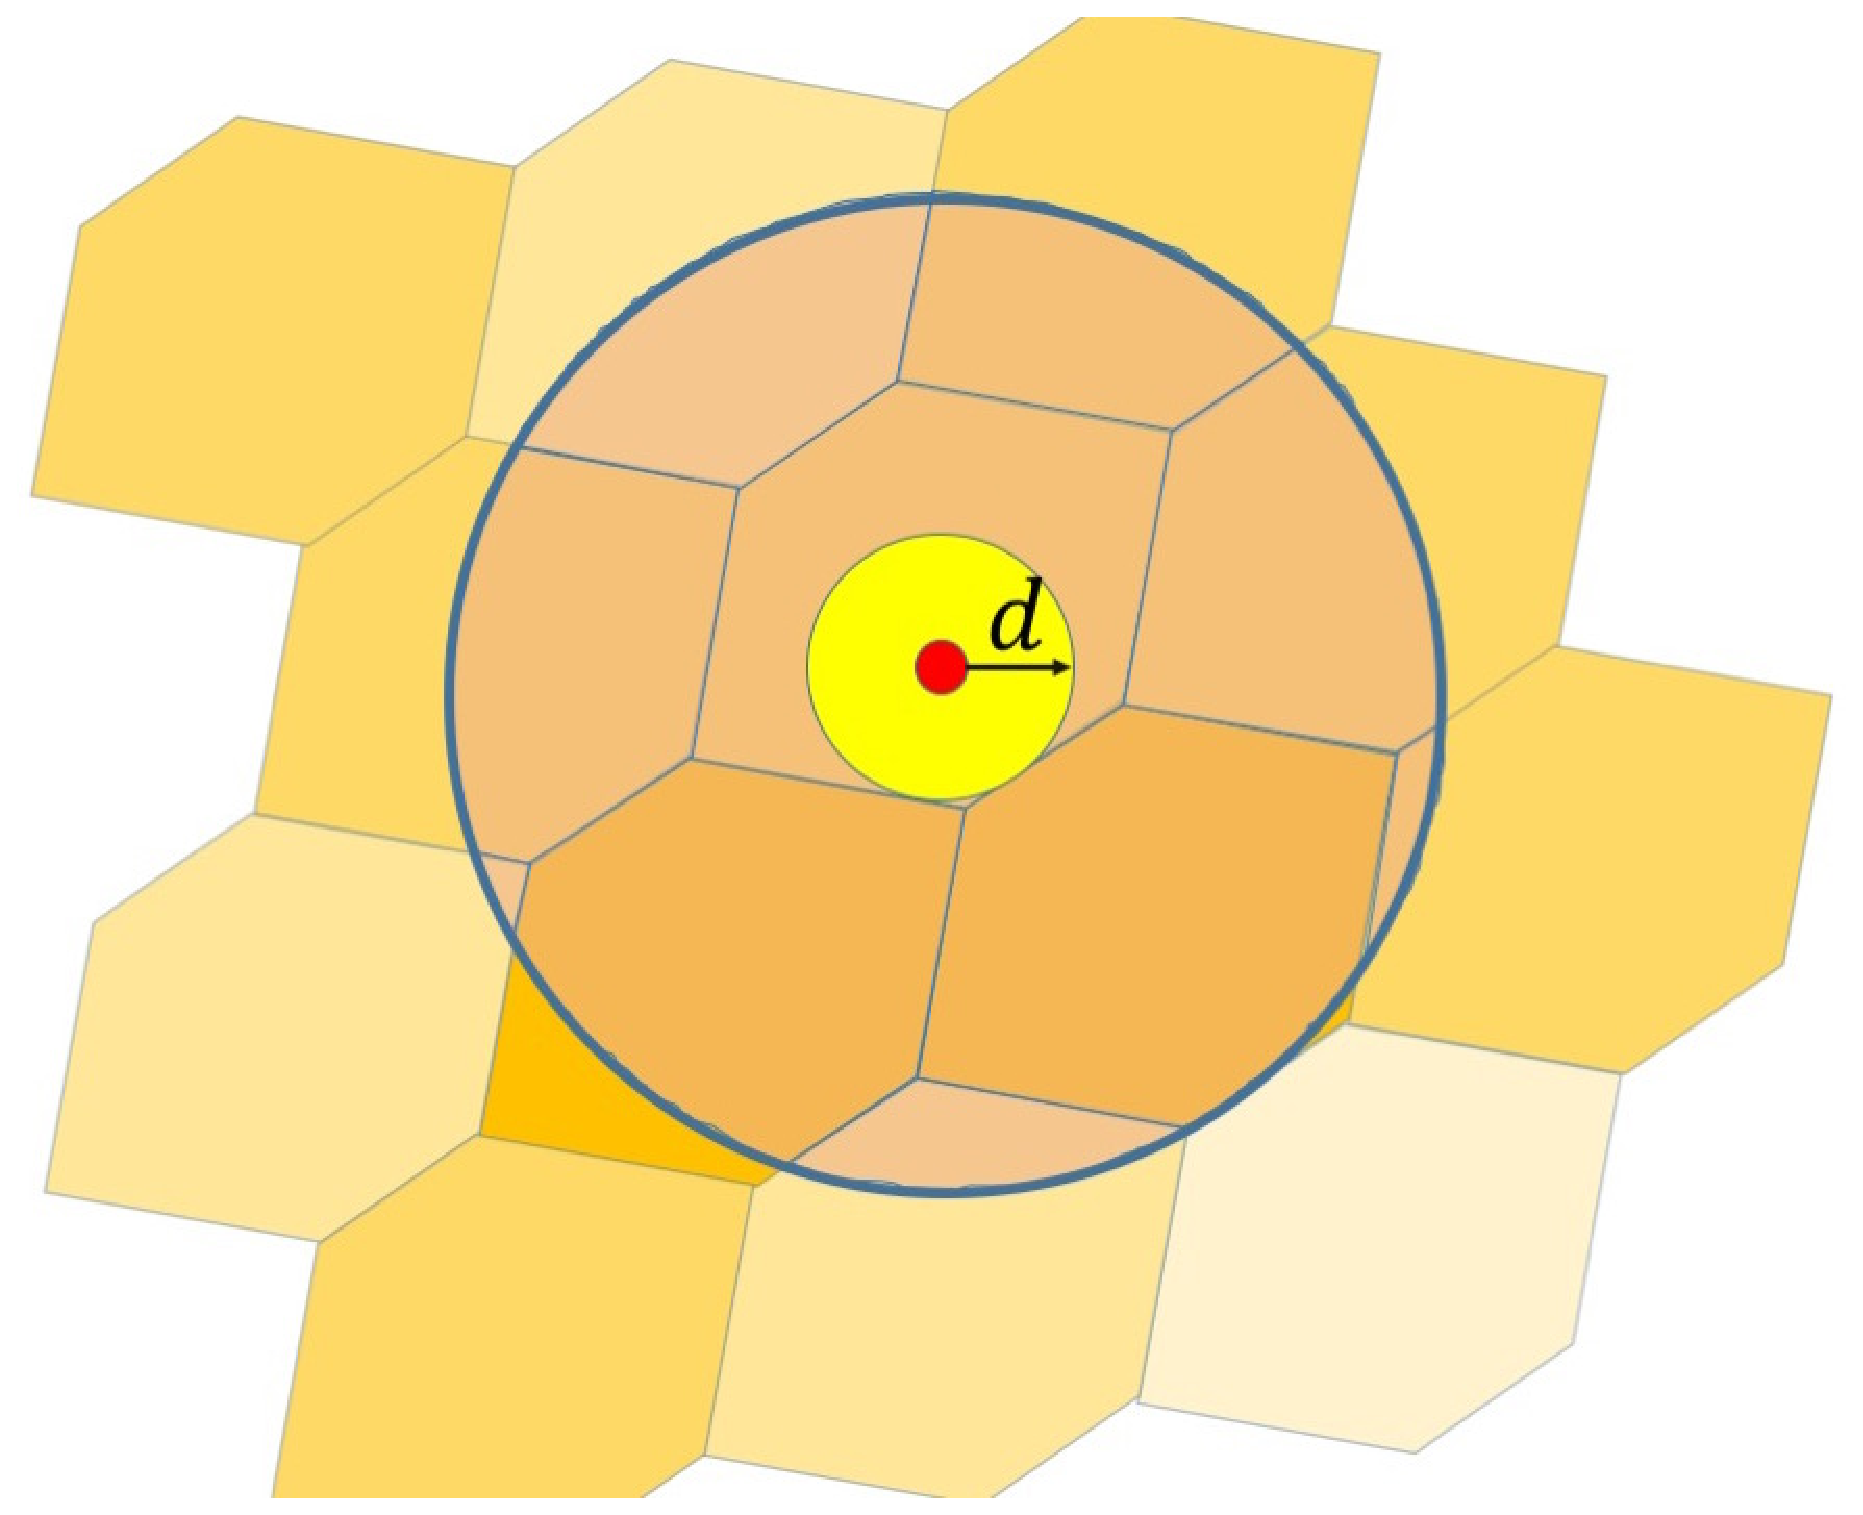
\includegraphics[width=0.5\textwidth]{images/buildingimpactfactor}
		\caption{L'area di colore giallo intorno all'edificio rappresenta il $BuildingBuffer_i$ di raggio $l$.}
		\label{buildingimpactfactor}
	\end{figure}
	
	\item \label{last_enum} \textbf{$EXP$ (Exposure)} $ = \{exp_i(i=1,..,\mathbf{card}(\mathcal{B})) | exp_i $ è il valore di \textit{exposure} del building i-esimo. Per \textit{exposure} si intende il valore numerico che indica quanto il building è esposto al rischio frana, 
	rappresentato dalla tupla <\textit{ID}, \textit{description}, \textit{position}, \textit{exposure}> 
	
			\begin{figure}[h]
		\centering
		\includegraphics[width=0.6\textwidth]{images/linear_regression1}
		\caption{La retta di regressione lineare $lr_{i,j}$ di colore celeste, minimizza la distanza (rappresentata con la linea verde chiaro) tra i punti (in questo caso gli $czf_{i,j,t}$) e la retta stessa.}
		\label{linear_regression1}
	\end{figure}
	\newpage
	\begin{figure}[t!]
		\centering
		\includegraphics[width=0.45\textwidth]{images/linear_regression2}
		\caption{\textcolor{red}{L'immagine ha bisogno del testo specifico alla caption} Rappresentazione della retta di regressione lineare di $nz_{1,1}$. Si nota in figura che $lr_{1,1}$ passa per il centro di massa della \textit{Nearest Zone}}.
		\label{linear_regression}
	\end{figure}
	
\end{enumerate}
 % Notazione
% Chapter 3

\chapter{Metodo per il ranking delle stazioni ferroviarie} % Chapter title

\label{ch:mathtest} % For referencing the chapter elsewhere, use \autoref{ch:mathtest}

Il fine del metodo che ci si accinge a descrivere è valutare il livello di rischio frana (Exposure) al quale potrebbero essere soggetti un insieme di assets. Con tale valutazione si potrà creare una graduatoria degli assets più a rischio di una determinata zona (\textit{GeoArea}) e potrà essere di supporto agli enti responsabili di manutenzione o controllo della zona stessa. Il metodo che verrà sviluppato tiene a mente tutte le considerazioni presentate nella introduzione, da cui è emerso che oltre alla ripidità del pendio e allo spazio percorso dalla frana è fondamentale anche la traiettoria seguita. Quest'ultima è alla base del metodo ed è stato il principale elemento di studio. Per un'analisi approfondita di questi aspetti sono sono state introdotte le curve di livello ($\mathcal{I}$). Inoltre il territorio preso in considerazione (\textit{GeoArea}), dove sono dislocati gli assets strategici ($\mathcal{B}$), è stato suddiviso in piccole particelle di terreno ($\mathcal{Z}$) dalle quali può aver origine una frana se si verificano determinate condizioni che andremo a definire.


\begin{figure}[h]
	\centering
	\includegraphics[width=0.7\textwidth]{images/raggio_di_azione_frana}
	\caption{Due assets che si trovano nei pressi di un pendio. Entrambi hanno la propria \textit{HazardArea} di raggio $r$, di cui quella dell'edificio in rosso comprende il punto di distacco del masso. Quindi l'edificio si trova in una zona pericolosa, al contrario di quello di colore verde. }
	\label{raggio_azione_frana}
\end{figure}

Il metodo calcola per ogni asset $b_i$, il relativo valore di exposure. Ricordando dall'introduzione che una frana può estendersi per una distanza notevole ma pur sempre limitata (Figure \ref{raggio_azione_frana}), sembra logico limitare l'area di studio alla sola ($HazardArea_i$). L'analisi che segue quindi interesserà le sole Zones $\mathcal{Z}$ all'interno di tale area, ovvero le particelle appartenenti all'insieme $\mathcal{NZ}_i$ (\textit{Nearest Zones} di $b_i$) (Figura \ref{landslide0}).
Come detto in precedenza, elemento fondamentale alla base del metodo è la  traiettoria di frana. Il metodo infatti stima tale traiettoria per ognuna delle \textit{Nearest Zones} $nz_{i,j} \in \mathcal{NZ}_i$ dunque è indispensabile considerare le curve di livello  (Figura \ref{landslide1}). 

\begin{figure}[h]
	\hspace{0.05\linewidth}
	\begin{minipage}[t]{0.4\linewidth}
		\centering
		\includegraphics[width=\textwidth]{images/landslide0}
		\caption{In giallo è evidenziata una delle Nearest Zone dell'edificio di colore rosso.}
		\label{landslide0}
	\end{minipage}
	\hspace{0.05\linewidth}
	\begin{minipage}[t]{0.4\linewidth}
		\centering
		\includegraphics[width=\textwidth]{images/landslide1}
		\caption{Impiego delle curve di livello per il calcolo della traiettoria della frana}
		\label{landslide1}
	\end{minipage}
\end{figure}

Naturalmente le sole curve di livello di interesse alla $nz_{i,j}$ sono quelle che intersecano la $HazardArea_i$, ovvero le (Nearest Isoipses) $\mathcal{NI}_i$.
Queste ultime vengono utilizzate per determinare la distribuzione delle masse all'interno della particella di terreno $nz_{i,j}$. Pertanto esse verranno utilizzate per frazionare la $nz_{i,j}$  in frammenti $zf_{i,j,t}$. I centri di massa ($czf_{i,j,t}$) di tali frammenti sono alla base del calcolo della regressione lineare. Dal calcolo della regressione lineare otteniamo la retta ($lr_{i,j}$) che stima appunto la traiettoria di frana della particella $nz_{i,j}$. 

A questo punto, ricavata la retta che stima la traiettoria di frana $lr_{i,j}$ della particella $nz_{i,j}$, bisogna determinare se la presunta frana di tale particella "impatta" o meno sull'edificio $b_i$ oggetto di analisi. Per poter comprendere appieno cosa si intende per "impatto" è necessario definire le seguenti notazioni:

\begin{enumerate}
	\setcounter{enumi}{13}
	\item \textbf{$ \mathcal{BLR}_i $} (\textbf{Buffered Linear Regressions}) $= \{blr_{i,j}(i=1,..,\mathbf{card}(\mathcal{B})),(j=1,..,\mathbf{card}(\mathcal{NZ}_i)\}$ | $\forall lr_{i,j} \in $ \textbf{$ \mathcal{LR}_i $} si ha che $blr_{i,j}$ è la geometria risultante dalla \textit{LineBuffering} di $lr_{i,j}$. $blr_{i,j}$ rappresenta quella che potrebbe essere la scia della frana di $nz_{i,j}$ alla quale ci si riferisce. Ovvero identifica l'area che tale frana mette a rischio. 
	Per una migliore comprensione riferirsi alla (Figura \ref{buffer_regression})
	
	\begin{figure}[h]
		\centering
		\includegraphics[width=0.5\textwidth]{images/buffer_rect}
		\caption{La \textbf{Buffered Linear Regression} $blr_{i,j}$ ottenuta dalla \textit{LineBuffering} della retta di regressione lineare $lr_{i,j}$. Essa rappresenta l'area attorno alla retta entro una distanza $d$ dalla stessa.}
		\label{buffer_regression}
	\end{figure}
	
	\item \textbf{$ \mathcal{LS}_i $} (\textbf{LandSlides}) $ = \{ls_{i,j}(i=1,..,\mathbf{card}(\mathcal{B})),(j=1,..,\mathbf{card}(\mathcal{LS}_i)\}$ con $\mathcal{LS}_i \subseteq \mathcal{BLR}_i$  sottoinsieme | $\mathcal{LS}_i = (\mathcal{BLR}_i  \cap BuildingBuffer_i)	\not= \emptyset $.
	Con parole esplicite, gli elementi dell'insieme $ \mathcal{LS}_i $ sono	le sole $blr_{i,j}$ che intersecano il \textit{BuildingBuffer$_i$}. Nello specifico, le sole frane che "impattano" l'edificio $b_i$ (Figura \ref{landslides}).
	
	\begin{figure}[h]
		\centering
		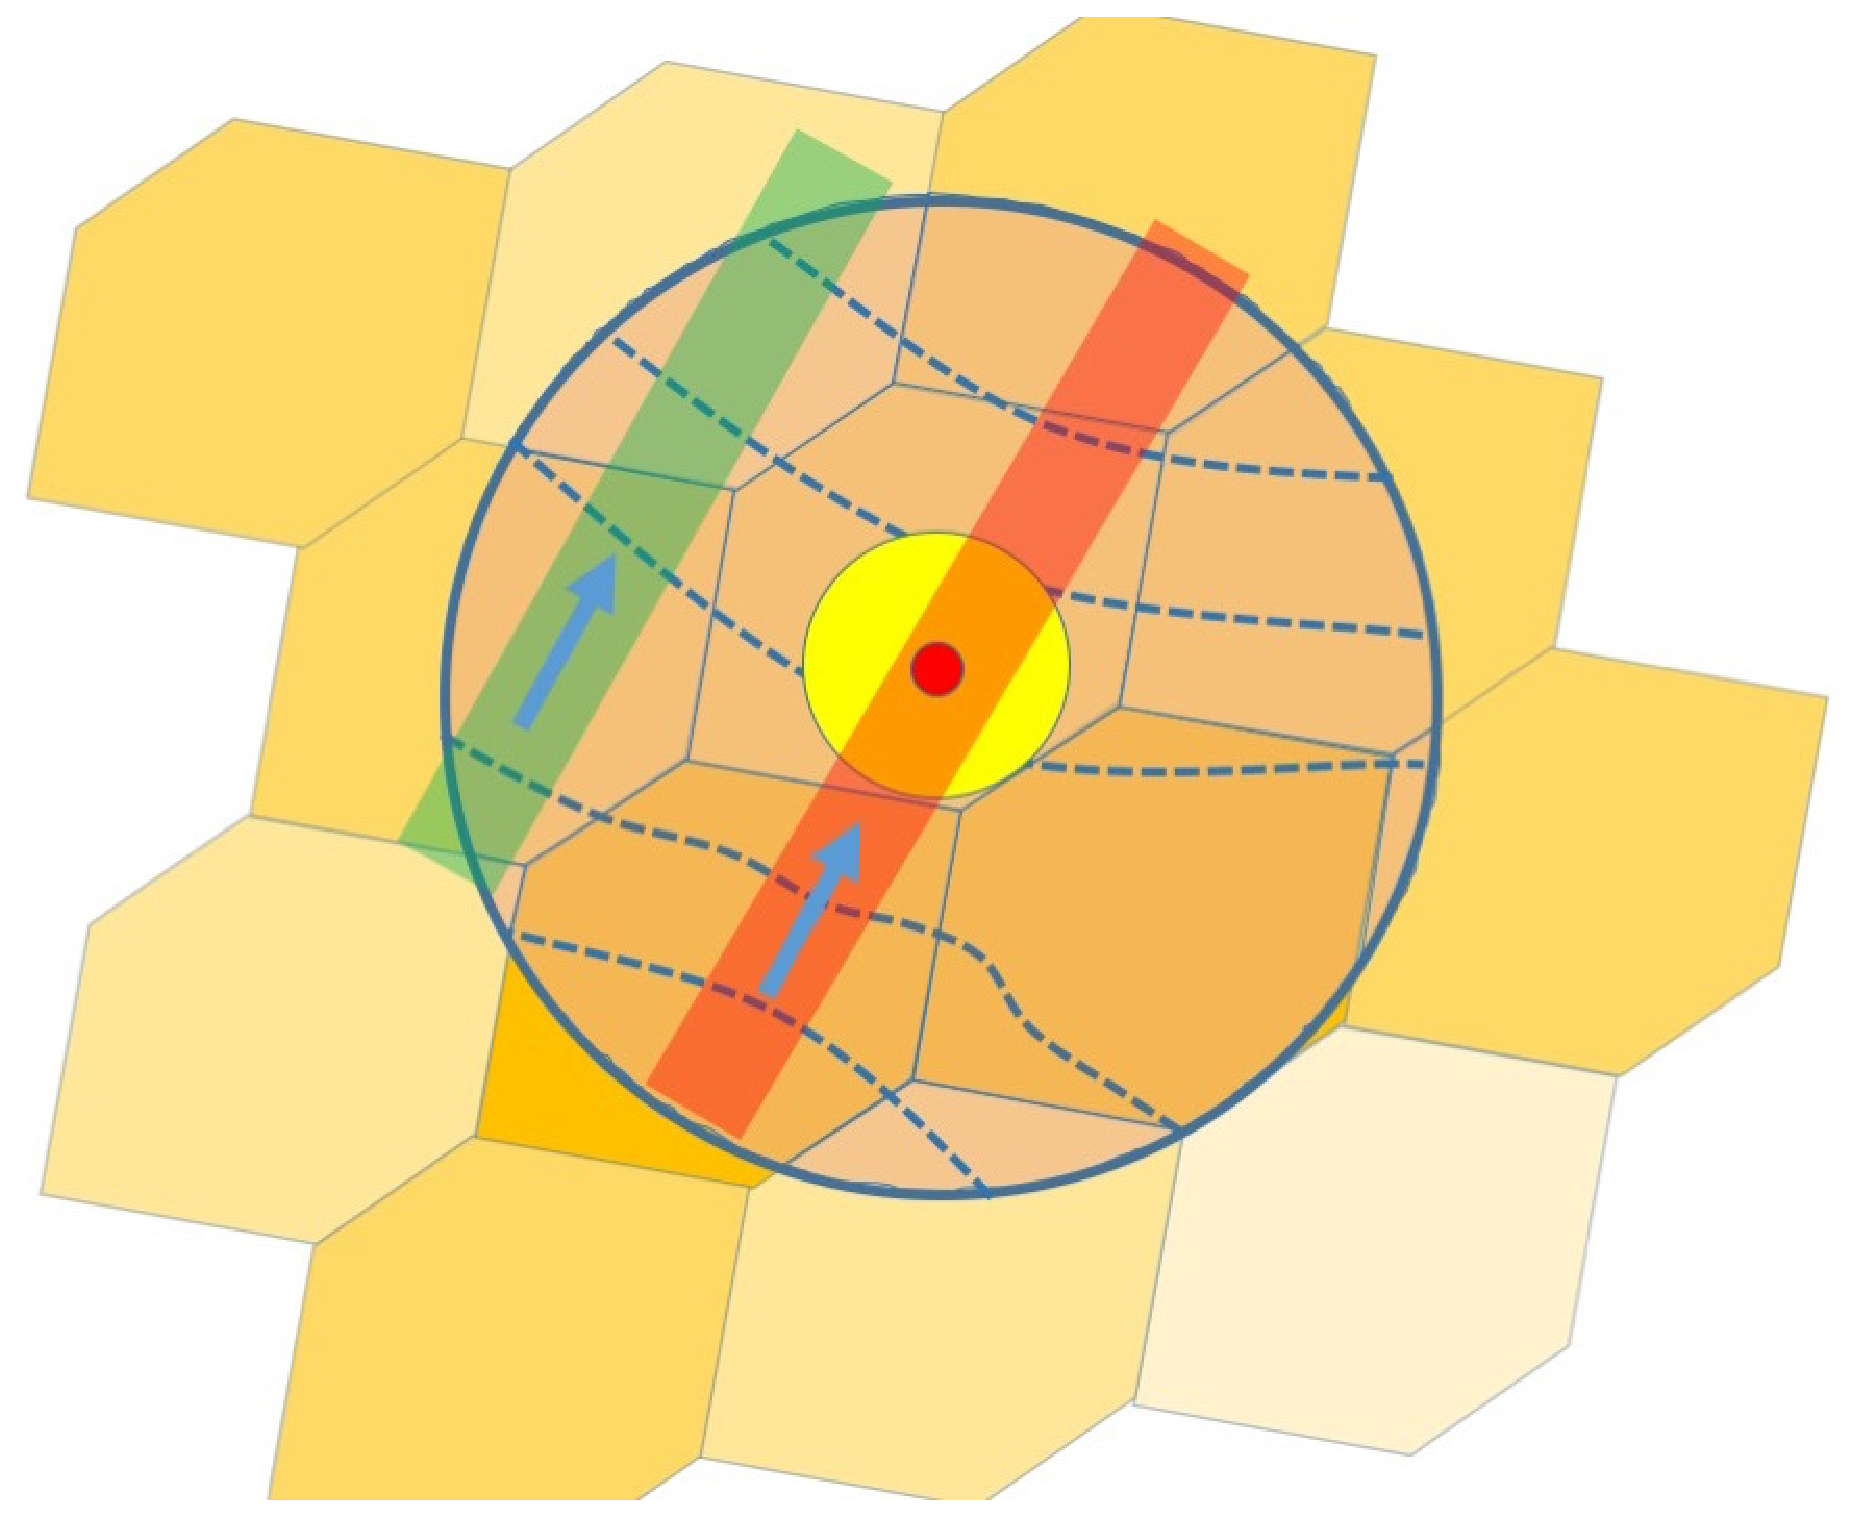
\includegraphics[width=0.4\textwidth]{images/landslides}
		\caption{Il rettangolo verde rappresenta una \textit{Buffered Linear Regression} che non costituisce un pericolo per l'edificio. In rosso invece è stata raffigurata una \textit{Buffered Linear Regression} che impatta sull'edificio pertanto essa appartiene all'insieme $\mathcal{LS}_i$ del relativo building $b_i$.}
	\label{landslides}
	\end{figure}
	

%\begin{figure}[h]
%	\hspace{0.05\linewidth}
%	\begin{minipage}[t]{0.4\linewidth}
%		\centering
%		\includegraphics[width=\textwidth]{images/landslide2}
%		\caption{Modificare immagne cn landslide che pasa affianco alla stazione}
%		\label{landslide2}
%	\end{minipage}
%	\hspace{0.05\linewidth}
%	\begin{minipage}[t]{0.4\linewidth}
%		\centering
%		\includegraphics[width=\textwidth]{images/landslide3}
%			\caption{textcolor{red}{Da scrivere}}
%		\label{landslide3}
%	\end{minipage}
%\end{figure}
	
\end{enumerate}

Avendo definito la nozione di frana che "impatta" sull'edificio $b_i$, rimane da tener conto di un altro fattore determinante, ossia l'entità di tale "impatto". Una \textit{LandSlide} di fatto può "impattare" su un edificio in modo totale o parziale e di conseguenza influire diversamente sul valore di exposure della stessa. Introduciamo pertanto la notazione di \textit{Impact Factor}

\begin{enumerate}
	\setcounter{enumi}{15}
	
	\item \textbf{$IFls_{i,j}$} (\textbf{Impact Factor}) è un valore percentuale $\in(0,1]$ che esprime l'entità dell'impatto della $ls_{i,j}$ sull'edificio $b_i$. Essa corrisponde al rapporto tra l'area della $ls_{i,j} \cap BuildingBuffer_i$ e l'area del $BuildingBuffer_i$ (Equazione \ref{eq:impactfactor}). Un valore di $IFls_{i,j}=1$ equivale a dire che la frana impatta in modo totale sull'edificio. Da tenere conto che un valore pari a 0 non è possibile essendo l'insieme $ \mathcal{LS}_i $ quello delle sole frane che impattano su $b_i$.
	
	\begin{equation}\label{eq:impactfactor}
	ImpactFactor=\frac{Area(BuildingBuffer_i \cap ls_{i,j})}{Area(BuildingBuffer_i)}
	\end{equation}
	
	In (Figura \ref{impact_factor}) vediamo da due diverse prospettive i casi di impatto di una \textit{LandSlide}.
	
	\begin{figure}[h]
		\centering
		\includegraphics[width=0.9\textwidth]{images/landslide5}
		\caption{A sinistra il caso di impatto totale a cui corrisponderà una \textit{Impact Factor} pari a 1. A destra il caso di impatto parziale a cui corrisponderà una \textit{Impact Factor} $<1$  }
		\label{impact_factor}
	\end{figure}
	
\end{enumerate}

\newpage 
A questo punto si ha tutto il necessario per poter calcolare l'exposure dell'edificio $b_i$ che naturalmente terrà conto di tutti i fattori descritti in precedenza. Quindi, per ogni $b_i$ l'Exposure sarà calcolata come la somma dei valori di exposure parziali $Pexp_{i,j}$ (Definizione \ref{Pexp}) derivanti dai contributi delle sole \textit{NearestZones} le quali \textit{LandSlides} $ls_{i,j}$ impattano sull'edificio stesso.
Definiamo tali zone come \textit{LandSlideZones} (Definizione \ref{LSZ})

\begin{enumerate}
	\setcounter{enumi}{16}

	\item \label{LSZ} \textbf{$ \mathcal{LSZ}_i $ (LandSlideZones)} $ = \{lsz_{i,j}(i=1,..,\mathbf{card}(\mathcal{B})),(j=1,..,\mathbf{card}(\mathcal{LSZ}_i)\}$ con $\mathcal{LSZ}_i \subseteq \mathcal{NZ}_i$ | $\mathcal{LSZ}_i$ 
	è l'insieme delle sole $nz_{i,j}$ aventi $ls_{i,j}$ che impattano sull'edificio $b_i$. 
	Con parole più esplicite, $lsz_{i,j}$ è la Zone relativa alla \textit{LandSlide} $ls_{i,j}$. 
	Tenendo presente che $\mathcal{LSZ}_i$ è un sottoinsieme di $\mathcal{NZ}_i$, l'elemento $lsz_{i,j}$  è descritto dalla medesima tupla <\textit{ID}, \textit{boundary}, \textit{$Sz_k$}> di $nz_{i,j}$ . 
	
	\item \label{Pexp} $pexp_{i,j}$ \textbf{(Partial Exposure)} | $ pexp_{i,j}(i=1,..,\mathbf{card}(\mathcal{B})),(j=1,..,\mathbf{card}(\mathcal{LSZ}_i)$ è il valore di exposure parziale con cui la \textit{LandSlideZone} $lsz_{i,j}$ influisce sull'edificio $b_i$. Tale valore dipende dal valore di $Sz_k$ della $lsz_{i,j}$ , dall'area della zone stessa, e dal \textit{Impact Factor} $IFls_{i,j}$ della relativa \textit{LandSlide} sull'edificio $b_i$. Matematicamente $pexp_{i,j}$ è descritta dalla (Equazione \ref{eq:exposure2}). Nel caso singolare in cui ($lsz_{i,j}$ contiene $b_i==true$), ovvero quando si sta calcolando la \textit{Partial Exposure} della specifica \textit{LandSlideZone} che contiene $b_i$, la relativa $pexp_{i,j}$ viene calcolata imponendo la $IFls_{i,j}=1$ (Equazione \ref{eq:exposure3})  
	\\
	\begin{enumerate}
		\item[$\bullet$] Se $lsz_{i,j}$ contiene $b_i$
		\begin{equation}\label{eq:exposure2}
		pexp_{i,j} =(Area)*(Sz_{k}) * IFls_{i,j}
		\end{equation}
		
		\item[$\bullet$] Altrimenti
		\begin{equation}\label{eq:exposure3}
		pexp_{i,j} =(Area)*(Sz_{k})
		\end{equation}
	\end{enumerate}

	{Con $j$ fissato, "Area" e "$Sz_k$" sono la rispettiva Area e valore $Sz_k$ della relativa $lsz_{i,j}$.}
	
\end{enumerate}

Pertanto abbiamo che l'exposure totale risulta essere definita dalla seguente equazione

\begin{equation}\label{eq:exposure1}
exp_i =\sum_{j=1}^n pexp_{i,j}
\end{equation}

ove n=$\mathbf{card}(\mathcal{LSZ}_i)$
\bigbreak

Infine il metodo restituirà per ogni edificio $b_i$ della \textit{GeoArea} un valore di exposure $exp_i$.






 %Metodo
% Chapter X

\chapter{Pseudo-codice del metodo} % Chapter title

\label{ch:name} % For referencing the chapter elsewhere, use \autoref{ch:name} 
Di seguito verrà proposto lo pseudo-codice dell'algoritmo per il calcolo dell'esposizione al rischio di frana di un \textit{Building}. L'algoritmo qui proposto utilizza un approccio funzionale alla risoluzione del problema: Permette infatti di separare la problematica del calcolo dell'exposure in sotto-problemi atomici. Inoltre ciò semplifica notevolmente la scrittura e la comprensione dello stesso.


% Algorithm

\begin{algorithm}[H]
	
	\SetKwData{Left}{left}\SetKwData{This}{this}\SetKwData{Up}{up}
	\SetKwFunction{Union}{Union}\SetKwFunction{FindCompre
		ss}{FindCompress}
	\SetKwInOut{Input}{Input}\SetKwInOut{Output}{Output}
	
	\IncMargin{1em}
	\Input{$b_i$,$\mathcal{Z}$,$\mathcal{I}$,r,d,l}
	\Output{$exp_i$} 
	\caption{Exposure ($b_i$,$\mathcal{Z}$,$\mathcal{I}$,r,d,l)}
	\label{alg:0}
	\BlankLine
	
	\SetAlgoNoLine
	$ \mathcal{NZ}_i \leftarrow$ NearestZonesFinder($\mathcal{Z},b_i$,r); \\
	$ \mathcal{NI}_i \leftarrow$ NearestIsoipseFinder($\mathcal{I},b_i,r$); \\
	$ \mathcal{ZF}_i \leftarrow$ ZoneFragmentFinder($b_i , \mathcal{NI}_i , \mathcal{NZ}_i $);  \\
	$ \mathcal{BLR}_i \leftarrow $ BufferedLinearRegressionFinder($b_i,\mathcal{NZ}_i,\mathcal{ZF}_i,\mathcal{NZ}_i$,d); \\
	$ \mathcal{LS}_i \leftarrow $ LandSlideFinder($b_i , \mathcal{LR}_i $); \\
	$ exp_i \leftarrow$ ContributionOfLandSlide($b_i ,l, \mathcal{LS}_i $);\\
	return $ exp_i $;
	
	
\end{algorithm}
La funzione Exposure ($b_i$) elenca i passi fondamentali per poter calcolare il  valore d'exposure dell'edificio $b_i$. Di seguito verranno esposti i dettagli di tutte le funzioni richiamate.

\begin{algorithm}[H]
	
	\SetKwData{Left}{left}
	\SetKwData{This}{this}
	\SetKwData{Up}{up}
	\SetKwFunction{Union}{Union}
	\SetKwFunction{FindCompress}{FindCompress}
	\SetKwInOut{Input}{Input}
	\SetKwInOut{Output}{Output}
	\IncMargin{1em}
	\Input{$\mathcal{Z}$,$b_i$,r}
	\Output{$\mathcal{NZ}_i $} 
	\caption{NearestZonesFinder($\mathcal{Z},b_i$,r)}
	\label{alg:1}
	\BlankLine
	\SetAlgoNoLine
	$ HazardArea_i  \leftarrow $ \textbf{ST\_Buffer($b_i$,r)} ; \\ 
	$ \mathcal{NZ}_i  \leftarrow $ $HazardArea_i \cap \mathcal{Z}$; \\
	return $\mathcal{NZ}_i$;
	
\end{algorithm}

\begin{enumerate}
	\item Crea un buffer ($ HazardArea_i $) di raggio r intorno all'edificio $b_i$
	\item Interseca tale buffer con le zone dell’insieme $\mathcal{Z}$. Il risultato è l’insieme contenente le sole zone con intersezione non vuota con il buffer costruito, ovvero l’insieme  $\mathcal{NZ}_i$
\end{enumerate}

\begin{algorithm}[H]
	
	\SetKwData{Left}{left}\SetKwData{This}{this}\SetKwData{Up}{up}
	\SetKwFunction{Union}{Union}\SetKwFunction{FindCompress}{FindCompress}
	\SetKwInOut{Input}{Input}\SetKwInOut{Output}{Output}
	
	\IncMargin{1em}
	\Input{$\mathcal{I},b_i,r$}
	\Output{$ \mathcal{NI}_i $} 
	\caption{NearestIsoipseFinder($\mathcal{I},b_i,r$)}
	\label{alg:two}
	\BlankLine
	\SetAlgoNoLine
	$  HazardArea_i   \leftarrow $ \textbf{ST\_Buffer($b_i$,r)}; \\
	$ \mathcal{NI}_i \leftarrow $ $HazardArea_i \cap \mathcal{I} $; \\
	return $\mathcal{NI}_i;$
\end{algorithm}
\begin{enumerate}
	\item Crea un buffer ($ HazardArea_i $) di raggio r intorno all'edificio $b_i$
	\item Interseca tale buffer con le isoipse dell’insieme $\mathcal{I}$. Il risultato è l’insieme contenente le sole isoipse con intersezione non vuota con il buffer costruito, ovvero l’insieme  $\mathcal{NI}_i$
\end{enumerate}

\begin{algorithm}[H]
	
	\SetKwData{Left}{left}\SetKwData{This}{this}\SetKwData{Up}{up}
	\SetKwFunction{Union}{Union}\SetKwFunction{FindCompress}{FindCompress}
	\SetKwInOut{Input}{Input}\SetKwInOut{Output}{Output}
	\IncMargin{1em}
	\Input{$b_i,\mathcal{NZ}_i,\mathcal{NI}_i$}
	\Output{$\mathcal{ZF}_i$} 
	\caption{ZoneFragmentFinder($b_i,\mathcal{NZ}_i,\mathcal{NI}_i$)}
	\label{alg:four}
	\BlankLine
	\SetAlgoNoLine
	$\mathcal{ZF}_i \leftarrow$ \O \\
	\For{ each $nz_{i,j}$ in $\mathcal{NZ}_i$  }{
		$Tf$ $\leftarrow$ \O  ; \\
		$Ti$ $\leftarrow nz_{i,j} \cap \mathcal{NI}_i $; \\
		$Tf$ $\leftarrow$ $Tf$ + \textbf{ST\_split($nz_{i,j}$} , $Ti$ [ 1 ] ) ; \\
		$Ti$ $\leftarrow$ $Ti$ - \{ $Ti$ [ 1 ] \}; \\
		\While {Tf is not empty } {
			$Ci$ $\leftarrow $ $Tf$ [ 1 ] $\cap$ $Ti$  ;\\
			\If {Ci is not empty }{
				$Tf$ $\leftarrow$ $Tf$ + \textbf{ST\_split}( $Tf$ [ 1 ], $Ci$ [ 1 ] ) ;\\
				$Tf$ $\leftarrow$ $Tf$ - \{ $Tf$ [ 1 ] \} ;\\
				$Ti$ $\leftarrow$ $Ti$ - \{ $Ci$[ 1 ] \} ;\\
			}
			\Else { 
				$\mathcal{ZF}_i$ $\leftarrow$ $\mathcal{ZF}_i$ + \{ $Tf$ [ 1 ] \} ;\\
				$Tf$ $\leftarrow$ $Tf$ - \{ $Tf$ [ 1 ] \} ;\\
				
			}
		}
	}
	
	return $\mathcal{ZF}_i;$
\end{algorithm}
La funzione ZoneFragmentFinder($b_i$) esegue una multi-split tra $\mathcal{NZ}_i$ e i frammenti di isoipse contenuti nell'insieme $\mathcal{NI}_i$.
Il risultato di detta operazione è descritto in figura \ref{zf}.
\begin{enumerate}
	\item Si inizializza l'insieme $\mathcal{ZF}_i$.
	\item Per ogni $nz_i$ contenuto nell'insieme $\mathcal{NZ}_i$ si attiva l'esecuzione del ciclo. L'indice $i$ è bloccato sul building $i$-esimo mentre la $j$ si muove nell'intervalo (1,..,$\mathbf{card}(\mathcal{NZ}_i)$).
	\item Si inizializza l'insieme $Tf$ (Temp\_fragment) che conterrà i frammenti intermedi prossimi candidati ad essere delle \textit{Zone Fragment} nel caso non ci siano ulteriori split possibili con esse.
	\item Assegnazione all'insieme $Ti$(Temp\_isoipse) del risultato dell'intersezione tra la $nz_{i,j}$ corrente con gli elementi $\mathcal{NI}_i$. Dal punto di vista geometrico ciò equivale a depositare nell'insieme $Ti$ le sole isoipse che interessano la specifica \textit{Nearest Zone}. 
	\item Si esegue lo split della $nz_{i,j}$ con la prima isoipse contenuta nell'insieme $Ti$ che per comodità denoteremo come $Ti$ [1].
	\item Rimozione dell'isoipse $Ti$ [ 1 ] usata nella split precedente, poichè essendo già stata usata per una split non potrà produrne altre.
	\item Se $Tf \not=\emptyset$ allora esistono ancora frammenti intermedi che potrebbero essere splittati dalle rimanenti isoipse.
	\item Si interseca il primo frammento di $Tf$, che per comodità denoteremo con $Tf$ [ 1 ], con le rimanenti isoipse $Ti$. Il risultato genera un nuovo insieme chiamato $Ci$(Current\_isoipses).
	\item Se l'insieme $Ci \not=\emptyset$, vuol dire che il frammento $Tf$ [ 1 ] è ulteriormente splittabile in quanto intersecato da almeno una isoipse.
	\\
	Se invece $Ci =\emptyset$, risulta che il frammento non è attraversato da nessuna isoipse, per cui non sarà più splittabile.
	\item Viene eseguito lo split di $Tf$ [1] con il (frammento) di isoipse $Ci$[1] ed il risultato lo aggiungo all'insieme $Tf$.
	\item Rimozione del frammento $Tf$ [1] dall'insieme $Tf$ poichè è stato precedentemente splittato in sotto frammenti.
	\item Rimozione della isoipse che ha prodotto lo split ovvero $Ci$ [i].
\end{enumerate}
\begin{enumerate}
	\setcounter{enumi}{14}
	\item Aggiunta del framento $Tf$ [ 1 ] all'insieme $\mathcal{ZF}_i$  poichè non risulta più splittabile.
	\item Rimozione del frammento $Tf$ [ 1 ] dall'insieme $Tf$ essendo ormai elemento dell'insieme dei frammenti atomici non più splittabili.
\end{enumerate}
\begin{enumerate}
		\setcounter{enumi}{19}
		\item Viene restituito l'insieme $\mathcal{ZF}_i$
\end{enumerate}
	

\begin{algorithm}[H]
	
	\SetKwData{Left}{left}\SetKwData{This}{this}\SetKwData{Up}{up}
	\SetKwFunction{Union}{Union}\SetKwFunction{FindCompress}{FindCompress}
	\SetKwInOut{Input}{Input}\SetKwInOut{Output}{Output}
	\IncMargin{1em}
	\Input{$b_i,\mathcal{ZF}_i,\mathcal{NZ}_i$,d}
	\Output{$\mathcal{BLR}_i$} 
	\caption{BufferedLinearRegressionFinder($b_i , \mathcal{ZF}_i , \mathcal{NZ}_i$,d)}
	\label{alg:four}
	\BlankLine
	\SetAlgoNoLine
	$\mathcal{BLR}_i \leftarrow$ \O ;\\
	\For {$nz_{i,j}$ in $\mathcal{NZ}_i$}{
		$cnz_{i,j} \leftarrow$ \textbf{ST\_centroid}($nz_{i,j}$) ;\\
		\For {($zf_{i,j,t} \in \mathcal{ZF}_i) \subset nz_{i,j}$ }{
			$Cp$ $\leftarrow$ $Cp$ + \{\textbf{ST\_centroid}($zf_{i,j,t}$) \} ;\\
		}
		$slope$ $\leftarrow$ \textbf{regr\_slope}($Cp$) ;\\
		$lr_{i,j}$ $\leftarrow$ \textbf{ST\_MakeLine}($slope$,$cnz_{i,j}$) ;\\
		$\mathcal{BLR}_i \leftarrow \mathcal{BLR}_i $ + \{(\textbf{ST\_Buffer}($lr_{i,j}$,d)) \} ;\\
	}
	
	return $\mathcal{BLR}_i;$
	
\end{algorithm}

\begin{enumerate}
	\item Si inizializza l'insieme $\mathcal{BLR}_i$.
	\item Per ogni elemento all'interno dell'insieme $\mathcal{NZ}_i$ si attiva il ciclo for. L'indice $i$ è bloccato sul building $i$-esimo mentre la $j$ si muove nell'intervalo (1,..,$\mathbf{card}(\mathcal{NZ}_i)$).
	\item Calcolo del centroide $cnz_{i,j}$.
	\item Per ogni $zf_{i,j,t}$ contenuto in $nz_i$ si attiva il secondo ciclo for (figura \ref{zf}) 
	\item Calcolo dei centroidi di $zf_{i,j,t}$ ed inserimento dei punti risultati in un insieme chiamato Cp(Centroid\_point) (Figura \ref{czf})
	\item Calcolo della pendenza della retta di regressione lineare sull'insieme dei punti $Cp$ con la primitiva "Postgres" regr\_slope. Inserisco il risultato in una variabile chiamata $slope$
	\item Calcolo della retta $lr_{i,j}$ passante per il punto $cnz_{i,j}$ e coefficiente angolare slope.
	\item Aggiunta a $\mathcal{BLR}_i$ del risultato della \textit{LineBuffering} della retta $lr_{i,j}$.
	\item Viene restituito l'insieme $\mathcal{BLR}_i$
\end{enumerate}


\begin{algorithm}[H]
	
	\SetKwData{Left}{left}\SetKwData{This}{this}\SetKwData{Up}{up}
	\SetKwFunction{Union}{Union}\SetKwFunction{FindCompress}{FindCompress}
	\SetKwInOut{Input}{Input}\SetKwInOut{Output}{Output}
	\IncMargin{1em}
	\Input{$b_i, \mathcal{LR}_i $}
	\Output{$\mathcal{LS}_i$} 
	\caption{LandSlideFinder($b_i , \mathcal{LR}_i $) }
	\label{alg:four}
	\BlankLine
	\SetAlgoNoLine
	$ BuildingBuffer_i  \leftarrow $ \textbf{ST\_Buffer($b_i$,d)} ;\\
	$ \mathcal{LS}_i \leftarrow $ \textbf{ST\_intersection}($BuildingBuffer_i,\mathcal{LR}_i $) ;\\
	return $\mathcal{LS}_i;$
\end{algorithm}

\begin{enumerate}
	\item Crea un buffer di raggio d intorno all'edificio $b_i$
	\item Interseca il buffer appena creato con l'insieme  $\mathcal{LR_i}$
	\item Ne Risulta un insieme contenente le sole $\mathcal{LR}_i$ intersecate al buffer.(figura \ref{landslides}) 
\end{enumerate}

\begin{algorithm}[H]
	
	\SetKwData{Left}{left}\SetKwData{This}{this}\SetKwData{Up}{up}
	\SetKwFunction{Union}{Union}\SetKwFunction{FindCompress}{FindCompress}
	\SetKwInOut{Input}{Input}\SetKwInOut{Output}{Output}
	\IncMargin{1em}
	\Input{$b_i, \mathcal{LR}_i ,\mathcal{NZ}_i $}
	\Output{$exp_i$} 
	\caption{ContributionOfLandSlide($b_i , \mathcal{LS}_i $) }
	\label{alg:four}
	\BlankLine
	\SetAlgoNoLine
	
	$ exp_i \leftarrow$ 0 ;\\
	$ BuildingBuffer_i  \leftarrow $ \textbf{ST\_Buffer($b_i$,d)} ;\\
	\For { each $  ls_{i,j} \in \mathcal{LS}_i $ }{
		\If{\textbf{ST\_intersects($b_i,nz_{i,j}$)}}{
			$exp_i \leftarrow $ $compute$ $equation$ \ref{eq:exposure1} ;\\
		}
		\Else {
			$exp_i \leftarrow $ $compute$ $equation$ \ref{eq:exposure2} ;\\
		}
		
	}
	return $exp_i;$
\end{algorithm}
La funzione ContributionOfLandSlide($b_i , \mathcal{LS}_i $) somma tutti i contributi delle \textbf{Landslide} che impattano sull'edificio.
\begin{enumerate}
	\item Inizializzo la variabile $exp_i$ 
	\item Calcolo un buffer di raggio d intorno al building $i$-esimo
	\item Per ogni elemento contenuto in $\mathcal{LS}_i $
	\item Se il building è situato sull' $nz_{i,j}$ che ha generato $ls_{i,j}$ allora calcolo l'equazione \ref{eq:exposure1} scritta in precedenza.
	\item Altrimenti calcolo l'equazione \ref{eq:exposure2} scritta in precedenza 
	\item Restituisco il valore di exposure del building $i$-esimo
\end{enumerate}
 %Pseudo codice
% Chapter X

\chapter{Progettazione della base di dati spaziale}
\label{ProgettazioneBasiDati}
\tikzstyle{process1} = [rectangle, minimum width=1cm, minimum height=1cm, text centered, draw=black, text width= 3cm, fill=blue!10]
\tikzstyle{process2} = [rectangle, minimum width=1cm, minimum height=1cm, text centered, draw=black,text width= 2.5cm, fill=red!30]
\tikzstyle{idEntita} = [circle, minimum width=0.01cm, minimum height=0.01cm, text centered, draw=black,text width= 0.01cm, fill=black]
\tikzstyle{attributo} = [circle, minimum width=0.01cm, minimum height=0.01cm, text centered, draw=black,text width= 0.01cm, fill=white]
\tikzstyle{arrow} = [thick,->,>=stealth]
\tikzstyle{line} = [thick,-,>=stealth]
\tikzstyle{relazione} = [diamond, minimum width=3cm, minimum height=1cm, text centered, draw=black, fill=white]

 % Chapter title
 
Avendo introdotto il metodo, esso deve poter essere verificato e validato. 
Si deve quindi poter implementare attraverso un linguaggio di programmazione lo pseudo-codice. Essendo il problema di natura geografica il campo decisionale riguardo le tecnologie che permettono di operare su questo tipo di dati è ristretto.
Nel ambito delle basi di dati, i principali DMBS supportano i dati territoriali attraverso delle componenti installabili. Questi plugin permettono l'uso di funzioni
spaziali implementate grazie alla geometria computazionale. I risultati inoltre devono poter essere consultati agevolmente per facilitare le decisioni riguardo la prevenzione del territorio. Queste esigenze si traducono nella creazione di UDF e di una basi di dati geografica che riassume i risultati ottenuti dal metodo. Sfruttando le tecnologie messe a disposizione dai sistemi GIS (Geographical Information System), sarà possibile valutare i risultati presenti nella base di dati attraverso il rendering su una mappa geografica. Tale visualizzazione contestualizza meglio i risultati rendendoli più chiari. Verrà quindi illustrata la sua progettazione attraverso le tecniche tipiche di questo ambito.
Si è progettata quindi la base di dati seguendo i seguenti passi progettuali.

\begin{figure}[H]
	\centering
\begin{tikzpicture}[node distance=2cm]

\node (Concettuale) [process1, yshift = 1cm] {Progettazione Concettuale};
\node (SchemaConcettuale) [process2, right of= Concettuale, xshift= 2cm] {Schema Concettuale};
\node (Logica) [process1, right of= SchemaConcettuale, xshift= 2cm] {Progettazione Logica};
\node (SchemaLogico) [process2, right of= Logica, xshift= 2cm] {Schema Logico};



\draw [arrow] (Concettuale) -- (SchemaConcettuale);
\draw [arrow] (SchemaConcettuale) -- (Logica);
\draw [arrow] (Logica) -- (SchemaLogico);
\end{tikzpicture}
\caption{In figura vengono brevemente mostrati i passi concettuali nella progettazione di una base di dati. In blu vengono rappresentate le fasi concettuali. In rosso vengono rappresentati i vari schemi che si acquisiscono in output alla fine di ogni ogni fase progettuale} 
\label{fig:diagrammaER}
\end{figure}

Dalle definizioni e le notazioni introdotte nella sezione \ref{ch:notazioni} possiamo 
stabilire le entità. Esse infatti rappresentano classi di oggetti (fatti, cose, persone, ...) che hanno proprietà comuni ed esistenza autonoma ai fini dell'applicazione di interesse. Un'occorrenza di un'entità è un oggetto o istanza della classe che l'entità rappresenta.
Definiamo quindi una relazione che lega le definizioni nella sezione \ref{ch:notazioni} alle entità proposte. 
\begin{enumerate}
	\item geoarea $\leftarrow$ $GEOAREA$
	\item Zones $\leftarrow$ $\mathcal{Z}$
	\item isoipse $\leftarrow$ $\mathcal{I}$
	\item raylway\_station $\leftarrow$ $\mathcal{B}$
	\item station\_exposure $\leftarrow$ $\mathcal{EXP}$

\end{enumerate}
Tale relazione definisce le entità. Esse rappresentano concetti complessi e di rilievo che descrivono classi di oggetti con esistenza autonoma. Un'istanza di un' entità è un oggetto della classe rappresentata. Un'entità ha un nome univoco all'interno dello schema concettuale e viene rappresentata nel diagramma ER con un rettangolo con il nome dell'entità all'interno. \\
Per ogni entità vengono mostrate
\begin{enumerate}
	\item Gli attributi descritti da un pallino vuoto;
	\item L'attributo identificante descritto da un pallino nero pieno;
	\item I vincoli di partecipazione nelle relazioni, con notazione (min,max).
\end{enumerate}





\begin{figure}[H]
	\centering
	\begin{tikzpicture}[node distance=2cm]
	
	%GeoArea
	\node (GeoArea) [process1, yshift = 1cm] {GeoArea};
	\node (IdGeoArea) [idEntita, below of= GeoArea,yshift = 1cm,xshift= -1cm] {};
	\node (GeomGeoArea) [attributo, below of= GeoArea,yshift = 1cm,xshift= 1cm] {};
	
	%Zones
	\node (Zones) [process1, right of= GeoArea, xshift= 3cm] {Zones};
	\node (IdZones) [idEntita, below of= Zones,yshift = 1cm,xshift= -1cm] {};
	\node (SZK) [attributo, below of= Zones,yshift = 1cm,xshift= 1cm] {};
	\node (GeomZones) [attributo, right of = Zones,xshift = 0.5cm] {};
	
	%Isoipse
	\node (Isoipse) [process1, right of= Zones, xshift= 3cm] {Isoipse};
	\node (IdIsoipse) [idEntita, below of= Isoipse,yshift = 1cm,xshift= -1cm] {};
	\node (Elevation) [attributo, below of= Isoipse,yshift = 1cm,xshift= 1cm] {};
	\node (GeomIsoipse) [attributo, right of = Isoipse,xshift = 0.5cm] {};
	
	%RaylwayStation
	\node (RailwayStation) [process1, below of= GeoArea,yshift= -2cm] {railway\_station};
	\node (IdRailway) [idEntita, below of= RailwayStation,yshift = 1cm,xshift= -1cm] {};
	\node (NameRailwayStation) [attributo, below of= RailwayStation,yshift = 1cm,xshift= 1cm] {};
	\node (GeomRailway) [attributo, left of = RailwayStation,xshift = -0.5cm] {};
	
	%relazione
	\node (Relazione) [relazione,right of=RailwayStation,xshift=3cm]{Ha associato};
		
	%station_exposure	
	\node (StationExposure) [process1, right of= Relazione, xshift= 3cm] {station\_exposure};
	\node (IdStationExposure) [idEntita, below of= StationExposure,yshift = 1cm,xshift= -1cm] {};
	\node (StationID) [attributo, below of= StationExposure,yshift = 1cm,xshift= 1cm] {};
	\node (Exposure) [attributo, right of = StationExposure,xshift = 0.5cm] {};
		
		
	
	%GeoArea
	\draw [line] (GeoArea.south) -| node[anchor=east,yshift = -0.5cm, xshift= -0.2cm] {id} (IdGeoArea.north);
	\draw [line] (GeoArea.south) -| node[anchor=east,yshift = -0.6cm,xshift= -0.2cm] {geom}(GeomGeoArea.north);
	%Zones
	\draw [line] (Zones.south) -| node[anchor=east,yshift = -0.5cm, xshift= -0.2cm] {gid} (IdZones.north);
	\draw [line] (Zones.south) -| node[anchor=east,yshift = -0.5cm,xshift= -0.2cm] {Szk}(SZK.north);
	\draw [line] (Zones.east) -| node[anchor=south,yshift= -0.8cm] {geom}(GeomZones.west);
	%Isoipse
	\draw [line] (Isoipse.south) -| node[anchor=east,yshift = -0.5cm, xshift= -0.2cm] {gid} (IdIsoipse.north);
	\draw [line] (Isoipse.south) -| node[anchor=west,yshift = -0.5cm,xshift= 0.3cm] {Elevation}(Elevation.north);
	\draw [line] (Isoipse.east) -| node[anchor=north,yshift= 0.7cm] {geom}(GeomIsoipse.west);
	%RaylwayStation
	\draw [line] (RailwayStation.south) -| node[anchor=east,yshift = -0.5cm, xshift= -0.2cm] {gid} (IdRailway.north);
	\draw [line] (RailwayStation.south) -| node[anchor=east,yshift = -0.5cm,xshift= -0.2cm] {Name}(NameRailwayStation.north);
	\draw [line] (RailwayStation.west) -| node[anchor=north,yshift= 0.7cm] {geom}(GeomRailway.east);
	%relazione
	\draw [line] (RailwayStation.east) -| node[anchor=east,yshift = 0.3cm, xshift= -0.9cm] {(0,1)} (Relazione.west);
	\draw [line] (Relazione.west) -| node[anchor=west,yshift = 0.3cm, xshift= 1cm] {(1,1)} (RailwayStation);
	\draw [line] (Relazione.east) -| node[anchor=east,yshift = 0.3cm, xshift= -1cm] {(0,1)} (StationExposure.west);
	\draw [line] (StationExposure.west) -| node[anchor=west,yshift = 0.3cm, xshift= 0.9cm] {(1,1)} (Relazione.east);
	%station_exposure
	\draw [line] (StationExposure.south) -| node[anchor=east,yshift = -0.5cm, xshift= -0.2cm] {gid} (IdStationExposure.north);
	\draw [line] (StationExposure.south) -| node[anchor=west,yshift = -0.5cm,xshift= 0.3cm] {station\_id}(StationID.north);
	\draw [line] (StationExposure.east) -| node[anchor=north,yshift= 0.7cm,xshift= 0.3cm] {exposure}(Exposure.west);
	
	
	\end{tikzpicture}
	\caption{rappresentazione diagramma Er della base di dati. sono presenti 1 associazioni ed 5 entità.} 
	\label{fig:diagrammaER}
\end{figure}

\begin{table}[H] \scriptsize
	\centering
	\renewcommand{\arraystretch}{1.2}
	\begin{tabular}{|c|c|c|c|}
		\hline
		\rowcolor[HTML]{C0C0C0} 
		Associazione           & Descrizione                                                                                                                                                                                 & Entità coinvolte                                                                                                                                                    & Attributi             \\ \hline
		\multicolumn{1}{|l|}{} & \multicolumn{1}{l|}{}                                                                                                                                                                       & \multicolumn{1}{l|}{}                                                                                                                                               & \multicolumn{1}{l|}{} \\ \hline
		ha associato           & \begin{tabular}[c]{@{}c@{}}La seguente relazione evidenzia che\\ una stazione può avere associato un valore\\ di exposure. Stessa considerazione si può fare \\ per i segmenti\end{tabular} & \begin{tabular}[c]{@{}c@{}}railway\_station\textless\textgreater      station\_exposure\\ railway\_routes\_segment\textless\textgreater segment\_exposure\end{tabular} & nessuno  \\ \hline           
	\end{tabular}
	
	\caption{descrizioni associazioni}
	\label{tab:associazioni}
\end{table}

\begin{table}[H]
	\centering
	\renewcommand{\arraystretch}{1.2} \small
	
	\begin{tabular}{|c|c|c|c|}
		\hline
		\rowcolor[HTML]{C0C0C0} 
		Entità                   & Descrizione                                                                                                                                                 & Attributi                                                           & Attributi Identificanti \\ \hline
		\multicolumn{1}{|l|}{}   & \multicolumn{1}{l|}{}                                                                                                                                       & \multicolumn{1}{l|}{}                                               & \multicolumn{1}{l|}{}   \\ \hline
		geoarea                  & \begin{tabular}[c]{@{}c@{}}Entità relativa al territorio \\ di interesse, nel nostro caso la \\ regione Abruzzo\end{tabular}                                & \begin{tabular}[c]{@{}c@{}}id\\ geom\end{tabular}                   & id                      \\ \hline
		dataset                  & \begin{tabular}[c]{@{}c@{}}Entità relativa al territorio \\ partizionato della regione abruzzo\end{tabular}                                                 & \begin{tabular}[c]{@{}c@{}}gid \\ szk\\ geom\end{tabular}           & gid                     \\ \hline
		isoipse\_abruzzo\_25     & \begin{tabular}[c]{@{}c@{}}Entità relativa alle isoipse contenute \\ all'interno del territorio abruzzese.\end{tabular}                                     & \begin{tabular}[c]{@{}c@{}}gid \\ elevation\\ geom\end{tabular}     & gid                     \\ \hline
		railway\_station         & \begin{tabular}[c]{@{}c@{}}Entità relativa alle stazioni presenti \\ sul suolo della regione di interesse\end{tabular}                                      & \begin{tabular}[c]{@{}c@{}}gid \\ name\\ geom\end{tabular}          & gid                     \\ \hline
		station\_exposure        & \begin{tabular}[c]{@{}c@{}}Entità relativa all'esposizione al rischio \\ frana da parte di una stazione\end{tabular}                                        & \begin{tabular}[c]{@{}c@{}}id\\ station\_id\\ exposure\end{tabular} & id                      \\ \hline
		railway\_routes          & \begin{tabular}[c]{@{}c@{}}Entità relativa alle linee ferroviarie della\\ regione di interesse\end{tabular}                                                 & \begin{tabular}[c]{@{}c@{}}gid\\ name \\ geom\end{tabular}          & gid                     \\ \hline
		railway\_routes\_segment & \begin{tabular}[c]{@{}c@{}}Entità relativa ai vari segmenti che \\ compongono le linee ferroviarie\end{tabular}                                             & \begin{tabular}[c]{@{}c@{}}id\\ id\_route\\ geom\end{tabular}       & id                      \\ \hline
		segment\_exposure        & \begin{tabular}[c]{@{}c@{}}Entità relativa all'esposizione al rischio \\ di frana da parte di un segmento che \\ compone una linea ferroviaria\end{tabular} & \begin{tabular}[c]{@{}c@{}}id\\ id\_segment\\ exposure\end{tabular} & id                      \\ \hline
	\end{tabular}
	\caption{Descrizioni entità}
	\label{tab:entita}
\end{table}



Dallo schema Concettuale si è progettato quello logico nel seguente modo.

\begin{enumerate}
	\item geoarea(\underline{id},geom)
	\item dataset(\underline{gid},szk,geom) 
	\item isoipse\_abruzzo\_25(\underline{gid},elevation,geom)
	\item railway\_station(\underline{gid},name,geom)
	\item station\_exposure(\underline{id},station\_id,exposure)
	\begin{enumerate}
		\item FK: station\_id REFERENCES railway\_station  
	\end{enumerate}
	\item railway\_routes(\underline{gid},name,geom)
	\item railway\_routes\_segment(\underline{id},id\_route,geom)
	\begin{enumerate}
		\item FK: id\_route REFERENCES railway\_routes
	\end{enumerate}
	\item segment\_exposure(\underline{id},id\_segment,exposure)
	\begin{enumerate}
		\item FK: id\_segment REFERENCES railway\_routes\_segment
	\end{enumerate}
\end{enumerate}

% Progettazione basi dati
% Chapter X

\chapter{Caso di Studio} % Chapter title
Il metodo proposto è valido per una grande varietà di assets. Tuttavia in questo lavoro è stato testato sulle stazioni e linee ferroviarie del territorio abruzzese. Quest'ultimo infatti è particolarmente soggetto al rischio frana, com'è possibile osservare nella tabella \ref{tab:riassunto_frane}, dove i numeri delle frane verificatesi (accanto alla tipologia) sono davvero elevati. Inoltre tali frane sono quelle censite, quindi è molto probabile che il numero reale sia di gran lunga maggiore.

\begin{table}[h]
	\centering
	\caption{Le frane censite verificatesi in Abruzzo.}
	\label{tab:riassunto_frane}
	\begin{tabular}{|l|c|c|}
		\hline
		\multicolumn{1}{|c|}{\cellcolor{gray!50} \textbf{TIPO DI MOVIMENTO}} & {\cellcolor{gray!50}\textbf{NUM FRANE}} & {\cellcolor{gray!50} \textbf{\%}} \\ \hline
		Crollo/ribaltamento & 128  & 1,51   \\ \hline
		Scivolamento rotazionale/traslativo  & 3.401  & 40,05                              \\ \hline
		Espansione                                                                                      & 2                                        & 0,02                               \\ \hline
		Colamento lento                                                                                 & 2.364                                    & 27,84                              \\ \hline
		Colamento rapido                                                                                & 704                                      & 8,29                               \\ \hline
		Sprofondamento                                                                                  & 1                                        & 0,01                               \\ \hline
		Complesso                                                                                       & 1.331                                    & 15,67                              \\ \hline
		DGPV                                                                                            & 92                                       & 1,08                               \\ \hline
		Aree soggette a crolli/ribaltamenti diffusi                                                     & 63                                       & 0,74                               \\ \hline
		Aree soggette sprofondamenti diffusi                                                            & 6                                        & 0,07                               \\ \hline
		Aree soggette a frane superficiali diffuse                                                      & 257                                      & 3,03                               \\ \hline
		n.d. (tipo non determinato)                                                                     & 144                                      & 1,69                               \\ \hline
	\end{tabular}
\end{table}


Per questo motivo il territorio abruzzese è sicuramente un caso di studio interessante.
I dataset di partenza, presi in input per il caso di studio sono i seguenti:
\begin{enumerate}
	\item geo\_area: rappresenta la GEOAREA, ovvero la porzione di territorio di interesse;
	\item railway\_stations: contiene le stazioni appartenenti alla rete ferroviaria abruzzese;
	\item railway\_routes: contiene le linee ferroviarie abruzzesi;
	\item abruzzo\_raster: i dati raster del territorio abruzzese.
\end{enumerate}
I files geo\_area, railway\_stations e railway\_routes sono degli shapefile. Il file raster abruzzo\_raster è stato utilizzato al fine di ricavarsi le curve di livello dell'intera geo\_area. Nell'appendice A è possibile leggere una descrizione dettaglia delle procedura della creazione del dataset, ovvero il modo in cui gli shapefile sono stati importati all'interno della base di dati e poi utilizzati.
Per tutta la fase di sperimentazione del metodo è stato utilizzato il software \textbf{PostgresSQL} con l’estensione spaziale \textbf{PostGIS}. In questo ambiente sono stati creati la base di dati, le viste le user defined function (UDF) e sono stati importati gli shapefile. Il software \textbf{QGIS} è stato utilizzato per visualizzare i dati dalle tabelle della basi dati. Il programma è in grado di visualizzare contemporaneamente, su più layers, i dati provenienti da diverse tabelle. In figura \ref{qgis} si può vedere il dataset completo utilizzato per il caso di studio. E' possibile riconoscere i confini dell'Abruzzo, le linee ferroviarie evidenziate con segmenti colore verde e infine le stazioni ferroviarie rappresentate con dei pallini di colore rosso.

\begin{figure}[h]
	\centering
	\includegraphics[width=0.7\textwidth]{images/QGIS}
	\caption{Il software QGis utilizzato per la visualizzazione del dataset.}
	\label{qgis}
\end{figure}

I dati raster permettono inoltre una visualizzazione 3D del dataset all'interno del browser installato di default sulla macchina. Ciò è possibile attraverso il plugin \textbf{Qgis2threejs} di QGIS. Questa estensione è molto utile per la validazione e valutazione del metodo illustrate nella sezione successiva.

\begin{figure}[h]
	\centering
	\includegraphics[width=0.7\textwidth]{images/Threejs}
	\caption{Visualizzazione 3D del dataset attraverso il plugin Qgis2threejs di QGIS}
	\label{threejs}
\end{figure} %caso di studio
% Chapter X

\chapter{Validazione e valutazione del metodo} % Chapter title
Per poter ritenere che il metodo proposto sia effettivamente valido, i risultati prodotti dovranno essere confrontati con dati noti ed attendibili. Questo confronto ci permetterà, attraverso delle metriche ben precise, di verificare la conformità dei valori calcolati da quelli preconosciuti.
I principali metodi di validazione sfruttano una classificazione dei risultati in classi di appartenenza. Nel caso specifico queste classi rappresentano il livello di pericolosità dei versanti montuosi/collinari rispetto all'edificio preso in esame.
Maggiore sarà la pericolosità associata all'edificio, maggiore sarà la possibilità che esso sia coinvolto in un fenomeno franoso.
Il dataset su cui il metodo è stato validato è quello delle stazioni ferroviarie della regione Abruzzo.
Ogni stazione presente nel dataset è stata classificata in base all'esposizione al rischio frana. Tale classificazione "umana" è da considerarsi corretta per definizione in quanto stabilita da esperti. In definitiva, attraverso questo modo di procedere, si potrà verificare se il metodo di calcolo restituisce valori affidabili confrontando i risultati ottenuti con quelli stabiliti dagli esperti. Ottenendo dati statistici sui risultati ottenuti sul dataset delle stazioni ferroviarie, si potrà stimare come l'algoritmo si comporti con un dataset di input più grande. 
Avendo tale classificazione si possono usare le metodologie di analisi dei dati che sono fornite nell'ambito del machine learning. Introduciamo quindi una matrice detta \textit{matrice di contingenza multi-classe}. Tale strumento mette in relazione le classi di appartenenza reali, con quelle predette dall'algoritmo che si sta esaminando.


La \textit{matrice di contingenza multi-classe} viene calcola nel seguente modo:
\begin{enumerate}
	\item si usa un insieme di dati di input di cui si conoscono le classi di appartenenza;
	\item per ogni elemento presente nel insieme di input l'algoritmo stima la classe di appartenenza;
	\item dai risultati ottenuti si conta:
	\begin{enumerate}
		\item il numero di predizioni esatte per ogni classe;
		\item il numero di predizioni sbagliate per ogni classe organizzate secondo le classi di appartenenza stimate.
	\end{enumerate}
\end{enumerate}



Questi numeri sono organizzati all'interno di una matrice. La \textit{matrice di contingenza multi-classe} può essere realizzata per un numero di classi arbitrario:
\begin{enumerate}
	\item ogni riga rappresenta una classe di appartenenza reale;
	\item ogni colonna rappresenta una classe di appartenenza stimata.
\end{enumerate}

La \textit{matrice di contingenza multi-classe} con tre classi ha una struttura come quella in tabella \ref{tab:MatriceContingenza}. 

\begin{table}[H]
	\centering
	\renewcommand{\arraystretch}{1.2}
	\begin{tabular}{|c|c|c|c|c|c|}
		\hline
		\multicolumn{2}{|c|}{\multirow{2}{*}{}}                                                                        & \multicolumn{3}{c|}{\textbf{Classi Stimate}}                 & \multirow{2}{*}{Totale}  \\ \cline{3-5}
		\multicolumn{2}{|c|}{}                                                                                         & Classe 1                 & Classe 2                 & Classe 3                 &                          \\ \hline
		\multirow{3}{*}{\textbf{\begin{tabular}[c]{@{}c@{}}Classi \\Reali\end{tabular}}} & Classe 1 & N(1,1)                   & N(1,2)                   & N(1,3)                   & $T_{R1}$ \\ \cline{2-6} 
		& Classe 2 & N(2,1)                   & N(2,2)                   & N(2,3)                   & $T_{R2}$ \\ \cline{2-6} 
		& Classe 3 & N(3,1)                   & N(3,2)                   & N(3,3)                   & $T_{R3}$ \\ \hline
		\multicolumn{2}{|c|}{Totale}                                                                                   & $T_{C1}$ & $T_{C2}$ & $T_{C3}$ & $TOT$                      \\ \hline
	\end{tabular}
	\caption{Rappresentazione di una generica \textit{matrice di contingenza multi-classe} con tre classi. Con N(i,j) viene indicato un intero positivo in posizione i,j . \\
		$T_{R1}$ = N(1,1) + N(1,2) + N(1,3) \\
		$T_{R2}$ = N(2,1) + N(2,2) + N(2,3) \\
		$T_{R3}$ = N(3,1) + N(3,2) + N(3,3) \\
		$T_{C1}$ = N(1,1) + N(2,1) + N(3,1) \\
		$T_{C2}$ = N(1,2) + N(2,2) + N(3,2) \\
		$T_{C3}$ = N(1,3) + N(2,3) + N(3,3)\\
		$TOT$ = $T_{R1}$ + $T_{R2}$ + $T_{R3}$ = $T_{C1}$ + $T_{C2}$ +$T_{C3}$
	}
	\label{tab:MatriceContingenza}
\end{table}


Tale modo di organizzare la matrice permette di avere sulla diagonale principale il numero di elementi predetti in modo corretto.
Sommando per righe i valori della matrice otteniamo il numero totale di elementi afferenti ad una classe di appartenenza reale.
La somma di tutti i totali corrisponderà al numero di elementi presenti nel dataset.
\newline
 
\begin{enumerate}
	\item N(1,1): Numero elementi predetti in Classe 1 afferenti in Classe 1 reale.
	\item N(1,2): Numero elementi predetti in Classe 2 afferenti in Classe 1 reale.
	\item N(1,3): Numero elementi predetti in Classe 3 afferenti in Classe 1 reale.
\end{enumerate}

Da questa matrice possiamo ricavare altre matrici di contingenza dette binarie.
Queste matrici per costruzione hanno dimensione 2x2.
Ogni classe reale avrà la sua \textit{matrice di contingenza binaria} (Tabelle \ref{tab:BinariaClasse1}, \ref{tab:BinariaClasse2}, \ref{tab:BinariaClasse3}). Il perché di questo passaggio ad una rappresentazione binaria è da ricercare nel significato degli elementi della matrice, infatti essi hanno una carica espressiva maggiore rispetto alla tabella di contingenza non binaria, inoltre permettono di analizzare le classi in modo distinto.

\begin{table}[H]
	\centering
	\renewcommand{\arraystretch}{1.2}
	\begin{tabular}{|c|c|c|c|c|}
		\hline
		\multicolumn{2}{|c|}{\multirow{2}{*}{}}                                                               & \multicolumn{2}{c|}{\textbf{Classi Stimate}} & \multirow{2}{*}{Totale} \\ \cline{3-4}
		\multicolumn{2}{|c|}{}                                                                                & Classe 1                & No classe 1               &                         \\ \hline
		\multirow{2}{*}{\textbf{\begin{tabular}[c]{@{}c@{}}Classi \\ Reali\end{tabular}}} & Classe 1    & $N_1$                     & $N_2$                        & $T_{R1}$                    \\ \cline{2-5} 
		& No classe 1 & $N_3$                      & $N_4$                        & $T_{R2}$                     \\ \hline
		\multicolumn{2}{|c|}{Totale}                                                                          & $T_{C1}$                      & $T_{C1}$                         & $TOT$                     \\ \hline
	\end{tabular}
	\caption{\textit{matrice di contingenza binaria} della Classe 1. \\
		$N_1$=N(1,1) ;
		$N_2$=N(1,2)+N(1,3) ;
		$N_3$=N(2,1)+N(3,1) ; 
		$N_4$=N(2,2)+N(2,3)+N(3,2)+N(3,3) ; \\
		$T_{C1}$=$N_1$+$N_3$ ;
		$T_{C2}$=$N_2$+$N_4$ ; 
		$T_{R1}$=$N_1$+$N_2$ ;
		$T_{R2}$=$N_3$+$N_4$ ; 
		$TOT$=$T_{C1}$+$T_{C2}$=$T_{R1}$+$T_{R2}$
	}
	\label{tab:BinariaClasse1}
\end{table}

\begin{table}[H]
	\centering
	\renewcommand{\arraystretch}{1.2}
	\begin{tabular}{|c|c|c|c|c|}
		\hline
		\multicolumn{2}{|c|}{\multirow{2}{*}{}}                                                               & \multicolumn{2}{c|}{\textbf{Classi Stimate}} & \multirow{2}{*}{Totale} \\ \cline{3-4}
		\multicolumn{2}{|c|}{}                                                                                & Classe 2                & No classe 2               &                         \\ \hline
		\multirow{2}{*}{\textbf{\begin{tabular}[c]{@{}c@{}}Classi \\ Reali\end{tabular}}} & Classe 2    & $N_1$                     & $N_2$                        & $T_{R1}$                    \\ \cline{2-5} 
		& No classe 2 & $N_3$                      & $N_4$                        & $T_{R2}$                     \\ \hline
		\multicolumn{2}{|c|}{Totale}                                                                          & $T_{C1}$                      & $T_{C1}$                         & $TOT$                     \\ \hline
	\end{tabular}
	\caption{\textit{matrice di contingenza binaria} della Classe 2. \\
		$N_1$=N(2,2) ;
		$N_2$=N(2,1)+N(2,3) ;
		$N_3$=N(1,2)+N(3,2) ; 
		$N_4$=N(1,1)+N(1,3)+N(3,1)+ N(3,3) ; \\
		$T_{C1}$=$N_1$+$N_3$ ;
		$T_{C2}$=$N_2$+$N_4$ ; 
		$T_{R1}$=$N_1$+$N_2$ ;
		$T_{R2}$=$N_3$+$N_4$ ; 
		$TOT$=$T_{C1}$+$T_{C2}$=$T_{R1}$+$T_{R2}$
	}
	\label{tab:BinariaClasse2}
\end{table}

\begin{table}[H]
	\centering
	\renewcommand{\arraystretch}{1.2}
	\begin{tabular}{|c|c|c|c|c|}
		\hline
		\multicolumn{2}{|c|}{\multirow{2}{*}{}}                                                               & \multicolumn{2}{c|}{\textbf{Classi Stimate}} & \multirow{2}{*}{Totale} \\ \cline{3-4}
		\multicolumn{2}{|c|}{}                                                                                & Classe 3                & No classe 3               &                         \\ \hline
		\multirow{2}{*}{\textbf{\begin{tabular}[c]{@{}c@{}}Classi\\ Reali\end{tabular}}} & Classe 3    & $N_1$                     & $N_2$                        & $T_{R1}$                    \\ \cline{2-5} 
		& No classe 3 & $N_3$                      & $N_4$                        & $T_{R2}$                     \\ \hline
		\multicolumn{2}{|c|}{Totale}                                                                          & $T_{C1}$                      & $T_{C1}$                         & $TOT$                     \\ \hline
	\end{tabular}
	\caption{\textit{matrice di contingenza binaria} della Classe 3. \\
		$N_1$=N(3,3) ;
		$N_2$=N(3,1)+N(3,2) ;
		$N_3$=N(1,3)+N(2,3) ; 
		$N_4$=N(1,1)+N(1,2)+N(2,1)+N(2,2) ; \\
		$T_{C1}$=$N_1$+$N_3$ ;
		$T_{C2}$=$N_2$+$N_4$ ; 
		$T_{R1}$=$N_1$+$N_2$ ;
		$T_{R2}$=$N_3$+$N_4$ ; 
		$TOT$=$T_{C1}$+$T_{C2}$=$T_{R1}$+$T_{R2}$
	}
	\label{tab:BinariaClasse3}
\end{table}

Questo modo di rappresentare i dati sarà molto utile per ricavare delle misure assolute su parametri utili a stabilire l'effettiva bontà dell'algoritmo nel trovare risultati esatti. Definiamo quindi 4 quantità:
\begin{enumerate}
	\item Veri Positivi (\textbf{VP}). Tale quantità denota i casi nei quali l’algoritmo ha riconosciuto correttamente la classe di appartenenza.
	\item Falsi Positivi (\textbf{FP}). Tale quantità denota i casi nei quali l’algoritmo ha considerato come appartenenti alla classe, dei casi che non dovrebbero appartenerci. Trattasi di classificazione errata. Più in generale, in qualunque ambito in cui si presenti una decisione predittiva binaria (positivo o negativo), un falso positivo indica un falso allarme. Un esempio in informatica è un antivirus che considera erroneamente dannoso un programma innocuo.
	\item Veri Negativi (\textbf{VN}). Tale quantità denota i casi nei quali l'algoritmo ha riconosciuto correttamente che un elemento non appartiene ad una certa classe.
	\item Falsi Negativi (\textbf{FN}). Tale quantità denota i casi nei quali l’algoritmo non ha riconosciuto correttamente la classe di appartenenza di un elemento scambiandola con un altra. Più in generale, in qualunque ambito in cui si presenti una decisione predittiva binaria (positivo o negativo), un falso negativo indica la scelta sbagliata di classificazione negativa anzichè positiva. Un esempio in informatica è un filtro antispam che lasci erroneamente passare una lettera indesiderata.
\end{enumerate}
Tali valori vanno ricercati nella \textit{matrice di contingenza binaria}. Essi per costruzione della matrice saranno esattamente i quattro elementi di cui è composta (Tabella \ref{tab:quantitaDefinite}). 

\begin{table}[H]
	\centering
	\renewcommand{\arraystretch}{1.2}
	\begin{tabular}{|c|c|c|c|c|}
		\hline
		\multicolumn{2}{|c|}{\multirow{2}{*}{}}                                                                               & \multicolumn{2}{c|}{\textbf{Classi stimate}} & \multirow{2}{*}{Totale} \\ \cline{3-4}
		\multicolumn{2}{|c|}{}                                                                                                & Classe Generica             & No classe Generica             &                         \\ \hline
		\multirow{2}{*}{\textbf{\begin{tabular}[c]{@{}c@{}}Classi \\reali\end{tabular}}} & Classe Generica    & VP                          & FN                             & P = VP + FN             \\ \cline{2-5} 
		& No classe Generica & FP                          & VN                             & N = FP + VN             \\ \hline
		\multicolumn{2}{|c|}{Totale}                                                                                          & VP + FP                     & FN + VN                        & P + N                   \\ \hline
	\end{tabular}
	\caption{Struttura di una \textit{matrice di contingenza binaria}.}
	\label{tab:quantitaDefinite}
\end{table}

Definiamo inoltre delle metriche di valutazione.
\begin{enumerate}
	\item True Positive Rate (\textbf{TPR}) 
	\begin{equation}
		TPR = \frac{VP}{VP + FN}
	\end{equation}
	\item True Negative Rate (\textbf{TNR})
	\begin{equation}
		TNR = \frac{VN}{FP + VN}
	\end{equation}
	\item Precision (\textbf{P})
	\begin{equation}
		P = \frac{VP}{VP + FP}
	\end{equation}
	\item Accuracy (\textbf{Acc})
	\begin{equation}
		Acc = \frac{VP+VN}{(VP + FN)+(VN + FN)}
	\end{equation}
\end{enumerate}

Avendo introdotto tali strumenti matematici per fare la validazione, di seguito verranno illustrati i risultati ottenuti dall'esecuzione del metodo di calcolo sul dataset delle stazioni ferroviarie abruzzesi.
Come prima cosa si dovranno definire gli intervalli a cui le classi sono associate.
Essendo i risultati del metodo espressi in un intervallo di valori continui essi andranno mappati all'interno di classi. Stabilire il numero di classi necessario a rendere i risultati espressivi non è da sottovalutare in quanto, un'eccessiva divisione in classi, porterebbe a frammentare i risultati in modo sproporzionato, commettendo errori non dovuti al metodo di calcolo ma alla dimensione ridotta degli intervalli su cui sono costruite le classi. Contrariamente, una divisione in poche classi abbasserebbe l'espressività del metodo stesso nel considerare le differenze territoriali importantissime per una valutazione corretta dell'esposizione al rischio.
Si è deciso quindi che tre classi sarebbero state il giusto compromesso, consentendoci quindi di distinguere le stazioni a più alto rischio con quelle a rischio più basso non dimenticandoci di quelle intermedie. Il valore minimo restituito dal metodo è 0. Esso corrisponde ad una situazione per nulla pericolosa. Il valore massimo invece è 1,8. Tale valore corrisponde ad un situazione ad alto rischio. Definiamo quindi le tre classi (Tabella \ref{tab:classiPericolosita}):


\begin{enumerate}
	\item \textbf{Alta}: indica una stazione ad altro rischio di pericolosità;
	\item \textbf{Media}: indica una stazione a medio rischio di pericolosità;
	\item \textbf{Bassa}: indica una stazione a basso rischio di pericolosità.
\end{enumerate}

\begin{table}[H]
	\centering
	\renewcommand{\arraystretch}{1.2}
	
	\begin{tabular}{|C{4cm}|C{4cm}|}
		\hline
		\rowcolor[HTML]{FE0000} 
		1,1 \textless= Exp \textless 1,8 & Alta  \\ \hline
		\rowcolor[HTML]{FFFE65} 
		0,2 \textless= Exp \textless 1,1 & Media \\ \hline
		\rowcolor[HTML]{32CB00} 
		0 \textless= Exp \textless 0,2   & Bassa \\ \hline
	\end{tabular}
	\caption{Classi di pericolosità.}
	\label{tab:classiPericolosita}
\end{table}




La tabella \ref{tab:StazioniExposure} raccoglie i risultati ottenuti dall’esecuzione del metodo sul dataset delle stazioni:
\begin{enumerate}
	\item la colonna "Stazione" elenca la lista delle stazioni ordinate secondo il valore di exposure fornito dagli esperti. I colori indicano le classi di appartenenza reali.
	\item la colonna "Exp" elenca la lista dei valori di exposure che l'algoritmo ha calcolato. I colori indicano le classi di appartenenza stimate.
\end{enumerate}

\begin{table}[H] \tiny
\centering
	\renewcommand{\arraystretch}{1.26}
	\captionsetup{font=scriptsize}
	\begin{tabular}{|
			>{\columncolor[HTML]{32CB00}}l |
			>{\columncolor[HTML]{32CB00}}l |l|
			>{\columncolor[HTML]{FFFE65}}l |
			>{\columncolor[HTML]{FFFE65}}l |l|
			>{\columncolor[HTML]{FFFE65}}l |
			>{\columncolor[HTML]{FFFE65}}l |}
		\hline
		\cellcolor[HTML]{C0C0C0}\textbf{Stazione}         & \cellcolor[HTML]{C0C0C0}\textbf{Exp}   & \cellcolor[HTML]{FFFFFF} & \cellcolor[HTML]{C0C0C0}\textbf{Stazione}             & \cellcolor[HTML]{C0C0C0}\textbf{Exp}  & \cellcolor[HTML]{FFFFFF} & \cellcolor[HTML]{C0C0C0}\textbf{Stazione}             & \cellcolor[HTML]{C0C0C0}\textbf{Exp}  \\ \hline
		Alba Adriatica - Nereto - Controguerra   & 0,00                         &                          & \cellcolor[HTML]{32CB00}Roseto degli Abruzzi           & \cellcolor[HTML]{32CB00}0,00                         &                          & Pescina                                     & 0,51                         \\ \hline
		Tortoreto                                & 0,00                         &                          & \cellcolor[HTML]{32CB00}San Pietro Avellana & \cellcolor[HTML]{32CB00}0,00 &                          & Aielli                                      & 0,50                         \\ \hline
		Giulianova                               & 0,09                         &                          & \cellcolor[HTML]{32CB00}Archi               & 0,35                         &                          & Celano - Ovindoli                           & 0,27                         \\ \hline
		Pineto - Atri                            & 0,11                         &                          & \cellcolor[HTML]{32CB00}Perano              & 0,32                         &                          & Paterno - San Pelino                        & 0,73                         \\ \hline
		Montesilvano                             & 0,00                         &                          & \cellcolor[HTML]{32CB00}Lanciano            & \cellcolor[HTML]{32CB00}0,07 &                          & Cappelle - Magliano                         & 0,42                         \\ \hline
		Pescara Centrale                         & 0,00                         &                          & \cellcolor[HTML]{32CB00}Villa Caldari       & \cellcolor[HTML]{32CB00}0,02 &                          & Tagliacozzo                                 & 0,56                         \\ \hline
		Casalbordino - Pollutri                  & 0,01                         &                          & \cellcolor[HTML]{32CB00}Selceroli           & \cellcolor[HTML]{32CB00}0,17 &                          & San Vito - Lanciano                         & \cellcolor[HTML]{32CB00}0,19 \\ \hline
		Porto di Vasto                           & 0,01                         &                          & \cellcolor[HTML]{32CB00}Arielli             & \cellcolor[HTML]{32CB00}0,08 &                          & Carsoli                                     & 0,78                         \\ \hline
		San Salvo                                & 0,00                         &                          & \cellcolor[HTML]{32CB00}Vasto               & \cellcolor[HTML]{32CB00}0,01 &                          & Capistrello                                 & 1,06                         \\ \hline
		Teramo                                   & 0,12                         &                          & Balsorano                        & 0,48 &                          & Canistro                                    & \cellcolor[HTML]{FE0000}1,17 \\ \hline
		San Nicolò a Tordino                     & 0,04                         &                          & Silvi                                       & 0,30                         &                          & Civitella Roveto                            & 0,68                         \\ \hline
		Bellante - Ripattoni                     & 0,20                         &                          & Francavilla al Mare                         & 0,31                         &                          & Civita d'Antino - Morino                    & 0,81                         \\ \hline
		Notaresco                                & 0,07                         &                          & Foro                                        & \cellcolor[HTML]{32CB00}0,11 &                          & Morrea - Castronovo - Rendinara             & 0,51                         \\ \hline
		Mosciano Sant'Angelo                     & 0,00                         &                          & Ortona                                      & 0,29                         &                          & Ateleta                                     & 0,54                         \\ \hline
		Chieti                                   & 0,05                         &                          & Ortona - Sangritana                         & 0,33                         &                          & Gamberale                                   & 0,43                         \\ \hline
		Brecciarola                              & 0,13                         &                          & San Vito - Lanciano                         & \cellcolor[HTML]{32CB00}0,19 &                          & Quadri                                      & 0,67                         \\ \hline
		Rosciano                                 & 0,07                         &                          & Fossacesia                                  & \cellcolor[HTML]{32CB00}0,08 &                          & Civitaluparella                             & 0,89                         \\ \hline
		Alanno                                   & \cellcolor[HTML]{FFFE65}0,25 &                          & Torino di Sangro - Paglieta                 & 0,29                         &                          & Villa Santa Maria                           & 0,90                         \\ \hline
		Scafa - San Valentino - Caramanico Terme & \cellcolor[HTML]{FFFE65}0,26 &                          & Vasto - San Salvo                           & \cellcolor[HTML]{32CB00}0,19 &                          & Bomba                                       & \cellcolor[HTML]{32CB00}0,16 \\ \hline
		Popoli - Vittorito                       & \cellcolor[HTML]{FFFE65}0,42 &                          & Manoppello                                  & \cellcolor[HTML]{32CB00}0,12 &                          & Isca d'Archi                                & 0,53                         \\ \hline
		Pratola Peligna                          & 0,14                         &                          & Torre de'Passeri                            & 0,37                         &                          & Atessa                                      & 0,56                         \\ \hline
		Sulmona                                  & 0,14                         &                          & Tocco - Castiglione                         & 0,48                         &                          & Altino                                      & 0,28                         \\ \hline
		Sulmona - Introdacqua                    & 0,07                         &                          & Bussi                                       & 0,98                         &                          & Casoli                                      & 0,32                         \\ \hline
		Rivisondoli - Pescocostanzo              & 0,16                         &                          & Cansano                                     & 0,63                         &                          & Sant'Eusanio del Sangro                     & 0,22                         \\ \hline
		Montenero Valcocchiara                   & 0,02                         &                          & Campo di Giove                              & 0,58                         &                          & Crocetta                                    & 0,57                         \\ \hline
		Castel di Sangro 1                       & \cellcolor[HTML]{FFFE65}0,26 &                          & Palena                                      & 0,83                         &                          & Castel Frentano                             & 0,53                         \\ \hline
		Castel di Sangro 2                       & 0,18                         &                          & Roccaraso                                   & 0,64                         &                          & Treglio                                     & 0,25                         \\ \hline
		Pratola Peligna Superiore                & 0,00                         &                          & Alfedena - Scontrone                        & 0,45                         &                          & San Vito Chietino                           & 0,41                         \\ \hline
		Villa Sant'Angelo                        & 0,01                         &                          & Raiano                                      & 0,34                         &                          & Orsogna                                     & 0,39                         \\ \hline
		San Demetrio ne' Vestini                 & 0,11                         &                          & Molina Aterno                               & 0,59                         &                          & Filetto                                     & 0,60                         \\ \hline
		Fossa                                    & 0,00                         &                          & Beffi                                       & 0,70                         &                          & Guardiagrele                                & 0,44                         \\ \hline
		Paganica                                 & 0,00                         &                          & Tione degli Abruzzi                         & 0,76                         &                          & San Vincenzo                                & 0,57                         \\ \hline
		Sassa - Tornimparte                      & 0,00                         &                          & Fagnano - Campana                           & 0,49                         &                          & \cellcolor[HTML]{FE0000}Vigliano d'Abruzzo  & \cellcolor[HTML]{FE0000}1,51 \\ \hline
		Bugnara                                  & \cellcolor[HTML]{FFFE65}0,31 &                          & L'Aquila                                    & 0,52                         &                          & \cellcolor[HTML]{FE0000}Acciano             & \cellcolor[HTML]{FE0000}1,24 \\ \hline
		Collarmele                               & \cellcolor[HTML]{FFFE65}0,32 &                          & Sella di Corno                              & 0,65                         &                          & \cellcolor[HTML]{FE0000}Pettorano sul Gizio & \cellcolor[HTML]{FE0000}1,15 \\ \hline
		Cerchio                                  & 0,18                         &                          & Prezza                                      & 1,04                         &                          & \cellcolor[HTML]{FE0000}Fontecchio          & 1,01                         \\ \hline
		Avezzano                                 & 0,00                         &                          & Goriano Sicoli                              & 0,71                         &                          & \cellcolor[HTML]{FE0000}Aversa              & \cellcolor[HTML]{FE0000}1,52 \\ \hline
		Scurcola Marsicana                       & 0,00                         &                          & Carrito - Ortona                            & 0,54                         &                          & \cellcolor[HTML]{FE0000}Sant'Ilario         & \cellcolor[HTML]{FE0000}1,75 \\ \hline
	\end{tabular}
	\caption{Nella tabella si possono osservare le discrepanze tra la classe di appartenenza reale, definita dal colore nella colonna delle stazioni, e quella calcolata attraverso l'algoritmo.} \label{tab:StazioniExposure}
\end{table}

\newpage
Partendo da questa rappresentazione tabulare si possono costruire le matrici di contingenza introdotte precedentemente.

Possiamo osservare dalla tabella \ref{tab:MatriceContingenzaStazione} che i valori più alti sono concentrati lungo la diagonale principale della \textit{matrice di contingenza multi-classe}. Questo accade in quanto nella diagonale principale sono presenti il numero di valori stimati correttamente.  
Si può anche osservare che nel calcolo dell'exposure, le classi stimate dall'algoritmo sono sovrastimate o sottostimate di al massimo una classe in positivo o negativo. Dalla \textit{matrice di contingenza multi-classe} si può osservare come in posizione N(1,3) e N(3,1) ci siano dei valori nulli.
Da tale tabella si possono ricavare le matrici di contingenza binarie.
\begin{table}[H]
	\centering
	\renewcommand{\arraystretch}{1}
	\begin{tabular}{|c|C{2cm}|C{2cm}|C{2cm}|C{2cm}|c|}
		\hline
		\multicolumn{2}{|c|}{}                                                                                                               & \multicolumn{3}{c|}{\textbf{Classi Stimate}}                                &                          \\ \cline{3-5}
		\multicolumn{2}{|c|}{\multirow{-2}{*}{}}                                                                                             & \cellcolor[HTML]{32CB00}Bassa & \cellcolor[HTML]{FFFE65}Media & \cellcolor[HTML]{FE0000}Alta & \multirow{-2}{*}{Totale} \\ \hline
		& \cellcolor[HTML]{32CB00}Bassa & 39                            & 8                             & 0                            & 47                       \\ \cline{2-6} 
		& \cellcolor[HTML]{FFFE65}Media & 7                             & 53                            & 1                            & 61                       \\ \cline{2-6} 
		\multirow{-3}{*}{\textbf{\begin{tabular}[c]{@{}c@{}}Classi\\ Reali\end{tabular}}} & \cellcolor[HTML]{FE0000}Alta  & 0                             & 1                             & 5                            & 6                        \\ \hline
		\multicolumn{2}{|c|}{Totale}                                                                                                         & 46                            & 62                            & 6                            & 114                      \\ \hline
	\end{tabular}
	\caption{\textit{matrice di contingenza multi-classe} ricavata a partire dai risultati ottenuti dal metodo di calcolo proposto.}
	\label{tab:MatriceContingenzaStazione}
\end{table}
 
Possiamo osservare dalla tabella \ref{tab:BinariaBassa}
che l'algoritmo riesce a riconoscere 39 stazioni su 47 in fascia di pericolo bassa. Per quanto riguarda i falsi negativi esso restituisce 8 casi.
L'algoritmo categorizza in modo scorretto 7 stazioni su 67 stimando la classe di appartenenza come più bassa rispetto alla realtà. Infine riesce a riconoscere 60 casi su 67 che la stazione è in fascia più alta.

\begin{table}[H]
	\centering
	\renewcommand{\arraystretch}{1}
	\begin{tabular}{|c|C{2cm}|C{2cm}|c|c|}
		\hline
		\multicolumn{2}{|c|}{}                                                                                                                  & \multicolumn{2}{c|}{\textbf{Classi Stimate}}    &                          \\ \cline{3-4}
		\multicolumn{2}{|c|}{\multirow{-2}{*}{}}                                                                                                & \cellcolor[HTML]{32CB00}Bassa & \cellcolor[HTML]{ECF4FF}No bassa & \multirow{-2}{*}{Totale} \\ \hline
		& \cellcolor[HTML]{32CB00}Bassa    & 39                            & 8                                & 47                       \\ \cline{2-5} 
		\multirow{-2}{*}{\textbf{\begin{tabular}[c]{@{}c@{}}Classi \\Reali\end{tabular}}} & \cellcolor[HTML]{ECF4FF}No bassa & 7                             & 60                               & 67                       \\ \hline
		\multicolumn{2}{|c|}{Totale}                                                                                                            & 46                            & 68                               & 114                      \\ \hline
	\end{tabular}
	\caption{\textit{matrice di contingenza binaria} della classe a bassa pericolosità ricavata a partire dalla tabella di contingenza non binaria.}
	\label{tab:BinariaBassa}
\end{table}

Per la tabella \ref{tab:BinariaMedia} si possono trarre conclusioni simili a quelle della tabella \ref{tab:BinariaBassa}. Si può notare come l'algoritmo categorizza in modo corretto la maggior parte delle stazioni, ben 52  su 61.
\begin{table}[H]
	\centering
	\renewcommand{\arraystretch}{1.2}
	\begin{tabular}{|c|C{2cm}|C{2cm}|c|c|}
		\hline
		\multicolumn{2}{|c|}{}                                                                                                                  & \multicolumn{2}{c|}{\textbf{Classi di appartenenza Predette}}    &                          \\ \cline{3-4}
		\multicolumn{2}{|c|}{\multirow{-2}{*}{}}                                                                                                & \cellcolor[HTML]{FFFE65}Media & \cellcolor[HTML]{ECF4FF}No Media & \multirow{-2}{*}{Totale} \\ \hline
		& \cellcolor[HTML]{FFFE65}Media    & 53                            & 8                                & 61                       \\ \cline{2-5} 
		\multirow{-2}{*}{\textbf{\begin{tabular}[c]{@{}c@{}}Classi di \\ Appartenenza Reali\end{tabular}}} & \cellcolor[HTML]{ECF4FF}No media & 9                             & 44                               & 53                       \\ \hline
		\multicolumn{2}{|c|}{Totale}                                                                                                            & 62                            & 52                               & 114                      \\ \hline
	\end{tabular}
	\caption{\textit{matrice di contingenza binaria} della classe a media pericolosità ricavata a partire dalla tabella di contingenza non binaria.}
	\label{tab:BinariaMedia}
\end{table}


E' auspicabile che l'algoritmo, stante gli obiettivi dello studio oggetto del LAB, restituisca dei risultati validi per la classe di pericolosità alta. Come possiamo vedere dalla tabella \ref{tab:BinariaAlta} vengono categorizzati correttamente i casi che effettivamente sono pericolosi. Si può notare come in un unico caso l'algoritmo confonde la classe stimata di appartenenza. Tale caso verrà analizzato più approfonditamente in seguito. L'algoritmo, su 108 casi in classe reale No alta, categorizza in modo corretto 107 casi sbagliandone solo 1. (Tabella \ref{tab:BinariaAlta})

\begin{table}[H]
	\centering
	\renewcommand{\arraystretch}{1}
	\begin{tabular}{|c|C{2cm}|C{2cm}|c|c|}
		\hline
		\multicolumn{2}{|c|}{}                                                                                                                  & \multicolumn{2}{c|}{\textbf{Classi Stimate}}    &                          \\ \cline{3-4}
		\multicolumn{2}{|c|}{\multirow{-2}{*}{}}                                                                                                & \cellcolor[HTML]{FE0000}Alta & \cellcolor[HTML]{ECF4FF}No alta & \multirow{-2}{*}{Totale} \\ \hline
		& \cellcolor[HTML]{FE0000}Alta    & 5                           & 1                                & 6                       \\ \cline{2-5} 
		\multirow{-2}{*}{\textbf{\begin{tabular}[c]{@{}c@{}}Classi \\Reali\end{tabular}}} & \cellcolor[HTML]{ECF4FF}No alta & 1                             & 107                               & 108                       \\ \hline
		\multicolumn{2}{|c|}{Totale}                                                                                                            & 6                            & 108                               & 114                      \\ \hline
	\end{tabular}
	\caption{\textit{matrice di contingenza binaria} della classe ad alta pericolosità ricavata a partire dalla tabella di contingenza non binaria.}
	\label{tab:BinariaAlta}
\end{table}

\newpage
La tabella \ref{tab:RisultatiMetriche} riassume i risultati avvalendosi delle metriche definite in precedenza.

\begin{table}[h]
	\centering
	\renewcommand{\arraystretch}{1.2}
	\begin{tabular}{|C{3cm}|C{3cm}|C{3cm}|C{3cm}|}
		\hline
		\multicolumn{1}{|l|}{\cellcolor[HTML]{FFFFFF}} & \cellcolor[HTML]{32CB00}Bassa & \cellcolor[HTML]{FFFE65}Media & \cellcolor[HTML]{FE0000}Alta \\ \hline
		\textbf{TPR}                                   & 0,83                                                           & 0,87                                                           & 0,83                                                          \\ \hline
		\textbf{TNR}                                   & 0,90                                                           & 0,83                                                           & 0,99                                                          \\ \hline
		\textbf{P}                                     & 0,85                                                           & 0,85                                                           & 0,83                                                          \\ \hline
		\textbf{Acc}                                   & 0,87                                                           & 0,85                                                           & 0,98                                                          \\ \hline
	\end{tabular}
	\caption{ Fasce di pericolo con metriche (True Positive Rate, True Negative Rate, Precision, Accuracy) associate.}
	\label{tab:RisultatiMetriche}
\end{table}
Dai risultati in tabella \ref{tab:RisultatiMetriche} possiamo trarre alcune conclusioni.
Il TPR misura la percentuale di positivi che sono correttamente identificati come tali quindi l'algoritmo classifica correttamente le classi di appartenenza bassa,media e alta  per più del 80\% dei casi.
Il TNR misura la percentuale di negativi che siano correttamente identificate come tali. Possiamo osservare come anche in questo caso l'algoritmo non scende mai al disotto del 83\%. Sia per quanto riguarda la precisione che l'accuratezza l'algoritmo si comporta in linea agli altri valori. Da notare che la classe di pericolosità più alta ha valori molto alti di TNR e Acc. Questo risultato è dovuto al fatto che le stazioni ad alto rischio sono in numero minore rispetto a quelle categorizzate in fascia bassa e media.  

I risultati appena discussi confermano la bontà del metodo proposto. Ciò nonostante è stata eseguita un'indagine approfondita sulle stazioni la cui classificazione risulta errata. L'obiettivo è comprendere se ci sono ulteriori margini di miglioramento del metodo.
I falsi negativi analizzati sono i seguenti: Popoli - Vittorito, Canistro e Fontecchio. Vengono considerati falsi negativi in quanto la loro classificazione non coincide con quella proposta dagli esperti. Inoltre queste tre stazioni sono state scelte in quanto i rispettivi valori di exposure  si discostano maggiormente dal valore dell'estremo superiore della classe di appartenenza reali. Ad esempio la stazione di Popoli - Vittorito risulta di classe bassa secondo il giudizio degli esperti. Il metodo però la classifica come classe media. Per questo motivo è un falso negativo. Inoltre per afferire alla classe bassa il valore di exposure deve essere inferiore a 0.2, mentre il valore restituito dal metodo è pari a 0.42. L'errore è quindi pari a 0.22 e risulta il più elevato tra tutti i falsi negativi della classe bassa. Lo stesso ragionamento è stato applicato alla scelta delle altre due stazioni prese in considerazione. 

\newpage
\section{Stazione di Popoli - Vittorito}
In figura \ref{Popoli_Final} è possibile osservare che la stazione è ubicata in un area pianeggiante. Infatti i pendii pericolosi non si trovano nelle immediate vicinanze della stazione ma a distanza considerevole. 

	\begin{figure}[h]
	\centering
	\includegraphics[width=0.9\textwidth]{images/PopoliFinal}
	\caption{Stazione di Popoli - Vittorito. Partendo dalla prima immagine a sinistra  troviamo la vista dall'alto, di profilo e frontale.}
	\label{Popoli_Final}
\end{figure}

Nelle figure \ref{popolilandslide1} e \ref{popolilandslide2} sono rappresentate le $nz_{i,j}$, con le rispettive landslide evidenziate con dei rettangoli colorati con i contorni in nero. La diversa colorazione ha l'unico scopo di differenziare ulteriormente, esclusivamente a livello visivo, tra loro le landslides.


\begin{figure}[h]
	\hspace{0.1\linewidth}
	\begin{minipage}[t]{0.35\linewidth}
		\centering
		\includegraphics[width=1\textwidth]{images/PopoliLandslide1}
		\caption{La prima landslide della stazione di Popoli.}
		\label{popolilandslide1}
	\end{minipage}
	\hspace{0.1\linewidth}
	\begin{minipage}[t]{0.35\linewidth}
		\centering
		\includegraphics[width=1\textwidth]{images/PopoliLandslide2}
		\caption{La seconda ed ultima landslide della stazione di Popoli.}
		\label{popolilandslide2}
	\end{minipage}
\end{figure}


Apparentemente il metodo sembra funzionare correttamente, ma in realtà la landslide di colore verde ha una traiettoria inesatta. Come è possibile osservare in figura \ref{popolirect} le curve di livello all'interno della $nz_{i,j}$ seguono un percorso tortuoso.  Di conseguenza i centri di massa $czf_{i,j,t}$ delle zone fragments $zf_{i,j,t}$ non sono ben allineati ma sparsi nella $nz_{i,j}$. Questo comporta che l'interpolazione della retta è molto imprecisa in quanto alcuni $czf_{i,j,t}$ si trovano a distanze elevate rispetto alla retta di regressione lineare, ovvero il valore della somma degli scarti è alto. 

	\begin{figure}[h]
	\centering
	\includegraphics[width=0.5\textwidth]{images/PopoliRect}
	\caption{La retta di regressione lineare della prima landslide della stazione di Popoli.}
	\label{popolirect}
\end{figure}


In altre parole da questa nearest zone possono avere origine più landslides, come si evince dalla figura \ref{popolimultilandslide}. Dall'immagine ci si accorge che sulla stessa nearest zone ci sono diversi versanti di frana (almeno 4) evidenziati dalle frecce in rosso. Il metodo proposto non tiene conto di questo caso particolare e si comporta come se esistesse una sola possibile frana. 

\begin{figure}[h]
	\centering
	\includegraphics[width=0.6\textwidth]{images/PopoliMultiLandslide}
	\caption{Tutte le frane che potrebbero partire dalla nearest zone della landslide 1.}
	\label{popolimultilandslide}
\end{figure}

Infine la landslide interseca il $BuildingBuffer_i$ e quindi contribuisce all'aumento dell'exposure della stazione. Ciò comporta il passaggio dalla classe bassa alla media e quindi ad una valutazione errata.

Il caso della stazione di Popoli - Vittorito evidenzia che il metodo proposto ha una limitazione che va presa in considerazione. Non è in grado di gestire più landslides che hanno origine dalla stessa nearest zone, ma per evitare questo inconveniente è sufficiente diminuire l'area delle zones.

\newpage 

\section{Stazione di Canistro}
La stazione di Canistro si trova in una vallata (Figura \ref{Canistro_Final}).  

	\begin{figure}[h]
	\centering
	\includegraphics[width=0.9\textwidth]{images/CanistroFinal}
	\caption{Stazione di Canistro. Partendo dalla prima immagine a sinistra  troviamo la vista dall'alto, di profilo e frontale.}
	\label{Canistro_Final}
\end{figure}

Le landslides che impattano sulla stazione sono 4 (Figure \ref{canistrolandslide1}, \ref{canistrolandslide2}, \ref{canistrolandslide3}, \ref{canistrolandslide4}). 

\begin{figure}[h]
	\hspace{0.1\linewidth}
	\begin{minipage}[t]{0.35\linewidth}
		\centering
		\includegraphics[width=1\textwidth]{images/CanistroLandslide1}
		\caption{La prima landslide della stazione di Canistro}
		\label{canistrolandslide1}
	\end{minipage}
	\hspace{0.1\linewidth}
	\begin{minipage}[t]{0.35\linewidth}
		\centering
		\includegraphics[width=1\textwidth]{images/CanistroLandslide2}
		\caption{La seconda landslide della stazione di Canistro}
		\label{canistrolandslide2}
	\end{minipage}
\end{figure}

\begin{figure}[h]
	\hspace{0.1\linewidth}
	\begin{minipage}[t]{0.35\linewidth}
		\centering
		\includegraphics[width=1\textwidth]{images/CanistroLandslide3}
		\caption{La terza landslide della stazione di Canistro.}
		\label{canistrolandslide3}
	\end{minipage}
	\hspace{0.1\linewidth}
	\begin{minipage}[t]{0.35\linewidth}
		\centering
		\includegraphics[width=1\textwidth]{images/CanistroLandslide4}
		\caption{La quarta ed ultima landslide della stazione di Canistro}
		\label{canistrolandslide4}
	\end{minipage}
\end{figure}


Due delle quali però non sono corrette. La landslide di colore verde è affetta dagli stessi problemi di traiettoria non corretta esaminati nella stazione precedente. Inoltre la landslide di colore giallo è troppo larga. Infatti nella figura \ref{wrongperimeter} è possibile vedere che la landslide è più larga dello $nz_{i,j}$ da cui parte.

\begin{figure}[h]
	\centering
	\includegraphics[width=0.5\textwidth]{images/WrongPerimeter}
	\caption{Landslide 1 vista dall'alto. }
	\label{wrongperimeter}
\end{figure}

Ciò accade perché la larghezza della landslide è proporzionata al perimetro della $nz_{i,j}$. Quest'ultima non è però di forma quadrata, ovvero non ha i lati tutti della stessa lunghezza. Per questo motivo bisognerebbe fare attenzione all'orientamento della $nz_{i,j}$ rispetto alla landslide. In questo caso la landslide è  perpendicolare ai lati "corti" della $nz_{i,j}$. 

Ruotando la landslide di 90 gradi in senso orario risulterebbe perpendicolare rispetto ai lati più lunghi e quindi la larghezza sarebbe corretta.

\begin{figure}[h]
	\centering
	\includegraphics[width=0.6\textwidth]{images/LandslideRotation}
	\caption{La landslide 1 "ruotata" è larga quanto i lati lunghi della $nz_{i,j}$ da cui ha origine.}
	\label{landsliderotation}
\end{figure}


Questo aspetto ha una notevole rilevanza sull'equazione \ref{eq:impactfactor} dell'impact factor. Infatti l'area dell'intersezione tra il $BuildingBuffer_i$ e la landslide $ls_{i,j}$ risulta maggiorata, contribuendo all'aumento dell'exposure e di conseguenza ad una classificazione più alta.



\newpage
\section{Stazione di Fontecchio}
La stazione è molto vicina ai piedi di una montagna con pendii molto ripidi (Figura \ref{Fontecchio_Final}).  

	\begin{figure}[h]
	\centering
	\includegraphics[width=0.9\textwidth]{images/FontecchioFinal}
	\caption{Stazione di Fontecchio. Partendo dalla prima immagine a sinistra  troviamo la vista dall'alto, di profilo e frontale.}
	\label{Fontecchio_Final}
\end{figure}

A differenza di Popoli-Vittorito e Canistro, la stazione di Fontecchio è un falso negativo che il metodo classifica con una classe più bassa rispetto a quella proposta dagli esperti. Le landslides che impattano sulla stazione sono 4 (Figure \ref{fontecchiolandslide1}, \ref{fontecchiolandslide2}, \ref{fontecchiolandslide3}, \ref{fontecchiolandslide4}).

	\begin{figure}[h]
	\hspace{0.1\linewidth}
	\begin{minipage}[t]{0.35\linewidth}
		\centering
		\includegraphics[width=1\textwidth]{images/FontecchioLandslide1}
		\caption{La prima landslide della stazione di Fontecchio.}
		\label{fontecchiolandslide1}
	\end{minipage}
	\hspace{0.1\linewidth}
	\begin{minipage}[t]{0.35\linewidth}
		\centering
		\includegraphics[width=1\textwidth]{images/FontecchioLandslide2}
		\caption{La seconda landslide della stazione di Fontecchio.}
		\label{fontecchiolandslide2}
	\end{minipage}
\end{figure}

\begin{figure}[h]
	\hspace{0.1\linewidth}
	\begin{minipage}[t]{0.35\linewidth}
		\centering
		\includegraphics[width=1\textwidth]{images/FontecchioLandslide3}
		\caption{La terza landslide della stazione di Fontecchio.}
		\label{fontecchiolandslide3}
	\end{minipage}
	\hspace{0.1\linewidth}
	\begin{minipage}[t]{0.35\linewidth}
		\centering
		\includegraphics[width=1\textwidth]{images/FontecchioLandslide4}
		\caption{La quarta ed ultima landslide della stazione di Fontecchi.}
		\label{fontecchiolandslide4}
	\end{minipage}
\end{figure}

In questo caso le landslides hanno una traiettoria corretta. La landslide in figura \ref{fontecchiolandslide4} non contiene per intero la nearest zone da cui ha origine, motivo per cui dovrebbe avere una larghezza maggiore. Ciò nonostante, in questo caso, la landslide copre per intero il $BuildingBuffer_i$ e quindi il suo contributo all'exposure è corretto. A questo punto si può ricondurre la  classificazione errata all'insieme \textit{Z} in quanto gli $sz_k$ associati alle $nz_{i,j}$ hanno dei valori troppo bassi (Tabella \ref{tab:szk_fontecchio}). Infatti il valore medio degli $Sz_k$ è pari a 0.2949, che paragonato a quello delle  stazioni più ad alto rischio come  Sant'Ilario (0.3946), Aversa (0.4605) e Pettorano sul gizio (0.3739) è di gran lunga inferiore.

\begin{table}[h]
	\centering
	\caption{$Sz_k$ delle nearest zones della stazione di Fontecchio.}
	\label{tab:szk_fontecchio}
	\begin{tabular}{|l|c|c|}
		\hline
		\multicolumn{1}{|c|}{\cellcolor{gray!50} Id zone} & {\cellcolor{gray!50} $Sz_k$} \\ \hline
		8074 & 0.2081     \\ \hline
		8222  & 0.2158   \\ \hline
		2358 &  0.0885  \\ \hline
		8135  &  0.3689       \\ \hline
		7952  &  0.5936      \\ \hline
	\end{tabular}
\end{table}
%Validazione
% Chapter X

\chapter{Estensione del metodo alle linee ferroviarie} % Chapter title
A partire dal metodo precendentemente descritto per gli edifici si è pensato di estendere il medesimo criterio anche alle rotte. Per rotta si intende una tratta che può essere una semplice strada, autostrata, o anche una linea ferroviaria sul quale bisogna effettuare lo studio di rischio frana alla quale potrebbe essere soggetta. Il metodo di base sviluppato per gli edifici calcolava il valore di exposure di determinati asset che erano riducibili a semplici punti geografici. Si deduce pertanto che l'estensione di tale metodo alle rotte richiede il campionamento di queste per approssimarle ad una serie di punti.
Prima di proseguire nel metodo bisogna definire alcune notazioni:

\begin{enumerate}
	\setcounter{enumi}{18}
	\item \textbf{$ \mathcal{R} $ (Routes)} $ = \{r_k(k=1,..,\mathbf{card}(\mathcal{R}) | r_k $ è una \textit{Route} ubicata all'interno dei confini della  GeoArea \}. Per \textit{Route} si intende una generica tratta (come ad esempio una ferrovia, un'autostrada) descritta dalla tupla < \textit{ID}, \textit{Name}, \textit{geometry}>. Il campo \textit{ID} identifica univocamente la tratta; \textit{Name} una sua etichetta nominale; \textit{geometry} rappresenta una geometria che descrive la tratta sul territorio. Nelle notazioni introdotte di seguito l'occorrenza del pedice $\{k\}$ viene usata $sempre$ per richiamare la \textit{Route} $k-esima$, ovvero alla tratta $r_k$ di $ \mathcal{R} $.
	
		\begin{figure}[h]
		\centering
		\includegraphics[width=0.4\textwidth]{images/routes1}
		\caption{la linea verde rappresenta la \textit{Route} $r_1$ dell'insieme $ \mathcal{R} $}
		\label{img:route}
		\end{figure}
	
	\item \textbf{$ \mathcal{RS}_k $ (Route Segments)} $ = \{rs_{k,s}(k=1,..,\mathbf{card}(\mathcal{R})),(s=1,..,\mathbf{card}(\mathcal{RS}_k))  | rs_{k,s} $ è una \textit{Route Segment} di una specifica \textit{Route} $r_k$ \}. Per \textit{Route Segment} $rs_{k,s}$ si intende la sotto-tratta $s-esima$ di lunghezza $v$ della \textit{Route} $r_k$. L'unione di tutti gli $rs_{k,s}$ restituisce l'elemento $r_k$. Nelle notazioni introdotte di seguito l'occorrenza del pedice $\{k,s\}$ viene usata $sempre$ per richiamare che ci si riferisce al \textit{Route Segment} $s-esimo$ della \textit{Route} $k-esima$.
		
	\item \textbf{$ \mathcal{RSP}_{k,s} $ (Route Segment Points)} $ = \{rsp_{k,s,p}(k=1,..,\mathbf{card}(\mathcal{R})),(s=1,..,\mathbf{card}(\mathcal{RS}_k)),(p=1,..,\mathbf{card}(\mathcal{RSP}_{k,s}))  | rsp_{k,s,p} $ è una \textit{Route Segment Point} di una specifica \textit{Route Segment} \}. Per \textit{Route Segment Point} $rsp_{k,s,p}$ si intende il $p-esimo$ punto ottenuto dal campionamento della \textit{Route Segment} $rs_{k,s}$. L'insieme di tutti gli $rsp_{k,s,p}$ con $k$ ed $s$ fissati, equivalgono all'inisieme di tutti i punti risultanti dal campionamento di $rs_{k,s}$.
	
\end{enumerate}

\noindent Il metodo consiste nel calcolare i valori di exposure delle \textit{Route Segments} di ogni \textit{Route} interna alla \textit{GeoArea}.
Il primo passo consiste nel "Segmentare" ogni tratta $r_k$ in sotto-tratte di lunghezza $v$ in modo da ottenerne:

\begin{equation}\label{eq:numerotratte}
m_{k}=\left\lceil\left(\frac{Lunghezza(r_k)}{v}\right)\right\rceil
\end{equation}
\\
Il numero $m_{k}$ di sotto-tratte è pari all'arrotondamento in eccesso tra il rapporto della lunghezza della tratta $r_k$ e il passo di segmentazione $v$. Si può intuire che tutte le sotto-tratte avranno lunghezza pari a $v$ eccetto l'ultima che avrà una lunghezza minore o al massimo uguale. Il valore di $m_k$ corrisponde pertanto alla $\mathbf{card}(\mathcal{RS}_{k})$
\\


	\begin{figure}[h]
	\centering
	\includegraphics[width=0.4\textwidth]{images/routes2_new}
	\caption{Nella figura viene mostrata la procedura di segmentazione di una \textit{Route} in sotto-tratte di lunghezza $v$. Si può notare in questo caso che  l'ultima sotto-tratta $rs_{1,{m_1}}$ ha lunghezza inferiore a $v$}
	\label{img:segment}
	\end{figure}

\noindent A questo punto, ogni sotto-tratta $rs_{k,s}$ dovrà essere campionata ed approssimata ad una serie di punti. Si definisce pertanto un passo di campionamento $q << v$ che rappresenta la distanza massima tra i punti. Il numero di punti risultanti dal campionamento della sotto-tratta $rs_{k,s}$ sarà:

\begin{equation}\label{eq:numerotratte}
n_{k,s}=\left\lceil\left(\frac{Lunghezza(rs_{k,s})}{q}\right)\right\rceil
\end{equation}
\\
Al termine del campionamento, tutti i punti avranno una distanza dagli adiacenti pari al passo di campionamento ad eccezione dell'ultimo che avrà una distanza $\le q$ (Figura \ref{img:campionamento} e \ref{img:campionamento_2}). Pertanto si consiglia un passo di campionamento $q$ che sia divisibile per $v$ (in questo modo l'unico punto ad avere distanza $\le q$ dai vicini sarà l'ultimo punto della ultima sotto-tratta di $r_k$ ) Il valore di $n_{k,s}$ corrisponde alla $\mathbf{card}(\mathcal{RSP}_{k,s})$
\\

\begin{figure}[h]
	\centering
\includegraphics[width=0.6\textwidth]{images/routes3}
\caption{Esempio di campionamento di una \textit{Route Segment} con passo di campionamento $q$ (Caso con $v$ divisibile per $q$) }
\label{img:campionamento}
\end{figure}

\begin{figure}[h]
	\centering
\includegraphics[width=0.6\textwidth]{images/routes4}
\caption{Esempio di campionamento di una \textit{Route Segment} con passo di campionamento $q$ (Caso con $v$ non divisibile per $q$). Si nota in questo caso l'ultimo punto di colore blue si trova a distanza <$q$ dall'adiacente }
\label{img:campionamento_2}
\end{figure}

\newpage
\noindent Una volta ottenuti i punti $rsp_{k,s,p}$ che approssimano la sotto-tratta $rs_{k,s}$, è possibile applicare il metodo base di calcolo per l'exposure. Per il metodo esteso alle tratte, si è deciso di lavorare su due sistemi diversi per la rappresentazione della exposure. Le definiamo con le seguenti notazioni:

\begin{enumerate}
\setcounter{enumi}{21}
\item \label{ERSP} \textbf{$ExpRSP$ (Exposure Route Segment Points)} =\\
$ \{exprsp_{k,s,p} (k=1,..,\mathbf{card}(\mathcal{R})),(s=1,..,\mathbf{card}(\mathcal{RS}_k)),(p=1,..,\mathbf{card}(\mathcal{RSP}_{k,s}))  | exprsp_{k,s,p} $ è il valore di \textit{exposure} del $p-esimo$ punto della sotto-tratta $rs_{k,s}$. Esso è descritto dalla tupla \textit{<ID,name,km,position,exposure>} ove \textit{ID} identifica univocamente il punto; \textit{name} rappresenta il nome della $r_k$ di appartenenza; \textit{km} identifica a quale sotto-tratta di $r_k$ ci si riferisce; \textit{position} rappresenta la posizione geografica di $rsp_{k,s,p}$; \textit{exposure} indica il valore di exposure del relativo punto.

\item \label{ERS} \textbf{$ExpRS$ (Exposure Route Segment)} =\\$ \{Exprs_{k,s} (k=1,..,\mathbf{card}(\mathcal{R})),(s=1,..,\mathbf{card}(\mathcal{RS}_k)) | exprs_{k,s} $ è il valore di \textit{exposure} della sotto-tratta $s-esima$ della tratta $r_k$. Esso è descritto dalla tupla \textit{<km,name,geometry,exposure>} ove \textit{km} identifica a quale sotto-tratta di $r_k$ ci si riferisce; \textit{name} rappresenta il nome della $r_k$ di appartenenza; \textit{geometry} rappresenta la geometria di $rs_{k,s}$, \textit{exposure} indica il valore di exposure della relativa sotto-tratta, intesa come sommatoria delle exposure dei punti $rsp_{k,s,p}$ della medesima. Ogni tupla è univocamente identificabile dalla coppia [km,name].

\end{enumerate}
\noindent Il primo sistema, rappresenta l'exposure per i singoli punti $rsp_{k,s,p}$ trattandoli come se fossero edifici $b_i$. Pertanto si applica lo stesso metodo del \textit{Capitolo 3} così da cacolare i valori di exposure per ogni punto. Infine tale risultato sarà rappresentato secondo la notazione \ref{ERSP}.
\bigbreak
\noindent Il secondo sistema invece parte dai risultati ottenuti dal primo ma ha l'obettivo di rappresentare l'exposure non per i singoli punti ma per le specifiche sotto-tratte $rs_{k,s}$. Il valore di exposure per singola sotto-tratta è data dalla seguente equazione:

\begin{equation}\label{eq:exprs}
exprs_{k,s}=\frac{1}{n_{k,s}}\left(\sum_{p=1}^{n_{k,s}} exprsp_{k,s,p}\right)
\end{equation}


\noindent Con parole esplicite, l'exposure di una sotto-tratta $rs_{k,s}$ equivale alla media delle exposure di tutti i punti $rsp_{k,s,p}$ ottenuti dal suo campionamento. Il risultato sarà rappresentato secondo la notazione \ref{ERS}.

\section{Validazione del metodo}
Le rotte della regione Abruzzo sono le seguenti:
\begin{enumerate}
	\item Bologna - Bari
	\item Roma - Pescara
	\item Ortona - Crocetta
	\item Marina di San Vito - Castel di Sangro
	\item Teramo - Giulianova
	\item Avezzano - Roccasecca
	\item Sulmona - Carpinone
	\item Rieti - L'Aquila - Sulmona
	\item Archi stazione - Atessa
\end{enumerate}
Ciascuna di esse è stata suddivisa in sotto-tratte di 1500 metri, campionata successivamente con un passo di 300 metri. 
I risultati dell'exposure sulle sotto-tratte sono riportati nella tabella \ref{tabella-risultati-rotte}. La colorazione delle classi di appartenenza è la stessa di quella vista per le stazioni (rosso classe alta, giallo classe media e verde classe bassa).

\subsection{Bologna - Bari}

\tiny
% Please add the following required packages to your document preamble:
% \usepackage[table,xcdraw]{xcolor}
% If you use beamer only pass "xcolor=table" option, i.e. \documentclass[xcolor=table]{beamer}
\begin{table}[H]
	\centering
	\caption{My caption}
	\label{my-label}
	\begin{tabular}{|
			>{\columncolor[HTML]{32CB00}}l |
			>{\columncolor[HTML]{32CB00}}l |l|
			>{\columncolor[HTML]{32CB00}}l |
			>{\columncolor[HTML]{32CB00}}l |lll}
		\cline{1-2} \cline{4-5} \cline{7-8}
		\multicolumn{1}{|c|}{\cellcolor[HTML]{C0C0C0}\textbf{Km}} & \multicolumn{1}{c|}{\cellcolor[HTML]{C0C0C0}\textbf{Exposure}} & \multicolumn{1}{c|}{\textbf{}} & \multicolumn{1}{c|}{\cellcolor[HTML]{C0C0C0}\textbf{Km}} & \multicolumn{1}{c|}{\cellcolor[HTML]{C0C0C0}\textbf{Exposure}} & \multicolumn{1}{c|}{\textbf{}}               & \multicolumn{1}{c|}{\cellcolor[HTML]{C0C0C0}\textbf{Km}} & \multicolumn{1}{c|}{\cellcolor[HTML]{C0C0C0}\textbf{Exposure}} \\ \cline{1-2} \cline{4-5} \cline{7-8} 
		\cellcolor[HTML]{F8FF00}40.5                              & \cellcolor[HTML]{F8FF00}0.340594968                            &                                & 78                                                       & 0.108499965                                                    & \multicolumn{1}{l|}{{\color[HTML]{000000} }} & \multicolumn{1}{l|}{\cellcolor[HTML]{32CB00}9}           & \multicolumn{1}{l|}{\cellcolor[HTML]{32CB00}0.005637561}       \\ \cline{1-2} \cline{4-5} \cline{7-8} 
		\cellcolor[HTML]{F8FF00}39                                & \cellcolor[HTML]{F8FF00}0.311711099                            &                                & 87                                                       & 0.107982258                                                    & \multicolumn{1}{l|}{}                        & \multicolumn{1}{l|}{\cellcolor[HTML]{32CB00}109.5}       & \multicolumn{1}{l|}{\cellcolor[HTML]{32CB00}0.005057386}       \\ \cline{1-2} \cline{4-5} \cline{7-8} 
		\cellcolor[HTML]{F8FF00}49.5                              & \cellcolor[HTML]{F8FF00}0.307784618                            &                                & 57                                                       & 0.103736722                                                    & \multicolumn{1}{l|}{}                        & \multicolumn{1}{l|}{\cellcolor[HTML]{32CB00}54}          & \multicolumn{1}{l|}{\cellcolor[HTML]{32CB00}0.003521025}       \\ \cline{1-2} \cline{4-5} \cline{7-8} 
		\cellcolor[HTML]{F8FF00}94.5                              & \cellcolor[HTML]{F8FF00}0.245124558                            &                                & 67.5                                                     & 0.102103561                                                    & \multicolumn{1}{l|}{}                        & \multicolumn{1}{l|}{\cellcolor[HTML]{32CB00}106.5}       & \multicolumn{1}{l|}{\cellcolor[HTML]{32CB00}0.002007457}       \\ \cline{1-2} \cline{4-5} \cline{7-8} 
		\cellcolor[HTML]{F8FF00}76.5                              & \cellcolor[HTML]{F8FF00}0.237416449                            &                                & 36                                                       & 0.096267953                                                    & \multicolumn{1}{l|}{}                        & \multicolumn{1}{l|}{\cellcolor[HTML]{32CB00}12}          & \multicolumn{1}{l|}{\cellcolor[HTML]{32CB00}0}                 \\ \cline{1-2} \cline{4-5} \cline{7-8} 
		\cellcolor[HTML]{F8FF00}63                                & \cellcolor[HTML]{F8FF00}0.236921131                            &                                & 7.5                                                      & 0.095320484                                                    & \multicolumn{1}{l|}{}                        & \multicolumn{1}{l|}{\cellcolor[HTML]{32CB00}18}          & \multicolumn{1}{l|}{\cellcolor[HTML]{32CB00}0}                 \\ \cline{1-2} \cline{4-5} \cline{7-8} 
		\cellcolor[HTML]{F8FF00}75                                & \cellcolor[HTML]{F8FF00}0.230552616                            &                                & 61.5                                                     & 0.091809053                                                    & \multicolumn{1}{l|}{}                        & \multicolumn{1}{l|}{\cellcolor[HTML]{32CB00}28.5}        & \multicolumn{1}{l|}{\cellcolor[HTML]{32CB00}0}                 \\ \cline{1-2} \cline{4-5} \cline{7-8} 
		\cellcolor[HTML]{F8FF00}81                                & \cellcolor[HTML]{F8FF00}0.229742314                            &                                & 70.5                                                     & 0.090962663                                                    & \multicolumn{1}{l|}{}                        & \multicolumn{1}{l|}{\cellcolor[HTML]{32CB00}45}          & \multicolumn{1}{l|}{\cellcolor[HTML]{32CB00}0}                 \\ \cline{1-2} \cline{4-5} \cline{7-8} 
		\cellcolor[HTML]{F8FF00}51                                & \cellcolor[HTML]{F8FF00}0.225002677                            &                                & 97.5                                                     & 0.08941622                                                     & \multicolumn{1}{l|}{}                        & \multicolumn{1}{l|}{\cellcolor[HTML]{32CB00}46.5}        & \multicolumn{1}{l|}{\cellcolor[HTML]{32CB00}0}                 \\ \cline{1-2} \cline{4-5} \cline{7-8} 
		82.5                                                      & 0.191829629                                                    &                                & 52.5                                                     & 0.085691274                                                    & \multicolumn{1}{l|}{}                        & \multicolumn{1}{l|}{\cellcolor[HTML]{32CB00}66}          & \multicolumn{1}{l|}{\cellcolor[HTML]{32CB00}0}                 \\ \cline{1-2} \cline{4-5} \cline{7-8} 
		114                                                       & 0.190609033                                                    &                                & 105                                                      & 0.08198181                                                     & \multicolumn{1}{l|}{}                        & \multicolumn{1}{l|}{\cellcolor[HTML]{32CB00}111}         & \multicolumn{1}{l|}{\cellcolor[HTML]{32CB00}0}                 \\ \cline{1-2} \cline{4-5} \cline{7-8} 
		3                                                         & 0.189954036                                                    &                                & 72                                                       & 0.079795991                                                    & \multicolumn{1}{l|}{}                        & \multicolumn{1}{l|}{\cellcolor[HTML]{32CB00}121.5}       & \multicolumn{1}{l|}{\cellcolor[HTML]{32CB00}0}                 \\ \cline{1-2} \cline{4-5} \cline{7-8} 
		115.5                                                     & 0.17680531                                                     &                                & 58.5                                                     & 0.072116987                                                    & \multicolumn{1}{l|}{}                        & \multicolumn{1}{l|}{\cellcolor[HTML]{32CB00}123}         & \multicolumn{1}{l|}{\cellcolor[HTML]{32CB00}0}                 \\ \cline{1-2} \cline{4-5} \cline{7-8} 
		117                                                       & 0.176498763                                                    &                                & 4.5                                                      & 0.066458812                                                    &                                              &                                                          &                                                                \\ \cline{1-2} \cline{4-5}
		33                                                        & 0.168217446                                                    &                                & 1.5                                                      & 0.063656129                                                    &                                              &                                                          &                                                                \\ \cline{1-2} \cline{4-5}
		96                                                        & 0.163999295                                                    &                                & 103.5                                                    & 0.063337462                                                    &                                              &                                                          &                                                                \\ \cline{1-2} \cline{4-5}
		0                                                         & 0.160867925                                                    &                                & 64.5                                                     & 0.061186773                                                    &                                              &                                                          &                                                                \\ \cline{1-2} \cline{4-5}
		15                                                        & 0.158064282                                                    &                                & 34.5                                                     & 0.054063351                                                    &                                              &                                                          &                                                                \\ \cline{1-2} \cline{4-5}
		85.5                                                      & 0.157229062                                                    &                                & 112.5                                                    & 0.052424689                                                    &                                              &                                                          &                                                                \\ \cline{1-2} \cline{4-5}
		22.5                                                      & 0.152140373                                                    &                                & 25.5                                                     & 0.0503954                                                      &                                              &                                                          &                                                                \\ \cline{1-2} \cline{4-5}
		31.5                                                      & 0.14457745                                                     &                                & 16.5                                                     & 0.04617001                                                     &                                              &                                                          &                                                                \\ \cline{1-2} \cline{4-5}
		118.5                                                     & 0.142523857                                                    &                                & 93                                                       & 0.041641969                                                    &                                              &                                                          &                                                                \\ \cline{1-2} \cline{4-5}
		24                                                        & 0.142488217                                                    &                                & 102                                                      & 0.039718736                                                    &                                              &                                                          &                                                                \\ \cline{1-2} \cline{4-5}
		37.5                                                      & 0.141178199                                                    &                                & 99                                                       & 0.028661674                                                    &                                              &                                                          &                                                                \\ \cline{1-2} \cline{4-5}
		69                                                        & 0.140380246                                                    &                                & 6                                                        & 0.026834452                                                    &                                              &                                                          &                                                                \\ \cline{1-2} \cline{4-5}
		13.5                                                      & 0.1352954                                                      &                                & 91.5                                                     & 0.02612962                                                     &                                              &                                                          &                                                                \\ \cline{1-2} \cline{4-5}
		42                                                        & 0.132707801                                                    &                                & 19.5                                                     & 0.024434587                                                    &                                              &                                                          &                                                                \\ \cline{1-2} \cline{4-5}
		21                                                        & 0.130976328                                                    &                                & 10.5                                                     & 0.022974444                                                    &                                              &                                                          &                                                                \\ \cline{1-2} \cline{4-5}
		60                                                        & 0.130473609                                                    &                                & 120                                                      & 0.022885286                                                    &                                              &                                                          &                                                                \\ \cline{1-2} \cline{4-5}
		48                                                        & 0.130252994                                                    &                                & 43.5                                                     & 0.022815119                                                    &                                              &                                                          &                                                                \\ \cline{1-2} \cline{4-5}
		84                                                        & 0.127211536                                                    &                                & 55.5                                                     & 0.018851821                                                    &                                              &                                                          &                                                                \\ \cline{1-2} \cline{4-5}
		90                                                        & 0.124353161                                                    &                                & 27                                                       & 0.018389377                                                    &                                              &                                                          &                                                                \\ \cline{1-2} \cline{4-5}
		73.5                                                      & 0.12079172                                                     &                                & 100.5                                                    & 0.015003722                                                    &                                              &                                                          &                                                                \\ \cline{1-2} \cline{4-5}
		88.5                                                      & 0.116672291                                                    &                                & 30                                                       & 0.009969652                                                    &                                              &                                                          &                                                                \\ \cline{1-2} \cline{4-5}
		79.5                                                      & 0.108806841                                                    &                                & 108                                                      & 0.007064843                                                    &                                              &                                                          &                                                                \\ \cline{1-2} \cline{4-5}
	\end{tabular}
\end{table}

\normalsize

\begin{table}[H]
	\centering
	\caption{My caption}
	\label{risultati_bologna_bari}
	\begin{tabular}{|c|c|c|}
		\hline
		\rowcolor[HTML]{C0C0C0} 
		\textbf{Exposure} & \textbf{\# hotspot} & \textbf{\% di hotspot per exposure} \\ \hline
		Classe Alta       & 0                   & 0                                   \\ \hline
		Classe Media      & 9                  & 10.84                               \\ \hline
		Classe Bassa      & 74                 & 89.16                               \\ \hline
		Tot. Hotspot      & 83                 & 100                                 \\ \hline
	\end{tabular}
\end{table}



\subsection{Roma - Pescara}

\begin{longtable}{|l|l|}
	\centering
	\rowcolor[HTML]{9B9B9B} \textbf{Km} & \textbf{Exposure} \\ \hline
	\rowcolor[HTML]{FE0000} 45                                                      & 1.966849682                                                   \\
 \rowcolor[HTML]{FE0000} 
 156                                                     & 1.394371844                                                   \\
 \rowcolor[HTML]{FE0000} 
 46.5                                                    & 1.384893057                                                   \\
 \rowcolor[HTML]{FE0000} 
 85.5                                                    & 1.346763995                                                   \\
 \rowcolor[HTML]{FE0000} 
 96                                                      & 1.303709059                                                   \\
 \rowcolor[HTML]{FE0000} 
 87                                                      & 1.279284765                                                   \\
 \rowcolor[HTML]{FE0000} 
 76.5                                                    & 1.257479083                                                   \\
 \rowcolor[HTML]{FE0000} 
 75                                                      & 1.243870549                                                   \\
 \rowcolor[HTML]{FE0000} 
 48                                                      & 1.241289783                                                   \\
 \rowcolor[HTML]{FE0000} 
 84                                                      & 1.217226497                                                   \\
 \rowcolor[HTML]{FE0000} 
 94.5                                                    & 1.214614543                                                   \\
 \rowcolor[HTML]{FE0000} 
 43.5                                                    & 1.159685769                                                   \\
 \rowcolor[HTML]{FE0000} 
 157.5                                                   & 1.132398042                                                   \\
 \rowcolor[HTML]{FE0000} 
 154.5                                                   & 1.109263462                                                   \\
 \rowcolor[HTML]{F8FF00} 
 88.5                                                    & 1.073736159                                                   \\
 \rowcolor[HTML]{F8FF00} 
 99                                                      & 1.071011754                                                   \\
 \rowcolor[HTML]{F8FF00} 
 82.5                                                    & 1.0432196                                                     \\
 \rowcolor[HTML]{F8FF00} 
 153                                                     & 1.033151328                                                   \\
 \rowcolor[HTML]{F8FF00} 
 49.5                                                    & 1.019767856                                                   \\
 \rowcolor[HTML]{F8FF00} 
 97.5                                                    & 1.003135081                                                   \\
 \rowcolor[HTML]{F8FF00} 
 78                                                      & 0.853151579                                                   \\
 \rowcolor[HTML]{F8FF00} 
 105                                                     & 0.845812478                                                   \\
 \rowcolor[HTML]{F8FF00} 
 81                                                      & 0.835046678                                                   \\
 \rowcolor[HTML]{F8FF00} 
 93                                                      & 0.831040595                                                   \\
 \rowcolor[HTML]{F8FF00} 
 79.5                                                    & 0.777983975                                                   \\
 \rowcolor[HTML]{F8FF00} 
 103.5                                                   & 0.761000733                                                   \\
 \rowcolor[HTML]{F8FF00} 
 73.5                                                    & 0.7303475                                                     \\
 \rowcolor[HTML]{F8FF00} 
 126                                                     & 0.730055945                                                   \\
 \rowcolor[HTML]{F8FF00} 
 162                                                     & 0.681525635                                                   \\
 \rowcolor[HTML]{F8FF00} 
 90                                                      & 0.640480046                                                   \\
 \rowcolor[HTML]{F8FF00} 
 100.5                                                   & 0.623288543                                                   \\
 \rowcolor[HTML]{F8FF00} 
 147                                                     & 0.592425294                                                   \\
 \rowcolor[HTML]{F8FF00} 
 118.5                                                   & 0.587927716                                                   \\
 \rowcolor[HTML]{F8FF00} 
 124.5                                                   & 0.580918957                                                   \\
 \rowcolor[HTML]{F8FF00} 
 148.5                                                   & 0.578028267                                                   \\
 \rowcolor[HTML]{F8FF00} 
 102                                                     & 0.560250703                                                   \\
 \rowcolor[HTML]{F8FF00} 
 160.5                                                   & 0.55711672                                                    \\
 \rowcolor[HTML]{F8FF00} 
 42                                                      & 0.555368862                                                   \\
 \rowcolor[HTML]{F8FF00} 
 117                                                     & 0.523293613                                                   \\
 \rowcolor[HTML]{F8FF00} 
 163.5                                                   & 0.521084606                                                   \\
 \rowcolor[HTML]{F8FF00} 
 159                                                     & 0.516866205                                                   \\
 \rowcolor[HTML]{F8FF00} 
 151.5                                                   & 0.512931338                                                   \\
 \rowcolor[HTML]{F8FF00} 
 40.5                                                    & 0.471466063                                                   \\
 \rowcolor[HTML]{F8FF00} 
 150                                                     & 0.465822645                                                   \\
 \rowcolor[HTML]{F8FF00} 
 91.5                                                    & 0.465646587                                                   \\
 \rowcolor[HTML]{F8FF00} 
 39                                                      & 0.461957679                                                   \\
 \rowcolor[HTML]{F8FF00} 
 135                                                     & 0.414594346                                                   \\
 \rowcolor[HTML]{F8FF00} 
 115.5                                                   & 0.405512318                                                   \\
 \rowcolor[HTML]{F8FF00} 
 106.5                                                   & 0.373471504                                                   \\
 \rowcolor[HTML]{F8FF00} 
 37.5                                                    & 0.370922337                                                   \\
 \rowcolor[HTML]{F8FF00} 
 30                                                      & 0.35504666                                                    \\
 \rowcolor[HTML]{F8FF00} 
 109.5                                                   & 0.346937564                                                   \\
 \rowcolor[HTML]{F8FF00} 
 51                                                      & 0.341668219                                                   \\
 \rowcolor[HTML]{F8FF00} 
 36                                                      & 0.339037556                                                   \\
 \rowcolor[HTML]{F8FF00} 
 133.5                                                   & 0.337786441                                                   \\
 \rowcolor[HTML]{F8FF00} 
 108                                                     & 0.334736603                                                   \\
 \rowcolor[HTML]{F8FF00} 
 31.5                                                    & 0.333363304                                                   \\
 \rowcolor[HTML]{F8FF00} 
 33                                                      & 0.332700364                                                   \\
 \rowcolor[HTML]{F8FF00} 
 111                                                     & 0.31580843                                                    \\
 \rowcolor[HTML]{F8FF00} 
 145.5                                                   & 0.309075866                                                   \\
 \rowcolor[HTML]{F8FF00} 
 120                                                     & 0.266754253                                                   \\
 \rowcolor[HTML]{F8FF00} 
 72                                                      & 0.265690267                                                   \\
 \rowcolor[HTML]{F8FF00} 
 34.5                                                    & 0.263292675                                                   \\
 \rowcolor[HTML]{F8FF00} 
 114                                                     & 0.261654218                                                   \\
 \rowcolor[HTML]{F8FF00} 
 127.5                                                   & 0.25204329                                                    \\
 \rowcolor[HTML]{F8FF00} 
 132                                                     & 0.240603478                                                   \\
 \rowcolor[HTML]{F8FF00} 
 136.5                                                   & 0.235059369                                                   \\
 \rowcolor[HTML]{F8FF00} 
 112.5                                                   & 0.226991608                                                   \\
 \rowcolor[HTML]{F8FF00} 
 57                                                      & 0.223474249                                                   \\
 \rowcolor[HTML]{F8FF00} 
 28.5                                                    & 0.213933431                                                   \\
 \rowcolor[HTML]{F8FF00} 
 144                                                     & 0.20511797                                                    \\
 \rowcolor[HTML]{32CB00} 
 22.5                                                    & 0.18111685                                                    \\
 \rowcolor[HTML]{32CB00} 
 123                                                     & 0.176527657                                                   \\
 \rowcolor[HTML]{32CB00} 
 58.5                                                    & 0.175758093                                                   \\
 \rowcolor[HTML]{32CB00} 
 52.5                                                    & 0.167743688                                                   \\
 \rowcolor[HTML]{32CB00} 
 24                                                      & 0.164187738                                                   \\
 \rowcolor[HTML]{32CB00} 
 27                                                      & 0.157065545                                                   \\
 \rowcolor[HTML]{32CB00} 
 7.5                                                     & 0.146507946                                                   \\
 \rowcolor[HTML]{32CB00} 
 25.5                                                    & 0.145882708                                                   \\
 \rowcolor[HTML]{32CB00} 
 61.5                                                    & 0.141392952                                                   \\
 \rowcolor[HTML]{32CB00} 
 70.5                                                    & 0.136215119                                                   \\
 \rowcolor[HTML]{32CB00} 
 16.5                                                    & 0.133462943                                                   \\
 \rowcolor[HTML]{32CB00} 
 54                                                      & 0.129169737                                                   \\
 \rowcolor[HTML]{32CB00} 
 13.5                                                    & 0.117081461                                                   \\
 \rowcolor[HTML]{32CB00} 
 15                                                      & 0.100992354                                                   \\
 \rowcolor[HTML]{32CB00} 
 60                                                      & 0.099712893                                                   \\
 \rowcolor[HTML]{32CB00} 
 66                                                      & 0.098839214                                                   \\
 \rowcolor[HTML]{32CB00} 
 121.5                                                   & 0.096123409                                                   \\
 \rowcolor[HTML]{32CB00} 
 168                                                     & 0.090675482                                                   \\
 \rowcolor[HTML]{32CB00} 
 21                                                      & 0.089388972                                                   \\
 \rowcolor[HTML]{32CB00} 
 18                                                      & 0.082237621                                                   \\
 \rowcolor[HTML]{32CB00} 
 9                                                       & 0.07852108                                                    \\
 \rowcolor[HTML]{32CB00} 
 142.5                                                   & 0.076048553                                                   \\
 \rowcolor[HTML]{32CB00} 
 6                                                       & 0.069353267                                                   \\
 \rowcolor[HTML]{32CB00} 
 69                                                      & 0.066016044                                                   \\
 \rowcolor[HTML]{32CB00} 
 12                                                      & 0.063329835                                                   \\
 \rowcolor[HTML]{32CB00} 
 64.5                                                    & 0.062200666                                                   \\
 \rowcolor[HTML]{32CB00} 
 55.5                                                    & 0.061307811                                                   \\
 \rowcolor[HTML]{32CB00} 
 10.5                                                    & 0.053718217                                                   \\
 \rowcolor[HTML]{32CB00} 
 63                                                      & 0.046142268                                                   \\
 \rowcolor[HTML]{32CB00} 
 0                                                       & 0.042492226                                                   \\
 \rowcolor[HTML]{32CB00} 
 165                                                     & 0.039703019                                                   \\
 \rowcolor[HTML]{32CB00} 
 141                                                     & 0.025996309                                                   \\
 \rowcolor[HTML]{32CB00} 
 166.5                                                   & 0.024317257                                                   \\
 \rowcolor[HTML]{32CB00} 
 67.5                                                    & 0.022698642                                                   \\
 \rowcolor[HTML]{32CB00} 
 1.5                                                     & 0.010325183                                                   \\
 \rowcolor[HTML]{32CB00} 
 19.5                                                    & 0.009290462                                                   \\
 \rowcolor[HTML]{32CB00} 
 4.5                                                     & 0.005410405                                                   \\
 \rowcolor[HTML]{32CB00} 
 138                                                     & 0.004629425                                                   \\
 \rowcolor[HTML]{32CB00} 
 139.5                                                   & 0                                                             \\
 \rowcolor[HTML]{32CB00} 
 129                                                     & 0                                                             \\
 \rowcolor[HTML]{32CB00} 
 3                                                       & 0                                                             \\
 \rowcolor[HTML]{32CB00} 130.5           & 0  \hline 
	\caption{My caption3}
	\label{my-label2}
\end{longtable}

\begin{table}[H]
	\centering
	\caption{My caption}
	\label{risultati_roma_pescara}
	\begin{tabular}{|c|c|c|}
		\hline
		\rowcolor[HTML]{C0C0C0} 
		\textbf{Exposure} & \textbf{\# hotspot} & \textbf{\% di hotspot per exposure} \\ \hline
		Classe Alta       & 50                  & 11.06                                   \\ \hline
		Classe Media      & 226                  & 50                               \\ \hline
		Classe Bassa      & 176                 & 38.93                               \\ \hline
		Tot. Hotspot      & 452                & 100                                 \\ \hline
	\end{tabular}
\end{table}



\subsection{Ortona - Crocetta}
\begin{longtable}{|l|l|}
	\centering
	\rowcolor[HTML]{9B9B9B} \textbf{Km} & \textbf{Exposure} \\ \hline
	\rowcolor[HTML]{F8FF00} 
	30                                                      & 0.6335346                                                     \\
	\rowcolor[HTML]{F8FF00} 
	34.5                                                    & 0.560377336                                                   \\
	\rowcolor[HTML]{F8FF00} 
	31.5                                                    & 0.543443851                                                   \\
	\rowcolor[HTML]{F8FF00} 
	22.5                                                    & 0.530457921                                                   \\
	\rowcolor[HTML]{F8FF00} 
	28.5                                                    & 0.52565433                                                    \\
	\rowcolor[HTML]{F8FF00} 
	25.5                                                    & 0.492489646                                                   \\
	\rowcolor[HTML]{F8FF00} 
	21                                                      & 0.489340927                                                   \\
	\rowcolor[HTML]{F8FF00} 
	27                                                      & 0.48220809                                                    \\
	\rowcolor[HTML]{F8FF00} 
	24                                                      & 0.44065658                                                    \\
	\rowcolor[HTML]{F8FF00} 
	33                                                      & 0.433436583                                                   \\
	\rowcolor[HTML]{F8FF00} 
	18                                                      & 0.28092598                                                    \\
	\rowcolor[HTML]{F8FF00} 
	19.5                                                    & 0.276985904                                                   \\
	\rowcolor[HTML]{F8FF00} 
	0                                                       & 0.264853527                                                   \\
	\rowcolor[HTML]{F8FF00} 
	16.5                                                    & 0.219161268                                                   \\
	\rowcolor[HTML]{32CB00} 
	10.5                                                    & 0.153723538                                                   \\
	\rowcolor[HTML]{32CB00} 
	9                                                       & 0.109849108                                                   \\
	\rowcolor[HTML]{32CB00} 
	1.5                                                     & 0.109743932                                                   \\
	\rowcolor[HTML]{32CB00} 
	15                                                      & 0.099619355                                                   \\
	\rowcolor[HTML]{32CB00} 
	13.5                                                    & 0.053291074                                                   \\
	\rowcolor[HTML]{32CB00} 
	3                                                       & 0.040786685                                                   \\
	\rowcolor[HTML]{32CB00} 
	12                                                      & 0.040418418                                                   \\
	\rowcolor[HTML]{32CB00} 
	4.5                                                     & 0.032799361                                                   \\
	\rowcolor[HTML]{32CB00} 
	7.5                                                     & 0.030907973                                                   \\
	\rowcolor[HTML]{32CB00} 
	6                                                       & 0.029224383         \\ \hline
	\caption{My caption3}
	\label{my-label4}
\end{longtable}

\begin{table}[H]
	\centering
	\caption{My caption}
	\label{risultati_roma_pescara}
	\begin{tabular}{|c|c|c|}
		\hline
		\rowcolor[HTML]{C0C0C0} 
		\textbf{Exposure} & \textbf{\# hotspot} & \textbf{\% di hotspot per exposure} \\ \hline
		Classe Alta       & 0                  & 0                                   \\ \hline
		Classe Media      & 53                  & 55.2                               \\ \hline
		Classe Bassa      & 43                & 44.79                               \\ \hline
		Tot. Hotspot      & 96                & 100                                 \\ \hline
	\end{tabular}
\end{table}


\subsection{Marina di San Vito - Castel di Sangro}
\begin{longtable}{|l|l|}
	\centering
	\rowcolor[HTML]{9B9B9B} \textbf{Km} & \textbf{Exposure} \\ \hline
	\rowcolor[HTML]{F8FF00} 
	66                                                      & 0.924027153                                                   \\
	\rowcolor[HTML]{F8FF00} 
	60                                                      & 0.868283945                                                   \\
	\rowcolor[HTML]{F8FF00} 
	61.5                                                    & 0.85335416                                                    \\
	\rowcolor[HTML]{F8FF00} 
	64.5                                                    & 0.838212516                                                   \\
	\rowcolor[HTML]{F8FF00} 
	46.5                                                    & 0.817892972                                                   \\
	\rowcolor[HTML]{F8FF00} 
	58.5                                                    & 0.754974643                                                   \\
	\rowcolor[HTML]{F8FF00} 
	67.5                                                    & 0.739970677                                                   \\
	\rowcolor[HTML]{F8FF00} 
	69                                                      & 0.728555132                                                   \\
	\rowcolor[HTML]{F8FF00} 
	70.5                                                    & 0.716004268                                                   \\
	\rowcolor[HTML]{F8FF00} 
	63                                                      & 0.688810954                                                   \\
	\rowcolor[HTML]{F8FF00} 
	54                                                      & 0.682801977                                                   \\
	\rowcolor[HTML]{F8FF00} 
	52.5                                                    & 0.667429135                                                   \\
	\rowcolor[HTML]{F8FF00} 
	57                                                      & 0.657979807                                                   \\
	\rowcolor[HTML]{F8FF00} 
	90                                                      & 0.604817095                                                   \\
	\rowcolor[HTML]{F8FF00} 
	16.5                                                    & 0.536727084                                                   \\
	\rowcolor[HTML]{F8FF00} 
	19.5                                                    & 0.521147873                                                   \\
	\rowcolor[HTML]{F8FF00} 
	81                                                      & 0.51295737                                                    \\
	\rowcolor[HTML]{F8FF00} 
	18                                                      & 0.503269813                                                   \\
	\rowcolor[HTML]{F8FF00} 
	72                                                      & 0.499310437                                                   \\
	\rowcolor[HTML]{F8FF00} 
	55.5                                                    & 0.498872887                                                   \\
	\rowcolor[HTML]{F8FF00} 
	51                                                      & 0.491397312                                                   \\
	\rowcolor[HTML]{F8FF00} 
	73.5                                                    & 0.476246345                                                   \\
	\rowcolor[HTML]{F8FF00} 
	88.5                                                    & 0.461814115                                                   \\
	\rowcolor[HTML]{F8FF00} 
	76.5                                                    & 0.459474289                                                   \\
	\rowcolor[HTML]{F8FF00} 
	97.5                                                    & 0.456446306                                                   \\
	\rowcolor[HTML]{F8FF00} 
	91.5                                                    & 0.453719275                                                   \\
	\rowcolor[HTML]{F8FF00} 
	48                                                      & 0.451666916                                                   \\
	\rowcolor[HTML]{F8FF00} 
	75                                                      & 0.448188157                                                   \\
	\rowcolor[HTML]{F8FF00} 
	21                                                      & 0.437946292                                                   \\
	\rowcolor[HTML]{F8FF00} 
	43.5                                                    & 0.406446866                                                   \\
	\rowcolor[HTML]{F8FF00} 
	15                                                      & 0.400731366                                                   \\
	\rowcolor[HTML]{F8FF00} 
	100.5                                                   & 0.400422456                                                   \\
	\rowcolor[HTML]{F8FF00} 
	34.5                                                    & 0.391281701                                                   \\
	\rowcolor[HTML]{F8FF00} 
	36                                                      & 0.387477716                                                   \\
	\rowcolor[HTML]{F8FF00} 
	99                                                      & 0.384702231                                                   \\
	\rowcolor[HTML]{F8FF00} 
	102                                                     & 0.383294703                                                   \\
	\rowcolor[HTML]{F8FF00} 
	45                                                      & 0.373218953                                                   \\
	\rowcolor[HTML]{F8FF00} 
	39                                                      & 0.36398923                                                    \\
	\rowcolor[HTML]{F8FF00} 
	42                                                      & 0.361117273                                                   \\
	\rowcolor[HTML]{F8FF00} 
	28.5                                                    & 0.344207443                                                   \\
	\rowcolor[HTML]{F8FF00} 
	82.5                                                    & 0.328407346                                                   \\
	\rowcolor[HTML]{F8FF00} 
	96                                                      & 0.328366218                                                   \\
	\rowcolor[HTML]{F8FF00} 
	31.5                                                    & 0.316293734                                                   \\
	\rowcolor[HTML]{F8FF00} 
	37.5                                                    & 0.313821073                                                   \\
	\rowcolor[HTML]{F8FF00} 
	49.5                                                    & 0.290236862                                                   \\
	\rowcolor[HTML]{F8FF00} 
	40.5                                                    & 0.287956756                                                   \\
	\rowcolor[HTML]{F8FF00} 
	79.5                                                    & 0.286162105                                                   \\
	\rowcolor[HTML]{F8FF00} 
	27                                                      & 0.285546475                                                   \\
	\rowcolor[HTML]{F8FF00} 
	22.5                                                    & 0.268291712                                                   \\
	\rowcolor[HTML]{F8FF00} 
	33                                                      & 0.26764178                                                    \\
	\rowcolor[HTML]{F8FF00} 
	30                                                      & 0.255942503                                                   \\
	\rowcolor[HTML]{F8FF00} 
	13.5                                                    & 0.248453643                                                   \\
	\rowcolor[HTML]{F8FF00} 
	78                                                      & 0.244748647                                                   \\
	\rowcolor[HTML]{F8FF00} 
	0                                                       & 0.213276357                                                   \\
	\rowcolor[HTML]{F8FF00} 
	3                                                       & 0.200275789                                                   \\
	\rowcolor[HTML]{32CB00} 
	93                                                      & 0.19150299                                                    \\
	\rowcolor[HTML]{32CB00} 
	1.5                                                     & 0.179969537                                                   \\
	\rowcolor[HTML]{32CB00} 
	24                                                      & 0.178651252                                                   \\
	\rowcolor[HTML]{32CB00} 
	94.5                                                    & 0.172817704                                                   \\
	\rowcolor[HTML]{32CB00} 
	12                                                      & 0.160654748                                                   \\
	\rowcolor[HTML]{32CB00} 
	25.5                                                    & 0.155321274                                                   \\
	\rowcolor[HTML]{32CB00} 
	4.5                                                     & 0.125254903                                                   \\
	\rowcolor[HTML]{32CB00} 
	7.5                                                     & 0.102738956                                                   \\
	\rowcolor[HTML]{32CB00} 
	6                                                       & 0.09726923                                                    \\
	\rowcolor[HTML]{32CB00} 
	10.5                                                    & 0.05675026                                                    \\
	\rowcolor[HTML]{32CB00} 
	9                                                       & 0.046046092                                                   \\
	\rowcolor[HTML]{32CB00} 
	84                                                      & 0.020211512                                                   \\
	\rowcolor[HTML]{32CB00} 
	87                                                      & 0.01703642                                                    \\
	\rowcolor[HTML]{32CB00} 
	85.5                                                    & 0                                                             \\ \hline
	\caption{My caption}
	\label{my-label1}
\end{longtable}

\begin{table}[H]
	\centering
	\caption{My caption}
	\label{risultati_roma_pescara}
	\begin{tabular}{|c|c|c|}
		\hline
		\rowcolor[HTML]{C0C0C0} 
		\textbf{Exposure} & \textbf{\# hotspot} & \textbf{\% di hotspot per exposure} \\ \hline
		Classe Alta       & 0                  & 0                                   \\ \hline
		Classe Media      & 215                 & 77.90                             \\ \hline
		Classe Bassa      & 61               & 22.10                               \\ \hline
		Tot. Hotspot      & 276                & 100                                 \\ \hline
	\end{tabular}
\end{table}

\subsection{Teramo - Giulianova}

\begin{longtable}{|l|l|}
	\centering
	\rowcolor[HTML]{9B9B9B} \textbf{Km} & \textbf{Exposure} \\ \hline
	\rowcolor[HTML]{F8FF00} 
	22.5                                                    & 0.394079405                                                   \\
	\rowcolor[HTML]{F8FF00} 
	21                                                      & 0.298090694                                                   \\
	\rowcolor[HTML]{F8FF00} 
	24                                                      & 0.286300225                                                   \\
	\rowcolor[HTML]{F8FF00} 
	13.5                                                    & 0.216881683                                                   \\
	\rowcolor[HTML]{32CB00} 
	15                                                      & 0.194890878                                                   \\
	\rowcolor[HTML]{32CB00} 
	19.5                                                    & 0.171522129                                                   \\
	\rowcolor[HTML]{32CB00} 
	12                                                      & 0.119305203                                                   \\
	\rowcolor[HTML]{32CB00} 
	16.5                                                    & 0.108754075                                                   \\
	\rowcolor[HTML]{32CB00} 
	18                                                      & 0.096372297                                                   \\
	\rowcolor[HTML]{32CB00} 
	10.5                                                    & 0.060016442                                                   \\
	\rowcolor[HTML]{32CB00} 
	9                                                       & 0.052141622                                                   \\
	\rowcolor[HTML]{32CB00} 
	0                                                       & 0.032399322                                                   \\
	\rowcolor[HTML]{32CB00} 
	4.5                                                     & 0.011101809                                                   \\
	\rowcolor[HTML]{32CB00} 
	7.5                                                     & 0.008940119                                                   \\
	\rowcolor[HTML]{32CB00} 
	6                                                       & 0                                                             \\
	\rowcolor[HTML]{32CB00} 
	1.5                                                     & 0                                                             \\
	\rowcolor[HTML]{32CB00} 
	3                                                       & 0                                                                                                        \\ \hline
	\caption{My caption}
	\label{my-label1}
\end{longtable}

\begin{table}[H]
	\centering
	\caption{My caption}
	\label{risultati_roma_pescara}
	\begin{tabular}{|c|c|c|}
		\hline
		\rowcolor[HTML]{C0C0C0} 
		\textbf{Exposure} & \textbf{\# hotspot} & \textbf{\% di hotspot per exposure} \\ \hline
		Classe Alta       & 0                  & 0                                   \\ \hline
		Classe Media      & 12                 & 17.90                            \\ \hline
		Classe Bassa      & 55               & 82.10                               \\ \hline
		Tot. Hotspot      & 67               & 100                                 \\ \hline
	\end{tabular}
\end{table}


\subsection{Avezzano - Roccasecca}

\subsection{Sulmona - Carpinone}

\subsection{Rieti - L'Aquila - Sulmona}

\begin{longtable}{|l|l|}
	\centering
	\rowcolor[HTML]{9B9B9B} \textbf{Km} & \textbf{Exposure} \\ \hline
     \rowcolor[HTML]{F8FF00} 
     22.5                                                    & 0.394079405                                                   \\
     \rowcolor[HTML]{F8FF00} 
     21                                                      & 0.298090694                                                   \\
     \rowcolor[HTML]{F8FF00} 
     24                                                      & 0.286300225                                                   \\
     \rowcolor[HTML]{F8FF00} 
     13.5                                                    & 0.216881683                                                   \\
     \rowcolor[HTML]{32CB00} 
     15                                                      & 0.194890878                                                   \\
     \rowcolor[HTML]{32CB00} 
     19.5                                                    & 0.171522129                                                   \\
     \rowcolor[HTML]{32CB00} 
     12                                                      & 0.119305203                                                   \\
     \rowcolor[HTML]{32CB00} 
     16.5                                                    & 0.108754075                                                   \\
     \rowcolor[HTML]{32CB00} 
     18                                                      & 0.096372297                                                   \\
     \rowcolor[HTML]{32CB00} 
     10.5                                                    & 0.060016442                                                   \\
     \rowcolor[HTML]{32CB00} 
     9                                                       & 0.052141622                                                   \\
     \rowcolor[HTML]{32CB00} 
     0                                                       & 0.032399322                                                   \\
     \rowcolor[HTML]{32CB00} 
     4.5                                                     & 0.011101809                                                   \\
     \rowcolor[HTML]{32CB00} 
     7.5                                                     & 0.008940119                                                   \\
     \rowcolor[HTML]{32CB00} 
     6                                                       & 0                                                             \\
     \rowcolor[HTML]{32CB00} 
     1.5                                                     & 0                                                             \\
     \rowcolor[HTML]{32CB00} 
     3                                                       & 0                \\ \hline
	\caption{My caption}
	\label{my-label1}
\end{longtable}

\subsection{Archi stazione - Atessa}% Estenzione del metodo linee
% Chapter X

\chapter{Estensione della Base di dati alle linee ferroviarie} 
Avendo esteso il metodo sulle linee ferroviarie si deve estendere la base di dati 
progettata in precedenza. Tale operazione è molto semplice in quanto il metodo sulle stazioni e indipendente dal metodo esteso sulle linee ferroviarie.
Seguendo lo stesso modo di procedere della sezione \ref{ProgettazioneBasiDati} 
individuiamo un associazione tra le definizioni della sezione \ref{metodoLinee}
e le entità.
\begin{enumerate}
	\item railway\_routes $\leftarrow$ $\mathcal{R}$
	\item route\_segments $\leftarrow$ $\mathcal{RS}_k$
	\item route\_points $\leftarrow$ $\mathcal{RSP}_{k,s}$
	\item exposure\_route\_points $\leftarrow$ $ExpRSP$
	\item exposure\_routes $\leftarrow$ $ExpRS$
	
\end{enumerate}

\begin{table}[H]
	\centering
	\renewcommand{\arraystretch}{1.2} \small
	\begin{tabular}{|c|c|c|c|}
		\hline
		\rowcolor[HTML]{C0C0C0} 
		Entità                   & Descrizione                                                                                                                                                 & Attributi                                                           & Attributi Identificanti \\ \hline
		\multicolumn{1}{|l|}{}   & \multicolumn{1}{l|}{}                                                                                                                                       & \multicolumn{1}{l|}{}                                               & \multicolumn{1}{l|}{}   \\ \hline
		railway\_routes                  & \begin{tabular}[c]{@{}c@{}}Entità relativa alle linee ferroviarie della\\ regione di interesse\end{tabular}                                & \begin{tabular}[c]{@{}c@{}}gid\\ geom \\ name\end{tabular}                   & gid                      \\ \hline
		route\_segments                  & \begin{tabular}[c]{@{}c@{}}Entità relativa ai vari segmenti che \\ compongono le linee ferroviarie\end{tabular}                                                 & \begin{tabular}[c]{@{}c@{}}gid \\ geom\end{tabular}           & gid                     \\ \hline
		route\_points    & \begin{tabular}[c]{@{}c@{}}Entità relativa ai punti che \\ costituiscono le tratte.\end{tabular}                                     & \begin{tabular}[c]{@{}c@{}}gid \\ geom\end{tabular}     & gid                     \\ \hline
		exposure\_routes         & \begin{tabular}[c]{@{}c@{}}Entità relativa all'esposizione al rischio \\ di frana da parte di un segmento che \\ compone una linea ferroviaria \end{tabular}  & \begin{tabular}[c]{@{}c@{}}gid \\ exposure\end{tabular}          & gid                     \\ \hline
		exposure\_route\_points       & \begin{tabular}[c]{@{}c@{}}Entità relativa all'esposizione al rischio \\ frana dei punti che compongono le tratte\end{tabular}                                        & \begin{tabular}[c]{@{}c@{}}gid\\ exposure\end{tabular} & id                      \\ \hline
		
	\end{tabular}
		
	\caption{Descrizioni entità}
	\label{tab:entita}
\end{table}

\begin{table}[h] \scriptsize
	\centering
	\renewcommand{\arraystretch}{1.2}
	\begin{tabular}{|c|c|c|c|}
		\hline
		\rowcolor[HTML]{C0C0C0} 
		Associazione           & Descrizione                                                                                                                                                                                 & Entità coinvolte                                                                                                                                                    & Attributi             \\ \hline
		\multicolumn{1}{|l|}{} & \multicolumn{1}{l|}{}                                                                                                                                                                       & \multicolumn{1}{l|}{}                                                                                                                                               & \multicolumn{1}{l|}{} \\ \hline
		hanno associati           & \begin{tabular}[c]{@{}c@{}}La seguente relazione evidenzia che\\ un punto o una tratta può avere associato un valore\\ di exposure. \end{tabular} & \begin{tabular}[c]{@{}c@{}}exposure\_route\_points\textless\textgreater      route\_points\\ route\_segments \textless\textgreater exposure\_routes\end{tabular} & nessuno               \\ \hline
		Sono costituiti           & \begin{tabular}[c]{@{}c@{}}La seguente relazione evidenzia che una route \\ può essere associata con N tratte. Una tratta\\ può appartenere ad una sola route.\\ Una tratta può essere costituita da \\ n punti, un punto appartiene ad \\ una sola tratta\end{tabular} & \begin{tabular}[c]{@{}c@{}}  railway\_routes\textless\textgreater route\_segments \\ route\_points \textless\textgreater route\_segments  \end{tabular}                                                                                               & nessuno               \\ \hline
	\end{tabular}
	
	\caption{descrizioni associazioni in modo dettagliato}
	\label{tab:associazioniLinee}
\end{table}





\begin{figure}[H]
	\centering

	\begin{tikzpicture}[,node distance=2cm]
	%ExposurePoints
	\node (ExposurePoints) [process1] {exposure\_route\_\\points};
	\node (IdExposurePoint) [idEntita, below of= ExposurePoints,yshift = 1cm,xshift= 0cm] {};
	\node (Exposure) [attributo, left of = ExposurePoints,xshift = -0.5cm] {};
	
	%relazione
	\node (Relazione) [relazione,right of=ExposurePoints,xshift=2.5cm]{hanno associati};
	
	%Point	
	\node (Points) [process1, right of= Relazione, xshift= 2.5cm] {route\_points};
	\node (IdPoints) [idEntita, above of= Points,yshift = -1cm,xshift= 0cm] {};
	\node (GeomPoints) [attributo, right of = Points,xshift = 0.5cm] {};
	
	%Relazione2
	\node (Relazione2) [relazione,below of=Points,yshift=-1cm]{Sono Costituiti};
	%Tratte
	\node (Tratte) [process1, below of= Relazione2, yshift=-1cm] {route\_segments};
	\node (IdTratta) [idEntita, below of= Tratte,yshift = 1cm,xshift= -1cm] {};
	\node (geom) [attributo, right of = Tratte,xshift = 0.5cm] {};
	
	%Relazione 3
	\node (Relazione3) [relazione,left of=Tratte,xshift=-2.5cm]{Sono Costituiti};
	
	%RailwayRoutes
	\node (RailwayRoutes) [process1 , left of = Relazione3,xshift=-2.5cm] {railway\_routes};
	\node (IdRailwayRoutes) [idEntita, below of= RailwayRoutes,yshift = 1cm,xshift= -1cm] {};
	\node (geomRailwayRoutes) [attributo, below of= RailwayRoutes,yshift = 1cm,xshift= 1cm] {};
	\node (NameRailwayRoutes) [attributo, left of = RailwayRoutes,xshift = -0.5cm] {};
	
	%relazione 4
	\node (Relazione4) [relazione,below of=Tratte,yshift=-2cm]{hanno associati};
	
	%ExposureTratte
	\node (RailwayRoutesExposure) [process1 , left of = Relazione4,xshift=-2.5cm] {exposure\_routes};
	\node (IdRailwayRoutesExposure) [idEntita, below of= RailwayRoutesExposure,yshift = 1cm,xshift= -0cm] {};
	\node (ExposureRailwayRoutes) [attributo, left of = RailwayRoutesExposure,xshift = -0.5cm] {};
	
	

	%ExposurePoint
	\draw [line] (ExposurePoints.south) -| node[anchor=east,yshift = -0.5cm, xshift= -0.2cm] {gid} (IdExposurePoint.north);
	\draw [line] (ExposurePoints.west) -| node[anchor=north,yshift= 0.7cm,xshift=-0.2cm] {exposure}(Exposure.east);
	%relazione
	\draw [line] (Relazione.west) -| node[anchor=west,yshift = 0.3cm, xshift= 0.2cm] {(1,1)} (ExposurePoints);
	\draw [line] (Relazione.east) -| node[anchor=east,yshift = 0.3cm, xshift= -0.2cm] {(0,1)} (Points.west);

	%Route Points
	\draw [line] (Points.north) -| node[anchor=east,yshift = 0.5cm, xshift= -0.2cm] {gid} (IdPoints.south);
	\draw [line] (Points.east) -| node[anchor=south,yshift= -0.7cm,xshift= 0.3cm] {geom}(GeomPoints.west);
	
	%relazione2
	\draw [line] (Points.south) -| node[anchor=west,yshift = -0.5cm, xshift= 0.1cm] {(1,1)} (Relazione2);
	\draw [line] (Relazione2.south) -| node[anchor=east,yshift = -0.5cm,xshift=0.1cm]{(1,n)}(Tratte.north) ;
	
	%Tratte
	\draw [line] (Tratte.south) -| node[anchor=east,yshift = -0.5cm, xshift= -0.2cm] {gid} (IdTratta.north);
	\draw [line] (Tratte.east) -| node[anchor=north,yshift= 0.7cm,xshift=0.2cm] {geom}(geom.west);
	
	%relazione3
	\draw [line] (Tratte.west) -| node[anchor=north,yshift = 0.5cm, xshift= 0.6cm] {(1,1)} (Relazione3.east);
	\draw [line] (Relazione3.west) -| node[anchor=north,yshift = 0.5cm, xshift= 0.6cm] {(1,n)} (RailwayRoutes.east);
	%railwayRoutes
	\draw [line] (RailwayRoutes.south) -| node[anchor=east,yshift = -0.5cm, xshift= -0.2cm] {gid} (IdRailwayRoutes.north);
	\draw [line] (RailwayRoutes.south) -| node[anchor=east,yshift = -0.5cm] {geom}(geomRailwayRoutes.north);
	\draw [line] (RailwayRoutes.west) -| node[anchor=north,yshift= 0.7cm,xshift=-0.2cm] {name}(NameRailwayRoutes.east);
	
	%relazione4
	\draw [line] (Relazione4.west) -| node[anchor=north,yshift = 0.5cm, xshift= 0.6cm] {(1,1)} (RailwayRoutesExposure.east);
	\draw [line] (Tratte.south) -| node[anchor=north,yshift = -0.5cm, xshift= 0.4cm] {(0,1)} (Relazione4.north);

	
	%exposureRoutes
	\draw [line] (RailwayRoutesExposure.south) -| node[anchor=east,yshift = -0.5cm, xshift= -0.2cm] {gid} (IdRailwayRoutesExposure.north);
	\draw [line] (RailwayRoutesExposure.west) -| node[anchor=north,yshift= 0.7cm,xshift=-0.5cm] {exposure}(ExposureRailwayRoutes.east);
	
	
	\end{tikzpicture}
	\caption{rappresentazione diagramma Er della base di dati estesa. sono presenti 4 associazioni ed 5 entità.} 
	\label{fig:diagrammaEREsteso}
	
	
\end{figure}
	\begin{enumerate}
	\item railway\_routes(\underline{gid},geom,name)
	\item route\_segments(\underline{gid},id\_route,geom)
	\begin{enumerate}
		\item FK: id\_route REFERENCES railway\_routes(gid)  
	\end{enumerate} 
	\item route\_points(\underline{gid},id\_segment,geom)
	\begin{enumerate}
		\item FK: id\_segment REFERENCES route\_segments(gid)  
	\end{enumerate}
	\item exposure\_routes(\underline{gid},id\_segment,exposure)
	\begin{enumerate}
		\item FK: id\_segment REFERENCES route\_segments(gid)
	\end{enumerate}
	\item exposure\_route\_points(\underline{gid},id\_point,exposure)
	\begin{enumerate}
		\item FK: id\_point REFERENCES route\_points(gid)
	\end{enumerate}
\end{enumerate}
%estenzione basi dati
% Chapter X

\chapter{Estensione del caso di studio alle linee ferroviarie} 
 % estensione caso studio
% Chapter X

\chapter{Valutazione del metodo rispetto alle linee ferroviarie} 
Ciascuna delle tratte è stata suddivisa in sotto-tratte lunghe 1500 metri. Ogni sotto-tratta è stata ulteriormente campionata con un passo di 300 metri. Sia le sotto-tratte che i punti derivanti dal campionamento sono stati fatti afferire alle classi alta, medio e basa introdotte nel capitolo \ref{ch:validazione_stazioni}.
Una visione d'insieme dei risultati sull'exposure delle tratte è data in figura \ref{tratte_exposure}. La colorazione delle tratte rispecchia le classi di exposure. 

\begin{figure}[h]
	\centering
	\includegraphics[width=0.8\textwidth]{images/completo}
	\caption{Exposure tratte regione Abruzzo.}
	\label{tratte_exposure}
\end{figure}

Nelle prossime sezioni verranno esposti i risultati di ciascuna tratta con un analisi approfondita della Rieti - L'Aquila - Sulmona.

\section{Bologna - Bari}
La tratta Bologna - Bari non ha sotto-tratte con exposure elevate. Infatti nessuna rientra nella classe alta (Tabella \ref{exposure_sotto_tratte_bologna_bari}).
\tiny
\begin{table}[H]
	\centering
	\begin{tabular}{
			>{\columncolor[HTML]{32CB00}}l 
			>{\columncolor[HTML]{32CB00}}l l
			>{\columncolor[HTML]{32CB00}}l 
			>{\columncolor[HTML]{32CB00}}l l
			>{\columncolor[HTML]{32CB00}}l 
			>{\columncolor[HTML]{32CB00}}l lll}
		\multicolumn{1}{c}{\cellcolor[HTML]{C0C0C0}\textbf{Km}} & \multicolumn{1}{c}{\cellcolor[HTML]{C0C0C0}\textbf{Exposure}} & \multicolumn{1}{c}{\cellcolor[HTML]{C0C0C0}\textbf{}} & \multicolumn{1}{c}{\cellcolor[HTML]{C0C0C0}\textbf{Km}} & \multicolumn{1}{c}{\cellcolor[HTML]{C0C0C0}\textbf{Exposure}} & \multicolumn{1}{c}{\cellcolor[HTML]{C0C0C0}\textbf{}} & \multicolumn{1}{c}{\cellcolor[HTML]{C0C0C0}\textbf{Km}} & \multicolumn{1}{c}{\cellcolor[HTML]{C0C0C0}\textbf{Exposure}} & \multicolumn{1}{c}{\cellcolor[HTML]{C0C0C0}\textbf{}} & \multicolumn{1}{c}{\cellcolor[HTML]{C0C0C0}\textbf{Km}} & \multicolumn{1}{c}{\cellcolor[HTML]{C0C0C0}\textbf{Exposure}} \\ \cline{1-2} \cline{4-5} \cline{7-8} \cline{10-11} 
		\multicolumn{1}{|l|}{\cellcolor[HTML]{32CB00}123}       & \multicolumn{1}{l|}{\cellcolor[HTML]{32CB00}0,00}             & \multicolumn{1}{l|}{}                                 & \multicolumn{1}{l|}{\cellcolor[HTML]{32CB00}19,5}       & \multicolumn{1}{l|}{\cellcolor[HTML]{32CB00}0,02}             & \multicolumn{1}{l|}{}                                 & \multicolumn{1}{l|}{\cellcolor[HTML]{32CB00}7,5}        & \multicolumn{1}{l|}{\cellcolor[HTML]{32CB00}0,10}             & \multicolumn{1}{l|}{}                                 & \multicolumn{1}{l|}{\cellcolor[HTML]{32CB00}22,5}       & \multicolumn{1}{l|}{\cellcolor[HTML]{32CB00}0,15}             \\ \cline{1-2} \cline{4-5} \cline{7-8} \cline{10-11} 
		\multicolumn{1}{|l|}{\cellcolor[HTML]{32CB00}18}        & \multicolumn{1}{l|}{\cellcolor[HTML]{32CB00}0,00}             & \multicolumn{1}{l|}{}                                 & \multicolumn{1}{l|}{\cellcolor[HTML]{32CB00}91,5}       & \multicolumn{1}{l|}{\cellcolor[HTML]{32CB00}0,03}             & \multicolumn{1}{l|}{}                                 & \multicolumn{1}{l|}{\cellcolor[HTML]{32CB00}36}         & \multicolumn{1}{l|}{\cellcolor[HTML]{32CB00}0,10}             & \multicolumn{1}{l|}{}                                 & \multicolumn{1}{l|}{\cellcolor[HTML]{32CB00}85,5}       & \multicolumn{1}{l|}{\cellcolor[HTML]{32CB00}0,16}             \\ \cline{1-2} \cline{4-5} \cline{7-8} \cline{10-11} 
		\multicolumn{1}{|l|}{\cellcolor[HTML]{32CB00}45}        & \multicolumn{1}{l|}{\cellcolor[HTML]{32CB00}0,00}             & \multicolumn{1}{l|}{}                                 & \multicolumn{1}{l|}{\cellcolor[HTML]{32CB00}6}          & \multicolumn{1}{l|}{\cellcolor[HTML]{32CB00}0,03}             & \multicolumn{1}{l|}{}                                 & \multicolumn{1}{l|}{\cellcolor[HTML]{32CB00}67,5}       & \multicolumn{1}{l|}{\cellcolor[HTML]{32CB00}0,10}             & \multicolumn{1}{l|}{}                                 & \multicolumn{1}{l|}{\cellcolor[HTML]{32CB00}15}         & \multicolumn{1}{l|}{\cellcolor[HTML]{32CB00}0,16}             \\ \cline{1-2} \cline{4-5} \cline{7-8} \cline{10-11} 
		\multicolumn{1}{|l|}{\cellcolor[HTML]{32CB00}66}        & \multicolumn{1}{l|}{\cellcolor[HTML]{32CB00}0,00}             & \multicolumn{1}{l|}{}                                 & \multicolumn{1}{l|}{\cellcolor[HTML]{32CB00}99}         & \multicolumn{1}{l|}{\cellcolor[HTML]{32CB00}0,03}             & \multicolumn{1}{l|}{}                                 & \multicolumn{1}{l|}{\cellcolor[HTML]{32CB00}57}         & \multicolumn{1}{l|}{\cellcolor[HTML]{32CB00}0,10}             & \multicolumn{1}{l|}{}                                 & \multicolumn{1}{l|}{\cellcolor[HTML]{32CB00}0}          & \multicolumn{1}{l|}{\cellcolor[HTML]{32CB00}0,16}             \\ \cline{1-2} \cline{4-5} \cline{7-8} \cline{10-11} 
		\multicolumn{1}{|l|}{\cellcolor[HTML]{32CB00}46,5}      & \multicolumn{1}{l|}{\cellcolor[HTML]{32CB00}0,00}             & \multicolumn{1}{l|}{}                                 & \multicolumn{1}{l|}{\cellcolor[HTML]{32CB00}102}        & \multicolumn{1}{l|}{\cellcolor[HTML]{32CB00}0,04}             & \multicolumn{1}{l|}{}                                 & \multicolumn{1}{l|}{\cellcolor[HTML]{32CB00}87}         & \multicolumn{1}{l|}{\cellcolor[HTML]{32CB00}0,11}             & \multicolumn{1}{l|}{}                                 & \multicolumn{1}{l|}{\cellcolor[HTML]{32CB00}96}         & \multicolumn{1}{l|}{\cellcolor[HTML]{32CB00}0,16}             \\ \cline{1-2} \cline{4-5} \cline{7-8} \cline{10-11} 
		\multicolumn{1}{|l|}{\cellcolor[HTML]{32CB00}28,5}      & \multicolumn{1}{l|}{\cellcolor[HTML]{32CB00}0,00}             & \multicolumn{1}{l|}{}                                 & \multicolumn{1}{l|}{\cellcolor[HTML]{32CB00}93}         & \multicolumn{1}{l|}{\cellcolor[HTML]{32CB00}0,04}             & \multicolumn{1}{l|}{}                                 & \multicolumn{1}{l|}{\cellcolor[HTML]{32CB00}78}         & \multicolumn{1}{l|}{\cellcolor[HTML]{32CB00}0,11}             & \multicolumn{1}{l|}{}                                 & \multicolumn{1}{l|}{\cellcolor[HTML]{32CB00}33}         & \multicolumn{1}{l|}{\cellcolor[HTML]{32CB00}0,17}             \\ \cline{1-2} \cline{4-5} \cline{7-8} \cline{10-11} 
		\multicolumn{1}{|l|}{\cellcolor[HTML]{32CB00}111}       & \multicolumn{1}{l|}{\cellcolor[HTML]{32CB00}0,00}             & \multicolumn{1}{l|}{}                                 & \multicolumn{1}{l|}{\cellcolor[HTML]{32CB00}16,5}       & \multicolumn{1}{l|}{\cellcolor[HTML]{32CB00}0,05}             & \multicolumn{1}{l|}{}                                 & \multicolumn{1}{l|}{\cellcolor[HTML]{32CB00}79,5}       & \multicolumn{1}{l|}{\cellcolor[HTML]{32CB00}0,11}             & \multicolumn{1}{l|}{}                                 & \multicolumn{1}{l|}{\cellcolor[HTML]{32CB00}117}        & \multicolumn{1}{l|}{\cellcolor[HTML]{32CB00}0,18}             \\ \cline{1-2} \cline{4-5} \cline{7-8} \cline{10-11} 
		\multicolumn{1}{|l|}{\cellcolor[HTML]{32CB00}121,5}     & \multicolumn{1}{l|}{\cellcolor[HTML]{32CB00}0,00}             & \multicolumn{1}{l|}{}                                 & \multicolumn{1}{l|}{\cellcolor[HTML]{32CB00}25,5}       & \multicolumn{1}{l|}{\cellcolor[HTML]{32CB00}0,05}             & \multicolumn{1}{l|}{}                                 & \multicolumn{1}{l|}{\cellcolor[HTML]{32CB00}88,5}       & \multicolumn{1}{l|}{\cellcolor[HTML]{32CB00}0,12}             & \multicolumn{1}{l|}{}                                 & \multicolumn{1}{l|}{\cellcolor[HTML]{32CB00}115,5}      & \multicolumn{1}{l|}{\cellcolor[HTML]{32CB00}0,18}             \\ \cline{1-2} \cline{4-5} \cline{7-8} \cline{10-11} 
		\multicolumn{1}{|l|}{\cellcolor[HTML]{32CB00}12}        & \multicolumn{1}{l|}{\cellcolor[HTML]{32CB00}0,00}             & \multicolumn{1}{l|}{}                                 & \multicolumn{1}{l|}{\cellcolor[HTML]{32CB00}112,5}      & \multicolumn{1}{l|}{\cellcolor[HTML]{32CB00}0,05}             & \multicolumn{1}{l|}{}                                 & \multicolumn{1}{l|}{\cellcolor[HTML]{32CB00}73,5}       & \multicolumn{1}{l|}{\cellcolor[HTML]{32CB00}0,12}             & \multicolumn{1}{l|}{}                                 & \multicolumn{1}{l|}{\cellcolor[HTML]{32CB00}3}          & \multicolumn{1}{l|}{\cellcolor[HTML]{32CB00}0,19}             \\ \cline{1-2} \cline{4-5} \cline{7-8} \cline{10-11} 
		\multicolumn{1}{|l|}{\cellcolor[HTML]{32CB00}106,5}     & \multicolumn{1}{l|}{\cellcolor[HTML]{32CB00}0,00}             & \multicolumn{1}{l|}{}                                 & \multicolumn{1}{l|}{\cellcolor[HTML]{32CB00}34,5}       & \multicolumn{1}{l|}{\cellcolor[HTML]{32CB00}0,05}             & \multicolumn{1}{l|}{}                                 & \multicolumn{1}{l|}{\cellcolor[HTML]{32CB00}90}         & \multicolumn{1}{l|}{\cellcolor[HTML]{32CB00}0,12}             & \multicolumn{1}{l|}{}                                 & \multicolumn{1}{l|}{\cellcolor[HTML]{32CB00}114}        & \multicolumn{1}{l|}{\cellcolor[HTML]{32CB00}0,19}             \\ \cline{1-2} \cline{4-5} \cline{7-8} \cline{10-11} 
		\multicolumn{1}{|l|}{\cellcolor[HTML]{32CB00}54}        & \multicolumn{1}{l|}{\cellcolor[HTML]{32CB00}0,00}             & \multicolumn{1}{l|}{}                                 & \multicolumn{1}{l|}{\cellcolor[HTML]{32CB00}64,5}       & \multicolumn{1}{l|}{\cellcolor[HTML]{32CB00}0,06}             & \multicolumn{1}{l|}{}                                 & \multicolumn{1}{l|}{\cellcolor[HTML]{32CB00}84}         & \multicolumn{1}{l|}{\cellcolor[HTML]{32CB00}0,13}             & \multicolumn{1}{l|}{}                                 & \multicolumn{1}{l|}{\cellcolor[HTML]{32CB00}82,5}       & \multicolumn{1}{l|}{\cellcolor[HTML]{32CB00}0,19}             \\ \cline{1-2} \cline{4-5} \cline{7-8} \cline{10-11} 
		\multicolumn{1}{|l|}{\cellcolor[HTML]{32CB00}109,5}     & \multicolumn{1}{l|}{\cellcolor[HTML]{32CB00}0,01}             & \multicolumn{1}{l|}{}                                 & \multicolumn{1}{l|}{\cellcolor[HTML]{32CB00}103,5}      & \multicolumn{1}{l|}{\cellcolor[HTML]{32CB00}0,06}             & \multicolumn{1}{l|}{}                                 & \multicolumn{1}{l|}{\cellcolor[HTML]{32CB00}48}         & \multicolumn{1}{l|}{\cellcolor[HTML]{32CB00}0,13}             & \multicolumn{1}{l|}{}                                 & \multicolumn{1}{l|}{\cellcolor[HTML]{FCFF2F}51}         & \multicolumn{1}{l|}{\cellcolor[HTML]{FCFF2F}0,23}             \\ \cline{1-2} \cline{4-5} \cline{7-8} \cline{10-11} 
		\multicolumn{1}{|l|}{\cellcolor[HTML]{32CB00}9}         & \multicolumn{1}{l|}{\cellcolor[HTML]{32CB00}0,01}             & \multicolumn{1}{l|}{}                                 & \multicolumn{1}{l|}{\cellcolor[HTML]{32CB00}1,5}        & \multicolumn{1}{l|}{\cellcolor[HTML]{32CB00}0,06}             & \multicolumn{1}{l|}{}                                 & \multicolumn{1}{l|}{\cellcolor[HTML]{32CB00}60}         & \multicolumn{1}{l|}{\cellcolor[HTML]{32CB00}0,13}             & \multicolumn{1}{l|}{}                                 & \multicolumn{1}{l|}{\cellcolor[HTML]{FCFF2F}81}         & \multicolumn{1}{l|}{\cellcolor[HTML]{FCFF2F}0,23}             \\ \cline{1-2} \cline{4-5} \cline{7-8} \cline{10-11} 
		\multicolumn{1}{|l|}{\cellcolor[HTML]{32CB00}108}       & \multicolumn{1}{l|}{\cellcolor[HTML]{32CB00}0,01}             & \multicolumn{1}{l|}{}                                 & \multicolumn{1}{l|}{\cellcolor[HTML]{32CB00}4,5}        & \multicolumn{1}{l|}{\cellcolor[HTML]{32CB00}0,07}             & \multicolumn{1}{l|}{}                                 & \multicolumn{1}{l|}{\cellcolor[HTML]{32CB00}21}         & \multicolumn{1}{l|}{\cellcolor[HTML]{32CB00}0,13}             & \multicolumn{1}{l|}{}                                 & \multicolumn{1}{l|}{\cellcolor[HTML]{FCFF2F}75}         & \multicolumn{1}{l|}{\cellcolor[HTML]{FCFF2F}0,23}             \\ \cline{1-2} \cline{4-5} \cline{7-8} \cline{10-11} 
		\multicolumn{1}{|l|}{\cellcolor[HTML]{32CB00}30}        & \multicolumn{1}{l|}{\cellcolor[HTML]{32CB00}0,01}             & \multicolumn{1}{l|}{}                                 & \multicolumn{1}{l|}{\cellcolor[HTML]{32CB00}58,5}       & \multicolumn{1}{l|}{\cellcolor[HTML]{32CB00}0,07}             & \multicolumn{1}{l|}{}                                 & \multicolumn{1}{l|}{\cellcolor[HTML]{32CB00}42}         & \multicolumn{1}{l|}{\cellcolor[HTML]{32CB00}0,13}             & \multicolumn{1}{l|}{}                                 & \multicolumn{1}{l|}{\cellcolor[HTML]{FCFF2F}63}         & \multicolumn{1}{l|}{\cellcolor[HTML]{FCFF2F}0,24}             \\ \cline{1-2} \cline{4-5} \cline{7-8} \cline{10-11} 
		\multicolumn{1}{|l|}{\cellcolor[HTML]{32CB00}100,5}     & \multicolumn{1}{l|}{\cellcolor[HTML]{32CB00}0,02}             & \multicolumn{1}{l|}{}                                 & \multicolumn{1}{l|}{\cellcolor[HTML]{32CB00}72}         & \multicolumn{1}{l|}{\cellcolor[HTML]{32CB00}0,08}             & \multicolumn{1}{l|}{}                                 & \multicolumn{1}{l|}{\cellcolor[HTML]{32CB00}13,5}       & \multicolumn{1}{l|}{\cellcolor[HTML]{32CB00}0,14}             & \multicolumn{1}{l|}{}                                 & \multicolumn{1}{l|}{\cellcolor[HTML]{FCFF2F}76,5}       & \multicolumn{1}{l|}{\cellcolor[HTML]{FCFF2F}0,24}             \\ \cline{1-2} \cline{4-5} \cline{7-8} \cline{10-11} 
		\multicolumn{1}{|l|}{\cellcolor[HTML]{32CB00}27}        & \multicolumn{1}{l|}{\cellcolor[HTML]{32CB00}0,02}             & \multicolumn{1}{l|}{}                                 & \multicolumn{1}{l|}{\cellcolor[HTML]{32CB00}105}        & \multicolumn{1}{l|}{\cellcolor[HTML]{32CB00}0,08}             & \multicolumn{1}{l|}{}                                 & \multicolumn{1}{l|}{\cellcolor[HTML]{32CB00}69}         & \multicolumn{1}{l|}{\cellcolor[HTML]{32CB00}0,14}             & \multicolumn{1}{l|}{}                                 & \multicolumn{1}{l|}{\cellcolor[HTML]{FCFF2F}94,5}       & \multicolumn{1}{l|}{\cellcolor[HTML]{FCFF2F}0,25}             \\ \cline{1-2} \cline{4-5} \cline{7-8} \cline{10-11} 
		\multicolumn{1}{|l|}{\cellcolor[HTML]{32CB00}55,5}      & \multicolumn{1}{l|}{\cellcolor[HTML]{32CB00}0,02}             & \multicolumn{1}{l|}{}                                 & \multicolumn{1}{l|}{\cellcolor[HTML]{32CB00}52,5}       & \multicolumn{1}{l|}{\cellcolor[HTML]{32CB00}0,09}             & \multicolumn{1}{l|}{}                                 & \multicolumn{1}{l|}{\cellcolor[HTML]{32CB00}37,5}       & \multicolumn{1}{l|}{\cellcolor[HTML]{32CB00}0,14}             & \multicolumn{1}{l|}{}                                 & \multicolumn{1}{l|}{\cellcolor[HTML]{FCFF2F}49,5}       & \multicolumn{1}{l|}{\cellcolor[HTML]{FCFF2F}0,31}             \\ \cline{1-2} \cline{4-5} \cline{7-8} \cline{10-11} 
		\multicolumn{1}{|l|}{\cellcolor[HTML]{32CB00}43,5}      & \multicolumn{1}{l|}{\cellcolor[HTML]{32CB00}0,02}             & \multicolumn{1}{l|}{}                                 & \multicolumn{1}{l|}{\cellcolor[HTML]{32CB00}97,5}       & \multicolumn{1}{l|}{\cellcolor[HTML]{32CB00}0,09}             & \multicolumn{1}{l|}{}                                 & \multicolumn{1}{l|}{\cellcolor[HTML]{32CB00}24}         & \multicolumn{1}{l|}{\cellcolor[HTML]{32CB00}0,14}             & \multicolumn{1}{l|}{}                                 & \multicolumn{1}{l|}{\cellcolor[HTML]{FCFF2F}39}         & \multicolumn{1}{l|}{\cellcolor[HTML]{FCFF2F}0,31}             \\ \cline{1-2} \cline{4-5} \cline{7-8} \cline{10-11} 
		\multicolumn{1}{|l|}{\cellcolor[HTML]{32CB00}120}       & \multicolumn{1}{l|}{\cellcolor[HTML]{32CB00}0,02}             & \multicolumn{1}{l|}{}                                 & \multicolumn{1}{l|}{\cellcolor[HTML]{32CB00}70,5}       & \multicolumn{1}{l|}{\cellcolor[HTML]{32CB00}0,09}             & \multicolumn{1}{l|}{}                                 & \multicolumn{1}{l|}{\cellcolor[HTML]{32CB00}118,5}      & \multicolumn{1}{l|}{\cellcolor[HTML]{32CB00}0,14}             & \multicolumn{1}{l|}{}                                 & \multicolumn{1}{l|}{\cellcolor[HTML]{FCFF2F}40,5}       & \multicolumn{1}{l|}{\cellcolor[HTML]{FCFF2F}0,34}             \\ \cline{1-2} \cline{4-5} \cline{7-8} \cline{10-11} 
		\multicolumn{1}{|l|}{\cellcolor[HTML]{32CB00}10,5}      & \multicolumn{1}{l|}{\cellcolor[HTML]{32CB00}0,02}             & \multicolumn{1}{l|}{}                                 & \multicolumn{1}{l|}{\cellcolor[HTML]{32CB00}61,5}       & \multicolumn{1}{l|}{\cellcolor[HTML]{32CB00}0,09}             & \multicolumn{1}{l|}{}                                 & \multicolumn{1}{l|}{\cellcolor[HTML]{32CB00}31,5}       & \multicolumn{1}{l|}{\cellcolor[HTML]{32CB00}0,14}             &                                                       &                                                         &                                                               \\ \cline{1-2} \cline{4-5} \cline{7-8}
	\end{tabular}
\caption{Classi di exposure delle sotto-tratta Bologna - Bari.}
\label{exposure_sotto_tratte_bologna_bari}
\end{table}

\normalsize

Ad ulteriore conferma nessuno dei punti analizzati lungo le sotto-tratte è stato valutato di classe alta mentre l'85.5\% appartiene alla classe bassa (\ref{risultati_sotto_tratte_bologna_bari}).

\begin{table}[H]
	\centering
	\begin{tabular}{|c|c|c|}
		\hline
		\rowcolor[HTML]{C0C0C0} 
		\textbf{Exposure} & \textbf{\# hotspot} & \textbf{\% di hotspot per exposure} \\ \hline
		Classe Alta       & 0                   & 0                                   \\ \hline
		Classe Media      & 48                 & 14.50                               \\ \hline
		Classe Bassa      & 283                 & 85.50                              \\ \hline
		Tot. Hotspot      & 331                 & 100                                 \\ \hline
	\end{tabular}
\caption{Classi di exposure dei punti della tratta Bologna - Bari.}
\label{risultati_sotto_tratte_bologna_bari}

\end{table}




L'algoritmo quindi valuta la tratta come non pericolosa.

\section{Roma - Pescara}
La tratta Roma - Pescara ha quattordici sotto-tratte con exposure elevata che rientrano nella classe alta (Tabella \ref{exposure_roma_pescara}).

\tiny
\begin{table}[H]
	\centering
	\begin{tabular}{
			>{\columncolor[HTML]{32CB00}}l 
			>{\columncolor[HTML]{32CB00}}l l
			>{\columncolor[HTML]{FCFF2F}}l 
			>{\columncolor[HTML]{FCFF2F}}l l
			>{\columncolor[HTML]{FCFF2F}}l 
			>{\columncolor[HTML]{FCFF2F}}l lll}
		\multicolumn{1}{c}{\cellcolor[HTML]{C0C0C0}\textbf{Km}} & \multicolumn{1}{c}{\cellcolor[HTML]{C0C0C0}\textbf{Exposure}} & \multicolumn{1}{c}{\cellcolor[HTML]{C0C0C0}\textbf{}} & \multicolumn{1}{c}{\cellcolor[HTML]{C0C0C0}\textbf{Km}} & \multicolumn{1}{c}{\cellcolor[HTML]{C0C0C0}\textbf{Exposure}} & \multicolumn{1}{c}{\cellcolor[HTML]{C0C0C0}\textbf{}} & \multicolumn{1}{c}{\cellcolor[HTML]{C0C0C0}\textbf{Km}} & \multicolumn{1}{c}{\cellcolor[HTML]{C0C0C0}\textbf{Exposure}} & \multicolumn{1}{c}{\cellcolor[HTML]{C0C0C0}\textbf{}} & \multicolumn{1}{c}{\cellcolor[HTML]{C0C0C0}\textbf{Km}} & \multicolumn{1}{c}{\cellcolor[HTML]{C0C0C0}\textbf{Exposure}} \\ \cline{1-2} \cline{4-5} \cline{7-8} \cline{10-11} 
		\multicolumn{1}{|l|}{\cellcolor[HTML]{32CB00}139,5}     & \multicolumn{1}{l|}{\cellcolor[HTML]{32CB00}0,00}             & \multicolumn{1}{l|}{}                                 & \multicolumn{1}{l|}{\cellcolor[HTML]{32CB00}13,5}       & \multicolumn{1}{l|}{\cellcolor[HTML]{32CB00}0,12}             & \multicolumn{1}{l|}{}                                 & \multicolumn{1}{l|}{\cellcolor[HTML]{FCFF2F}133,5}      & \multicolumn{1}{l|}{\cellcolor[HTML]{FCFF2F}0,34}             & \multicolumn{1}{l|}{}                                 & \multicolumn{1}{l|}{\cellcolor[HTML]{FCFF2F}103,5}      & \multicolumn{1}{l|}{\cellcolor[HTML]{FCFF2F}0,76}             \\ \cline{1-2} \cline{4-5} \cline{7-8} \cline{10-11} 
		\multicolumn{1}{|l|}{\cellcolor[HTML]{32CB00}129}       & \multicolumn{1}{l|}{\cellcolor[HTML]{32CB00}0,00}             & \multicolumn{1}{l|}{}                                 & \multicolumn{1}{l|}{\cellcolor[HTML]{32CB00}54}         & \multicolumn{1}{l|}{\cellcolor[HTML]{32CB00}0,13}             & \multicolumn{1}{l|}{}                                 & \multicolumn{1}{l|}{\cellcolor[HTML]{FCFF2F}36}         & \multicolumn{1}{l|}{\cellcolor[HTML]{FCFF2F}0,34}             & \multicolumn{1}{l|}{}                                 & \multicolumn{1}{l|}{\cellcolor[HTML]{FCFF2F}79,5}       & \multicolumn{1}{l|}{\cellcolor[HTML]{FCFF2F}0,78}             \\ \cline{1-2} \cline{4-5} \cline{7-8} \cline{10-11} 
		\multicolumn{1}{|l|}{\cellcolor[HTML]{32CB00}3}         & \multicolumn{1}{l|}{\cellcolor[HTML]{32CB00}0,00}             & \multicolumn{1}{l|}{}                                 & \multicolumn{1}{l|}{\cellcolor[HTML]{32CB00}16,5}       & \multicolumn{1}{l|}{\cellcolor[HTML]{32CB00}0,13}             & \multicolumn{1}{l|}{}                                 & \multicolumn{1}{l|}{\cellcolor[HTML]{FCFF2F}51}         & \multicolumn{1}{l|}{\cellcolor[HTML]{FCFF2F}0,34}             & \multicolumn{1}{l|}{}                                 & \multicolumn{1}{l|}{\cellcolor[HTML]{FCFF2F}93}         & \multicolumn{1}{l|}{\cellcolor[HTML]{FCFF2F}0,83}             \\ \cline{1-2} \cline{4-5} \cline{7-8} \cline{10-11} 
		\multicolumn{1}{|l|}{\cellcolor[HTML]{32CB00}130,5}     & \multicolumn{1}{l|}{\cellcolor[HTML]{32CB00}0,00}             & \multicolumn{1}{l|}{}                                 & \multicolumn{1}{l|}{\cellcolor[HTML]{32CB00}70,5}       & \multicolumn{1}{l|}{\cellcolor[HTML]{32CB00}0,14}             & \multicolumn{1}{l|}{}                                 & \multicolumn{1}{l|}{\cellcolor[HTML]{FCFF2F}109,5}      & \multicolumn{1}{l|}{\cellcolor[HTML]{FCFF2F}0,35}             & \multicolumn{1}{l|}{}                                 & \multicolumn{1}{l|}{\cellcolor[HTML]{FCFF2F}81}         & \multicolumn{1}{l|}{\cellcolor[HTML]{FCFF2F}0,84}             \\ \cline{1-2} \cline{4-5} \cline{7-8} \cline{10-11} 
		\multicolumn{1}{|l|}{\cellcolor[HTML]{32CB00}138}       & \multicolumn{1}{l|}{\cellcolor[HTML]{32CB00}0,00}             & \multicolumn{1}{l|}{}                                 & \multicolumn{1}{l|}{\cellcolor[HTML]{32CB00}61,5}       & \multicolumn{1}{l|}{\cellcolor[HTML]{32CB00}0,14}             & \multicolumn{1}{l|}{}                                 & \multicolumn{1}{l|}{\cellcolor[HTML]{FCFF2F}30}         & \multicolumn{1}{l|}{\cellcolor[HTML]{FCFF2F}0,36}             & \multicolumn{1}{l|}{}                                 & \multicolumn{1}{l|}{\cellcolor[HTML]{FCFF2F}105}        & \multicolumn{1}{l|}{\cellcolor[HTML]{FCFF2F}0,85}             \\ \cline{1-2} \cline{4-5} \cline{7-8} \cline{10-11} 
		\multicolumn{1}{|l|}{\cellcolor[HTML]{32CB00}4,5}       & \multicolumn{1}{l|}{\cellcolor[HTML]{32CB00}0,01}             & \multicolumn{1}{l|}{}                                 & \multicolumn{1}{l|}{\cellcolor[HTML]{32CB00}25,5}       & \multicolumn{1}{l|}{\cellcolor[HTML]{32CB00}0,15}             & \multicolumn{1}{l|}{}                                 & \multicolumn{1}{l|}{\cellcolor[HTML]{FCFF2F}37,5}       & \multicolumn{1}{l|}{\cellcolor[HTML]{FCFF2F}0,37}             & \multicolumn{1}{l|}{}                                 & \multicolumn{1}{l|}{\cellcolor[HTML]{FCFF2F}78}         & \multicolumn{1}{l|}{\cellcolor[HTML]{FCFF2F}0,85}             \\ \cline{1-2} \cline{4-5} \cline{7-8} \cline{10-11} 
		\multicolumn{1}{|l|}{\cellcolor[HTML]{32CB00}19,5}      & \multicolumn{1}{l|}{\cellcolor[HTML]{32CB00}0,01}             & \multicolumn{1}{l|}{}                                 & \multicolumn{1}{l|}{\cellcolor[HTML]{32CB00}7,5}        & \multicolumn{1}{l|}{\cellcolor[HTML]{32CB00}0,15}             & \multicolumn{1}{l|}{}                                 & \multicolumn{1}{l|}{\cellcolor[HTML]{FCFF2F}106,5}      & \multicolumn{1}{l|}{\cellcolor[HTML]{FCFF2F}0,37}             & \multicolumn{1}{l|}{}                                 & \multicolumn{1}{l|}{\cellcolor[HTML]{FCFF2F}97,5}       & \multicolumn{1}{l|}{\cellcolor[HTML]{FCFF2F}1,00}             \\ \cline{1-2} \cline{4-5} \cline{7-8} \cline{10-11} 
		\multicolumn{1}{|l|}{\cellcolor[HTML]{32CB00}1,5}       & \multicolumn{1}{l|}{\cellcolor[HTML]{32CB00}0,01}             & \multicolumn{1}{l|}{}                                 & \multicolumn{1}{l|}{\cellcolor[HTML]{32CB00}27}         & \multicolumn{1}{l|}{\cellcolor[HTML]{32CB00}0,16}             & \multicolumn{1}{l|}{}                                 & \multicolumn{1}{l|}{\cellcolor[HTML]{FCFF2F}115,5}      & \multicolumn{1}{l|}{\cellcolor[HTML]{FCFF2F}0,41}             & \multicolumn{1}{l|}{}                                 & \multicolumn{1}{l|}{\cellcolor[HTML]{FCFF2F}49,5}       & \multicolumn{1}{l|}{\cellcolor[HTML]{FCFF2F}1,02}             \\ \cline{1-2} \cline{4-5} \cline{7-8} \cline{10-11} 
		\multicolumn{1}{|l|}{\cellcolor[HTML]{32CB00}67,5}      & \multicolumn{1}{l|}{\cellcolor[HTML]{32CB00}0,02}             & \multicolumn{1}{l|}{}                                 & \multicolumn{1}{l|}{\cellcolor[HTML]{32CB00}24}         & \multicolumn{1}{l|}{\cellcolor[HTML]{32CB00}0,16}             & \multicolumn{1}{l|}{}                                 & \multicolumn{1}{l|}{\cellcolor[HTML]{FCFF2F}135}        & \multicolumn{1}{l|}{\cellcolor[HTML]{FCFF2F}0,41}             & \multicolumn{1}{l|}{}                                 & \multicolumn{1}{l|}{\cellcolor[HTML]{FCFF2F}153}        & \multicolumn{1}{l|}{\cellcolor[HTML]{FCFF2F}1,03}             \\ \cline{1-2} \cline{4-5} \cline{7-8} \cline{10-11} 
		\multicolumn{1}{|l|}{\cellcolor[HTML]{32CB00}166,5}     & \multicolumn{1}{l|}{\cellcolor[HTML]{32CB00}0,02}             & \multicolumn{1}{l|}{}                                 & \multicolumn{1}{l|}{\cellcolor[HTML]{32CB00}52,5}       & \multicolumn{1}{l|}{\cellcolor[HTML]{32CB00}0,17}             & \multicolumn{1}{l|}{}                                 & \multicolumn{1}{l|}{\cellcolor[HTML]{FCFF2F}39}         & \multicolumn{1}{l|}{\cellcolor[HTML]{FCFF2F}0,46}             & \multicolumn{1}{l|}{}                                 & \multicolumn{1}{l|}{\cellcolor[HTML]{FCFF2F}82,5}       & \multicolumn{1}{l|}{\cellcolor[HTML]{FCFF2F}1,04}             \\ \cline{1-2} \cline{4-5} \cline{7-8} \cline{10-11} 
		\multicolumn{1}{|l|}{\cellcolor[HTML]{32CB00}141}       & \multicolumn{1}{l|}{\cellcolor[HTML]{32CB00}0,03}             & \multicolumn{1}{l|}{}                                 & \multicolumn{1}{l|}{\cellcolor[HTML]{32CB00}58,5}       & \multicolumn{1}{l|}{\cellcolor[HTML]{32CB00}0,18}             & \multicolumn{1}{l|}{}                                 & \multicolumn{1}{l|}{\cellcolor[HTML]{FCFF2F}91,5}       & \multicolumn{1}{l|}{\cellcolor[HTML]{FCFF2F}0,47}             & \multicolumn{1}{l|}{}                                 & \multicolumn{1}{l|}{\cellcolor[HTML]{FCFF2F}99}         & \multicolumn{1}{l|}{\cellcolor[HTML]{FCFF2F}1,07}             \\ \cline{1-2} \cline{4-5} \cline{7-8} \cline{10-11} 
		\multicolumn{1}{|l|}{\cellcolor[HTML]{32CB00}165}       & \multicolumn{1}{l|}{\cellcolor[HTML]{32CB00}0,04}             & \multicolumn{1}{l|}{}                                 & \multicolumn{1}{l|}{\cellcolor[HTML]{32CB00}123}        & \multicolumn{1}{l|}{\cellcolor[HTML]{32CB00}0,18}             & \multicolumn{1}{l|}{}                                 & \multicolumn{1}{l|}{\cellcolor[HTML]{FCFF2F}150}        & \multicolumn{1}{l|}{\cellcolor[HTML]{FCFF2F}0,47}             & \multicolumn{1}{l|}{}                                 & \multicolumn{1}{l|}{\cellcolor[HTML]{FCFF2F}88,5}       & \multicolumn{1}{l|}{\cellcolor[HTML]{FCFF2F}1,07}             \\ \cline{1-2} \cline{4-5} \cline{7-8} \cline{10-11} 
		\multicolumn{1}{|l|}{\cellcolor[HTML]{32CB00}0}         & \multicolumn{1}{l|}{\cellcolor[HTML]{32CB00}0,04}             & \multicolumn{1}{l|}{}                                 & \multicolumn{1}{l|}{\cellcolor[HTML]{32CB00}22,5}       & \multicolumn{1}{l|}{\cellcolor[HTML]{32CB00}0,18}             & \multicolumn{1}{l|}{}                                 & \multicolumn{1}{l|}{\cellcolor[HTML]{FCFF2F}40,5}       & \multicolumn{1}{l|}{\cellcolor[HTML]{FCFF2F}0,47}             & \multicolumn{1}{l|}{}                                 & \multicolumn{1}{l|}{\cellcolor[HTML]{FE0000}154,5}      & \multicolumn{1}{l|}{\cellcolor[HTML]{FE0000}1,11}             \\ \cline{1-2} \cline{4-5} \cline{7-8} \cline{10-11} 
		\multicolumn{1}{|l|}{\cellcolor[HTML]{32CB00}63}        & \multicolumn{1}{l|}{\cellcolor[HTML]{32CB00}0,05}             & \multicolumn{1}{l|}{}                                 & \multicolumn{1}{l|}{\cellcolor[HTML]{32CB00}144}        & \multicolumn{1}{l|}{\cellcolor[HTML]{32CB00}0,2051}           & \multicolumn{1}{l|}{}                                 & \multicolumn{1}{l|}{\cellcolor[HTML]{FCFF2F}151,5}      & \multicolumn{1}{l|}{\cellcolor[HTML]{FCFF2F}0,51}             & \multicolumn{1}{l|}{}                                 & \multicolumn{1}{l|}{\cellcolor[HTML]{FE0000}157,5}      & \multicolumn{1}{l|}{\cellcolor[HTML]{FE0000}1,13}             \\ \cline{1-2} \cline{4-5} \cline{7-8} \cline{10-11} 
		\multicolumn{1}{|l|}{\cellcolor[HTML]{32CB00}10,5}      & \multicolumn{1}{l|}{\cellcolor[HTML]{32CB00}0,05}             & \multicolumn{1}{l|}{}                                 & \multicolumn{1}{l|}{\cellcolor[HTML]{FCFF2F}28,5}       & \multicolumn{1}{l|}{\cellcolor[HTML]{FCFF2F}0,2139}           & \multicolumn{1}{l|}{}                                 & \multicolumn{1}{l|}{\cellcolor[HTML]{FCFF2F}159}        & \multicolumn{1}{l|}{\cellcolor[HTML]{FCFF2F}0,52}             & \multicolumn{1}{l|}{}                                 & \multicolumn{1}{l|}{\cellcolor[HTML]{FE0000}43,5}       & \multicolumn{1}{l|}{\cellcolor[HTML]{FE0000}1,16}             \\ \cline{1-2} \cline{4-5} \cline{7-8} \cline{10-11} 
		\multicolumn{1}{|l|}{\cellcolor[HTML]{32CB00}55,5}      & \multicolumn{1}{l|}{\cellcolor[HTML]{32CB00}0,06}             & \multicolumn{1}{l|}{}                                 & \multicolumn{1}{l|}{\cellcolor[HTML]{FCFF2F}57}         & \multicolumn{1}{l|}{\cellcolor[HTML]{FCFF2F}0,22}             & \multicolumn{1}{l|}{}                                 & \multicolumn{1}{l|}{\cellcolor[HTML]{FCFF2F}163,5}      & \multicolumn{1}{l|}{\cellcolor[HTML]{FCFF2F}0,52}             & \multicolumn{1}{l|}{}                                 & \multicolumn{1}{l|}{\cellcolor[HTML]{FE0000}94,5}       & \multicolumn{1}{l|}{\cellcolor[HTML]{FE0000}1,21}             \\ \cline{1-2} \cline{4-5} \cline{7-8} \cline{10-11} 
		\multicolumn{1}{|l|}{\cellcolor[HTML]{32CB00}64,5}      & \multicolumn{1}{l|}{\cellcolor[HTML]{32CB00}0,06}             & \multicolumn{1}{l|}{}                                 & \multicolumn{1}{l|}{\cellcolor[HTML]{FCFF2F}112,5}      & \multicolumn{1}{l|}{\cellcolor[HTML]{FCFF2F}0,23}             & \multicolumn{1}{l|}{}                                 & \multicolumn{1}{l|}{\cellcolor[HTML]{FCFF2F}117}        & \multicolumn{1}{l|}{\cellcolor[HTML]{FCFF2F}0,52}             & \multicolumn{1}{l|}{}                                 & \multicolumn{1}{l|}{\cellcolor[HTML]{FE0000}84}         & \multicolumn{1}{l|}{\cellcolor[HTML]{FE0000}1,22}             \\ \cline{1-2} \cline{4-5} \cline{7-8} \cline{10-11} 
		\multicolumn{1}{|l|}{\cellcolor[HTML]{32CB00}12}        & \multicolumn{1}{l|}{\cellcolor[HTML]{32CB00}0,06}             & \multicolumn{1}{l|}{}                                 & \multicolumn{1}{l|}{\cellcolor[HTML]{FCFF2F}136,5}      & \multicolumn{1}{l|}{\cellcolor[HTML]{FCFF2F}0,24}             & \multicolumn{1}{l|}{}                                 & \multicolumn{1}{l|}{\cellcolor[HTML]{FCFF2F}42}         & \multicolumn{1}{l|}{\cellcolor[HTML]{FCFF2F}0,56}             & \multicolumn{1}{l|}{}                                 & \multicolumn{1}{l|}{\cellcolor[HTML]{FE0000}48}         & \multicolumn{1}{l|}{\cellcolor[HTML]{FE0000}1,24}             \\ \cline{1-2} \cline{4-5} \cline{7-8} \cline{10-11} 
		\multicolumn{1}{|l|}{\cellcolor[HTML]{32CB00}69}        & \multicolumn{1}{l|}{\cellcolor[HTML]{32CB00}0,07}             & \multicolumn{1}{l|}{}                                 & \multicolumn{1}{l|}{\cellcolor[HTML]{FCFF2F}132}        & \multicolumn{1}{l|}{\cellcolor[HTML]{FCFF2F}0,24}             & \multicolumn{1}{l|}{}                                 & \multicolumn{1}{l|}{\cellcolor[HTML]{FCFF2F}160,5}      & \multicolumn{1}{l|}{\cellcolor[HTML]{FCFF2F}0,56}             & \multicolumn{1}{l|}{}                                 & \multicolumn{1}{l|}{\cellcolor[HTML]{FE0000}75}         & \multicolumn{1}{l|}{\cellcolor[HTML]{FE0000}1,24}             \\ \cline{1-2} \cline{4-5} \cline{7-8} \cline{10-11} 
		\multicolumn{1}{|l|}{\cellcolor[HTML]{32CB00}6}         & \multicolumn{1}{l|}{\cellcolor[HTML]{32CB00}0,07}             & \multicolumn{1}{l|}{}                                 & \multicolumn{1}{l|}{\cellcolor[HTML]{FCFF2F}127,5}      & \multicolumn{1}{l|}{\cellcolor[HTML]{FCFF2F}0,25}             & \multicolumn{1}{l|}{}                                 & \multicolumn{1}{l|}{\cellcolor[HTML]{FCFF2F}102}        & \multicolumn{1}{l|}{\cellcolor[HTML]{FCFF2F}0,56}             & \multicolumn{1}{l|}{}                                 & \multicolumn{1}{l|}{\cellcolor[HTML]{FE0000}76,5}       & \multicolumn{1}{l|}{\cellcolor[HTML]{FE0000}1,26}             \\ \cline{1-2} \cline{4-5} \cline{7-8} \cline{10-11} 
		\multicolumn{1}{|l|}{\cellcolor[HTML]{32CB00}142,5}     & \multicolumn{1}{l|}{\cellcolor[HTML]{32CB00}0,08}             & \multicolumn{1}{l|}{}                                 & \multicolumn{1}{l|}{\cellcolor[HTML]{FCFF2F}114}        & \multicolumn{1}{l|}{\cellcolor[HTML]{FCFF2F}0,26}             & \multicolumn{1}{l|}{}                                 & \multicolumn{1}{l|}{\cellcolor[HTML]{FCFF2F}148,5}      & \multicolumn{1}{l|}{\cellcolor[HTML]{FCFF2F}0,58}             & \multicolumn{1}{l|}{}                                 & \multicolumn{1}{l|}{\cellcolor[HTML]{FE0000}87}         & \multicolumn{1}{l|}{\cellcolor[HTML]{FE0000}1,28}             \\ \cline{1-2} \cline{4-5} \cline{7-8} \cline{10-11} 
		\multicolumn{1}{|l|}{\cellcolor[HTML]{32CB00}9}         & \multicolumn{1}{l|}{\cellcolor[HTML]{32CB00}0,08}             & \multicolumn{1}{l|}{}                                 & \multicolumn{1}{l|}{\cellcolor[HTML]{FCFF2F}34,5}       & \multicolumn{1}{l|}{\cellcolor[HTML]{FCFF2F}0,26}             & \multicolumn{1}{l|}{}                                 & \multicolumn{1}{l|}{\cellcolor[HTML]{FCFF2F}124,5}      & \multicolumn{1}{l|}{\cellcolor[HTML]{FCFF2F}0,58}             & \multicolumn{1}{l|}{}                                 & \multicolumn{1}{l|}{\cellcolor[HTML]{FE0000}96}         & \multicolumn{1}{l|}{\cellcolor[HTML]{FE0000}1,30}             \\ \cline{1-2} \cline{4-5} \cline{7-8} \cline{10-11} 
		\multicolumn{1}{|l|}{\cellcolor[HTML]{32CB00}18}        & \multicolumn{1}{l|}{\cellcolor[HTML]{32CB00}0,08}             & \multicolumn{1}{l|}{}                                 & \multicolumn{1}{l|}{\cellcolor[HTML]{FCFF2F}72}         & \multicolumn{1}{l|}{\cellcolor[HTML]{FCFF2F}0,27}             & \multicolumn{1}{l|}{}                                 & \multicolumn{1}{l|}{\cellcolor[HTML]{FCFF2F}118,5}      & \multicolumn{1}{l|}{\cellcolor[HTML]{FCFF2F}0,59}             & \multicolumn{1}{l|}{}                                 & \multicolumn{1}{l|}{\cellcolor[HTML]{FE0000}85,5}       & \multicolumn{1}{l|}{\cellcolor[HTML]{FE0000}1,35}             \\ \cline{1-2} \cline{4-5} \cline{7-8} \cline{10-11} 
		\multicolumn{1}{|l|}{\cellcolor[HTML]{32CB00}21}        & \multicolumn{1}{l|}{\cellcolor[HTML]{32CB00}0,09}             & \multicolumn{1}{l|}{}                                 & \multicolumn{1}{l|}{\cellcolor[HTML]{FCFF2F}120}        & \multicolumn{1}{l|}{\cellcolor[HTML]{FCFF2F}0,27}             & \multicolumn{1}{l|}{}                                 & \multicolumn{1}{l|}{\cellcolor[HTML]{FCFF2F}147}        & \multicolumn{1}{l|}{\cellcolor[HTML]{FCFF2F}0,59}             & \multicolumn{1}{l|}{}                                 & \multicolumn{1}{l|}{\cellcolor[HTML]{FE0000}46,5}       & \multicolumn{1}{l|}{\cellcolor[HTML]{FE0000}1,38}             \\ \cline{1-2} \cline{4-5} \cline{7-8} \cline{10-11} 
		\multicolumn{1}{|l|}{\cellcolor[HTML]{32CB00}168}       & \multicolumn{1}{l|}{\cellcolor[HTML]{32CB00}0,09}             & \multicolumn{1}{l|}{}                                 & \multicolumn{1}{l|}{\cellcolor[HTML]{FCFF2F}145,5}      & \multicolumn{1}{l|}{\cellcolor[HTML]{FCFF2F}0,31}             & \multicolumn{1}{l|}{}                                 & \multicolumn{1}{l|}{\cellcolor[HTML]{FCFF2F}100,5}      & \multicolumn{1}{l|}{\cellcolor[HTML]{FCFF2F}0,62}             & \multicolumn{1}{l|}{}                                 & \multicolumn{1}{l|}{\cellcolor[HTML]{FE0000}156}        & \multicolumn{1}{l|}{\cellcolor[HTML]{FE0000}1,39}             \\ \cline{1-2} \cline{4-5} \cline{7-8} \cline{10-11} 
		\multicolumn{1}{|l|}{\cellcolor[HTML]{32CB00}121,5}     & \multicolumn{1}{l|}{\cellcolor[HTML]{32CB00}0,10}             & \multicolumn{1}{l|}{}                                 & \multicolumn{1}{l|}{\cellcolor[HTML]{FCFF2F}111}        & \multicolumn{1}{l|}{\cellcolor[HTML]{FCFF2F}0,32}             & \multicolumn{1}{l|}{}                                 & \multicolumn{1}{l|}{\cellcolor[HTML]{FCFF2F}90}         & \multicolumn{1}{l|}{\cellcolor[HTML]{FCFF2F}0,64}             & \multicolumn{1}{l|}{}                                 & \multicolumn{1}{l|}{\cellcolor[HTML]{FE0000}45}         & \multicolumn{1}{l|}{\cellcolor[HTML]{FE0000}1,97}             \\ \cline{1-2} \cline{4-5} \cline{7-8} \cline{10-11} 
		\multicolumn{1}{|l|}{\cellcolor[HTML]{32CB00}66}        & \multicolumn{1}{l|}{\cellcolor[HTML]{32CB00}0,10}             & \multicolumn{1}{l|}{}                                 & \multicolumn{1}{l|}{\cellcolor[HTML]{FCFF2F}33}         & \multicolumn{1}{l|}{\cellcolor[HTML]{FCFF2F}0,33}             & \multicolumn{1}{l|}{}                                 & \multicolumn{1}{l|}{\cellcolor[HTML]{FCFF2F}162}        & \multicolumn{1}{l|}{\cellcolor[HTML]{FCFF2F}0,68}             &                                                       &                                                         &                                                               \\ \cline{1-2} \cline{4-5} \cline{7-8}
		\multicolumn{1}{|l|}{\cellcolor[HTML]{32CB00}60}        & \multicolumn{1}{l|}{\cellcolor[HTML]{32CB00}0,10}             & \multicolumn{1}{l|}{}                                 & \multicolumn{1}{l|}{\cellcolor[HTML]{FCFF2F}31,5}       & \multicolumn{1}{l|}{\cellcolor[HTML]{FCFF2F}0,33}             & \multicolumn{1}{l|}{}                                 & \multicolumn{1}{l|}{\cellcolor[HTML]{FCFF2F}126}        & \multicolumn{1}{l|}{\cellcolor[HTML]{FCFF2F}0,73}             &                                                       &                                                         &                                                               \\ \cline{1-2} \cline{4-5} \cline{7-8}
		\multicolumn{1}{|l|}{\cellcolor[HTML]{32CB00}15}        & \multicolumn{1}{l|}{\cellcolor[HTML]{32CB00}0,10}             & \multicolumn{1}{l|}{}                                 & \multicolumn{1}{l|}{\cellcolor[HTML]{FCFF2F}108}        & \multicolumn{1}{l|}{\cellcolor[HTML]{FCFF2F}0,33}             & \multicolumn{1}{l|}{}                                 & \multicolumn{1}{l|}{\cellcolor[HTML]{FCFF2F}73,5}       & \multicolumn{1}{l|}{\cellcolor[HTML]{FCFF2F}0,73}             &                                                       &                                                         &                                                               \\ \cline{1-2} \cline{4-5} \cline{7-8}
	\end{tabular}
	\caption{Classi di exposure delle sotto-tratte Roma-Pescara.}
	\label{exposure_roma_pescara}
\end{table}
\normalsize

Analizzando i punti campionati sulle sotto-tratte si ottiene che l'11.06\% è di classe alta e il 50\% di classe media (Tabella \ref{risultati_roma_pescara}).

\begin{table}[H]
	\centering
	\begin{tabular}{|c|c|c|}
		\hline
		\rowcolor[HTML]{C0C0C0} 
		\textbf{Exposure} & \textbf{\# hotspot} & \textbf{\% di hotspot per exposure} \\ \hline
		Classe Alta       & 50                  & 11.06                                   \\ \hline
		Classe Media      & 226                  & 50                              \\ \hline
		Classe Bassa      & 176                & 38.97                               \\ \hline
		Tot. Hotspot      & 452                & 100                                 \\ \hline
	\end{tabular}
	\caption{Classi di exposure dei punti delle sotto-tratte Roma-Pescara.}
	\label{risultati_roma_pescara}
\end{table}

L'algoritmo valuta quindi la tratta come mediamente pericolosa.

\section{Ortona - Crocetta}
La tratta Ortona - Crocetta non ha sotto-tratte classificate in classe alta (Tabella \ref{exposure_ortona_crocetta}). 
\begin{table}[H]
	\centering
	\begin{tabular}{
			>{\columncolor[HTML]{32CB00}}l 
			>{\columncolor[HTML]{32CB00}}l l
			>{\columncolor[HTML]{32CB00}}l 
			>{\columncolor[HTML]{32CB00}}l l
			>{\columncolor[HTML]{FCFF2F}}l 
			>{\columncolor[HTML]{FCFF2F}}l l
			>{\columncolor[HTML]{FCFF2F}}l 
			>{\columncolor[HTML]{FCFF2F}}l }
		\multicolumn{1}{c}{\cellcolor[HTML]{C0C0C0}\textbf{Km}} & \multicolumn{1}{c}{\cellcolor[HTML]{C0C0C0}\textbf{Exposure}} & \multicolumn{1}{c}{\cellcolor[HTML]{C0C0C0}\textbf{}} & \multicolumn{1}{c}{\cellcolor[HTML]{C0C0C0}\textbf{Km}} & \multicolumn{1}{c}{\cellcolor[HTML]{C0C0C0}\textbf{Exposure}} & \multicolumn{1}{c}{\cellcolor[HTML]{C0C0C0}\textbf{}} & \multicolumn{1}{c}{\cellcolor[HTML]{C0C0C0}\textbf{Km}} & \multicolumn{1}{c}{\cellcolor[HTML]{C0C0C0}\textbf{Exposure}} & \multicolumn{1}{c}{\cellcolor[HTML]{C0C0C0}\textbf{}} & \multicolumn{1}{c}{\cellcolor[HTML]{C0C0C0}\textbf{Km}} & \multicolumn{1}{c}{\cellcolor[HTML]{C0C0C0}\textbf{Exposure}} \\ \cline{1-2} \cline{4-5} \cline{7-8} \cline{10-11} 
		\multicolumn{1}{|l|}{\cellcolor[HTML]{32CB00}6}         & \multicolumn{1}{l|}{\cellcolor[HTML]{32CB00}0,03}             & \multicolumn{1}{l|}{}                                 & \multicolumn{1}{l|}{\cellcolor[HTML]{32CB00}15}         & \multicolumn{1}{l|}{\cellcolor[HTML]{32CB00}0,10}             & \multicolumn{1}{l|}{}                                 & \multicolumn{1}{l|}{\cellcolor[HTML]{FCFF2F}19,5}       & \multicolumn{1}{l|}{\cellcolor[HTML]{FCFF2F}0,28}             & \multicolumn{1}{l|}{}                                 & \multicolumn{1}{l|}{\cellcolor[HTML]{FCFF2F}25,5}       & \multicolumn{1}{l|}{\cellcolor[HTML]{FCFF2F}0,49}             \\ \cline{1-2} \cline{4-5} \cline{7-8} \cline{10-11} 
		\multicolumn{1}{|l|}{\cellcolor[HTML]{32CB00}7,5}       & \multicolumn{1}{l|}{\cellcolor[HTML]{32CB00}0,03}             & \multicolumn{1}{l|}{}                                 & \multicolumn{1}{l|}{\cellcolor[HTML]{32CB00}1,5}        & \multicolumn{1}{l|}{\cellcolor[HTML]{32CB00}0,11}             & \multicolumn{1}{l|}{}                                 & \multicolumn{1}{l|}{\cellcolor[HTML]{FCFF2F}18}         & \multicolumn{1}{l|}{\cellcolor[HTML]{FCFF2F}0,28}             & \multicolumn{1}{l|}{}                                 & \multicolumn{1}{l|}{\cellcolor[HTML]{FCFF2F}28,5}       & \multicolumn{1}{l|}{\cellcolor[HTML]{FCFF2F}0,53}             \\ \cline{1-2} \cline{4-5} \cline{7-8} \cline{10-11} 
		\multicolumn{1}{|l|}{\cellcolor[HTML]{32CB00}4,5}       & \multicolumn{1}{l|}{\cellcolor[HTML]{32CB00}0,03}             & \multicolumn{1}{l|}{}                                 & \multicolumn{1}{l|}{\cellcolor[HTML]{32CB00}9}          & \multicolumn{1}{l|}{\cellcolor[HTML]{32CB00}0,11}             & \multicolumn{1}{l|}{}                                 & \multicolumn{1}{l|}{\cellcolor[HTML]{FCFF2F}33}         & \multicolumn{1}{l|}{\cellcolor[HTML]{FCFF2F}0,43}             & \multicolumn{1}{l|}{}                                 & \multicolumn{1}{l|}{\cellcolor[HTML]{FCFF2F}22,5}       & \multicolumn{1}{l|}{\cellcolor[HTML]{FCFF2F}0,53}             \\ \cline{1-2} \cline{4-5} \cline{7-8} \cline{10-11} 
		\multicolumn{1}{|l|}{\cellcolor[HTML]{32CB00}12}        & \multicolumn{1}{l|}{\cellcolor[HTML]{32CB00}0,04}             & \multicolumn{1}{l|}{}                                 & \multicolumn{1}{l|}{\cellcolor[HTML]{32CB00}10,5}       & \multicolumn{1}{l|}{\cellcolor[HTML]{32CB00}0,15}             & \multicolumn{1}{l|}{}                                 & \multicolumn{1}{l|}{\cellcolor[HTML]{FCFF2F}24}         & \multicolumn{1}{l|}{\cellcolor[HTML]{FCFF2F}0,44}             & \multicolumn{1}{l|}{}                                 & \multicolumn{1}{l|}{\cellcolor[HTML]{FCFF2F}31,5}       & \multicolumn{1}{l|}{\cellcolor[HTML]{FCFF2F}0,54}             \\ \cline{1-2} \cline{4-5} \cline{7-8} \cline{10-11} 
		\multicolumn{1}{|l|}{\cellcolor[HTML]{32CB00}3}         & \multicolumn{1}{l|}{\cellcolor[HTML]{32CB00}0,04}             & \multicolumn{1}{l|}{}                                 & \multicolumn{1}{l|}{\cellcolor[HTML]{FCFF2F}16,5}       & \multicolumn{1}{l|}{\cellcolor[HTML]{FCFF2F}0,22}             & \multicolumn{1}{l|}{}                                 & \multicolumn{1}{l|}{\cellcolor[HTML]{FCFF2F}27}         & \multicolumn{1}{l|}{\cellcolor[HTML]{FCFF2F}0,48}             & \multicolumn{1}{l|}{}                                 & \multicolumn{1}{l|}{\cellcolor[HTML]{FCFF2F}34,5}       & \multicolumn{1}{l|}{\cellcolor[HTML]{FCFF2F}0,56}             \\ \cline{1-2} \cline{4-5} \cline{7-8} \cline{10-11} 
		\multicolumn{1}{|l|}{\cellcolor[HTML]{32CB00}13,5}      & \multicolumn{1}{l|}{\cellcolor[HTML]{32CB00}0,05}             & \multicolumn{1}{l|}{}                                 & \multicolumn{1}{l|}{\cellcolor[HTML]{FCFF2F}0}          & \multicolumn{1}{l|}{\cellcolor[HTML]{FCFF2F}0,26}             & \multicolumn{1}{l|}{}                                 & \multicolumn{1}{l|}{\cellcolor[HTML]{FCFF2F}21}         & \multicolumn{1}{l|}{\cellcolor[HTML]{FCFF2F}0,49}             & \multicolumn{1}{l|}{}                                 & \multicolumn{1}{l|}{\cellcolor[HTML]{FCFF2F}30}         & \multicolumn{1}{l|}{\cellcolor[HTML]{FCFF2F}0,63}             \\ \cline{1-2} \cline{4-5} \cline{7-8} \cline{10-11} 
	\end{tabular}
	\caption{Exposure sotto-tratte Ortona - Crocetta.}
	\label{exposure_ortona_crocetta}
\end{table}

Cioè deriva dal fatto che nessuno dei punti campionati sulle sotto-tratte appartiene alla classe alta (Tabella \ref{risultati_ortona_crocetta}).

\begin{table}[H]
	\centering
	\begin{tabular}{|c|c|c|}
		\hline
		\rowcolor[HTML]{C0C0C0} 
		\textbf{Exposure} & \textbf{\# hotspot} & \textbf{\% di hotspot per exposure} \\ \hline
		Classe Alta       & 0                  & 0                                   \\ \hline
		Classe Media      & 53                  & 55.20                           \\ \hline
		Classe Bassa      & 43                & 44.80                               \\ \hline
		Tot. Hotspot      & 96               & 100                                 \\ \hline
	\end{tabular}
	\caption{Classi di exposure dei punti delle sotto-tratte Ortona - Crocetta. }
	\label{risultati_ortona_crocetta}
\end{table}

Per l'algoritmo quindi la tratta non è pericolosa.

\section{Marina di San Vito - Castel di Sangro}
La tratta Marina di San Vito - Castel di Sangro non ha sotto-tratte classificate in classe alta (Tabella \ref{exposure_marina_sangro}). 

\begin{table}[H]
	\centering
\begin{tabular}{|
		>{\columncolor[HTML]{32CB00}}l |
		>{\columncolor[HTML]{32CB00}}l |l|
		>{\columncolor[HTML]{FCFF2F}}l |
		>{\columncolor[HTML]{FCFF2F}}l |l|
		>{\columncolor[HTML]{FCFF2F}}l |
		>{\columncolor[HTML]{FCFF2F}}l |l
		>{\columncolor[HTML]{F8FF00}}l 
		>{\columncolor[HTML]{F8FF00}}l }
	\cline{1-2} \cline{4-5} \cline{7-8} \cline{10-11}
	\multicolumn{1}{|c|}{\cellcolor[HTML]{C0C0C0}\textbf{Km}} & \multicolumn{1}{c|}{\cellcolor[HTML]{C0C0C0}\textbf{Exposure}} & \multicolumn{1}{c|}{\cellcolor[HTML]{C0C0C0}\textbf{}} & \multicolumn{1}{c|}{\cellcolor[HTML]{C0C0C0}\textbf{Km}} & \multicolumn{1}{c|}{\cellcolor[HTML]{C0C0C0}\textbf{Exposure}} & \multicolumn{1}{c|}{\cellcolor[HTML]{C0C0C0}\textbf{}} & \multicolumn{1}{c|}{\cellcolor[HTML]{C0C0C0}\textbf{Km}} & \multicolumn{1}{c|}{\cellcolor[HTML]{C0C0C0}\textbf{Exposure}} & \multicolumn{1}{c|}{\cellcolor[HTML]{C0C0C0}\textbf{}} & \multicolumn{1}{c|}{\cellcolor[HTML]{C0C0C0}\textbf{Km}} & \multicolumn{1}{c|}{\cellcolor[HTML]{C0C0C0}\textbf{Exposure}} \\ \cline{1-2} \cline{4-5} \cline{7-8} \cline{10-11} 
	85,5                                                      & 0,00                                                           &                                                        & 30                                                       & 0,26                                                           &                                                        & 34,5                                                     & 0,39                                                           & \multicolumn{1}{l|}{\cellcolor[HTML]{FFFFFF}}          & \multicolumn{1}{l|}{\cellcolor[HTML]{F8FF00}16,5}        & \multicolumn{1}{l|}{\cellcolor[HTML]{F8FF00}0,54}              \\ \cline{1-2} \cline{4-5} \cline{7-8} \cline{10-11} 
	87                                                        & 0,02                                                           &                                                        & 33                                                       & 0,27                                                           &                                                        & 100,5                                                    & 0,40                                                           & \multicolumn{1}{l|}{\cellcolor[HTML]{FFFFFF}}          & \multicolumn{1}{l|}{\cellcolor[HTML]{F8FF00}90}          & \multicolumn{1}{l|}{\cellcolor[HTML]{F8FF00}0,60}              \\ \cline{1-2} \cline{4-5} \cline{7-8} \cline{10-11} 
	84                                                        & 0,02                                                           &                                                        & 22,5                                                     & 0,27                                                           &                                                        & 15                                                       & 0,40                                                           & \multicolumn{1}{l|}{\cellcolor[HTML]{FFFFFF}}          & \multicolumn{1}{l|}{\cellcolor[HTML]{F8FF00}57}          & \multicolumn{1}{l|}{\cellcolor[HTML]{F8FF00}0,66}              \\ \cline{1-2} \cline{4-5} \cline{7-8} \cline{10-11} 
	9                                                         & 0,05                                                           &                                                        & 27                                                       & 0,29                                                           &                                                        & 43,5                                                     & 0,41                                                           & \multicolumn{1}{l|}{\cellcolor[HTML]{FFFFFF}}          & \multicolumn{1}{l|}{\cellcolor[HTML]{F8FF00}52,5}        & \multicolumn{1}{l|}{\cellcolor[HTML]{F8FF00}0,67}              \\ \cline{1-2} \cline{4-5} \cline{7-8} \cline{10-11} 
	10,5                                                      & 0,06                                                           &                                                        & 79,5                                                     & 0,29                                                           &                                                        & 21                                                       & 0,44                                                           & \multicolumn{1}{l|}{\cellcolor[HTML]{FFFFFF}}          & \multicolumn{1}{l|}{\cellcolor[HTML]{F8FF00}54}          & \multicolumn{1}{l|}{\cellcolor[HTML]{F8FF00}0,68}              \\ \cline{1-2} \cline{4-5} \cline{7-8} \cline{10-11} 
	6                                                         & 0,10                                                           &                                                        & 40,5                                                     & 0,29                                                           &                                                        & 75                                                       & 0,45                                                           & \multicolumn{1}{l|}{\cellcolor[HTML]{FFFFFF}}          & \multicolumn{1}{l|}{\cellcolor[HTML]{F8FF00}63}          & \multicolumn{1}{l|}{\cellcolor[HTML]{F8FF00}0,69}              \\ \cline{1-2} \cline{4-5} \cline{7-8} \cline{10-11} 
	7,5                                                       & 0,10                                                           &                                                        & 49,5                                                     & 0,29                                                           &                                                        & 48                                                       & 0,45                                                           & \multicolumn{1}{l|}{\cellcolor[HTML]{FFFFFF}}          & \multicolumn{1}{l|}{\cellcolor[HTML]{F8FF00}70,5}        & \multicolumn{1}{l|}{\cellcolor[HTML]{F8FF00}0,72}              \\ \cline{1-2} \cline{4-5} \cline{7-8} \cline{10-11} 
	4,5                                                       & 0,13                                                           &                                                        & 37,5                                                     & 0,31                                                           &                                                        & 91,5                                                     & 0,45                                                           & \multicolumn{1}{l|}{\cellcolor[HTML]{FFFFFF}}          & \multicolumn{1}{l|}{\cellcolor[HTML]{F8FF00}69}          & \multicolumn{1}{l|}{\cellcolor[HTML]{F8FF00}0,73}              \\ \cline{1-2} \cline{4-5} \cline{7-8} \cline{10-11} 
	25,5                                                      & 0,16                                                           &                                                        & 31,5                                                     & 0,32                                                           &                                                        & 97,5                                                     & 0,46                                                           & \multicolumn{1}{l|}{\cellcolor[HTML]{FFFFFF}}          & \multicolumn{1}{l|}{\cellcolor[HTML]{F8FF00}67,5}        & \multicolumn{1}{l|}{\cellcolor[HTML]{F8FF00}0,74}              \\ \cline{1-2} \cline{4-5} \cline{7-8} \cline{10-11} 
	12                                                        & 0,16                                                           &                                                        & 96                                                       & 0,33                                                           &                                                        & 76,5                                                     & 0,46                                                           & \multicolumn{1}{l|}{\cellcolor[HTML]{FFFFFF}}          & \multicolumn{1}{l|}{\cellcolor[HTML]{F8FF00}58,5}        & \multicolumn{1}{l|}{\cellcolor[HTML]{F8FF00}0,75}              \\ \cline{1-2} \cline{4-5} \cline{7-8} \cline{10-11} 
	94,5                                                      & 0,17                                                           &                                                        & 82,5                                                     & 0,33                                                           &                                                        & 88,5                                                     & 0,46                                                           & \multicolumn{1}{l|}{\cellcolor[HTML]{FFFFFF}}          & \multicolumn{1}{l|}{\cellcolor[HTML]{F8FF00}46,5}        & \multicolumn{1}{l|}{\cellcolor[HTML]{F8FF00}0,82}              \\ \cline{1-2} \cline{4-5} \cline{7-8} \cline{10-11} 
	24                                                        & 0,18                                                           &                                                        & 28,5                                                     & 0,34                                                           &                                                        & \cellcolor[HTML]{F8FF00}73,5                             & \cellcolor[HTML]{F8FF00}0,48                                   & \multicolumn{1}{l|}{}                                  & \multicolumn{1}{l|}{\cellcolor[HTML]{F8FF00}64,5}        & \multicolumn{1}{l|}{\cellcolor[HTML]{F8FF00}0,84}              \\ \cline{1-2} \cline{4-5} \cline{7-8} \cline{10-11} 
	1,5                                                       & 0,18                                                           &                                                        & 42                                                       & 0,36                                                           &                                                        & \cellcolor[HTML]{F8FF00}51                               & \cellcolor[HTML]{F8FF00}0,49                                   & \multicolumn{1}{l|}{}                                  & \multicolumn{1}{l|}{\cellcolor[HTML]{F8FF00}61,5}        & \multicolumn{1}{l|}{\cellcolor[HTML]{F8FF00}0,85}              \\ \cline{1-2} \cline{4-5} \cline{7-8} \cline{10-11} 
	93                                                        & 0,19                                                           &                                                        & 39                                                       & 0,36                                                           &                                                        & \cellcolor[HTML]{F8FF00}55,5                             & \cellcolor[HTML]{F8FF00}0,50                                   & \multicolumn{1}{l|}{}                                  & \multicolumn{1}{l|}{\cellcolor[HTML]{F8FF00}60}          & \multicolumn{1}{l|}{\cellcolor[HTML]{F8FF00}0,87}              \\ \cline{1-2} \cline{4-5} \cline{7-8} \cline{10-11} 
	3                                                         & 0,20                                                           &                                                        & 45                                                       & 0,37                                                           &                                                        & \cellcolor[HTML]{F8FF00}72                               & \cellcolor[HTML]{F8FF00}0,50                                   & \multicolumn{1}{l|}{}                                  & \multicolumn{1}{l|}{\cellcolor[HTML]{F8FF00}66}          & \multicolumn{1}{l|}{\cellcolor[HTML]{F8FF00}0,92}              \\ \cline{1-2} \cline{4-5} \cline{7-8} \cline{10-11} 
	\cellcolor[HTML]{F8FF00}0                                 & \cellcolor[HTML]{F8FF00}0,21                                   &                                                        & 102                                                      & 0,38                                                           &                                                        & \cellcolor[HTML]{F8FF00}18                               & \cellcolor[HTML]{F8FF00}0,50                                   &                                                        & \cellcolor[HTML]{FFFFFF}                                 & \cellcolor[HTML]{FFFFFF}                                       \\ \cline{1-2} \cline{4-5} \cline{7-8}
	\cellcolor[HTML]{F8FF00}78                                & \cellcolor[HTML]{F8FF00}0,24                                   &                                                        & 99                                                       & 0,38                                                           &                                                        & \cellcolor[HTML]{F8FF00}81                               & \cellcolor[HTML]{F8FF00}0,51                                   &                                                        & \cellcolor[HTML]{FFFFFF}                                 & \cellcolor[HTML]{FFFFFF}                                       \\ \cline{1-2} \cline{4-5} \cline{7-8}
	\cellcolor[HTML]{F8FF00}13,5                              & \cellcolor[HTML]{F8FF00}0,25                                   &                                                        & 36                                                       & 0,39                                                           &                                                        & \cellcolor[HTML]{F8FF00}19,5                             & \cellcolor[HTML]{F8FF00}0,52                                   &                                                        & \cellcolor[HTML]{FFFFFF}                                 & \cellcolor[HTML]{FFFFFF}                                       \\ \cline{1-2} \cline{4-5} \cline{7-8}
\end{tabular}
	\caption{Classi di exposure dei punti delle sotto-tratte Marina Di San Vito - Castel di Sangro.}
	\label{exposure_marina_sangro}
\end{table}

Non ci sono punti campionati sulle sotto-tratte appartenenti alla classe alta (Tabella \ref{risultati_marina_sangro}).

\begin{table}[H]
	\centering
	\begin{tabular}{|c|c|c|}
		\hline
		\rowcolor[HTML]{C0C0C0} 
		\textbf{Exposure} & \textbf{\# hotspot} & \textbf{\% di hotspot per exposure} \\ \hline
		Classe Alta       & 0                  & 0                                   \\ \hline
		Classe Media      & 215                 & 77.90                             \\ \hline
		Classe Bassa      & 61              & 22.10                             \\ \hline
		Tot. Hotspot      & 276                & 100                                 \\ \hline
	\end{tabular}
	\caption{Classi di exposure dei punti delle sotto-tratte Marina Di San Vito - Castel di Sangro.}
	\label{risultati_marina_sangro}
\end{table}

L'algoritmo classifica la tratta Marina Di San Vito - Castel di Sangro come non pericolosa. 

\section{Teramo - Giulianova}
La tratta Teramo - Giulianova non ha sotto-tratte classificate in classe alta (Tabella \ref{exposure_teramo_giulianova}).

\begin{table}[H]
	\centering
\begin{tabular}{|
		>{\columncolor[HTML]{32CB00}}l |
		>{\columncolor[HTML]{32CB00}}l |l|
		>{\columncolor[HTML]{32CB00}}l |
		>{\columncolor[HTML]{32CB00}}l |l|
		>{\columncolor[HTML]{32CB00}}l |
		>{\columncolor[HTML]{32CB00}}l |
		>{\columncolor[HTML]{FFFFFF}}l 
		>{\columncolor[HTML]{FFFFFF}}l 
		>{\columncolor[HTML]{FFFFFF}}l }
	\cline{1-2} \cline{4-5} \cline{7-8} \cline{10-11}
	\multicolumn{1}{|c|}{\cellcolor[HTML]{C0C0C0}\textbf{Km}} & \multicolumn{1}{c|}{\cellcolor[HTML]{C0C0C0}\textbf{Exposure}} & \multicolumn{1}{c|}{\cellcolor[HTML]{C0C0C0}\textbf{}} & \multicolumn{1}{c|}{\cellcolor[HTML]{C0C0C0}\textbf{Km}} & \multicolumn{1}{c|}{\cellcolor[HTML]{C0C0C0}\textbf{Exposure}} & \multicolumn{1}{c|}{\cellcolor[HTML]{C0C0C0}\textbf{}} & \multicolumn{1}{c|}{\cellcolor[HTML]{C0C0C0}\textbf{Km}} & \multicolumn{1}{c|}{\cellcolor[HTML]{C0C0C0}\textbf{Exposure}} & \multicolumn{1}{c|}{\cellcolor[HTML]{C0C0C0}\textbf{}} & \multicolumn{1}{c|}{\cellcolor[HTML]{C0C0C0}\textbf{Km}} & \multicolumn{1}{c|}{\cellcolor[HTML]{C0C0C0}\textbf{Exposure}} \\ \cline{1-2} \cline{4-5} \cline{7-8} \cline{10-11} 
	6                                                         & 0,00                                                           &                                                        & 0                                                        & 0,03                                                           &                                                        & 12                                                       & 0,12                                                           & \multicolumn{1}{l|}{\cellcolor[HTML]{FFFFFF}}          & \multicolumn{1}{l|}{\cellcolor[HTML]{F8FF00}21}          & \multicolumn{1}{l|}{\cellcolor[HTML]{F8FF00}0,30}              \\ \cline{1-2} \cline{4-5} \cline{7-8} \cline{10-11} 
	1,5                                                       & 0,00                                                           &                                                        & 9                                                        & 0,05                                                           &                                                        & 19,5                                                     & 0,17                                                           & \multicolumn{1}{l|}{\cellcolor[HTML]{FFFFFF}}          & \multicolumn{1}{l|}{\cellcolor[HTML]{F8FF00}22,5}        & \multicolumn{1}{l|}{\cellcolor[HTML]{F8FF00}0,39}              \\ \cline{1-2} \cline{4-5} \cline{7-8} \cline{10-11} 
	3                                                         & 0,00                                                           &                                                        & 10,5                                                     & 0,06                                                           &                                                        & 15                                                       & 0,19                                                           &                                                        &                                                          &                                                                \\ \cline{1-2} \cline{4-5} \cline{7-8}
	7,5                                                       & 0,01                                                           &                                                        & 18                                                       & 0,10                                                           &                                                        & \cellcolor[HTML]{FCFF2F}13,5                             & \cellcolor[HTML]{FCFF2F}0,22                                   &                                                        &                                                          &                                                                \\ \cline{1-2} \cline{4-5} \cline{7-8}
	4,5                                                       & 0,01                                                           &                                                        & 16,5                                                     & 0,11                                                           &                                                        & \cellcolor[HTML]{FCFF2F}24                               & \cellcolor[HTML]{FCFF2F}0,29                                   &                                                        &                                                          &                                                                \\ \cline{1-2} \cline{4-5} \cline{7-8}
\end{tabular}
	\caption{Exposure sotto-tratte Teramo - Giulianova.}
	\label{exposure_teramo_giulianova}
\end{table}

Non ci sono punti campionati sulle sotto-tratte appartenenti alla classe alta mentre l'82.09\% appartiene alla classe bassa. (Tabella \ref{risultati_teramo_giulianova})

\begin{table}[H]
	\centering
	\begin{tabular}{|c|c|c|}
		\hline
		\rowcolor[HTML]{C0C0C0} 
		\textbf{Exposure} & \textbf{\# hotspot} & \textbf{\% di hotspot per exposure} \\ \hline
		Classe Alta       & 0                  & 0                                   \\ \hline
		Classe Media      & 12                 & 17.92                           \\ \hline
		Classe Bassa      & 55              & 82.09                               \\ \hline
		Tot. Hotspot      & 67               & 100                                 \\ \hline
	\end{tabular}
	\caption{Classi di exposure dei punti delle sotto-tratte Teramo - Giulianova.}
	\label{risultati_teramo_giulianova}
\end{table}

Per l'algoritmo la tratta non è pericolosa.

\section{Avezzano - Roccasecca}

La tratta Avezzano - Roccasecca ha tre sotto-tratte in classe alta, tre in classe bassa e tutte le altre in classe media (Tabella \ref{exposure_avezzano_roccasecca}).

\begin{table}[H]
	\centering
	\begin{tabular}{|
			>{\columncolor[HTML]{F8FF00}}l |
			>{\columncolor[HTML]{F8FF00}}l |l|
			>{\columncolor[HTML]{F8FF00}}l |
			>{\columncolor[HTML]{F8FF00}}l |l|
			>{\columncolor[HTML]{F8FF00}}l |
			>{\columncolor[HTML]{F8FF00}}l |lll}
		\cline{1-2} \cline{4-5} \cline{7-8} \cline{10-11}
		\multicolumn{1}{|c|}{\cellcolor[HTML]{C0C0C0}\textbf{Km}} & \multicolumn{1}{c|}{\cellcolor[HTML]{C0C0C0}\textbf{Exposure}} & \multicolumn{1}{c|}{\cellcolor[HTML]{C0C0C0}\textbf{}} & \multicolumn{1}{c|}{\cellcolor[HTML]{C0C0C0}\textbf{Km}} & \multicolumn{1}{c|}{\cellcolor[HTML]{C0C0C0}\textbf{Exposure}} & \multicolumn{1}{c|}{\cellcolor[HTML]{C0C0C0}\textbf{}} & \multicolumn{1}{c|}{\cellcolor[HTML]{C0C0C0}\textbf{Km}} & \multicolumn{1}{c|}{\cellcolor[HTML]{C0C0C0}\textbf{Exposure}} & \multicolumn{1}{c|}{\cellcolor[HTML]{C0C0C0}\textbf{}} & \multicolumn{1}{c|}{\cellcolor[HTML]{C0C0C0}\textbf{Km}} & \multicolumn{1}{c|}{\cellcolor[HTML]{C0C0C0}\textbf{Exposure}} \\ \cline{1-2} \cline{4-5} \cline{7-8} \cline{10-11} 
		\cellcolor[HTML]{32CB00}0                                 & \cellcolor[HTML]{32CB00}0,00                                   &                                                        & 3                                                        & 0,51                                                           &                                                        & 30                                                       & 0,76                                                           & \multicolumn{1}{l|}{\cellcolor[HTML]{FFFFFF}}          & \multicolumn{1}{l|}{\cellcolor[HTML]{F8FF00}28,5}        & \multicolumn{1}{l|}{\cellcolor[HTML]{F8FF00}0,88}              \\ \cline{1-2} \cline{4-5} \cline{7-8} \cline{10-11} 
		\cellcolor[HTML]{32CB00}45                                & \cellcolor[HTML]{32CB00}0,09                                   &                                                        & 7,5                                                      & 0,56                                                           &                                                        & 25,5                                                     & 0,77                                                           & \multicolumn{1}{l|}{\cellcolor[HTML]{FFFFFF}}          & \multicolumn{1}{l|}{\cellcolor[HTML]{F8FF00}18}          & \multicolumn{1}{l|}{\cellcolor[HTML]{F8FF00}0,88}              \\ \cline{1-2} \cline{4-5} \cline{7-8} \cline{10-11} 
		\cellcolor[HTML]{32CB00}1,5                               & \cellcolor[HTML]{32CB00}0,12                                   &                                                        & 4,5                                                      & 0,62                                                           &                                                        & 31,5                                                     & 0,78                                                           & \multicolumn{1}{l|}{\cellcolor[HTML]{FFFFFF}}          & \multicolumn{1}{l|}{\cellcolor[HTML]{F8FF00}40,5}        & \multicolumn{1}{l|}{\cellcolor[HTML]{F8FF00}0,88}              \\ \cline{1-2} \cline{4-5} \cline{7-8} \cline{10-11} 
		9                                                         & 0,37                                                           &                                                        & 12                                                       & 0,62                                                           &                                                        & 24                                                       & 0,78                                                           & \multicolumn{1}{l|}{\cellcolor[HTML]{FFFFFF}}          & \multicolumn{1}{l|}{\cellcolor[HTML]{F8FF00}22,5}        & \multicolumn{1}{l|}{\cellcolor[HTML]{F8FF00}1,01}              \\ \cline{1-2} \cline{4-5} \cline{7-8} \cline{10-11} 
		39                                                        & 0,44                                                           &                                                        & 16,5                                                     & 0,65                                                           &                                                        & 19,5                                                     & 0,79                                                           & \multicolumn{1}{l|}{\cellcolor[HTML]{FFFFFF}}          & \multicolumn{1}{l|}{\cellcolor[HTML]{FE0000}36}          & \multicolumn{1}{l|}{\cellcolor[HTML]{FE0000}1,13}              \\ \cline{1-2} \cline{4-5} \cline{7-8} \cline{10-11} 
		37,5                                                      & 0,44                                                           &                                                        & 6                                                        & 0,69                                                           &                                                        & 27                                                       & 0,81                                                           & \multicolumn{1}{l|}{}                                  & \multicolumn{1}{l|}{\cellcolor[HTML]{FE0000}34,5}        & \multicolumn{1}{l|}{\cellcolor[HTML]{FE0000}1,18}              \\ \cline{1-2} \cline{4-5} \cline{7-8} \cline{10-11} 
		10,5                                                      & 0,48                                                           &                                                        & 15                                                       & 0,72                                                           &                                                        & 13,5                                                     & 0,81                                                           & \multicolumn{1}{l|}{}                                  & \multicolumn{1}{l|}{\cellcolor[HTML]{FE0000}33}          & \multicolumn{1}{l|}{\cellcolor[HTML]{FE0000}1,29}              \\ \cline{1-2} \cline{4-5} \cline{7-8} \cline{10-11} 
		43,5                                                      & 0,50                                                           &                                                        & 21                                                       & 0,73                                                           &                                                        & 42                                                       & 0,86                                                           &                                                        &                                                          &                                                                \\ \cline{1-2} \cline{4-5} \cline{7-8}
	\end{tabular}
	\caption{Exposure sotto-tratte Avezzano - Roccasecca.}
	\label{exposure_avezzano_roccasecca}
\end{table}

La motivazione dietro questi risultati è che l'82.93\% dei punti campionati sulle sotto-tratte appartiene alla classe media. \ref{risultati_avezzano_roccasecca}

\begin{table}[H]
	\centering
	\begin{tabular}{|c|c|c|}
		\hline
		\rowcolor[HTML]{C0C0C0} 
		\textbf{Exposure} & \textbf{\# hotspot} & \textbf{\% di hotspot per exposure} \\ \hline
		Classe Alta       & 8                  & 6.50                                   \\ \hline
		Classe Media      & 102                 & 82.93                         \\ \hline
		Classe Bassa      & 13              & 10.57                              \\ \hline
		Tot. Hotspot      & 123               & 100                                 \\ \hline
	\end{tabular}
	\caption{Classi di exposure dei punti delle sotto-tratte Avezzano - Roccasecca.}
	\label{risultati_avezzano_roccasecca}
\end{table}

Per l'algoritmo la tratta è mediamente pericolosa.  

\section{Sulmona - Carpinone}
Per quanto riguarda la tratta Sulmona - Carpinone diciassette sotto-tratte appartengono alla classe alta (Tabella \ref{exposure_sulmona_carpinone}).

\begin{table}[H]
	\centering
\begin{tabular}{|
		>{\columncolor[HTML]{32CB00}}l |
		>{\columncolor[HTML]{32CB00}}l |l|
		>{\columncolor[HTML]{F8FF00}}l |
		>{\columncolor[HTML]{F8FF00}}l |l|
		>{\columncolor[HTML]{F8FF00}}l |
		>{\columncolor[HTML]{F8FF00}}l |lll}
	\cline{1-2} \cline{4-5} \cline{7-8} \cline{10-11}
	\multicolumn{1}{|c|}{\cellcolor[HTML]{C0C0C0}\textbf{Km}} & \multicolumn{1}{c|}{\cellcolor[HTML]{C0C0C0}\textbf{Exposure}} & \multicolumn{1}{c|}{\cellcolor[HTML]{C0C0C0}\textbf{}} & \multicolumn{1}{c|}{\cellcolor[HTML]{C0C0C0}\textbf{Km}} & \multicolumn{1}{c|}{\cellcolor[HTML]{C0C0C0}\textbf{Exposure}} & \multicolumn{1}{c|}{\cellcolor[HTML]{C0C0C0}\textbf{}} & \multicolumn{1}{c|}{\cellcolor[HTML]{C0C0C0}\textbf{Km}} & \multicolumn{1}{c|}{\cellcolor[HTML]{C0C0C0}\textbf{Exposure}} & \multicolumn{1}{c|}{\cellcolor[HTML]{C0C0C0}\textbf{}} & \multicolumn{1}{c|}{\cellcolor[HTML]{C0C0C0}\textbf{Km}} & \multicolumn{1}{c|}{\cellcolor[HTML]{C0C0C0}\textbf{Exposure}} \\ \cline{1-2} \cline{4-5} \cline{7-8} \cline{10-11} 
	73,5                                                      & 0,03                                                           &                                                        & 43,5                                                     & 0,38                                                           &                                                        & 64,5                                                     & 0,74                                                           & \multicolumn{1}{l|}{\cellcolor[HTML]{FFFFFF}}          & \multicolumn{1}{l|}{\cellcolor[HTML]{FE0000}10,5}        & \multicolumn{1}{l|}{\cellcolor[HTML]{FE0000}1,45}              \\ \cline{1-2} \cline{4-5} \cline{7-8} \cline{10-11} 
	46,5                                                      & 0,03                                                           &                                                        & 67,5                                                     & 0,40                                                           &                                                        & 81                                                       & 0,75                                                           & \multicolumn{1}{l|}{\cellcolor[HTML]{FFFFFF}}          & \multicolumn{1}{l|}{\cellcolor[HTML]{FE0000}34,5}        & \multicolumn{1}{l|}{\cellcolor[HTML]{FE0000}1,46}              \\ \cline{1-2} \cline{4-5} \cline{7-8} \cline{10-11} 
	0                                                         & 0,07                                                           &                                                        & 6                                                        & 0,42                                                           &                                                        & 19,5                                                     & 0,76                                                           & \multicolumn{1}{l|}{\cellcolor[HTML]{FFFFFF}}          & \multicolumn{1}{l|}{\cellcolor[HTML]{FE0000}36}          & \multicolumn{1}{l|}{\cellcolor[HTML]{FE0000}1,51}              \\ \cline{1-2} \cline{4-5} \cline{7-8} \cline{10-11} 
	45                                                        & 0,07                                                           &                                                        & 4,5                                                      & 0,46                                                           &                                                        & 42                                                       & 0,78                                                           & \multicolumn{1}{l|}{\cellcolor[HTML]{FFFFFF}}          & \multicolumn{1}{l|}{\cellcolor[HTML]{FE0000}54}          & \multicolumn{1}{l|}{\cellcolor[HTML]{FE0000}1,54}              \\ \cline{1-2} \cline{4-5} \cline{7-8} \cline{10-11} 
	1,5                                                       & 0,08                                                           &                                                        & 30                                                       & 0,47                                                           &                                                        & 82,5                                                     & 0,83                                                           & \multicolumn{1}{l|}{\cellcolor[HTML]{FFFFFF}}          & \multicolumn{1}{l|}{\cellcolor[HTML]{FE0000}58,5}        & \multicolumn{1}{l|}{\cellcolor[HTML]{FE0000}1,54}              \\ \cline{1-2} \cline{4-5} \cline{7-8} \cline{10-11} 
	72                                                        & 0,08                                                           &                                                        & 69                                                       & 0,48                                                           &                                                        & 7,5                                                      & 0,86                                                           & \multicolumn{1}{l|}{}                                  & \multicolumn{1}{l|}{\cellcolor[HTML]{FE0000}15}          & \multicolumn{1}{l|}{\cellcolor[HTML]{FE0000}1,55}              \\ \cline{1-2} \cline{4-5} \cline{7-8} \cline{10-11} 
	3                                                         & 0,16                                                           &                                                        & 27                                                       & 0,52                                                           &                                                        & 33                                                       & 0,94                                                           & \multicolumn{1}{l|}{}                                  & \multicolumn{1}{l|}{\cellcolor[HTML]{FE0000}16,5}        & \multicolumn{1}{l|}{\cellcolor[HTML]{FE0000}1,57}              \\ \cline{1-2} \cline{4-5} \cline{7-8} \cline{10-11} 
	75                                                        & 0,17                                                           &                                                        & 25,5                                                     & 0,54                                                           & \cellcolor[HTML]{FFFFFF}                               & 63                                                       & 0,98                                                           & \multicolumn{1}{l|}{}                                  & \multicolumn{1}{l|}{\cellcolor[HTML]{FE0000}39}          & \multicolumn{1}{l|}{\cellcolor[HTML]{FE0000}1,59}              \\ \cline{1-2} \cline{4-5} \cline{7-8} \cline{10-11} 
	48                                                        & 0,17                                                           &                                                        & 31,5                                                     & 0,58                                                           & \cellcolor[HTML]{FFFFFF}                               & 52,5                                                     & 0,98                                                           & \multicolumn{1}{l|}{}                                  & \multicolumn{1}{l|}{\cellcolor[HTML]{FE0000}9}           & \multicolumn{1}{l|}{\cellcolor[HTML]{FE0000}1,65}              \\ \cline{1-2} \cline{4-5} \cline{7-8} \cline{10-11} 
	70,5                                                      & 0,19                                                           &                                                        & 28,5                                                     & 0,59                                                           & \cellcolor[HTML]{FFFFFF}                               & 61,5                                                     & 1,04                                                           & \multicolumn{1}{l|}{}                                  & \multicolumn{1}{l|}{\cellcolor[HTML]{FE0000}37,5}        & \multicolumn{1}{l|}{\cellcolor[HTML]{FE0000}1,68}              \\ \cline{1-2} \cline{4-5} \cline{7-8} \cline{10-11} 
	78                                                        & 0,20                                                           &                                                        & 66                                                       & 0,62                                                           & \cellcolor[HTML]{FFFFFF}                               & 40,5                                                     & 1,17                                                           & \multicolumn{1}{l|}{}                                  & \multicolumn{1}{l|}{\cellcolor[HTML]{FE0000}57}          & \multicolumn{1}{l|}{\cellcolor[HTML]{FE0000}1,75}              \\ \cline{1-2} \cline{4-5} \cline{7-8} \cline{10-11} 
	\cellcolor[HTML]{F8FF00}76,5                              & \cellcolor[HTML]{F8FF00}0,23                                   &                                                        & 24                                                       & 0,68                                                           & \cellcolor[HTML]{FFFFFF}                               & 12                                                       & 1,18                                                           & \multicolumn{1}{l|}{}                                  & \multicolumn{1}{l|}{\cellcolor[HTML]{FE0000}55,5}        & \multicolumn{1}{l|}{\cellcolor[HTML]{FE0000}1,76}              \\ \cline{1-2} \cline{4-5} \cline{7-8} \cline{10-11} 
	\cellcolor[HTML]{F8FF00}79,5                              & \cellcolor[HTML]{F8FF00}0,28                                   &                                                        & 51                                                       & 0,71                                                           & \cellcolor[HTML]{FFFFFF}                               & 18                                                       & 1,23                                                           &                                                        &                                                          &                                                                \\ \cline{1-2} \cline{4-5} \cline{7-8}
	\cellcolor[HTML]{F8FF00}49,5                              & \cellcolor[HTML]{F8FF00}0,33                                   &                                                        & 22,5                                                     & 0,71                                                           & \cellcolor[HTML]{FFFFFF}                               & 13,5                                                     & 1,34                                                           &                                                        &                                                          &                                                                \\ \cline{1-2} \cline{4-5} \cline{7-8}
	\cellcolor[HTML]{F8FF00}84                                & \cellcolor[HTML]{F8FF00}0,36                                   &                                                        & 21                                                       & 0,71                                                           & \cellcolor[HTML]{FFFFFF}                               & 60                                                       & 1,43                                                           &                                                        &                                                          &                                                                \\ \cline{1-2} \cline{4-5} \cline{7-8}
\end{tabular}
	\caption{Exposure sotto-tratte Sulmona - Carpinone.}
	\label{exposure_sulmona_carpinone}
\end{table}

A conferma di tali risultati il 29.95\% dei punti campionati sulle sotto-tratte cade nella classe alta (Tabella \ref{risultati_sulmona_carpinone}). Questa risulta la percentuale in assoluto più elevata di tutte le tratte prese in considerazione.

\begin{table}[H]
	\centering
	\begin{tabular}{|c|c|c|}
		\hline
		\rowcolor[HTML]{C0C0C0} 
		\textbf{Exposure} & \textbf{\# hotspot} & \textbf{\% di hotspot per exposure} \\ \hline
		Classe Alta       & 68                  & 29.95                                   \\ \hline
		Classe Media      & 121                 & 53.30                         \\ \hline
		Classe Bassa      & 38              & 16.75                             \\ \hline
		Tot. Hotspot      & 227               & 100                                 \\ \hline
	\end{tabular}
	\caption{Classi di exposure dei punti delle sotto-tratte Sulmona - Carpinone.}
	\label{risultati_sulmona_carpinone}
\end{table}

Da questi risultati si conclude che per l'algoritmo alcune sotto-tratte di Sulmona - Carpinone sono molto pericolose. 

\section{Rieti - L'Aquila - Sulmona}
La tratta Rieti - L'Aquila - Sulmona ha tredici sotto-tratte che ricadono nella classe alta (Tabella \ref{exposure_rieti_aquila_sulmona}).
\begin{table}[H]
	\centering
\begin{tabular}{|
		>{\columncolor[HTML]{32CB00}}l |
		>{\columncolor[HTML]{32CB00}}l |l|
		>{\columncolor[HTML]{F8FF00}}l |
		>{\columncolor[HTML]{F8FF00}}l |l|
		>{\columncolor[HTML]{F8FF00}}l |
		>{\columncolor[HTML]{F8FF00}}l |lll}
	\cline{1-2} \cline{4-5} \cline{7-8} \cline{10-11}
	\multicolumn{1}{|c|}{\cellcolor[HTML]{C0C0C0}\textbf{Km}} & \multicolumn{1}{c|}{\cellcolor[HTML]{C0C0C0}\textbf{Exposure}} & \multicolumn{1}{c|}{\cellcolor[HTML]{C0C0C0}\textbf{}} & \multicolumn{1}{c|}{\cellcolor[HTML]{C0C0C0}\textbf{Km}} & \multicolumn{1}{c|}{\cellcolor[HTML]{C0C0C0}\textbf{Exposure}} & \multicolumn{1}{c|}{\cellcolor[HTML]{C0C0C0}\textbf{}} & \multicolumn{1}{c|}{\cellcolor[HTML]{C0C0C0}\textbf{Km}} & \multicolumn{1}{c|}{\cellcolor[HTML]{C0C0C0}\textbf{Exposure}} & \multicolumn{1}{c|}{\cellcolor[HTML]{C0C0C0}\textbf{}} & \multicolumn{1}{c|}{\cellcolor[HTML]{C0C0C0}\textbf{Km}} & \multicolumn{1}{c|}{\cellcolor[HTML]{C0C0C0}\textbf{Exposure}} \\ \cline{1-2} \cline{4-5} \cline{7-8} \cline{10-11} 
	66                                                        & 0,00                                                           &                                                        & \cellcolor[HTML]{32CB00}43,5                             & \cellcolor[HTML]{32CB00}0,11                                   &                                                        & 19,5                                                     & 0,44                                                           & \multicolumn{1}{l|}{\cellcolor[HTML]{FFFFFF}}          & \multicolumn{1}{l|}{\cellcolor[HTML]{FE0000}10,5}        & \multicolumn{1}{l|}{\cellcolor[HTML]{FE0000}1,18}              \\ \cline{1-2} \cline{4-5} \cline{7-8} \cline{10-11} 
	6                                                         & 0,00                                                           &                                                        & \cellcolor[HTML]{32CB00}64,5                             & \cellcolor[HTML]{32CB00}0,13                                   &                                                        & 57                                                       & 0,44                                                           & \multicolumn{1}{l|}{\cellcolor[HTML]{FFFFFF}}          & \multicolumn{1}{l|}{\cellcolor[HTML]{FE0000}33}          & \multicolumn{1}{l|}{\cellcolor[HTML]{FE0000}1,18}              \\ \cline{1-2} \cline{4-5} \cline{7-8} \cline{10-11} 
	46,5                                                      & 0,01                                                           &                                                        & \cellcolor[HTML]{32CB00}39                               & \cellcolor[HTML]{32CB00}0,14                                   &                                                        & 18                                                       & 0,45                                                           & \multicolumn{1}{l|}{\cellcolor[HTML]{FFFFFF}}          & \multicolumn{1}{l|}{\cellcolor[HTML]{FE0000}30}          & \multicolumn{1}{l|}{\cellcolor[HTML]{FE0000}1,20}              \\ \cline{1-2} \cline{4-5} \cline{7-8} \cline{10-11} 
	42                                                        & 0,01                                                           &                                                        & \cellcolor[HTML]{32CB00}54                               & \cellcolor[HTML]{32CB00}0,16                                   &                                                        & 58,5                                                     & 0,50                                                           & \multicolumn{1}{l|}{\cellcolor[HTML]{FFFFFF}}          & \multicolumn{1}{l|}{\cellcolor[HTML]{FE0000}34,5}        & \multicolumn{1}{l|}{\cellcolor[HTML]{FE0000}1,20}              \\ \cline{1-2} \cline{4-5} \cline{7-8} \cline{10-11} 
	51                                                        & 0,02                                                           &                                                        & \cellcolor[HTML]{32CB00}55,5                             & \cellcolor[HTML]{32CB00}0,18                                   &                                                        & 78                                                       & 0,70                                                           & \multicolumn{1}{l|}{\cellcolor[HTML]{FFFFFF}}          & \multicolumn{1}{l|}{\cellcolor[HTML]{FE0000}22,5}        & \multicolumn{1}{l|}{\cellcolor[HTML]{FE0000}1,22}              \\ \cline{1-2} \cline{4-5} \cline{7-8} \cline{10-11} 
	40,5                                                      & 0,02                                                           &                                                        & \cellcolor[HTML]{32CB00}0                                & \cellcolor[HTML]{32CB00}0,20                                   &                                                        & 28,5                                                     & 0,70                                                           & \multicolumn{1}{l|}{}                                  & \multicolumn{1}{l|}{\cellcolor[HTML]{FE0000}75}          & \multicolumn{1}{l|}{\cellcolor[HTML]{FE0000}1,29}              \\ \cline{1-2} \cline{4-5} \cline{7-8} \cline{10-11} 
	1,5                                                       & 0,06                                                           &                                                        & 52,5                                                     & 0,22                                                           &                                                        & 79,5                                                     & 0,72                                                           & \multicolumn{1}{l|}{}                                  & \multicolumn{1}{l|}{\cellcolor[HTML]{FE0000}16,5}        & \multicolumn{1}{l|}{\cellcolor[HTML]{FE0000}1,35}              \\ \cline{1-2} \cline{4-5} \cline{7-8} \cline{10-11} 
	3                                                         & 0,06                                                           &                                                        & 61,5                                                     & 0,24                                                           & \cellcolor[HTML]{FFFFFF}                               & 27                                                       & 0,78                                                           & \multicolumn{1}{l|}{}                                  & \multicolumn{1}{l|}{\cellcolor[HTML]{FE0000}73,5}        & \multicolumn{1}{l|}{\cellcolor[HTML]{FE0000}1,46}              \\ \cline{1-2} \cline{4-5} \cline{7-8} \cline{10-11} 
	4,5                                                       & 0,06                                                           &                                                        & 7,5                                                      & 0,29                                                           & \cellcolor[HTML]{FFFFFF}                               & 25,5                                                     & 0,89                                                           & \multicolumn{1}{l|}{}                                  & \multicolumn{1}{l|}{\cellcolor[HTML]{FE0000}31,5}        & \multicolumn{1}{l|}{\cellcolor[HTML]{FE0000}1,46}              \\ \cline{1-2} \cline{4-5} \cline{7-8} \cline{10-11} 
	67,5                                                      & 0,08                                                           &                                                        & 63                                                       & 0,29                                                           & \cellcolor[HTML]{FFFFFF}                               & 76,5                                                     & 0,92                                                           & \multicolumn{1}{l|}{}                                  & \multicolumn{1}{l|}{\cellcolor[HTML]{FE0000}12}          & \multicolumn{1}{l|}{\cellcolor[HTML]{FE0000}2,06}              \\ \cline{1-2} \cline{4-5} \cline{7-8} \cline{10-11} 
	49,5                                                      & 0,08                                                           &                                                        & 60                                                       & 0,35                                                           & \cellcolor[HTML]{FFFFFF}                               & 36                                                       & 0,92                                                           & \multicolumn{1}{l|}{}                                  & \multicolumn{1}{l|}{\cellcolor[HTML]{FE0000}15}          & \multicolumn{1}{l|}{\cellcolor[HTML]{FE0000}2,37}              \\ \cline{1-2} \cline{4-5} \cline{7-8} \cline{10-11} 
	69                                                        & 0,09                                                           &                                                        & 70,5                                                     & 0,37                                                           & \cellcolor[HTML]{FFFFFF}                               & 72                                                       & 1,05                                                           & \multicolumn{1}{l|}{}                                  & \multicolumn{1}{l|}{\cellcolor[HTML]{FE0000}13,5}        & \multicolumn{1}{l|}{\cellcolor[HTML]{FE0000}2,43}              \\ \cline{1-2} \cline{4-5} \cline{7-8} \cline{10-11} 
	48                                                        & 0,09                                                           &                                                        & 9                                                        & 0,40                                                           & \cellcolor[HTML]{FFFFFF}                               & 24                                                       & 1,06                                                           &                                                        &                                                          &                                                                \\ \cline{1-2} \cline{4-5} \cline{7-8}
	45                                                        & 0,09                                                           &                                                        & 37,5                                                     & 0,42                                                           & \cellcolor[HTML]{FFFFFF}                               & \cellcolor[HTML]{FE0000}21                               & \cellcolor[HTML]{FE0000}1,15                                   &                                                        &                                                          &                                                                \\ \cline{1-2} \cline{4-5} \cline{7-8}
\end{tabular}
	\caption{Exposure sotto-tratte Rieti - L'Aquila - Sulmona.}
	\label{exposure_rieti_aquila_sulmona}
\end{table}

Quarantesi punti delle sotto-tratte appartengono alla classe alta, ovvero il 21.29\% (Tabella \ref{risultati_rieti_aquila_sulmona}) Soltanto la tratta Sulmona - Carpinone ha una percentuale maggiore. 

\begin{table}[H]
	\centering
	\begin{tabular}{|c|c|c|}
		\hline
		\rowcolor[HTML]{C0C0C0} 
		\textbf{Exposure} & \textbf{\# hotspot} & \textbf{\% di hotspot per exposure} \\ \hline
		Classe Alta       & 46                  & 21.29                                   \\ \hline
		Classe Media      & 92                 & 42.59                         \\ \hline
		Classe Bassa      & 78              & 36.12                            \\ \hline
		Tot. Hotspot      & 216               & 100                                 \\ \hline
	\end{tabular}
	\caption{Classi di exposure dei punti delle sotto-tratte Rieti - L'Aquila - Sulmona.}
	\label{risultati_rieti_aquila_sulmona}
\end{table}
Da questi risultati si conclude che per l'algoritmo alcune sotto-tratte di Rieti - L'Aquila - Sulmona sono molto pericolose.
In particolare le prime tre sotto-tratte della tabella \ref{exposure_rieti_aquila_sulmona} hanno i valori di exposure più alti in assoluto tra tutte quelle analizzate, in particolar modo il $Km$ 13.5 (Figure \ref{km_13}, \ref{km_13d}). 

\begin{figure}[h]
	\centering
	\includegraphics[width=0.6\textwidth]{images/rietizoom}
	\caption{$Km$ 13.5 della tratta Rieti - L'Aquila - Sulmona.}
	\label{km_13}
\end{figure}

\begin{figure}[h]
	\centering
	\includegraphics[width=0.6\textwidth]{images/rieti3d}
	\caption{Rendering 3D del $Km$ 13.5 della tratta Rieti - L'Aquila - Sulmona.}
	\label{km_13d}
\end{figure}


E' stata quindi calcolata la matrice di contingenza multi-classe (Tabella \ref{tab:MatriceContingenzaRoute}) e risulta che i valori più alti sono concentrati lungo la diagonale principale. Per questo motivo l'algoritmo ha eseguito una valutazione molto buona.

\begin{table}[H]
	\centering
	\renewcommand{\arraystretch}{1}
	\begin{tabular}{|c|C{2cm}|C{2cm}|C{2cm}|C{2cm}|c|}
		\hline
		\multicolumn{2}{|c|}{}                                                                                               & \multicolumn{3}{c|}{\textbf{Classi Stimate}}                                &                          \\ \cline{3-5}
		\multicolumn{2}{|c|}{\multirow{-2}{*}{}}                                                                                             & \cellcolor[HTML]{32CB00}Bassa & \cellcolor[HTML]{FFFE65}Media & \cellcolor[HTML]{FE0000}Alta & \multirow{-2}{*}{Totale} \\ \hline
		& \cellcolor[HTML]{32CB00}Bassa & 18                            & 2                             & 0                            & 20                       \\ \cline{2-6} 
		& \cellcolor[HTML]{FFFE65}Media & 2                             & 19                            & 0                            & 21                       \\ \cline{2-6} 
		\multirow{-3}{*}{\textbf{\begin{tabular}[c]{@{}c@{}}Classi\\ Reali\end{tabular}}} & \cellcolor[HTML]{FE0000}Alta  & 0                             & 0                            & 13                            & 13                        \\ \hline
		\multicolumn{2}{|c|}{Totale}                                                                                                         & 20                            & 21                            & 13                            & 54                      \\ \hline
	\end{tabular}
	\caption{\textit{matrice di contingenza multi-classe} delle sotto-tratte di Rieti - L'Aquila - Sulmona}
	\label{tab:MatriceContingenzaRoute}
\end{table} 

In particolare, per quanto riguarda la classe bassa, l’algoritmo riesce a valutare correttamente 18 sotto-tratte su 20. (Tabella \ref{tab:BinariaBassaRoute}).

\begin{table}[H]
	\centering
	\renewcommand{\arraystretch}{1}
	\begin{tabular}{|c|C{2cm}|C{2cm}|c|c|}
		\hline
		\multicolumn{2}{|c|}{}                                                                                                                  & \multicolumn{2}{c|}{\textbf{Classi Stimate}}    &                          \\ \cline{3-4}
		\multicolumn{2}{|c|}{\multirow{-2}{*}{}}                                                                                                & \cellcolor[HTML]{32CB00}Bassa & \cellcolor[HTML]{ECF4FF}No bassa & \multirow{-2}{*}{Totale} \\ \hline
		& \cellcolor[HTML]{32CB00}Bassa    & 18                            & 2                                & 20                       \\ \cline{2-5} 
		\multirow{-2}{*}{\textbf{\begin{tabular}[c]{@{}c@{}}Classi \\Reali\end{tabular}}} & \cellcolor[HTML]{ECF4FF}No bassa & 2                            & 32                               & 34                       \\ \hline
		\multicolumn{2}{|c|}{Totale}                                                 & 20                            & 34                               & 54                      \\ \hline
	\end{tabular}
	\caption{\textit{matrice di contingenza binaria} della classe a bassa pericolosità ricavata a partire dalla tabella di contingenza non binaria.}
	\label{tab:BinariaBassaRoute}
\end{table}

Per la classe media i risultati continuano ad essere molto buoni. L'algoritmo valuta correttamente 19 sotto-tratte su 21 (Tabella \ref{tab:BinariaMediaRoute}).

\begin{table}[H]
	\centering
	\renewcommand{\arraystretch}{1.2}
	\begin{tabular}{|c|C{2cm}|C{2cm}|c|c|}
		\hline
		\multicolumn{2}{|c|}{}                                                                                                                  & \multicolumn{2}{c|}{\textbf{Classi Stimate}}    &                          \\ \cline{3-4}
		\multicolumn{2}{|c|}{\multirow{-2}{*}{}}                                                                                                & \cellcolor[HTML]{FFFE65}Media & \cellcolor[HTML]{ECF4FF}No Media & \multirow{-2}{*}{Totale} \\ \hline
		& \cellcolor[HTML]{FFFE65}Media    & 19                            & 2                                & 21                       \\ \cline{2-5} 
		\multirow{-2}{*}{\textbf{\begin{tabular}[c]{@{}c@{}}Classi \\ Reali\end{tabular}}} & \cellcolor[HTML]{ECF4FF}No media & 2                             & 31                               & 33                       \\ \hline
		\multicolumn{2}{|c|}{Totale}                                                                                                            & 21                            & 33                               & 54                      \\ \hline
	\end{tabular}
	\caption{\textit{matrice di contingenza binaria} della classe a media pericolosità ricavata a partire dalla tabella di contingenza non binaria.}
	\label{tab:BinariaMediaRoute}
\end{table}

I risultati migliori si ottengono però per la classe alta. L'algoritmo valuta correttamente tutte e 13 le sotto-tratte (Tabella \ref{tab:BinariaAltaRoute}).

\begin{table}[H]
	\centering
	\renewcommand{\arraystretch}{1}
	\begin{tabular}{|c|C{2cm}|C{2cm}|c|c|}
		\hline
		\multicolumn{2}{|c|}{}                                                                                                                  & \multicolumn{2}{c|}{\textbf{Classi Stimate}}    &                          \\ \cline{3-4}
		\multicolumn{2}{|c|}{\multirow{-2}{*}{}}                                                                                                & \cellcolor[HTML]{FE0000}Alta & \cellcolor[HTML]{ECF4FF}No alta & \multirow{-2}{*}{Totale} \\ \hline
		& \cellcolor[HTML]{FE0000}Alta    & 13                           & 0                                & 13                       \\ \cline{2-5} 
		\multirow{-2}{*}{\textbf{\begin{tabular}[c]{@{}c@{}}Classi \\Reali\end{tabular}}} & \cellcolor[HTML]{ECF4FF}No alta & 0                             & 41                               & 41                       \\ \hline
		\multicolumn{2}{|c|}{Totale}                                                                                                            & 13                            & 41                               & 54                      \\ \hline
	\end{tabular}
	\caption{\textit{matrice di contingenza binaria} della classe ad alta pericolosità ricavata a partire dalla tabella di contingenza non binaria.}
	\label{tab:BinariaAltaRoute}
\end{table}
In tabella \ref{tab:RisultatiMetricheRoute} sono riassunti i risultati con le metriche già illustrate nel capitolo sei. 
In particolare per la classe alta si ottiene una precisione (P) e una accuratezza (ACC) entrambi massimi (pari a uno).
\begin{table}[h]
	\centering
	\renewcommand{\arraystretch}{1.2}
	\begin{tabular}{|C{3cm}|C{3cm}|C{3cm}|C{3cm}|}
		\hline
		\multicolumn{1}{|l|}{\cellcolor[HTML]{FFFFFF}} & \cellcolor[HTML]{32CB00}Bassa & \cellcolor[HTML]{FFFE65}Media & \cellcolor[HTML]{FE0000}Alta \\ \hline
		\textbf{TPR}                                   & 0,9                                                           & 0,9                                                           & 1                                                          \\ \hline
		\textbf{TNR}                                   & 0,94                                                           & 0,93                                                           & 1                                                          \\ \hline
		\textbf{P}                                     & 0,9                                                           & 0,9                                                           & 1                                                          \\ \hline
		\textbf{Acc}                                   & 0,92                                                           & 0,92                                                           & 1                                                          \\ \hline
	\end{tabular}
	\caption{ Fasce di pericolo con metriche (True Positive Rate, True Negative Rate, Precision, Accuracy) associate.}
	\label{tab:RisultatiMetricheRoute}
	\end{table}

\section{Archi Stazione - Atessa}
Nessuna delle tratte di Archi Stazione - Atessa appartene alla classe alta (Tabella \ref{exposure_archi_atessa}).

\begin{table}[H]
	\centering
	\begin{tabular}{|l|l|}
		\hline
		\rowcolor[HTML]{9B9B9B} 
		\multicolumn{1}{|c|}{\cellcolor[HTML]{9B9B9B}\textbf{Km}} & \multicolumn{1}{c|}{\cellcolor[HTML]{9B9B9B}\textbf{Exposure}} \\ \hline
		\rowcolor[HTML]{F8FF00} 
		13.5                                                      & 0.496843113                                                    \\ \hline
		\rowcolor[HTML]{F8FF00} 
		12                                                        & 0.440692262                                                    \\ \hline
		\rowcolor[HTML]{F8FF00} 
		9                                                         & 0.363006806                                                    \\ \hline
		\rowcolor[HTML]{F8FF00} 
		10.5                                                      & 0.354543437                                                    \\ \hline
		\rowcolor[HTML]{F8FF00} 
		7.5                                                       & 0.274951265                                                    \\ \hline
		\rowcolor[HTML]{F8FF00} 
		0                                                         & 0.273656919                                                    \\ \hline
		\rowcolor[HTML]{F8FF00} 
		1.5                                                       & 0.269139503                                                    \\ \hline
		\rowcolor[HTML]{32CB00} 
		6                                                         & 0.172300475                                                    \\ \hline
		\rowcolor[HTML]{32CB00} 
		3                                                         & 0.136815565                                                    \\ \hline
		\rowcolor[HTML]{32CB00} 
		4.5                                                       & 0.128632086                                                    \\ \hline
	\end{tabular}
	\caption{Exposure sotto-tratte Archi Stazione - Atessa.}
	\label{exposure_archi_atessa}
\end{table}
Nessun punto delle sotto-tratte appartiene alla classe alta (Tabella \ref{risultati_archi_atessa}).

\begin{table}[H]
	\centering
	\begin{tabular}{|c|c|c|}
		\hline
		\rowcolor[HTML]{C0C0C0} 
		\textbf{Exposure} & \textbf{\# hotspot} & \textbf{\% di hotspot per exposure} \\ \hline
		Classe Alta       & 0                  & 0                                  \\ \hline
		Classe Media      & 26                 & 65                        \\ \hline
		Classe Bassa      & 14              & 35                            \\ \hline
		Tot. Hotspot      & 40               & 100                                 \\ \hline
	\end{tabular}
	\caption{Classi di expsure dei punti delle sotto-tratte Archi Stazione - Atessa.}
	\label{risultati_archi_atessa}
\end{table}

Risulta quindi che per l'algoritmo la tratta non è pericolosa. % Validazione del metodo linee

\cleardoublepage % Empty page before the start of the next part

%----------------------------------------------------------------------------------------
%	THESIS CONTENT - APPENDICES
%----------------------------------------------------------------------------------------

\appendix

\part{Appendice} % New part of the thesis for the appendix

% Appendix A

\chapter{Costruzione del dataset}
Nel ambito dei sistemi informatici geografici hanno una rilevanza importantissima i dataset di input. Su di essi infatti possono essere fatte le elaborazioni utili alla risoluzione e all'analisi di problematiche territoriali. Tali dati geografici purtroppo sono difficili da reperire e molto spesso non esistono. Questa difficoltà si traduce nel dover costruire il dataset. La costruzione può essere fatta in due modalità:
\begin{enumerate}
	\item Studio sul campo. Esso prevede di andare effettivamente sul territorio a campionare i dati. Tale metodo risulta molto costoso e lento.
	\item Costruzione sintetica del dataset. Questo modo di realizzazione usa dei dati preesistenti e attraverso elaborazioni restituisce un dataset conforme alle specifiche.
\end{enumerate}
Nel caso in esame non esistendo un dataset contenente i dati relativi all'esposizione al pericolo frane della regione Abruzzo, si è deciso di costruirne uno. Tale costruzione è stata fatta tenendo conto di diverse specifiche:
\begin{enumerate}
	\item Partizionamento completo. Tutto il territorio della regione Abruzzo deve essere partizionato in modo tale da non avere alcuna zona priva di un valore di esposizione al rischio. Ogni partizione verrà chiamata \textit{Zone}.
	\item Ogni \textit{Zone} deve avere associato un valore che esprime la pericolosità di quella particella rispetto al pericolo che essa frani. Tale valore è chiamato \textit{Szk}
	\item Ogni \textit{Zone} deve avere un area minima di 500 $m^2$
\end{enumerate}
Si è quindi proposta una prima soluzione. Essa verrà esplicitata seguendo una lista di passi.
\begin{enumerate}
	\item Creazione di una griglia di 155x155 elementi di lato 1 $km^2$ (fig.\ref{fig:griglia})
	\item Intersezione della griglia con la regione Abruzzo (fig.\ref{fig:abruzzoGriglia})
\end{enumerate}

\begin{figure}[h]
	\hspace{0.1\linewidth}
	\begin{minipage}[t]{0.30\linewidth}
		\centering
		\includegraphics[width=\textwidth]{images/abruzzoQuadratini.PNG}
		\caption{}
		\label{fig:griglia}
	\end{minipage}
	\hspace{0.2\linewidth}
	\begin{minipage}[t]{0.30\linewidth}
		\centering
		\includegraphics[width=\textwidth]{images/abruzzo.PNG}
		\caption{}
		\label{fig:abruzzoGriglia}
	\end{minipage}
\end{figure}
In primo momento si è proceduto ad assegnare un valore di \textit{Szk} casuale.
Tale valore però non avrebbe avuto una corrispondenza con la realtà e quindi qualsiasi risultato ottenuto con qualsiasi metodo sarebbe stato impossibile da validare. Si è quindi deciso che tale valore doveva essere deciso secondo una logica ben precisa.
Non avendo uno studio geologico completo di tutto il territorio abruzzese si è deciso di tenere in considerazione una sola variabile che contribuisce agli eventi franosi, ovvero la conformazione del suolo. Essa viene espressa attraverso delle curve di livello. Esse rappresentano tutti i punti a stessa quota sul territorio. La semplificazione ad una sola variabile permette di poter fare una validazione secondo una metrica ben precisa.
Le curve di livello  sono state ottenute a partire dai dati DEM del territorio abruzzese.
Tali dati sono stati reperiti sul portale USGS (United States Geological Survey). L'USGS è la maggiore agenzia per la cartografia civile degli Stati Uniti. I dati prelevati da tale portale sono quelli della missione NASA SRTM.
Lo Shuttle Radar Topography Mission (SRTM) è un'impresa internazionale che è riuscita ad ottenere un Modello digitale di elevazione su una scala quasi globale. 
\begin{figure}[h]
	\centering
	\includegraphics[width=1\textwidth]{images/STRM.PNG}
	\caption{In Figura si può osservare l'immagine raster del territorio abruzzese ottenuta dalla missione SRTM}
	\label{fig:diagrammaER}
\end{figure}

Lo SRTM consisteva in un sistema radar modificato che ha volato a bordo dello Space Shuttle Endeavour durante gli 11 giorni della missione STS-99 del febbraio 2000. Per acquisire i dati topografici dei dati di elevazione, il carico SRTM è stato equipaggiato con due antenne radar. Un'antenna era posizionata nello spazio di carico dello Shuttle, l'altra alla fine di un braccio di 60 metri che si estendeva dallo spazio di carico una volta che lo Shuttle era nello spazio. La tecnica impiegata è conosciuta come Interferometric Synthetic Aperture Radar. I modelli di elevazione ricavati dai dati dello SRTM vengono usati nei Geographic information system (GIS). Possono essere liberamente scaricati tramite internet ed il loro formato di file è supportato da parecchi programmi software. Sono stati prelevati i dati raster della regione Abruzzo e attraverso QGis (Software per la visualizzazione e l'elaborazione di dati geografici) sono state generate le curve di livello. Tali curve hanno una risoluzione di 25m. Infine sono state esportate come shape file.
\begin{figure}[h]
	\centering
	\includegraphics[width=1\textwidth]{images/dettaglioCurve.PNG}
	\caption{In figura si possono osservare le curve di livello di una porzione di territorio della regione Abruzzo}
	\label{fig:diagrammaER}
\end{figure}
Avendo introdotto le curve di livello (Isoipse) si sono decisi i valori di \textit{Szk} tenendo conto della morfologia effettiva del terreno. 
Per far ciò si e semplicemente contato il numero di curve di livello che intersecano ogni \textit{Zone}. Maggiore sono il numero di intersezioni maggiore sarà la ripidità del suolo quindi maggiore sarà il pericolo frana. Come detto in precedenza questa è una semplificazione estrema in quanto nella realtà ci sono moltissimi altri fattori che scatenano una frana. Si è quindi ottenuto un dataset che rimarcasse attraverso gli \textit{Szk} l'andamento del terreno.
\begin{figure}[h]
	\centering
	\includegraphics[width=1\textwidth]{images/abruzzoZKquadretto.png}
	\caption{In figura si può osservare il dataset ottenuto tenendo conto delle curve di livello}
	\label{fig:diagrammaER}
\end{figure}
Tale dataset ha due grandi limiti.
\begin{enumerate}
	\item Estrema regolarità delle \textit{Zone}
	\item Aree estremamente piccole lungo i bordi
\end{enumerate}
Per quanto riguarda il secondo limite si è risolto il problema aggregando le aree piccole a quelle vicine a loro. Essendo il primo limite troppo vincolante si è deciso di cambiare modello di generazione delle \textit{Zone}. Si è quindi provato ad usare il modello di Voronoi. In matematica, un diagramma di Voronoi (dal nome di Georgij Voronoi), anche detto tassellatura di Voronoi, decomposizione di Voronoi, o tassellatura di Dirichlet (dal nome di Lejeune Dirichlet) è un particolare tipo di decomposizione di uno spazio metrico determinata dalle distanze rispetto ad un determinato insieme discreto di elementi dello spazio (ad esempio, un insieme finito di punti). Il risultato ottenuto dall'unione della decomposizione di Voronoi con le curve di livello ha prodotto un risultato davvero soddisfacente. Il limite delle aree regolari si è superato in quanto tale tassellatura genera aree tutte differenti tra di loro. Mentre il limite delle aree molto piccole sui bordi non si presenta affatto.
Per aumentare la variazione \textit{Szk}  in pianura si è deciso di aggiungere un valore casuale.
\begin{figure}[h]
	\centering
	\includegraphics[width=1\textwidth]{images/voronoi.png}
	\caption{In figura si può osservare il dataset ottenuto tenendo conto delle curve di livello ed applicando la scomposizione di Voronoi}
	\label{fig:diagrammaER}
\end{figure}
In definitiva attraverso le curve di livello ricavate dai dati raster, la suddivisione in poligoni di Voronoi si è ottenuto un dataset sintetico che va a rispettare tutte le specifiche che ci eravamo imposti. Di seguito verranno proposte le UDF relative alla creazione del dataset.
\newpage
\hrule
\begin{lstlisting}
CREATE TABLE voronoi AS
SELECT (ST_DUMP(geom_voronoi)).geom AS geom_dump 
FROM (
SELECT ST_collectionextract(
ST_voronoipolygons(geom_point),3) AS geom_voronoi
FROM (
SELECT ST_GeneratePoints( geom , 22000) AS geom_point
FROM geo_area AS query3 
)AS query2
)AS query;

CREATE TABLE dataset AS
SELECT ST_Intersection(abruzzo.geom,voronoi.geom_dump) AS geom
FROM voronoi, geo_area AS abruzzo;



\end{lstlisting}
\hrule
\begin{lstlisting}
CREATE OR REPLACE FUNCTION zkcalcolus (idc INTEGER) RETURNS void
LANGUAGE plpgsql
AS $$
DECLARE
max INTEGER;
min INTEGER;
probabilita FLOAT;
diff FLOAT;
cursore RECORD;
posneg FLOAT;
variance FLOAT;
BEGIN
FOR cursore in SELECT id,geom FROM dataset WHERE idc = id LOOP
max := 0;
min := 0;
diff := 0;
probabilita := 0;
posneg := 0;
variance := 0;

CREATE TEMP TABLE intersezioneQuadratino
id SERIAL PRIMARY KEY , elevation float, geom geometry);

INSERT INTO intersezioneQuadratino(elevation, geom) 
SELECT isoipseabruzzo25.elevation,st_collectionextract(
st_intersection(dataset.geom,isoipseabruzzo25.geom),2) 
FROM isoipseabruzzo25,dataset
WHERE dataset.id = cursore.id;

CREATE TEMP TABLE intersezioneQuadratinoPulita
(id SERIAL PRIMARY KEY , elevation float, geom geometry);
INSERT INTO intersezioneQuadratinoPulita 
SELECT * 
FROM intersezioneQuadratino 
WHERE st_astext(geom) <> 'MULTILINESTRING EMPTY';

max :=( SELECT elevation 
FROM intersezioneQuadratinoPulita 
ORDER BY elevation DESC LIMIT 1);
min :=( SELECT elevation 
FROM intersezioneQuadratinoPulita 
ORDER BY elevation ASC LIMIT 1);

DROP TABLE intersezioneQuadratino;
DROP TABLE intersezioneQuadratinoPulita;

posneg :=(SELECT random());
IF posneg > 0.5 THEN
posneg = 1;
ELSE
posneg = -1;
END IF;
variance := (SELECT (random()*0.3));
variance := variance * posneg;
diff := max - min;
IF diff <> 0 THEN
IF diff > 800 THEN
probabilita := 1;
ELSE
probabilita := diff / 800 ;
probabilita := probabilita + variance;
IF probabilita > 1 THEN
probabilita := 1;
END IF;
IF probabilita < 0 THEN
probabilita := 0;
END IF;
END IF;
ELSE
probabilita := 0;
END IF ;
UPDATE dataset SET zk = probabilita WHERE id = cursore.id;
END LOOP;
END;
$$
\end{lstlisting}
\hrule % Appendix A
% Appendix X

\chapter{UDF}

\definecolor{codegreen}{rgb}{0,0.6,0}
\definecolor{codegray}{rgb}{0.5,0.5,0.5}
\definecolor{codepurple}{rgb}{0.58,0,0.82}
\definecolor{backcolour}{rgb}{0.95,0.95,0.92}

\lstdefinestyle{mystyle}{
	backgroundcolor=\color{backcolour},   
	commentstyle=\color{codegreen},
	keywordstyle=\color{magenta},
	numberstyle=\tiny\color{codegray},
	stringstyle=\color{codepurple},
	basicstyle=\footnotesize,
	breakatwhitespace=false,         
	breaklines=true,                 
	captionpos=b,                    
	keepspaces=true,                 
	numbers=left,                    
	numbersep=5pt,                  
	showspaces=false,                
	showstringspaces=false,
	showtabs=false,                  
	tabsize=2
}

\lstset{style=mystyle}

In seguito sono state definite le User Defined Function (da qui in avanti indicate con l’acronimo UDF), che eseguono automaticamente il calcolo del valore di exposure per le stazioni ferroviarie. Tali UDF sono state realizzate nel linguaggio PL/pgSQL offerto da PostgreSQL, sfruttando le funzioni fornite dall’estensione spaziale PostGIS.

\section{\_\_exposure}
\textbf{INPUT}: \textit{id\_building} corrisponde all'ID del $b_i$ \newline
\textbf{OUTPUT}: \textit{void}. \newline
\textbf{COMMENTO}: Rappresenta la main function. Esegue in successione sulla $b_i$ le UDF necessarie al calcolo dell'exposure. Crea la tabella exposure\_stations dove verranno salvato il valore dell'exposure.   

\begin{lstlisting}[language=SQL]
create or REPLACE function "__exposure"(id_building integer) returns void
LANGUAGE plpgsql
AS $$
DECLARE
point RECORD;
exposure RECORD;
BEGIN

DROP TABLE IF EXISTS nearestzones;
DROP TABLE IF EXISTS nearestisoipses;
DROP TABLE IF EXISTS zonefragments;
DROP TABLE IF EXISTS linearregression;
DROP TABLE IF EXISTS landslide;
DROP TABLE IF EXISTS landslidezones;
DROP TABLE IF EXISTS exposure_stations;

CREATE TABLE IF NOT EXISTS exposure_stations(
id SERIAL PRIMARY KEY ,
Building_gid INTEGER,
name varchar,
geom geometry,
exposure FLOAT
);

DROP TABLE IF EXISTS points;
CREATE TABLE points AS (SELECT * FROM railway_stations);


FOR point IN SELECT * FROM points where gid=id_building LOOP
PERFORM __nearestzonefinder(point.gid,800);
PERFORM __nearestisoipsefinder(point.gid,850);
PERFORM __zonefragmentsfinder();
PERFORM __linearregressionfinder(point.gid,2.5);
PERFORM __landslidefinder(point.gid,50);
PERFORM __contributionoflandslide(point.gid,50);

SELECT * FROM exposure LIMIT 1 INTO exposure;
INSERT INTO exposure_stations (Building_gid, name, geom, exposure) VALUES (exposure.id, exposure.name, exposure.geom, exposure.exposure);
END LOOP;

PERFORM __cleartables();
END;
$$;
\end{lstlisting}

\section{\_\_NearestZoneFinder}
\textbf{INPUT}: 
\begin{enumerate}
	\item \textit{id\_building} è l'ID del $b_i$;
	\item \textit{r} è il raggio della $HazardArea_i$.
\end{enumerate}
\textbf{OUTPUT}: \textit{void}. \newline
\textbf{COMMENTO}: trova tutte le zone che si trovano all'interno della $HazardArea_i$ di $b_i$. I risultati vengo salvati all'interno della tabella NearestZones.

\begin{lstlisting}[language=SQL]
CREATE OR REPLACE FUNCTION __NearestZoneFinder (id_building integer, r integer) RETURNS void
LANGUAGE plpgsql
AS $$
DECLARE
building RECORD;
zone RECORD;
hazardArea geometry;
BEGIN

CREATE TEMP TABLE hotspottmp ( id serial PRIMARY KEY, id_station INTEGER, geom Geometry, szk FLOAT  ) ON COMMIT DROP;
SELECT * INTO building FROM points where gid = id_building;

hazardArea := (SELECT ST_Buffer(building.geom, r));

FOR zone IN SELECT * FROM dataset LOOP
IF ST_Intersects(hazardArea, zone.geom) THEN
INSERT INTO hotspottmp (id_station, geom, szk) VALUES(building.gid, ST_Intersection(hazardArea, zone.geom), zone.szk );
END IF;
END LOOP;
CREATE TABLE NearestZones AS SELECT * FROM hotspottmp;
DROP TABLE hotspottmp;
END;
$$
\end{lstlisting}

\section{\_\_NearestIsoipseFinder}

\textbf{INPUT}: 
\begin{enumerate}
	\item \textit{id\_building} è l'ID del $b_i$;
	\item \textit{dr} il raggio leggermente più grande rispetto all'$HazardArea_i$.
\end{enumerate}
\textbf{OUTPUT}: \textit{void}. \newline
\textbf{COMMENTO}: trova tutte le $ni_{i,o}$ e le inserisce nella tabella \textit{NearestIsoipses}. L'$HazardArea_i$ ha, in questo unico caso, un raggio leggermente più grande. Ciò è necessario per ottenere che le $ni_{i,o}$ escano dal perimetro delle $nz_{i,j}$ così che la UDF successiva (\textit{\_\_ZoneFragmentsFinder}) esegua correttamente la funzione ST\_SPLIT(). 

\begin{lstlisting}[language=SQL]
	CREATE OR REPLACE FUNCTION __NearestIsoipseFinder (id_building integer, dr integer) RETURNS void
	LANGUAGE plpgsql
	AS $$
	DECLARE
	building RECORD;
	hazardArea geometry;
	BEGIN
	
	CREATE TEMP TABLE tempIsoipse (
	id SERIAL PRIMARY KEY ,
	geom GEOMETRY,
	elevation INTEGER
	);
	
	SELECT * INTO building FROM points WHERE gid=id_building;
	hazardArea := (SELECT ST_Buffer(building.geom, dr));
	
	--- intersezione tra hazardArea e Isoipse
	INSERT INTO tempIsoipse (elevation,geom) (SELECT isoipse_abruzzo_25.elevation,st_intersection(isoipse_abruzzo_25.geom,hazardArea) as geom
	FROM isoipse_abruzzo_25 WHERE st_intersects(isoipse_abruzzo_25.geom,hazardArea));
	
	--- estrazione da multilineString a linestring
	
	INSERT INTO tempIsoipse(elevation,geom) (SELECT tempIsoipse.elevation,(st_dump(tempIsoipse.geom)).geom FROM tempIsoipse WHERE st_geometrytype(tempIsoipse.geom) = 'ST_MultiLineString') ;
	INSERT INTO tempIsoipse(elevation,geom) (SELECT tempIsoipse.elevation, st_linemerge(tempIsoipse.geom) FROM tempIsoipse WHERE st_geometrytype(tempIsoipse.geom) = 'ST_MultiLineString');
	DELETE FROM tempIsoipse WHERE st_geometrytype(tempIsoipse.geom) = 'ST_MultiLineString';
	
	CREATE TABLE NearestIsoipses AS SELECT * FROM tempIsoipse;
	
	DROP TABLE tempIsoipse;
	END;
	$$
\end{lstlisting}

\section{\_\_ZoneFragmentsFinder}
\textbf{INPUT}: non ci sono parametri in ingresso. \newline
\textbf{OUTPUT}: \textit{void}. \newline
\textbf{COMMENTO}: suddivide tutti le $nz_{i,j}$ di $b_i$ in zone fragments. I risultati vengono inseriti nella tabella \textit{ZoneFragments}.

\begin{lstlisting}[language=SQL]
CREATE OR REPLACE FUNCTION __ZoneFragmentsFinder () RETURNS void
LANGUAGE plpgsql
AS $$

DECLARE
	NearestZone RECORD;
	PrimaIsoipse RECORD ;
	TempFragment RECORD;
	CurrentIsoipse RECORD;
	zoneCorrente RECORD;

BEGIN

CREATE TABLE ZoneFragments(
	id SERIAL PRIMARY KEY ,
	geom GEOMETRY,
	id_zone INTEGER
);

--- Prendo un primo poligono e interseco con le curve di livello (curve risultanti dall'intersezione con il buffer)

FOR NearestZone IN (SELECT * FROM  nearestzones) LOOP

	CREATE TEMP TABLE TempIsoipses(
		id INTEGER,
		geom GEOMETRY,
		elevation INTEGER
	);
	CREATE TEMP TABLE TempFragments(
		id SERIAL PRIMARY KEY ,
		geom GEOMETRY,
		id_zone INTEGER
	);
	CREATE TEMP TABLE CurrentIsoipses(
		id INTEGER ,
		geom GEOMETRY,
		elevation INTEGER
	);

	SELECT * INTO zoneCorrente FROM nearestzones WHERE id = NearestZone.id;
	INSERT INTO TempIsoipses(id,geom,elevation) (SELECT nearestisoipses.id,(st_dump(st_collectionextract(st_intersection(nearestisoipses.geom,zoneCorrente.geom),2))).geom as geom,nearestisoipses.elevation FROM nearestisoipses);

	--- Prima split (popolamento temp fragment)
	SELECT * INTO PrimaIsoipse FROM (SELECT * FROM nearestisoipses WHERE (SELECT id From TempIsoipses LIMIT 1) = nearestisoipses.id) as prima;
	
	INSERT INTO TempFragments(geom,id_zone) (SELECT (st_dump(st_collectionextract(st_split(zoneCorrente.geom,PrimaIsoipse.geom),3))).geom , zoneCorrente.id);
	
	--- delete isoipse
	DELETE FROM TempIsoipses WHERE TempIsoipses.id = PrimaIsoipse.id;

	WHILE (SELECT count(*) FROM TempFragments) > 0 LOOP
		SELECT * INTO TempFragment FROM TempFragments LIMIT 1;
		
		INSERT INTO CurrentIsoipses(id,geom,elevation) (SELECT TempIsoipses.id,(st_dump(st_collectionextract(st_intersection(TempIsoipses.geom,TempFragment.geom),2))).geom as geom,TempIsoipses.elevation FROM TempIsoipses);
		
			IF (SELECT count(*) FROM CurrentIsoipses) > 0 THEN
				
				SELECT * INTO CurrentIsoipse FROM (SELECT * FROM nearestisoipses WHERE (SELECT id From CurrentIsoipses LIMIT 1) = nearestisoipses.id) as currentiso;
				
				INSERT INTO TempFragments(geom,id_zone) (SELECT (st_dump(st_collectionextract(st_split(TempFragment.geom,CurrentIsoipse.geom),3))).geom, zoneCorrente.id);
				
				DELETE FROM TempIsoipses WHERE TempIsoipses.id = CurrentIsoipse.id;
				DELETE FROM TempFragments WHERE TempFragments.id = TempFragment.id;
			ELSE
				INSERT INTO ZoneFragments(geom,id_zone) VALUES (TempFragment.geom,TempFragment.id_zone);
				DELETE FROM TempFragments WHERE TempFragments.id = TempFragment.id;
			END IF;
		TRUNCATE TABLE CurrentIsoipses;
	END LOOP;

	DROP TABLE IF EXISTS TempIsoipses;
	DROP TABLE IF EXISTS TempFragments;
	DROP TABLE IF EXISTS CurrentIsoipses;
	
END LOOP;

DELETE FROM ZoneFragments WHERE st_area(ZoneFragments.geom) < 100;
END;
$$
\end{lstlisting}

\section{\_\_linearregressionfinder}
\textbf{INPUT}: non ci sono parametri in ingresso. \newline
\textbf{OUTPUT}: \textit{void}. \newline
\textbf{COMMENTO}: suddivide tutti le $nz_{i,j}$ di $b_i$ in zone fragments. I risultati vengono inseriti nella tabella \textit{ZoneFragments}.

\begin{lstlisting}[language=SQL]
create function "__linearregressionfinder"(id_building integer, pdiv double precision) returns void
LANGUAGE plpgsql
AS $$
DECLARE
x DOUBLE PRECISION;
y DOUBLE PRECISION;
xp DOUBLE PRECISION;
yp DOUBLE PRECISION;
slope DOUBLE PRECISION;
id_zone_var INTEGER;
line_buffer_size FLOAT;
BEGIN

CREATE TABLE LinearRegression (
id SERIAL,
geom geometry,
id_zone INTEGER
);

FOR id_zone_var IN SELECT id FROM nearestzones LOOP

DROP TABLE IF EXISTS point;
DROP TABLE IF EXISTS Centroid_zone;
DROP TABLE IF EXISTS slope_table;
DROP TABLE IF EXISTS centroid_zoneFragments;

CREATE TEMP TABLE point(
geom GEOMETRY
);

CREATE TEMP TABLE Centroid_zone (
id SERIAL,
id_zone INTEGER,
st_centroid geometry
);

INSERT INTO Centroid_zone(id_zone, st_centroid) SELECT id, st_centroid(nearestzones.geom) FROM nearestzones;

xp := (SELECT st_x(Centroid_zone.st_centroid) FROM Centroid_zone WHERE Centroid_zone.id_zone = id_zone_var);
yp := (SELECT st_y(Centroid_zone.st_centroid) FROM Centroid_zone WHERE Centroid_zone.id_zone = id_zone_var);


CREATE TEMP TABLE centroid_zoneFragments(
id SERIAL,
centroid_fragments geometry
);

INSERT INTO centroid_zoneFragments(centroid_fragments) SELECT st_centroid(geom) FROM zonefragments WHERE id_zone = id_zone_var;
CREATE TABLE slope_table AS (SELECT st_x(centroid_zoneFragments.centroid_fragments) as x_slope , st_y(centroid_zoneFragments.centroid_fragments) AS y_slope FROM centroid_zoneFragments);
SELECT regr_slope(slope_table.y_slope, slope_table.x_slope) INTO slope FROM slope_table;

--SELECT (AVG(ST_Perimeter(geom)))/pdiv INTO line_buffer_size FROM zonefragments WHERE id_zone = id_zone_var;

SELECT (ST_Perimeter(geom))/pdiv INTO line_buffer_size FROM nearestzones WHERE id = id_zone_var;

x:= 2503811;
y:= yp + slope*(x - xp);

INSERT INTO point SELECT st_makepoint(x,y);

x:= 2354956;
y:= yp + slope*(x - xp);

INSERT INTO point SELECT st_makepoint(x,y);

IF (SELECT count(centroid_zoneFragments.centroid_fragments) FROM centroid_zoneFragments) > 3 THEN
INSERT INTO LinearRegression(geom, id_zone) VALUES ((SELECT st_buffer(st_makeline(st_setsrid(point.geom,3004)), line_buffer_size) FROM point), id_zone_var);
END IF;
END LOOP;
END;
$$;
\end{lstlisting}

\begin{lstlisting}[language=SQL]
CREATE OR REPLACE FUNCTION __LandSlideFinder (stationid integer, dr INTEGER) RETURNS void
LANGUAGE plpgsql
AS $$
DECLARE
LandSlide_var RECORD;
BuildingBuffer geometry;
BEGIN

CREATE TABLE LandSlide (
id SERIAL,
geom geometry,
id_zone INTEGER
);

CREATE TABLE HazardZones (
id INTEGER,
geom geometry,
szk FLOAT
);

SELECT st_buffer(geom, dr) INTO BuildingBuffer FROM points WHERE gid = stationid;

FOR LandSlide_var IN (SELECT * FROM linearregression) LOOP
IF st_intersects(BuildingBuffer, LandSlide_var.geom) THEN
INSERT INTO LandSlide (geom, id_zone) VALUES (LandSlide_var.geom, LandSlide_var.id_zone);
INSERT INTO HazardZones (SELECT id, geom, szk FROM nearestzones WHERE id = LandSlide_var.id_zone);
END IF;
END LOOP;

END;
$$
\end{lstlisting}

\begin{lstlisting}[language=SQL]
CREATE OR REPLACE function "__contributionoflandslide"(idstazione integer, dr double precision) returns void
LANGUAGE plpgsql
AS $$
DECLARE
hazard_zone RECORD;
exposure FLOAT;
Building RECORD;
avg_area FLOAT;
impfact FLOAT;
landslide GEOMETRY;
distance FLOAT;
BEGIN
CREATE TABLE IF NOT EXISTS exposure (
id SERIAL PRIMARY KEY ,
Building_gid INTEGER,
name varchar,
geom geometry,
exposure FLOAT
);

exposure := 0;
SELECT * INTO Building FROM points WHERE gid = idstazione;
SELECT avg(st_area(geom)) INTO avg_area FROM dataset;
FOR hazard_zone IN (SELECT * FROM hazardzones) LOOP

IF (ST_Intersects(Building.geom, hazard_zone.geom)) THEN
exposure := exposure + (st_area(hazard_zone.geom) * hazard_zone.szk);
ELSE

distance:=st_distance(Building.geom, hazard_zone.geom);
SELECT geom INTO landslide FROM linearregression WHERE linearregression.id_zone = hazard_zone.id;
impfact := (st_area(st_intersection(st_buffer(Building.geom,dr),landslide)))/(st_area(st_buffer(Building.geom,dr)));
exposure := (exposure + ((st_area(hazard_zone.geom) * hazard_zone.szk)*impfact));
END IF;
END LOOP;
INSERT INTO exposure (Building_gid, name, geom, exposure) VALUES (Building.gid, Building.name, Building.geom, exposure/avg_area);

END;
$$;
\end{lstlisting} % Appendix B - empty template

%----------------------------------------------------------------------------------------
%	POST-CONTENT THESIS PAGES
%----------------------------------------------------------------------------------------

\cleardoublepage\include{FrontBackMatter/ListImageTable}
\cleardoublepage\include{FrontBackMatter/Bibliography} % Bibliography

%\cleardoublepage\include{FrontBackMatter/Declaration} % Declaration

%\cleardoublepage\include{FrontBackMatter/Colophon} % Colophon

%----------------------------------------------------------------------------------------

\end{document}
